\RequirePackage{hyphsubst}%
\HyphSubstIfExists{ngerman-x-latest}{\HyphSubstLet{ngerman}{ngerman-x-latest}}{} 
\listfiles
\documentclass[a4paper, twoside, 11pt, ngerman]{report}
\usepackage[utf8]{inputenc}
\usepackage[T1]{fontenc}
\usepackage{amssymb, amsthm, eucal, dsfont, stmaryrd, mathtools, arcs, longtable}
\usepackage{xpatch}
\makeatletter
\providecommand\@gobblethree[3]{}
\xpatchcmd{\over@under@arc}
          {\let \rs@size@warning = \@gobbletwo}
          {\let\rs@size@warning\@gobblethree}
          {}{}
\makeatother
\usepackage[all, cmtip]{xy}
\usepackage{mathpazo, courier}
\usepackage[scaled=.95]{helvet}
\usepackage[greek, german]{babel}
\usepackage[T1]{fontenc}
\usepackage{color, graphicx, float, parskip, enumitem}
\usepackage{fancyhdr, titlesec}
\usepackage{tikz} % Include the TikZ package for drawing
%\usepackage[on,german]{mampf}
%\setmampfurl{https://mampf.mathi.uni-heidelberg.de}

\sloppy
\allowdisplaybreaks

%%%%%%%%%%%%%%%%%%%%%%%%%%%%%%%%%%%%%%%%%%%%%%%%%%%%%%%%%%%%%%%%%%

%Optik
\renewcommand{\thechapter}{\Roman{chapter}}
\renewcommand{\thesection}{\arabic{section}}


\usepackage{titlesec}

% Customize section title format to include "§" symbol only in headers
\titleformat{\section}
  {\normalfont\Large\bfseries} % Section title style
  {\S\thesection}              % Display format for section number with "§"
  {1em}                        % Spacing between number and title
  {}

\pagestyle{fancy}

\setlength{\marginparwidth}{1.7cm}
\setlength{\hoffset}{0cm}
\setlength{\headwidth}{16cm}
\setlength{\headheight}{0.6cm}
\setlength{\oddsidemargin}{0cm}
\setlength{\evensidemargin}{0cm}
\setlength{\textwidth}{16cm}
\setlength{\textheight}{21.5cm}

\fancyhf{}
\fancyhead[RE,LO]{\textbf{\thepage}}
\fancyhead[RO]{\nouppercase{\sf \leftmark}}
\fancyhead[LE]{\nouppercase{\sf \rightmark}}
\renewcommand{\headrulewidth}{0.4pt}

\setlength{\parindent}{0pt}
\setlength{\parskip}{8pt plus 2pt minus 2pt}
\setlength{\listparindent}{\parindent}

\titleformat{\chapter}[display]
  {\sffamily\bfseries\Large}
  {\filleft\MakeUppercase{\chaptertitlename} \huge\thechapter}
  {4ex}
  {\titlerule
   \vspace{2ex}%
   \filright}
  [\vspace{2ex}%
   \titlerule]
\titleformat*{\section}{\sffamily \large \bfseries}
\titleformat{\subsection}{\sffamily \bfseries}{\thesubsection}{1em}{}

\RequirePackage{hyperref}
\definecolor{ochsenblut}{rgb}{0.56,0.06,0.08}
\hypersetup{
colorlinks=true,
linkcolor=ochsenblut,
citecolor=ochsenblut,
urlcolor=ochsenblut,
plainpages=false,}

%%%%%%%%%%%%%%%%%%%%%%%%%%%%%%%%%%%%%%%%%%%%%%%%%%%%%%%%%%%%%%%%%%%%%%%%%%%%%%%%%%%%%%%%%%%%%%%%%%%%%%%%%%%%%%

%Buchstaben

\renewcommand{\AA}{\mathds A}
\newcommand{\BB}{\mathds B}
\newcommand{\CC}{\mathds C}
\newcommand{\DD}{\mathds D}
\newcommand{\EE}{\mathds E}
\newcommand{\FF}{\mathds F}
\newcommand{\GG}{\mathds G}
\newcommand{\HH}{\mathds H}
\newcommand{\KK}{\mathds K}
\newcommand{\MM}{\mathds M}
\newcommand{\NN}{\mathds N}
\newcommand{\PP}{\mathds P}
\newcommand{\QQ}{\mathds Q}
\newcommand{\RR}{\mathds R}
\renewcommand{\SS}{\mathds S}
\newcommand{\WW}{\mathds W}
\newcommand{\ZZ}{\mathds Z}

\newcommand{\bfG}{\mathbf{G}}
\newcommand{\bfP}{\mathbf{P}}
\newcommand{\bfS}{\mathbf{S}}
\newcommand{\bfW}{\mathbf{W}}

\newcommand{\calA}{\mathcal A}
\newcommand{\calB}{\mathcal B}
\newcommand{\calC}{\mathcal C}
\newcommand{\calD}{\mathcal D}
\newcommand{\calE}{\mathcal E}
\newcommand{\calF}{\mathcal F}
\newcommand{\calG}{\mathcal G}
\newcommand{\calH}{\mathcal H}
\newcommand{\calK}{\mathcal K}
\newcommand{\calL}{\mathcal L}
\newcommand{\calM}{\mathcal M}
\newcommand{\calN}{\mathcal N}
\newcommand{\calO}{\mathcal O}
\newcommand{\calP}{\mathcal P}
\newcommand{\calR}{\mathcal R}
\newcommand{\calS}{\mathcal S}
\newcommand{\calT}{\mathcal T}
\newcommand{\calU}{\mathcal U}
\newcommand{\calV}{\mathcal V}
\newcommand{\calW}{\mathcal W}
\newcommand{\calX}{\mathcal X}
\newcommand{\calZ}{\mathcal Z}

\newcommand{\fraka}{\mathfrak a}
\newcommand{\frakb}{\mathfrak b}
\newcommand{\frakA}{\mathfrak A}
\newcommand{\frakd}{\mathfrak d}
\newcommand{\frakf}{\mathfrak f}
\newcommand{\frakg}{\mathfrak g}
\newcommand{\frakm}{\mathfrak m}
\newcommand{\frakp}{\mathfrak p}
\newcommand{\frakM}{\mathfrak M}
\newcommand{\frakN}{\mathfrak N}
\newcommand{\frakS}{\mathfrak S}
\newcommand{\frakU}{\mathfrak U}

\renewcommand{\setminus}{\smallsetminus}
\newcommand{\assoc}{\mathrel{\widehat{=}}}

%Neue Operatoren
\DeclareMathOperator{\Abb}{Abb}
\DeclareMathOperator{\Aff}{Aff}
\DeclareMathOperator{\alg}{alg}
\DeclareMathOperator{\Aut}{Aut}
\DeclareMathOperator{\Bew}{Bew}
\DeclareMathOperator{\Bild}{Bild}
\DeclareMathOperator{\charpoly}{charpoly}
\DeclareMathOperator{\charact}{char}
\DeclareMathOperator{\cont}{cont}
\DeclareMathOperator{\degs}{\deg^{s}}
\DeclareMathOperator{\degi}{\deg^{i}}
\DeclareMathOperator{\diag}{diag}
\DeclareMathOperator{\diff}{d\!}
\DeclareMathOperator{\Diff}{Diff}
\DeclareMathOperator{\Div}{Div}
\DeclareMathOperator{\DV}{DV}
\DeclareMathOperator{\End}{End}
\DeclareMathOperator{\Fix}{Fix}
\DeclareMathOperator{\Frob}{Frob}
\DeclareMathOperator{\ggT}{ggT}
\DeclareMathOperator{\GL}{GL}
\DeclareMathOperator{\Hom}{Hom}
\DeclareMathOperator{\ident}{id}
\DeclareMathOperator{\image}{im}
\DeclareMathOperator{\intern}{int}
\DeclareMathOperator{\kgV}{kgV}
\DeclareMathOperator{\Konj}{Konj}
\DeclareMathOperator{\Mat}{M}
\DeclareMathOperator{\mdeg}{mdeg}
\DeclareMathOperator{\mipo}{mipo}
\DeclareMathOperator{\Orb}{Orb}
\DeclareMathOperator{\Orth}{O}
\DeclareMathOperator{\ord}{ord}
\DeclareMathOperator{\pp}{pp}
\DeclareMathOperator{\pr}{pr}
\DeclareMathOperator{\Quot}{Quot}
\DeclareMathOperator{\QQalg}{\QQ^{\alg}}
\DeclareMathOperator{\rel}{\, rel}
\DeclareMathOperator{\res}{res}
\DeclareMathOperator{\rk}{rk}
\DeclareMathOperator{\sep}{sep}
\DeclareMathOperator{\sgn}{sgn}
\DeclareMathOperator{\SL}{SL}
\DeclareMathOperator{\SO}{SO}
\DeclareMathOperator{\Spec}{Spec}
\DeclareMathOperator{\Stab}{Stab}
\DeclareMathOperator{\supp}{supp}
\DeclareMathOperator{\tr}{tr}
\DeclareMathOperator{\TV}{TV}
\DeclareMathOperator{\vol}{vol}
\renewcommand{\Re}{\textup{Re}}
\renewcommand{\Im}{\textup{Im}}
\renewcommand{\cap}{\;\rotatebox{90}{\reflectbox{\rotatebox{270}{$\cup$}}}\;}


\newcommand{\teilt}{\mid}
\newcommand{\kongruent}{\equiv}
\newcommand{\dom}{\backslash}
\newcommand{\gdw}{\Longleftrightarrow}
\newcommand{\folgt}{\Longrightarrow}
\newcommand{\formal}[2]{#1 [\![ #2 ]\!]}
\newcommand{\bigcupdot}[2]{\mbox{$\hspace{0.95em} \cdot \hspace{-0.95em} \bigcup \limits_{#1}^{#2}$}}
\DeclareMathOperator{\dotcup}{\ensuremath{\mathaccent\cdot\cup}}
\DeclareMathOperator{\Indexpunkte}{\,:\,}
\newcommand{\mathindex}[2]{\bigl[ #1 \Indexpunkte #2 \bigr]}
\newcommand{\qrs}[2]{\genfrac{(}{)}{}{}{#1}{#2}}
\newcommand{\Moebius}[2]{#1\langle#2\rangle}
\newcommand{\kreuz}[2]{\sideset{_{#1\!}}{_{\!#2}}{\mathop{\times}}}
\newcommand{\lang}[1]{\ensuremath{\left|#1\right|_e}}
\newcommand{\scp}[2]{\langle #1 \mid #2 \rangle}
\DeclarePairedDelimiter{\abs}{\lvert}{\rvert}
\DeclarePairedDelimiter{\norm}{\lVert}{\rVert}
\makeatletter
\newcommand{\overleftrightsmallarrow}{\mathpalette{\overarrowsmall@\leftrightarrowfill@}}
\newcommand{\overrightsmallarrow}{\mathpalette{\overarrowsmall@\rightarrowfill@}}
\newcommand{\overleftsmallarrow}{\mathpalette{\overarrowsmall@\leftarrowfill@}}
\newcommand{\overarrowsmall@}[3]{%
  \vbox{%
    \ialign{%
      ##\crcr
      #1{\smaller@style{#2}}\crcr
      \noalign{\nointerlineskip}%
      $\m@th\hfil#2#3\hfil$\crcr
    }%
  }%
}
\def\smaller@style#1{%
  \ifx#1\displaystyle\scriptstyle\else
    \ifx#1\textstyle\scriptstyle\else
      \scriptscriptstyle
    \fi
  \fi
}
\makeatother

\newcommand{\disjointunion}{\dot{\cup}}
\newcommand{\bigdisjointunion}{\dot{\bigcup}}


%Neue Umgebungen und Theoreme

\newtheoremstyle{definistyle}{8pt plus 2pt minus 2pt}{8pt plus 2pt minus 2pt}{\itshape}{}{\bfseries}{.}{.5em}{}
\theoremstyle{definistyle}
\newtheorem{satz}{Satz}[section]
\newtheorem{lemm}[satz]{Lemma}
\newtheorem{defini}[satz]{Definition}
\newtheorem{prop}[satz]{Proposition}
\newtheorem{bem}[satz]{Bemerkung}
\newtheorem{anm}[satz]{Anmerkung}
\newtheorem{folgerung}[satz]{Folgerung}
\newtheorem{bsp}[satz]{Beispiel}
\theoremstyle{remark}
\newtheorem*{notation}{Notation}
% \usepackage{chngcntr}
% \counterwithin*{section}{chapter}

% % Theorem numbering by section only
% \numberwithin{satz}{section}

\newenvironment{citetheorem}[1]%
	{\par{\bf #1 \nopagebreak}\it}%
	{\par}

\newenvironment{Teilaufgaben}%
  {\begin{enumerate}[label=\textup{(\alph*)}, align=left, leftmargin=*, itemsep=0em]}%
  {\end{enumerate}}

\newenvironment{Aufzaehlung}%
  {\begin{enumerate}[label=\textup{(\roman*)}, align=left, leftmargin=*, itemsep=0em]}%
  {\end{enumerate}}
	
\newenvironment{Axiome}%
  {\begin{itemize}[label=(AB), align=left, leftmargin=*, listparindent=0em, itemsep=0em]}%
  {\end{itemize}}
  
\newenvironment{denn}%
  {\par\textit{denn:}}%
  {\hfill\#\par}
  
\newcommand{\defn}[1]{\textit{\bfseries #1}}
\newcommand{\idefn}[1]{\textit{\bfseries #1}\index{#1}}

%Bib-Tex Struktur

%Titel

\title{\sffamily {\Huge Algebra 1}\\[1em]
Wintersemester 2024/25\\[1em]
(Experimentelles) Vorlesungsskript}
\author{\sffamily Dr. Denis Vogel}
\date{\sffamily \today}

%%%%%%%%%%%%%%%%%%%%%%%%%%%%%%%%%%%%%%%%%%%%%%%%%%%%%%%%%%%%%%%%%%

\begin{document}

\maketitle
\addtocounter{page}{1}
\titlepage

\newpage
\section*{Vorbemerkung}
Dieses Vorlesungsskript hat experimentellen Charakter. Es entsteht dadurch, dass ChatGPT meine
handschriftlichen Notizen in \LaTeX überträgt und diese in einen Text umwandelt, der Merkmale meiner eigenen Texte aufweist, die ich der KI antrainiert habe. Ich lese den Text gegen, überarbeite ihn und entferne insbesondere gröberen Unfug. Nichtsdesotrotz ist die Wahrscheinlichkeit hoch, dasss noch viele Fehler drin sind. Diese können Sie mir gerne per Mail melden. Die offizielle Referenz für die Vorlesung ist und bleibt für den Moment der handschriftliche Aufschrieb aus der Vorlesung.

Bedanken möchte ich mich bei den Personen, die in den letzten Jahren viel Feedback zu meinem handschriftlichen Skript gegeben haben. Namentlich sei hier insbesondere Luka Thom\'{e} erwähnt,
der hartnäckig sehr viele Neuerungen angeregt hat, die im Lauf der Zeit Eingang in das Skript gefunden haben.
\newpage

\tableofcontents

\chapter{Elementare Gruppentheorie}
\section{Monoide und Gruppen}

\begin{defini}[Monoid]\label{def:monoid}
Ein \defn{Monoid} ist ein Tupel $ (M, \cdot) $, bestehend aus einer Menge $ M $ und einer Verknüpfung $ \cdot $
\[
\cdot : M \times M \rightarrow M, \quad (a, b) \mapsto a \cdot b
\]
sodass gilt:
\begin{itemize}
    \item[(M1)] \textbf{Assoziativität:} $ (a \cdot b) \cdot c = a \cdot (b \cdot c) $ für alle $ a, b, c \in M $.
    \item[(M2)] \textbf{Existenz eines neutralen Elements:} Es existiert ein $ e \in M $, sodass
    \[
    e \cdot m = m = m \cdot e \quad \text{für alle } m \in M.
    \]
\end{itemize}
Ein Monoid $ (M, \cdot) $ heißt \defn{kommutativ}, falls für alle $ a, b \in M $ gilt: $ a \cdot b = b \cdot a $.
\end{defini}

\begin{anm}\label{anm:monoid_notation}
Wir werden im Folgenden meistens kurz „$ M $ Monoid” statt „$ (M, \cdot) $ Monoid” schreiben und für $ a \cdot b $ häufig nur $ ab $.
\end{anm}

\begin{bsp}\label{bsp:monoid_beispiele}
\begin{enumerate}
    \item[(a)] $ (\NN_0, +) $ ist ein Monoid mit neutralem Element $ 0 $. Wenn wir im Folgenden von „dem Monoid $ \NN_0 $” sprechen, ist dieses gemeint.
    \item[(b)] $ (\ZZ, +) $, $ (\ZZ, \cdot) $ sind Monoide.
    \item[(c)] Ist $ X $ eine Menge, dann ist $\Abb(X, X) $ ist Monoid bzgl. „$\circ$”.
\end{enumerate}
\end{bsp}

\begin{bem}\label{bem:eindeutiges_neutrales_element}
$ M $ Monoid. Dann gibt es in $ M $ genau ein neutrales Element.
\end{bem}

\begin{proof}
Angenommen, es gibt zwei neutrale Elemente $ e $ und $ e' $ in $ M $. Da $ e $ neutral ist, muss gelten $ e \cdot e' = e' $. Andererseits ist auch $ e' $ neutral, also gilt $ e \cdot e' = e $. Daher folgt $ e = e' $, was zeigt, dass das neutrale Element in $ M $ eindeutig ist.
\end{proof}


\begin{anm}\label{anm:neutrales_element}
Das nach \ref{bem:eindeutiges_neutrales_element} eindeutig bestimmte neutrale Element eines Monoids $ M $ bezeichnen wir im Folgenden meist mit $ e $ oder $ e_M $.
\end{anm}

\begin{defini}[Inverses]\label{def:inverses}
$M$ Monoid, $ a \in M $.\\
Ein Element $ b \in M $ heißt ein \defn{Inverses} zu $ a $, wenn gilt:
\[
a \cdot b = e = b \cdot a.
\]
\end{defini}

\begin{bem}\label{bem:eindeutiges_inverses}
$ M $ Monoid, $ a \in M $. Dann gilt: Besitzt $ a $ ein Inverses, so ist dieses eindeutig bestimmt.\\
Wir bezeichnen dies im Folgenden mit $ a^{-1} $ und nennen dann $ a $ \defn{invertierbar}.
\end{bem}

\begin{proof}
Angenommen, $ a $ besitzt zwei Inverse, $ b $ und $\tilde b$. Dann erhalten wir
\[
b = e \cdot b = (\tilde b \cdot a)\cdot b = \tilde b\cdot ( a\cdot b) = \tilde b \cdot e = \tilde b.
\]
\end{proof}


\begin{defini}[Selbstinverses Element]\label{def:selbstinvers}
Sei $ M $ ein Monoid und $ a $ ein Element von $ M $. Das Element $ a $ heißt \defn{selbstinvers} (auch als involutorisch oder Involution bezeichnet), wenn das Produkt $ a \cdot a $ das neutrale Element $ e $ von $ M $ ergibt, das heißt, wenn die Gleichung $ a \cdot a = e $ erfüllt ist.
\end{defini}


\begin{bsp}\label{bsp:invertierbar_involutorisch}
\begin{itemize}
    \item[(a)] $ X $ Menge. Es ist $ f \in \Abb(X, X) $ genau dann invertierbar, wenn $ f $ bijektiv ist.
    \item[(b)] Achsenspiegelungen im $ \mathbb{R}^2 $ sind Involutionen in $ \Abb(\mathbb{R}^2, \mathbb{R}^2) $.
\end{itemize}
\end{bsp}

\begin{bem}\label{bem:invertierbare_elemente}
Sei $ M $ ein Monoid und seien $ a, b \in M $ invertierbare Elemente. Dann gilt:
\begin{itemize}
    \item[(a)] Das neutrale Element $ e $ von $ M $ ist invertierbar und es gilt $ e^{-1} = e $.
    \item[(b)] Das Inverse $a^{-1}$ von $ a $ ist invertierbar und es ist $(a^{-1})^{-1} = a $.
    \item[(c)] (Regel von Hemd und Jacke) Das Produkt $ a \cdot b $ ist invertierbar, und sein Inverses ist gegeben durch $ (a \cdot b)^{-1} = b^{-1} \cdot a^{-1} $.
\end{itemize}
\end{bem}

\begin{proof}
\begin{itemize}
    \item[(a)] Die Gleichung $ e \cdot e = e $ zeigt, dass $ e $ sich selbst als Inverses hat.
    \item[(b)] Aus $ a \cdot a^{-1} = e $ und $ a^{-1} \cdot a = e $ folgt mit \ref{bem:eindeutiges_inverses}, dass $ (a^{-1})^{-1} = a $ ist.
    \item[(c)] Wir berechnen
    \[
    (b^{-1} \cdot a^{-1}) \cdot (a \cdot b) = b^{-1} \cdot (a^{-1} \cdot a) \cdot b = b^{-1} \cdot e \cdot b = b^{-1} \cdot b = e = \ldots (a\cdot b)\cdot(b^{-1}\cdot a^{-1}).
    \]
    Damit ist gezeigt, dass $ a \cdot b $ invertierbar ist und sein Inverses $ b^{-1} \cdot a^{-1} $ ist.
\end{itemize}
\end{proof}


\begin{defini}[Gruppe]\label{def:gruppe}
Eine \defn{Gruppe} ist ein Monoid $ M $, in dem jedes Element ein Inverses besitzt.\\
Ist $ M $ zusätzlich kommutativ, so sprechen wir von einer \defn{abelschen Gruppe}.
\end{defini}

\begin{bem}\label{bem:einheitengruppe}
Sei $ M $ ein Monoid. Dann ist die Menge
\[
M^{\times} := \{ a \in M \mid a \text{ ist invertierbar} \}
\]
eine Gruppe bezüglich der von $M$ eingeschränkten Verknüpfung, die \defn{Einheitengruppe} von $ M $.
\end{bem}


\begin{proof}
Seien $ a, b \in M^{\times} $. Nach \ref{bem:invertierbare_elemente} (c) ist auch $ a \cdot b $ invertierbar mit $(a \cdot b)^{-1} = b^{-1} \cdot a^{-1}$. Somit liegt $ a \cdot b $ in $ M^{\times} $, und die Verknüpfung auf $M^\times$ ist wohldefiniert. Die Assoziativität der Verknüpfung auf $M$ überträgt sich auf $ M^{\times} $. Das neutrale Element $ e $ von $ M $ liegt nach \ref{bem:invertierbare_elemente} (a) auch in $ M^{\times} $ und fungiert dort als neutrales Element.
Zum Schluss zeigen wir, dass jedes Element $a\in M^{\times} $ ein Inverses in $M^\times$ besitzt. In $M$ besitzt $a$ das Inverse $ a^{-1}\in M$. Nach \ref{bem:invertierbare_elemente} (b) liegt $ a^{-1} $ in $ M^{\times} $ und fungiert dort ebenfalls als Inverses von $a$.
\end{proof}


\begin{bsp}\label{bsp:einheitengruppe_weiter}
\begin{itemize}
    \item[(a)] $ (\NN_0, +)^{\times} = \{ 0 \} $
    \item[(b)] $ (\ZZ, +)^{\times} = \{ \pm 1 \} $
    \item[(c)] $ (\ZZ, +) $ ist eine abelsche Gruppe. Wenn wir in diesem Kapitel von „der Gruppe $\ZZ$” sprechen, so ist diese gemeint.
    \item[(d)] Ist $ R $ Ring, dann ist $ (M_{n \times n}(R), \cdot)^{\times} = \GL_n(R) $ (\defn{allgemeine lineare Gruppe}).
    \item[(e)] Sei $ M $ eine Menge. Dann heißt
    \[ S(M) := \Abb(M, M)^{\times} := \{ f: M \to M \mid f \text{ bijektiv} \} \] die \defn{symmetrische Gruppe} auf $ M $. $ S(M) $ ist nichtabelsch für $ |M| \geq 3 $. Wir setzen
\[
S_n := S(\{ 1, \dots, n \}) \quad \text{für } n \in \NN
\]
$ \pi \in S_n $ kann man explizit durch Angabe der Bilder $ \pi(1), \dots, \pi(n) $ beschreiben:
\[
\begin{pmatrix} 1 & 2 & \cdots & n \\ \pi(1) & \pi(2) & \cdots & \pi(n) \end{pmatrix}
\]
Alternative: Zyklenschreibweise (vgl. Übungen)
\end{itemize}
\end{bsp}

\begin{defini}\label{def:monoidhom}
Seien $ M $ und $ N $ Monoide und $ \varphi: M \to N $ eine Abbildung.\\
Dann heißt $ \varphi $ ein \defn{Monoidhomomorphismus}, falls gilt:
\[
\varphi(e_M) = e_N \quad \text{und} \quad \varphi(a \cdot b) = \varphi(a) \cdot \varphi(b) \quad \text{für alle } a, b \in M.
\]
Sind $ G $ und $ H $ Gruppen und $ \varphi: G \to H $ eine Abbildung, so heißt $ \varphi $ ein \defn{Gruppenhomomorphismus}, wenn $\varphi$ ein Monoidhomomorphismus der Monoide $G$, $H$ ist.
\end{defini}


\begin{bem}\label{bem:gruppenhom_aequiv}
Seien $ G $, $ H $ Gruppen und $ \varphi: G \to H $ eine Abbildung. Dann sind folgende Aussagen äquivalent:
\begin{itemize}
    \item[(i)] $ \varphi $ ist ein Gruppenhomomorphismus.
    \item[(ii)] Für alle $ a, b \in G $ gilt $ \varphi(a \cdot b) = \varphi(a) \cdot \varphi(b) $.
\end{itemize}
Insbesondere erfüllt jeder Gruppenhomomorphismus automatisch $ \varphi(e_G) = e_H $.
\end{bem}

\begin{proof}
\textit{(i) $\Rightarrow$ (ii):} Diese Implikation ist trivial.

\textit{(ii) $\Rightarrow$ (i):} Es gelte (ii). Dann zeigt 
\[
\varphi(e_G) = \varphi(e_G \cdot e_G) = \varphi(e_G) \cdot \varphi(e_G),
\]
dass $\varphi(e_G) = e_H$ ist. Somit ist $ \varphi $ ein Gruppenhomomorphismus.
\end{proof}



\begin{bsp}\label{bsp:gruppenhom_beispiele}
\begin{itemize}
    \item[(a)] $ \exp: (\mathbb{R}, +) \to (\mathbb{R}_{>0}, \cdot) $ ist ein Gruppenhomomorphismus wegen \[\exp(a + b) = \exp(a) \exp(b) \] für alle $ a, b \in \mathbb{R} $.
    \item[(b)] $ \sgn: S_n \to \{ \pm 1 \} $ ist ein Gruppenhomomomorphismus wegen \[\sgn(\sigma \circ \tau) = \sgn(\sigma) \cdot \sgn(\tau) \] für alle $ \sigma, \tau \in S_n $.
\end{itemize}
\end{bsp}

\begin{bem}\label{bem:gruppenhom_universelle_eigenschaft}
$ M, N $ Monoide, $ \varphi: M \to N $ Monoidhom. Dann gilt:
\begin{itemize}
    \item[(a)] Für alle $ a \in M^{\times} $ ist $ \varphi(a) \in N^{\times} $ und $ \varphi(a)^{-1} = \varphi(a^{-1}) $.
    \item[(b)] $ \varphi $ induziert (durch Einschränkung) einen Gruppenhomomorphismus $ \varphi|_{M^{\times}}^{N^{\times}}: M^{\times} \to N^{\times} $.
    \item[(c)] (Universelle Eigenschaft der Einheitengruppe) Ist $ G $ eine Gruppe, so schränkt sich jeder Monoidhomomorphismus $ \psi: G \to N $ zu einem Gruppenhomomorphismus $\psi|^{N^{\times}}\colon G\to N^{\times}$ ein. 
\end{itemize}
Insbesondere erfüllt jeder Gruppenhomomorphismus $ \varphi: G \to H $ automatisch $ \varphi(a^{-1}) = \varphi(a)^{-1} $ für alle $ a \in G $.
\end{bem}

\begin{proof}
\begin{itemize}
    \item[(a)] Es ist \[\varphi(a^{-1}) \varphi(a) = \varphi(a^{-1} \cdot a) = \varphi(e_M) = e_N=\varphi(a)\varphi(a^{-1}),\] also ist $\varphi(a)^{-1} = \varphi(a^{-1})$.
    \item[(b)] folgt direkt aus (a)
    \item[(c)] folgt aus (b) mit $M=G$.
\end{itemize}
\end{proof}


\begin{defini}\label{def:monoid_endo_und_automorphismus}
Seien $ M $ und $ N $ Monoide und $ \varphi: M \to N $ ein Monoidhomomorphismus.
\begin{itemize}
    \item $ \varphi $ heißt ein \defn{Monoid-Endomorphismus}, wenn $ M = N $ ist.
    \item $ \varphi $ heißt ein \defn{Monoid-Isomorphismus}, wenn es einen Monoidhomomorphismus $ \psi: N \to M $ gibt, sodass $ \psi \circ \varphi = \ident_M $ und $ \varphi \circ \psi = \ident_N $ ist. In diesem Fall nennen wir $ M $ und $ N $ isomorph und schreiben $ M \cong N $ schreiben.
    \item $ \varphi $ heißt ein \defn{Monoid-Automorphismus}, wenn $ \varphi $ sowohl ein Endomorphismus als auch ein Isomorphismus ist.
\end{itemize}
Die Menge der Endomorphismen von $ M $ wird mit $ \End(M) $ bezeichnet und bildet ein Monoid bezüglich der Verknüpfung $ \circ $. Die Menge der Automorphismen von $ M $ wird mit $ \Aut(M) $ bezeichnet und bildet eine Gruppe bezüglich $ \circ $. 

Analoge Bezeichnungen kann man für Gruppenhomorphismen einführen.
\end{defini}


\begin{anm}\label{anm:verknuepfung_isomorph}
\begin{itemize}
\item Die Verknüpfung von zwei Isomorphismen ist wieder ein Isomorphismus.  
\item Es ist $\Aut(M) = \End(M)^{\times}.$
\end{itemize}
\end{anm}


\begin{bem}\label{bem:isomorph_bijektiv}
Seien $ M $ und $ N $ Monoide und $ \varphi: M \to N $ ein Monoidhomomorphismus. Dann sind die folgenden Aussagen äquivalent:
\begin{itemize}
    \item[(i)] $ \varphi $ ist ein Isomorphismus.
    \item[(ii)] $ \varphi $ ist bijektiv.
\end{itemize}
\end{bem}

\begin{proof}
Wir zeigen zunächst die Implikation von (i) nach (ii). Angenommen, $ \varphi $ ist ein Isomorphismus. Dann gibt es einen Monoidhomomorphismus $ \psi: N \to M $ mit $ \psi \circ \varphi = \ident_M $ und $ \varphi \circ \psi = \ident_N $. Diese Eigenschaft impliziert, dass $ \varphi $ bijektiv ist.

Umgekehrt nehmen wir nun an, dass $ \varphi $ bijektiv ist und zeigen, dass $ \varphi $ dann ein Isomorphismus ist. Da $ \varphi $ bijektiv ist, existiert eine Abbildung von Mengen $ \psi: N \to M $, sodass $ \psi \circ \varphi = \ident_M $ und $ \varphi \circ \psi = \ident_N $. Es bleibt zu zeigen, dass $ \psi $ ebenfalls ein Homomorphismus ist.

Seien dazu $ a, b \in N $. Da $ \varphi $ bijektiv ist, existieren eindeutig bestimmte Elemente $ \tilde{a}, \tilde{b} \in M $ mit $ a = \varphi(\tilde{a}) $ und $ b = \varphi(\tilde{b}) $. Dann folgt:
\[
\psi(a \cdot b) = \psi(\varphi(\tilde{a}) \cdot \varphi(\tilde{b})) = \psi(\varphi(\tilde{a} \cdot \tilde{b})) = \tilde{a} \cdot \tilde{b} = \psi(a) \cdot \psi(b).
\]
Somit ist $ \psi $ ein Homomorphismus. Außerdem gilt $ \psi(e_N) = e_M $, da $ \varphi(e_M) = e_N $ ist.
\end{proof}


\begin{satz}[Universelle Eigenschaft des Monoids $\NN_0$ und der Gruppe $\mathbb{Z}$]\label{satz:universelle_eigenschaft_z}
\begin{itemize}
    \item[(a)] Für jedes Monoid $M$ und jedes $x \in M$ gibt es genau einen Monoidhomomorphismus 
    \[
    \varphi_x: \NN_0 \to M \quad \text{mit} \quad \varphi_x(1) = x.
    \]
    Dieser ist explizit gegeben durch $\varphi_x(n) := x^n$ mit
    \[
    x^n := 
    \begin{cases} 
      e & \text{für } n = 0, \\[10pt]
      \underbrace{x \cdot \ldots \cdot x}_{\text{$n$-mal}} & \text{für } n > 0 
    \end{cases}
    \]
    
    \item[(b)] Für jede Gruppe $G$ und jedes $x \in G$ gibt es genau einen Gruppenhomomorphismus 
    \[
    \varphi_x: \mathbb{Z} \to G \quad \text{mit} \quad \varphi_x(1) = x.
    \]
    Dieser ist explizit gegeben durch $\varphi_x(n) := x^n$ mit
    \[
    x^n := 
    \begin{cases} 
      e & \text{für } n = 0, \\[10pt]
      \underbrace{x \cdot \ldots \cdot x}_{\text{$n$-mal}} & \text{für } n > 0, \\[10pt]
      \underbrace{x^{-1} \cdot \ldots \cdot x^{-1}}_{\text{($-n$)-mal}} & \text{für } n < 0 
    \end{cases}
    \]
\end{itemize}
\end{satz}




\begin{proof}
(a) \textbf{Existenz}: Die Abbildung $\varphi_x: \NN_0 \to M$, definiert durch $n \mapsto x^n$, ist ein Monoidhomomorphismus mit $\varphi_x(1) = x$ wegen $\varphi_x(0)=e$ und
\[\varphi_x(n + m) = x^{n+m} = x^n \cdot x^m = \varphi_x(n) \cdot \varphi_x(m)\]
für alle $n, m \in \NN_0$.

\textbf{Eindeutigkeit}: Sei $\psi: \NN_0 \to M$ ein Monoidhomomorphismus mit $\psi(1) = x$. Per Definition gilt $\psi(0) = e$. Für $n \in \NN$ erhalten wir, dass \[\psi(n) = \psi(1 + \cdots + 1) = \psi(1)^n = x^n = \varphi_x(n)\] ist, womit die Eindeutigkeit gezeigt ist.

(b) \textbf{Existenz}: Man kann nachrechnen, dass  $\varphi_x(n + m) = \varphi_x(n) \cdot \varphi_x(m)$ für alle $n, m \in \mathbb{Z}$ gilt, insbesondere ist $\varphi_x$ ein Gruppenhomomorphismus.

\textbf{Eindeutigkeit}: Sei $\psi: \mathbb{Z} \to G$ ein Gruppenhomomorphismus mit $\psi(1) = x$. Wir oben sehen wir, dass $\psi(n)=\varphi_x(n)$ für alle $n\in\NN_0$ gilt. Für $n < 0$ gilt $\psi(n) = \psi((-1) + \cdots + (-1)) = \psi(-1)^{-n} = x^{-n}$. Zudem ist $e = \psi(0) = \psi(1 + (-1)) = \psi(1) \psi(-1)$, also $\psi(-1) = x^{-1}$. Somit erhalten wir für alle $n < 0$, dass $\psi(n) = (x^{-1})^{-n} = \varphi_x(n)$ ist, was die Eindeutigkeit zeigt.

\end{proof}


\begin{defini}\label{def:untermonoid_und_untergruppe}
Sei $M$ ein Monoid und $G$ eine Gruppe.
\begin{itemize}
    \item $U \subseteq M$ heißt \defn{Untermonoid} von $M$, wenn gilt:
    \begin{itemize}
        \item[(UM1)] $e \in U$
        \item[(UM2)] $a, b \in U \Rightarrow a \cdot b \in U$
    \end{itemize}
    \item $U \subseteq G$ heißt \defn{Untergruppe} von $G$, wenn gilt:
    \begin{itemize}
        \item[(UG1)] $e \in U$
        \item[(UG2)] $a, b \in U \Rightarrow a \cdot b \in U$ 
        \item[(UG3)] $a \in U \Rightarrow a^{-1} \in U$
    \end{itemize}
\end{itemize}
Die Notation für ein Untermonoid bzw. eine Untergruppe ist $U \leq M$ bzw. $U \leq G$.
\end{defini}


\begin{anm}\label{bem:inklusion_homomorphismus}
In der Situation von \ref{def:untermonoid_und_untergruppe} ist die Inklusion $U \hookrightarrow M$ ein Monoidhomomorphismus, $U \hookrightarrow G$ ist Gruppenhomomorphismus.
$U$ ist mit der eingeschränkten Verknüpfung selbst ein Monoid (bzw. eine Gruppe).
\end{anm}

\begin{bsp}\label{bsp:untermonoid_und_untergruppe}
\begin{itemize}
    \item[(a)] Sei $G$ eine Gruppe. Dann gilt $\{e\}\leq G$ und $G\leq G$.   
    \item[(b)] Die Menge $\NN_0 \subseteq \ZZ$ bildet ein Untermonoid bezüglich der Addition, da $0 \in \NN_0$ ist und die Summe zweier nicht-negativer ganzer Zahlen ebenfalls nicht-negativ ist. Allerdings ist $\NN_0$ keine Untergruppe von $\ZZ$, da zum Beispiel die $1 \in \NN_0$ kein additiv inverses Element besitzt).   
    \item[(c)] Sei $K$ ein Körper. Dann ist \[\SL_n(K) := \{ A \in \GL_n(K) \mid \det A = 1 \}\] die sogenannte \defn{spezielle lineare Gruppe}, eine Untergruppe von $\GL_n(K)$. Beachte dabei: Für die Determinante gilt $\det(A^{-1}) = \frac{1}{\det A}$, sodass $\det A^{-1} = 1$, wenn $\det A = 1$ ist.
\end{itemize}
\end{bsp}


\begin{bem}[Untergruppen-Kriterium]\label{bem:untergruppen_kriterium}
Sei $G$ eine Gruppe und $U \subseteq G$. Dann sind die folgenden Aussagen äquivalent:
\begin{itemize}
    \item[(i)] $U$ ist eine Untergruppe von $G$.
    \item[(ii)] $U$ ist nichtleer und für alle $a, b \in U$ gilt $ab^{-1} \in U$.
\end{itemize}
\end{bem}


\begin{proof}
(i) $\Rightarrow$ (ii): Sei $U \leq G$. Dann ist $e \in U$, also $U \neq \emptyset$. Seien $a, b \in U$. Da $U$ eine Untergruppe ist, gilt $b^{-1} \in U$ und somit $ab^{-1} \in U$.

(ii) $\Rightarrow$ (i): Es gelte (ii). Wegen $U \neq \emptyset$ existiert ein Element $c\in U$. Somit ist $e = c c^{-1} \in U$. Sei $a \in U$. Da $e, a \in U$, folgt aus (ii), dass $a^{-1} = e a^{-1} \in U$ ist. Schließlich gilt für $a, b \in U$ auch $ab \in U$, da $ab = a (b^{-1})^{-1} \in U$ nach (ii).
\end{proof}

\begin{satz}\label{satz:untergruppen_Z}
Die Untergruppen von $\ZZ$ sind genau von der Form $n\ZZ$ für ein jeweils eindeutig bestimmtes $n \in \NN_0$. Ist $U \leq \ZZ$, dann ist $U = n\ZZ$ für
\[
n = 
\begin{cases}
\min(U \cap \NN) & \text{falls } U \neq \{0\} \\
0 & \text{falls } U = \{0\}
\end{cases}
\]
\end{satz}

\begin{proof}
Man rechnet leicht nach, dass  $n\ZZ \leq \ZZ$ für alle $n \in \NN_0$ gilt. Sei $U \leq \ZZ$.
Ist $U = \{0\}= 0 \cdot \ZZ$, wählen wir $n = 0$, dies ist die einzige Möglichkeit.
Im Folgenden sei $U \neq \{0\}$. Wir setzen $\tilde U := U \cap \NN$. Es ist $\tilde U \neq \emptyset$, denn mit $a \in U$ ist auch $-a \in U$. Wir setzen $n := \min \tilde U \in U$ und behaupten, dass $U = n \ZZ$ ist.

Zum Nachweis der Inklusion $n \ZZ \subseteq U$ bemerken wir, dass für $k \in \NN_0$ gilt: $nk = n + \dots + n \in U$, ebenso $n(-k) = (-n)k \in U$. Somit gilt $n \ZZ \subseteq U$.

Für die umgekehrte Inklusion sei $a \in U$. Wir dividieren $a$ mit Rest durch $n$ und erhalten $q, r \in \ZZ$ mit $0 \leq r < n$, sodass $a = qn + r$ ist. Dann folgt $r = a - qn \in U$ wegen $a \in U$ und $qn \in U$. Da $n$ minimal in $\tilde U$ ist und $0 \leq r < n$ gilt, muss $r = 0$ sein, also $a = qn \in n \ZZ$.

Angenommen, es gilt $n\ZZ = m\ZZ$ für $m, n \in \NN$. Dann gibt es $a, b \in \NN$ mit $m \cdot a = n$ und $n \cdot b = m$. Daraus folgt $nab=n$, also $a = b = 1$ und somit $m = n$.
\end{proof}

\begin{anm}\label{anm:definitionen_128_131}
Die folgenden Definitionen und Aussagen \ref{bem:schnitt_untergruppen} bis \ref{anm:kleinste_untergruppe} lassen sich sinngemäß auch für Monoide formulieren und beweisen.
\end{anm}

\begin{bem}\label{bem:schnitt_untergruppen}
$G$ Gruppe, $(U_i)_{i \in I}$ Familie von Untergruppen von $G$.\\
Dann ist $\bigcap_{i \in I} U_i$ eine Untergruppe.
\end{bem}

\begin{bem}\label{bem:erzeugte_untergruppe}
$G$ Gruppe, $M \subseteq G$.\\
Dann existiert eine eindeutig bestimmte Untergruppe $\langle M \rangle \leq G$ mit der universellen Eigenschaft:
\begin{quote}
(Erz): Für jede Untergruppe $U \leq G$ gilt:
\[
M \subseteq U \iff \langle M \rangle \subseteq U
\]
\end{quote}
$\langle M \rangle$ heißt die von $M$ \defn{erzeugte Untergruppe}.

Es ist \[\langle M \rangle = \bigcap_{H \leq G, M \subseteq H} H.\]

Im Fall $M = \{a_1, \dots, a_r\}$ schreiben wir kurz $\langle a_1, \dots, a_r \rangle$ statt $\{a_1, \dots, a_r\}$.
\end{bem}

\begin{proof}
Für den Nachweis der Existenz setzen wir
\[
\langle M \rangle := \bigcap_{H \leq G, M \subseteq H} H.
\]
Nach Bemerkung~\ref{bem:schnitt_untergruppen} ist $\langle M \rangle$ eine Untergruppe von $G$.
Sei nun $U \leq G$. Wir zeigen, dass $M \subseteq U$ genau dann gilt, wenn $\langle M \rangle \subseteq U$ ist.

Angenommen, $M \subseteq U$. Da $\langle M \rangle$ als Schnitt aller Untergruppen $H$ definiert ist, die $M$ enthalten, folgt, dass $\langle M \rangle \subseteq U$ ist, da $U$ eine dieser Untergruppen ist. Umgekehrt nehmen wir an, dass $\langle M \rangle \subseteq U$ sei. Da $M$ in $\langle M \rangle$ enthalten ist, folgt unmittelbar, dass $M \subseteq U$ ist.

Für den Beweis der Eindeutigkeit sei $V \leq G$ eine Untergruppe von $G$, ebenfalls universelle Eigenschaft der von $M$ erzeugten Untergruppe erfüllt:
\begin{quote}
(Erz'): Für jede Untergruppe $U \leq G$ gilt:
\[
M \subseteq U \iff V \subseteq U
\]
\end{quote}
Wir wählen in (Erz') zunächst $U=V$. Wegen $V\subseteq V$ erhalten wir $M\subseteq V$.
Nun wählen wir in (Erz') $U=\langle M\rangle$. Wegen $M\subseteq\langle M\rangle$ folgt $V\subseteq\langle M\rangle$. Schließlich wählen wir in (Erz) $U=V$. Wegen $M\subseteq V$ folgt dann $\langle M\rangle\subseteq V$, also insgesamt $V=\langle M\rangle$. Damit ist die Eindeutigkeit gezeigt.
\end{proof}

\begin{anm}\label{anm:kleinste_untergruppe}
Die universelle Eigenschaft von $\langle M \rangle$ besagt genau, dass $\langle M \rangle$ die kleinste Untergruppe von $G$ ist, die $M$ enthält. Im Beweis der Eindeutigkeit in \ref{bem:einheitengruppe} hätten wir also alternativ auch über die Eindeutigkeit von kleinsten Elementen in halbgeordneten Mengen argumentieren können (vgl. Lineare Algebra I, WS 16/17, 3.8).
\end{anm}

\begin{bem}\label{bem:erzeugnisse}
Sei $G$ eine Gruppe und $M \subseteq G$. Dann gilt:
\[
\langle M \rangle = \left\{ x_1^{\varepsilon_1} \cdots x_n^{\varepsilon_n} \mid n \in \NN_0, \, \varepsilon_i \in \{\pm 1\}, \, x_1, \dots, x_n \in M \right\}.
\]
\end{bem}

\begin{proof}
Es bezeichne $P$ die rechte Seite der obigen Gleichung. Man rechnet leicht nach, dass $M \subseteq P$ gilt. Wir zeigen, dass $P$ die universelle Eigenschaft von $\langle M\rangle$ erfüllt. Zu zeigen ist also, dass für jede Untergruppe $U$ von $G$ gilt:
\[
M \subseteq U \iff P \subseteq U
\]
Angenommen, $M \subseteq U$. Da $U$ eine Untergruppe ist, muss auch $P \subseteq U$ gelten.
Gilt umgekehrt $P \subseteq U$, so folgt unmittelbar $M \subseteq U$, da $M$ in $P$ enthalten ist.
\end{proof}


\begin{anm}\label{anm:erzeugte_untergruppe_mit_eins}
Betrachtet man in \ref{bem:erzeugnisse} das anstelle der erzeugten Untergruppe das erzeugte Untermonoid, dann sind alle Exponenten $e_i = 1$.
\end{anm}

\begin{bsp}\label{bsp:erzeugte_untergruppe_Z}
Es ist $\ZZ = \langle 1 \rangle$, denn jede Untergruppe von $\mathbb{Z}$, die das Element $1$ enthält, stimmt mit ganz $\ZZ$
überein.
\end{bsp}

\begin{bem}\label{bem:vereinigung_untergruppen}
Sei $G$ eine Gruppe und seien $U, V \leq G$. Wir definieren
\[
UV := \langle \{ uv \mid u \in U, v \in V \} \rangle.
\]
Dann gilt:
\begin{itemize}
    \item[(a)] $UV = \langle U \cup V \rangle$.
    \item[(b)] (Universelle Eigenschaft) Für alle Untergruppen $W \leq G$ gilt:
    \[
    U \subseteq W \text{ und } V \subseteq W \Leftrightarrow UV \subseteq W.
    \]
\end{itemize}
\end{bem}

\begin{proof}
(a) Nach Konstruktion ist $UV \leq G$. $UV$ erfüllt die universelle Eigenschaft von $\langle U \cup V \rangle$, 
    \begin{denn}

    Sei $W \leq G$. Zu zeigen ist
    \[
    U \cup V \subseteq W \iff UV \subseteq W.
    \]
    Sei $U \cup V \subseteq W$. Aufgrund der universellen Eigenschaft von $UV = \langle\{ uv \mid u \in U, v \in V \}\rangle$ genügt es zu zeigen, dass gilt
    \[
       \{uv \mid u \in U, v \in V \} \subseteq W.
    \]
    Dies folgt, da $W$ eine Untergruppe von $G$ ist. Ist $UV \subseteq W$, dann folgt
    wegen $U \subseteq UV$ und $V \subseteq UV$, dass $U\cup V\subseteq W$ gilt.
    \end{denn}
    Damit ist $UV=\langle U\cup V\rangle$.
    
(b) Sei $W \leq G$. Es gelte zunächst $U \subseteq W$ und $V \subseteq W$. Dann folgt $U \cup V \subseteq W$, also $\langle U \cup V \rangle \subseteq W$ nach der universellen Eigenschaft des Erzeugnisses, d.h. $UV \subseteq W$.
  Gilt umgekehrt $UV \subseteq W$, dann folgt wegen $U \subseteq UV $ und $V \subseteq UV$, dass $U \cup \subseteq W$ und $V \subseteq W$ ist.       
\end{proof}



\begin{anm}\label{anm:kleinste_untergruppe_enthaelt_vereinigung}
$UV$ ist die kleinste Untergruppe von $G$, die sowohl $U$ als auch $V$ enthält. Satz \ref{bem:vereinigung_untergruppen} kann analog für Monoide formuliert werden.
\end{anm}


\begin{bem}\label{bem:gruppenhomomorphismus_bilder_und_urbilder}
Seien $G$ und $H$ Gruppen und $\varphi: G \to H$ ein Gruppenhomomorphismus. Dann gilt:
\begin{itemize}
    \item[(a)] Ist $U \leq G$, so ist $\varphi(U) \leq H$.
    \item[(b)] Ist $V \leq H$, so ist $\varphi^{-1}(V) \leq G$.
    \item[(c)] Ist $M \subseteq G$, so gilt $\varphi(\langle M \rangle) = \langle \varphi(M) \rangle$.
\end{itemize}
\end{bem}

\begin{proof}
(a) und (b) rechnet man nach. 

(c) Sei $M \subseteq G$. Da $\varphi(\langle M \rangle) $ nach (a) eine Untergruppe von $H$ ist, bleibt zu zeigen, dass $\varphi(\langle M \rangle)$ die universelle Eigenschaft von $\langle \varphi(M) \rangle$ erfüllt. Zu zeigen ist: Ist $W \leq H$, dann gilt:
\[
\varphi(M) \subseteq W \text{ genau dann, wenn } \varphi(\langle M \rangle) \subseteq W.
\]
Falls $\varphi(M) \subseteq W$, dann folgt $M \subseteq \varphi^{-1}(W)$ und deshalb $\langle M \rangle \subseteq \varphi^{-1}(W)$, was $\varphi(\langle M \rangle) \subseteq W$ zur Folge hat. Ist umgekehrt $\varphi(\langle M \rangle) \subseteq W$, dann folgt $\varphi(M) \subseteq \varphi(\langle M \rangle) \subseteq W$.
\end{proof}

\begin{anm}\label{anm:untergruppen_von_bildern}
Für eine Untergruppe $N \leq H$ gilt im Allgemeinen nicht, dass $\varphi^{-1}(\langle N \rangle) = \langle \varphi^{-1}(N) \rangle$ ist. Betrachte zum Beispiel $\varphi: \mathbb{Z} \to \mathbb{Z}$, $a \mapsto 0$, und sei $N = \{1\}$. Dann ist
\[
\langle N \rangle = \langle \{1\} \rangle = \mathbb{Z}, \quad \varphi^{-1}(\langle N \rangle) = \varphi^{-1}(\ZZ)=\mathbb{Z}, \quad \text{aber} \quad \langle \varphi^{-1}(N) \rangle = \langle \varnothing \rangle = \{0\}.
\]
\end{anm}

\begin{defini}\label{def:kern_und_bild}
Seien $G$ und $H$ Gruppen und $\varphi: G \to H$ ein Gruppenhomomorphismus. Dann heißt
\[
\ker \varphi := \varphi^{-1}(\{e_H\}) = \{ a \in G \mid \varphi(a) = e_H \}
\]
der \defn{Kern} von $\varphi$ und
\[
\image \varphi := \varphi(G) = \{ \varphi(a) \mid a \in G \}
\]
das \defn{Bild} von $\varphi$.
\end{defini}

\begin{bem}\label{bem:kern_und_bild_eigenschaften}
Seien $G, H$ Gruppen und $\varphi \colon G \to H$ ein Gruppenhomomorphismus. Dann gilt:
\begin{itemize}
    \item[(a)] $\ker \varphi \leq G$
    \item[(b)] $\image \varphi \leq H$
    \item[(c)] $\varphi$ ist genau dann injektiv, wenn $\ker \varphi = \{e_G\}$ ist.
    \item[(d)] $\varphi$ ist genau dann surjektiv, wenn $\image \varphi = H$ ist.
    \item[(e)] (Beschreibung der Fasern) Für $b \in H$ gilt
    \[
    \varphi^{-1}(b) = 
    \begin{cases}
      \emptyset & \text{falls } b \notin \image \varphi \\
      a \ker \varphi = \{ay \mid y \in \ker \varphi \} & \text{falls } b \in \image \varphi, \text{ wobei } a \in G \text{ beliebig mit } \varphi(a) = b.
    \end{cases}
    \]
\end{itemize}
\end{bem}

\begin{proof}
\begin{itemize}
    \item[(a)] Der Kern $\ker \varphi = \varphi^{-1}(\{e_H\})$ ist nach \ref{bem:gruppenhomomorphismus_bilder_und_urbilder} eine Untergruppe von $G$, da $\{e_H\} \leq H$.
    
    \item[(b)] Das Bild $\image \varphi = \varphi(G)$ ist nach \ref{bem:gruppenhomomorphismus_bilder_und_urbilder} eine Untergruppe von $H$, da $G \leq G$.
    
    \item[(c)] „$\Rightarrow$” Sei $\varphi$ injektiv und $a \in \ker \varphi$. Dann gilt $\varphi(a) = e_H = \varphi(e_G)$, also $a = e_G$, was zeigt, dass $\ker \varphi = \{e_G\}$.

    „$\Leftarrow$” Sei $\ker \varphi = \{e_G\}$ und seien $a, b \in G$ mit $\varphi(a) = \varphi(b)$. Dann folgt $\varphi(a)\varphi(b)^{-1} = e_H$, also $ab^{-1} \in \ker \varphi = \{e_G\}$, womit $a = b$ und $\varphi$ injektiv ist.

    \item[(d)] folgt aus der Definition des Bildes.

    \item[(e)] Ist $b \notin \image \varphi$, dann ist $\varphi^{-1}(\{b\}) = \emptyset$.
Im Folgenden sei $b \in \image \varphi$. Dann gibt es ein Element $a \in G$ mit $\varphi(a) = b$. Es gilt
    \[
    \varphi^{-1}(\{b\}) = a \ker \varphi,
    \]
    \begin{denn}
    Sei zunächst $x \in \ker \varphi$, d.h. es existiert ein $y \in \ker \varphi$ mit $x = ay$. Dann gilt \[\varphi(x) = \varphi(a)\varphi(y) = \varphi(a)e_H = \varphi(a) = b,\]
    also $x \in \varphi^{-1}(\{b\})$.
    Sei nun $x \in \varphi^{-1}(\{b\})$, also $\varphi(x) = b = \varphi(a)$. Dann ist $\varphi(a^{-1} x) = e_H$, also $a^{-1} x \in \ker \varphi$ und somit $x \in a \ker \varphi$.
    \end{denn}
\end{itemize}
\end{proof}

\begin{anm}\label{anm:triviale_gruppe_schreibweise}
\begin{itemize}
    \item Anstelle von $\{e\}$ schreiben wir (in missverständlicher Schreibweise) kurz $e$ für „die triviale Gruppe,” die nur aus einem neutralen Element besteht.
    
    \item Will man eine Gleichung der Form $\varphi(x) = y$ lösen (mit $\varphi$ Gruppenhom.), so braucht man wegen (e) die Lösungsmenge der „homogenen Gleichung” $\varphi(x) = e_H$ (d.h. $\ker \varphi$) und eine spezielle Lösung $a$ von $\varphi(x) = y$ (vgl. LA1, Lineare Gleichungssysteme $Ax = b$).
    
    \item Man kann für Monoidhomomorphismen auch Kerne definieren; diese taugen jedoch nicht für ein Injektivitätskriterium.
\end{itemize}
\end{anm}


\begin{defini}\label{def:ordnung_element}
Sei $G$ eine Gruppe und $a \in G$. Die \defn{Ordnung} von $a$ ist definiert als
\[
\ord(a) := 
\begin{cases}
\min \{ n \in \NN \mid a^n = e \} & \text{falls ein solches } n \text{ existiert,} \\
\infty & \text{sonst.}
\end{cases}
\]
\end{defini}

\begin{bem}\label{bem:ordnung_homomorphismus}
Sei $G$ eine Gruppe, $a \in G$, und $\varphi_a \colon \ZZ \to G$, $n \mapsto a^n$, der durch die universelle Eigenschaft von $\ZZ$ bestimmte Gruppenhomomorphismus. Dann gilt:
\begin{itemize}
    \item[(a)] Das Bild von $\varphi_a$ ist gegeben durch $\{a^n \mid n \in \ZZ\} = \langle a \rangle$.
    \item[(b)] Der Kern von $\varphi_a$ ist gegeben durch
    \[
    \ker \varphi_a = 
    \begin{cases}
    \ord(a) \ZZ & \text{falls } \ord(a) < \infty, \\
    \{0\} & \text{falls } \ord(a) = \infty.
    \end{cases}
    \]
    \item[(c)] Ist $\ord(a) < \infty$, so gilt für $k \in \ZZ$: 
    \[
    a^k = e \iff \ord(a) \mid k.
    \]
    In diesem Fall ist $\langle a \rangle = \{e, a, a^2, \dots, a^{\ord(a)-1} \}$.
    \item[(d)] Es gilt $\ord(a) = |\langle a \rangle|$.
\end{itemize}
\end{bem}

\begin{proof}
\begin{itemize}
    \item[(a)] Das Bild von $\varphi_a$ ist
    \[
    \{a^n \mid n \in \ZZ\} = \varphi_a(\ZZ) = \varphi_a(\langle 1 \rangle) \overset{\ref{bem:gruppenhomomorphismus_bilder_und_urbilder}}{=} \langle \varphi_a(1) \rangle = \langle a \rangle.
    \]
    
    \item[(b)] Der Kern von $\varphi_a$ ist durch $\{ n \in \ZZ \mid a^n = e \} \subseteq \ZZ$ gegeben. Nach \ref{satz:untergruppen_Z} existiert genau ein $m \in \NN_0$ mit $\ker \varphi_a = m \ZZ$.
    \begin{itemize}
        \item[1. Fall:] $m = 0$. Dann existiert kein $n \in \NN$ mit $a^n = e$, was bedeutet, dass $\ord(a) = \infty$ ist.
        \item[2. Fall:] $m \neq 0$. Dann folgt aus \ref{satz:untergruppen_Z}, dass 
        \[
        m = \min (\ker \varphi_a \cap \NN) = \min \{ n \in \NN \mid a^n = e \} = \ord(a).
        \]
    \end{itemize}
    \item[(c)] Sei $\ord(a) < \infty$. Dann gilt:
\[
a^k = e \iff k\in\ker\varphi_a \iff k \in \ord(a) \ZZ \iff \ord(a) \mid k.
\]
Ist $n \in \ZZ$, dann existieren eindeutig bestimmte $q, r \in \ZZ$ mit $0 \leq r < \ord(a)$, sodass $n = q \cdot \ord(a) + r$. Daher folgt:
\[
a^n = \left(a^{\ord(a)}\right)^q a^r = e \cdot a^r = a^r.
\]

\item[(d)] Wir nehmen eine Fallunterscheidung nach der Ordnung von $a$ vor.
\begin{itemize}
    \item[1. Fall:] $\ord(a) < \infty$. Dann gilt wegen (c), dass $|\langle a \rangle| \leq \ord(a)$ ist. Wäre $a^i = a^j$ für $0 \leq i < j < \ord(a)$, dann folgte $a^{j-i} = e$, was im Widerspruch zu $\ord(a) = j - i$ stünde.
    
    \item[2. Fall:] $\ord(a) = \infty$. Dann ist $\ker \varphi_a = \{0\}$ und somit $\varphi_a$ injektiv. Daher gilt für alle $m, n \in \ZZ$ mit $m \neq n$, dass $a^m \neq a^n$ ist, was $|\langle a \rangle| = \infty$ zur Folge hat.
\end{itemize}
    
\end{itemize}
\end{proof}

\section{Faktorgruppen}\label{sec:faktorgruppen}

\textbf{Notation:} In diesem Abschnitt sei $G$ stets eine Gruppe.

\begin{bem}\label{bem:linksaequivalenz_relation}
Sei $U \leq G$. Durch
\[
a \sim_U b \iff b^{-1}a \in U
\]
wird eine Äquivalenzrelation auf $G$ definiert. Die Äquivalenzklasse von $a \in G$ ist durch
\[
aU := \{ au \mid u \in U \}
\]
gegeben. Insbesondere gilt für $a, b \in G$: Entweder $aU = bU$ oder $aU \cap bU = \emptyset$.
\end{bem}

\begin{proof}
Die Relation $\sim_U$ ist reflexiv, denn für $a \in G$ ist $e = a^{-1}a \in U$, also $a \sim_U a$.

Die Relation $\sim_U$ ist symmetrisch,
\begin{denn}
Sind $a, b \in G$ mit $a \sim_U b$, so ist $b^{-1}a \in U$. Da $U \leq G$, folgt $(b^{-1}a)^{-1} = a^{-1}b \in U$, also $b \sim_U a$.
\end{denn}
Die Relation $\sim_U$ ist transitiv,
\begin{denn}
Sind $a, b, c \in G$ mit $a \sim_U b$ und $b \sim_U c$, so gilt $b^{-1}a \in U$ und $c^{-1}b \in U$. Wegen $U \leq G$ folgt $(c^{-1}b)(b^{-1}a) = c^{-1}a \in U$, also $a \sim_U c$.
\end{denn}
Außerdem gilt: \[b \sim_U a \iff b^{-1}a \in U \iff \text{ Es existiert ein } u \in U \text{ mit } a^{-1}b = u \iff b \in aU.\]

Der Rest folgt aus den Eigenschaften von Äquivalenzrelationen.
\end{proof}

\begin{defini}\label{def:linksklasse}
Sei $U \leq G$. Eine \defn{Linksnebenklasse} von $U$ in $G$ ist eine Teilmenge von $G$ der Gestalt
\[
aU = \{ au \mid u \in U \},
\]
d.h., eine Äquivalenzklasse bezüglich $\sim_U$.

Die Menge der Linksnebenklassen von $U$ in $G$ bezeichnen wir mit $G / U$.
\end{defini}

\begin{anm}\label{anm:eigenschaften_nebenklassen}
Es gilt \[aU = U \iff aU = eU \iff a \sim_U e \iff a \in U.\] Für $a \notin U$ ist $aU \cap U = \emptyset$.
\end{anm}

\begin{satz}\label{satz:linksklassen_eigenschaften}
Sei $U \leq G$. Dann gilt:
\begin{itemize}
    \item[(a)] Je zwei Linksnebenklassen von $U$ in $G$ sind gleichmächtig (und zwar zu $U$).
    \item[(b)] Je zwei Linksnebenklassen von $U$ in $G$ sind entweder gleich oder disjunkt.
    \item[(c)] $G$ ist die disjunkte Vereinigung der Linksnebenklassen von $U$ in $G$.
\end{itemize}
\end{satz}

\begin{proof}
(a) Sei $a \in G$. Die Abbildung $U=eU \to aU$, $u \mapsto au$, ist bijektiv. Die Surjektivität direkt nach Konstruktion. Die Injektivität ergibt sich daraus, dass aus$au_1 = au_2$ stets $u_1 = u_2$ folgt. Somit sind alle Linksnebenklassen von $U$ in $G$ gleichmächtig zu $U$.

(b) folgt aus \ref{bem:linksaequivalenz_relation}.

(c) ergibt sich aus Eigenschaften von Äquivalenzrelationen.
\end{proof}

\begin{anm}\label{anm:rechtsnebenklassen}
In analoger Weise zu den Linksnebenklassen von $U$ in $G$ sind die Rechtsnebenklassen von $U$ in $G$ definiert als Teilmengen der Gestalt
\[
Ua := \{ ua \mid u \in U \} \quad \text{(bzgl. der Äquivalenzrelation: } a \sim b \iff ab^{-1} \in U\text{)}.
\]
Die Menge der Rechtsnebenklassen von $U$ in $G$ bezeichnen wir mit $U \backslash G$. 

\ref{satz:linksklassen_eigenschaften} gilt analog für die Rechtsnebenklassen. Es ist im Allgemeinen $aU \neq Ua$. Man rechnet nach: Die Abbildung $G/U \to U \backslash G$, $aU \mapsto Ua^{-1}$, ist wohldefiniert und bijektiv. Beachte: Die Abbildung $G/U \to U \backslash G$, $aU \mapsto Ua$, wäre im Allgemeinen nicht wohldefiniert (siehe Bsp. \ref{bsp:linksklassen_rechtsklassen}).
\end{anm}

\begin{bsp}\label{bsp:linksklassen_rechtsklassen}
Sei $G = S_3$, $U = \langle (1 \ 2) \rangle = \{ (), (1 \ 2) \}$.
\begin{itemize}
    \item Linksnebenklassen von $U$ in $G$:
    \[
    U = \{ (), (1 \ 2) \}, \quad (2 \ 3)U = \{ (2 \ 3), (1 \ 3 \ 2) \}, \quad (1 \ 3)U = \{ (1 \ 3), (1 \ 2 \ 3) \}
    \]
    \item Rechtsnebenklassen von $U$ in $G$:
    \[
    U = \{ (), (1 \ 2) \}, \quad U(2 \ 3) = \{ (2 \ 3), (1 \ 2 \ 3) \}, \quad U(1 \ 3) = \{ (1 \ 3), (1 \ 3 \ 2) \}
    \]
\end{itemize}
Insbesondere gilt $(2 \ 3)U = (1 \ 3 \ 2)U$, aber $U(2 \ 3) \neq U(1 \ 3 \ 2)$.
\end{bsp}

\begin{defini}\label{def:ordnung_und_index}
Sei $U \leq G$.
\begin{itemize}
    \item Die \defn{Ordnung} von $G$ ist die Anzahl der Elemente von $G$, falls diese endlich ist, sonst $\infty$. Bezeichnung: $\ord(G)$.
    \item Der \defn{Index} von $U$ in $G$ ist die Anzahl der Linksnebenklassen von $U$ in $G$, falls diese endlich ist, sonst $\infty$. Bezeichnung: $(G : U)$.
\end{itemize}
\end{defini}

\begin{anm}\label{anm:index_und_rechtsnebenklassen}
Nach \ref{anm:rechtsnebenklassen} stimmt $(G : U)$ mit der Anzahl der Rechtsnebenklassen von $U$ in $G$ überein.
\end{anm}

\begin{satz}[Satz von Lagrange]\label{satz:lagrange}
Sei $U \leq G$. Dann gilt:
\[
\ord(G) = \ord(U) \cdot (G : U)
\]
Insbesondere ist $\ord(U)$ ein Teiler von $\ord(G)$.
\end{satz}

\begin{proof}
Jede Linksnebenklasse von $U$ in $G$ ist von derselben Mächtigkeit wie $U$, hat also $\ord(U)$ Elemente. Da $G$ die disjunkte Vereinigung der $(G : U)$ Linksnebenklassen ist, folgt die Behauptung.
\end{proof}

\textbf{Ziel:} Führe auf $G/U$ eine Gruppenstruktur ein, und zwar so, dass die natürliche Abbildung $\pi \colon G \to G/U$, $a \mapsto aU$, ein Gruppenhomomorphismus ist.

Dies legt die Verknüpfung fest zu $aU \cdot bU = abU$.

\textbf{Problem:} Dies ist im Allgemeinen nicht wohldefiniert; $U$ muss eine zusätzliche Bedingung erfüllen (Normalteilereigenschaft).

\begin{defini}\label{def:normalteiler}
Sei $U \leq G$. $U$ heißt ein \defn{Normalteiler} von $G$ (oder \defn{normale Untergruppe}), falls gilt:
\[
aba^{-1}\in U \text{ für alle } a\in G, b\in U.
\]
Bezeichnung: $U \trianglelefteq G$.
\end{defini}

\begin{bsp}\label{bsp:normalteiler}
\begin{itemize}
    \item[(a)] Sei $G$ eine Gruppe. Dann gilt $\{e\} \trianglelefteq G$ und $G \trianglelefteq G$.
    \item[(b)] In einer abelschen Gruppe $G$ ist jede Untergruppe $U$ normal, denn für $a\in G$,
    $b\in U$ gilt
    \[
    aba^{-1}=aa^{-1}b=b\in U.
    \]
    \item[(c)] Sei $U = \langle (1 \ 2) \rangle \leq S_3$. Dann gilt $U \ntrianglelefteq S_3$, da z.B. $(1 \ 3)^{-1} \cdot (1 \ 2) \cdot (1 \ 3) = (2 \ 3) \notin U$.
\end{itemize}
\end{bsp}

\begin{bem}\label{bem:normalteiler_eigenschaften}
Sei $U \leq G$. Dann sind äquivalent:
\begin{itemize}
    \item[(i)] $U \trianglelefteq G$
    \item[(ii)] $aUa^{-1} \subseteq U$ für alle $a \in G$ (hierbei ist $aUa^{-1} = \{ aua^{-1} \mid u \in U \}$)
    \item[(iii)] $aUa^{-1} = U$
    \item[(iv)] $aU = Ua$
\end{itemize}
\end{bem}

\begin{proof}
(i) $\Leftrightarrow$ (ii), (iii)$\Rightarrow$(ii) und (iii)$\Leftrightarrow$(iv) sind klar.

(ii) $\Rightarrow$ (iv): Sei $a \in G$. Dann gilt $aUa^{-1} \subseteq U$, was impliziert, dass $aU \subseteq Ua$ ist. Ebenso folgt $a^{-1}U(a^{-1})^{-1} \subseteq U$, woraus $Ua \subseteq aU$ folgt.
\end{proof}

\begin{bem}\label{bem:normalteiler_homomorphismus}
Seien $G, H$ Gruppen und $\varphi \colon G \to H$ ein Homomorphismus.
Dann gilt:
\begin{itemize}
    \item[(a)] $N \trianglelefteq H \Rightarrow \varphi^{-1}(N) \trianglelefteq G$
    \item[(b)] $\ker \varphi \trianglelefteq G$
    \item[(c)] $N \trianglelefteq G$ und $\varphi$ surjektiv $\Rightarrow \varphi(N) \trianglelefteq H$
\end{itemize}
\end{bem}

\begin{proof}
(a) Es ist $\varphi^{-1}(N) \leq G$ nach \ref{satz:untergruppen_Z}. Zu zeigen ist: Sind $a \in G, b \in \varphi^{-1}(N)$, dann ist $aba^{-1} \in \varphi^{-1}(N)$. Dies gilt, 
\begin{denn}
Es ist $\varphi(aba^{-1}) = \varphi(a)\varphi(b)\varphi(a)^{-1} \in N$, da $N \trianglelefteq H$.
\end{denn}
(b) folgt aus (a) mit $N = \{e_H\}$.

(c) Es ist $\varphi(N) \leq H$ nach \ref{satz:untergruppen_Z}. Zu zeigen ist: Sind $a \in H, b \in \varphi(N) \Rightarrow aba^{-1} \in \varphi(N)$. Dies gilt, 
\begin{denn}
Es existiert ein $\tilde{b} \in N$ mit $b = \varphi(\tilde{b})$. Da $\varphi$ surjektiv ist, existiert ein $\tilde{a} \in G$ mit $\varphi(\tilde{a}) = a$. Somit gilt:
\[
aba^{-1} = \varphi(\tilde{a}) \varphi(\tilde{b}) \varphi(\tilde{a})^{-1} = \varphi(\tilde{a} \tilde{b} \tilde{a}^{-1}) \in \varphi(N)
\]
\end{denn}
\end{proof}

\begin{anm}\label{anm:normalteiler_homomorphismus_surjektiv}
Aussage \ref{bem:normalteiler_homomorphismus} (c) gilt ohne die Voraussetzung, dass $\varphi$ surjektiv ist, im Allgemeinen nicht. Insbesondere ist  $\image\varphi$ i. Allg. kein Normalteiler von $H$.
\end{anm}

\begin{bsp}\label{bsp:alternierende_gruppe}
Wir setzen \[A_n := \ker(\sgn) = \{ \sigma \in S_n \mid \sgn(\sigma) = 1 \}.\] 
$A_n$ heißt die \defn{alternierende Gruppe}. Dann ist $A_n \trianglelefteq S_n$, da $\sgn \colon S_n \to \{\pm 1\}$ ein Gruppenhomomorphismus ist und $A_n$ den Kern dieses Homomorphismus bildet.
\end{bsp}

\begin{bem}\label{bem:ordnung_index_2_normalteiler}
Sei $U \leq G$ mit $(G : U) = 2$. Dann ist $U \trianglelefteq G$.
\end{bem}

\begin{proof}
Wir betrachten ein Element $a \in G$. Falls $a \in U$ ist, gilt $Ua = U = aU$ nach \ref{anm:eigenschaften_nebenklassen}. 

Falls $a \notin U$ ist, dann zerfällt $G$ wegen $(G:U)=2$ in die beiden disjunkten Linksnebenklassen $U$ und $aU$ und ebenso in die beiden disjunkten Rechtsnebenklassen $U$ und $Ua$. Somit folgt $aU = Ua$. 

In beiden Fällen ist also $aU = Ua$ erfüllt, was nach \ref{bem:normalteiler_homomorphismus} bedeutet, dass $U \trianglelefteq G$ ist.
\end{proof}


\begin{anm}\label{anm:kleinster_normalteiler}
Ist $(N_i)_{i \in I}$ eine Familie von Normalteilern von $G$, dann ist auch
\[
\bigcap_{i \in I} N_i \trianglelefteq G.
\]
Insbesondere existiert für jede Teilmenge $M \subseteq G$ der "`von $M$ erzeugte Normalteiler"' 
(= kleinster Normalteiler von $G$, der $M$ enthält).
\end{anm}

\begin{bem}\label{bem:produkt_normalteiler}
Seien $U, V \leq G$. Dann gilt:
\begin{itemize}
    \item[(a)] Falls $U \trianglelefteq G$ oder $V \trianglelefteq G$, dann ist $UV = \{uv \mid u \in U, v \in V\}$.
    \item[(b)] Falls $U \trianglelefteq G$ und $V \trianglelefteq G$, dann gilt $UV \trianglelefteq G$.
\end{itemize}
\end{bem}

\begin{proof}
(a) Wir setzen $P := \{uv \mid u \in U, v \in V\}$. Wir betrachten nur den Fall $U \trianglelefteq G$ (der andere Fall ist analog zu behandeln). Dann ist $P \leq G$, denn:
\begin{itemize}
    \item $e\in P$ wegen $e = e \cdot e$.
    \item Sind $u_1, u_2 \in U$ und $v_1, v_2 \in V$, so gilt
    \[
    (u_1 v_1)(u_2 v_2) = u_1 (v_1 u_2 v_1^{-1}) v_1 v_2 \in P,
    \]
    weil $v_1 u_2 v_1^{-1} \in U$ (wegen $U \trianglelefteq G$) und $v_1 v_2 \in V$.
\end{itemize}
(b) Sei $g\in G$ und $w\in UV$. Aufgrund von (a) existieren $u\in U,v\in V$ mit $w=uv$.
Wir erhalten
\[
gwg^{-1}=guvg^{-1}=gug^{-1}gvg^{-1}\in UV.
\]
\end{proof}

\begin{bem}\label{bem:definition_faktorgruppe}
Sei $N \trianglelefteq G$. Dann wird die Menge der Linksnebenklassen $G / N$ mittels der Verknüpfung
\[
G / N \times G / N \to G / N, \quad (aN)(bN) := abN.
\]
zu einer Gruppe, der sogenannten \defn{Faktorgruppe} von $G$ modulo $N$.
\end{bem}

\begin{proof}
Wir zeigen, dass die Verknüpfung wohldefiniert ist und dass $G / N$ mit dieser Verknüpfung die Gruppeneigenschaften erfüllt.

Wir rechnen zunächst nach, dass die Verknüpfung wohldefiniert ist. Seien $a_1N = a_2N$ und $b_1N = b_2N$, das heißt, $a_1 \sim_N a_2$ und $b_1 \sim_N b_2$. Dann ist $a_2^{-1} a_1 \in N$ und $b_2^{-1} b_1 \in N$. Wir müssen zeigen, dass $a_1 b_1 N \sim_N a_2 b_2 N$ ist.

Wir berechnen:
\[
(a_2 b_2)^{-1} (a_1 b_1) = b_2^{-1} a_2^{-1} a_1 b_1 = b_2^{-1} b_1 (b_1^{-1} (a_2^{-1} a_1) b_1).
\]
Da $N$ ein Normalteiler ist, ist $b_1^{-1} (a_2^{-1} a_1) b_1\in N$ und damit auch 
$(a_2 b_2)^{-1} (a_1 b_1) \in N $, und daher gilt $a_1 b_1 N \sim_N a_2 b_2 N$. 

Es ist $G / N$ ist eine Gruppe, denn:
\begin{denn}
Das neutrale Element ist $N$, denn für alle $a \in G$ gilt $aN \cdot N = aN = N \cdot aN$.
Jedes $aN \in G / N$ hat ein Inverses, nämlich $a^{-1}N$, da
    \[
    aN \cdot a^{-1}N = a a^{-1} N = N.
    \]
Die Assoziativität der Verknüpfung wird von $G$ vererbt.
\end{denn}
\end{proof}

\begin{bsp}\label{bsp:zyklische_faktorgruppe}
\begin{itemize}
    \item[(a)] Ist $G = N$, dann ist $G / N = \{N\}= e$.
    
    \item[(b)] $G = \ZZ$, $N = m\ZZ$. Dann ist $N \trianglelefteq G$ wegen $G$ abelsch.   
    Die Faktorgruppe $\ZZ / m\ZZ$ heißt die \defn{Gruppe der Restklassen modulo $m$}.
    Wir setzen $\overline{a} := a + m\ZZ$. Die Addition ist wie oben erklärt:
    \[
    \overline{a} + \overline{b} := a + b + m\ZZ.
    \]
    Das neutrale Element ist $\overline{0}$, und $\overline{-a}$ ist invers zu $\overline{a}$.
    Es gilt: \[\overline{a} = \overline{b} \Leftrightarrow a - b \in m\ZZ \Leftrightarrow m \mid (a - b).\]
    Für $\overline{a} = \overline{b}$ schreibt man auch $a \equiv b \pmod{m}$.
    Es ist $\ZZ / m\ZZ = \{\overline{0}, \overline{1}, \dots, \overline{m-1}\}$ und $\ord(\ZZ / m\ZZ) = m$.
    
    Achtung: Wir schreiben nicht $\ZZ_m$ für $\ZZ / m\ZZ$.
\end{itemize}
\end{bsp}

\begin{bem}\label{bem:kanonische_projektion}
Sei $N \trianglelefteq G$. Dann ist die Abbildung $\pi \colon G \to G/N, \, a \mapsto aN$ ein surjektiver Homomorphismus mit $\ker \pi = N$. 

$\pi$ heißt die \defn{kanonische Projektion} von $G$ nach $G/N$.
\end{bem}

\begin{proof}
Wir zeigen zunächst, dass $\pi$ ein Homomorphismus ist. Für $a, b \in G$ gilt
\[
\pi(ab) = abN = (aN)(bN) = \pi(a) \pi(b),
\]
also ist $\pi$ tatsächlich ein Homomorphismus.

Die Surjektivität von $\pi$ ergibt sich daraus, dass jedes Element in $G/N$ als $aN$ für ein $a \in G$ dargestellt werden kann. Somit ist $\pi(G) = \{aN \mid a \in G\} = G / N$.

Zum Schluss zeigen wir, dass $\ker \pi = N$ ist. Es gilt \[\pi(a) = N \Leftrightarrow aN = N,\] was nach \ref{anm:triviale_gruppe_schreibweise} genau dann der Fall ist, wenn $a \in N$ ist.
\end{proof}

\begin{folgerung}\label{folgerung:normalteiler_faktorisierte_gruppe}
Sei $N \leq G$. Dann sind äquivalent:
\begin{itemize}
    \item[(i)] $N \trianglelefteq G$.
    \item[(ii)] Es existiert eine Gruppe $H$ und ein Homomorphismus $\varphi \colon G \to H$ mit $N = \ker \varphi$.
\end{itemize}
\end{folgerung}

\begin{proof}
(i) $\Rightarrow$ (ii): Wir setzen $H := G/N$ und $\varphi := \pi$, wobei $\pi \colon G \to G/N$ die kanonische Projektion ist. Nach \ref{bem:kanonische_projektion} gilt dann $\ker \pi = N$.

(ii) $\Rightarrow$ (i): Dies folgt aus \ref{bem:normalteiler_homomorphismus}.
\end{proof}


\begin{bem}\label{bem:untergruppen_und_normalteiler_faktorisierte_gruppe}
Sei $N \trianglelefteq G$ und $\pi \colon G \to G/N$ die kanonische Projektion. Dann sind die Abbildungen
\[
\Phi \colon \left\{\text{Untergruppen von } G/N\right\} \longrightarrow \left\{\text{Untergruppen } U \text{ von } G \text{ mit } U \supseteq N\right\}
\]
und
\[
\Psi \colon \left\{ \text{Untergruppen } U \text{ von } G \text{ mit } U \supseteq N \right\} \longrightarrow \left\{\text{Untergruppen von } G/N\right\},
\]
die durch
\[
\Phi(V) := \pi^{-1}(V) \quad \text{und} \quad \Psi(U) := U/N := \pi(U),
\]
gegeben sind, zueinander inverse inklusionserhaltende Bijektionen. Es gilt:
\[
V \trianglelefteq G/N \Leftrightarrow \pi^{-1}(V)=\Phi(V) \trianglelefteq G.
\]
\end{bem}

\begin{proof}
Zunächst zeigen wir, dass $\Phi$ wohldefiniert ist. Sei $V \leq G/N$. Dann folgt aus \ref{bem:gruppenhomomorphismus_bilder_und_urbilder} (a), dass $\pi^{-1}(V) \leq G$ ist. Weiterhin gilt $\pi^{-1}(V) \supseteq \pi^{-1}(\{e_{G/N}\}) = \ker \pi = N$.

Ebenso ist $\Psi$ wohldefiniert, da $\pi(U) \leq G/N$ aufgrund von \ref{bem:gruppenhomomorphismus_bilder_und_urbilder} (c).

Die Abbildung $\Phi$ ist offenischtlich inklusionserhaltend.

Nun zeigen wir, dass $\Phi \circ \Psi = \ident$ ist. Sei dazu $U \leq G$ mit $U \supseteq N$. Setze $V := \Psi(U) = \pi(U)$. Wir behaupten, dass dann $\Phi(V) = U$ ist, d.h. $\pi^{-1}(V) = U$. Die Inklusion $\pi^{-1}(V) \supseteq U$ ergibt sich sofort, da $\pi^{-1}(V) = \pi^{-1}(\pi(U)) \supseteq U$. Für die umgekehrte Inklusion sei $u \in \pi^{-1}(V)$. Dann ist $\pi(u) \in V = \pi(U)$, sodass ein $\tilde u\in U$ mit $\pi(\tilde u) = \pi(u)$ existiert. Somit gilt $u \tilde u^{-1} \in \ker \pi = N$, und daher folgt $u = u \tilde u^{-1} \tilde u \in U$.

Schließlich zeigen wir, dass $\Psi \circ \Phi = \ident$ ist. Sei dazu $V \leq G/N$. Dann gilt
\[
\Psi(\Phi(V)) = \pi(\pi^{-1}(V)),
\]
was wegen der Surjektivität von $\pi$ mit $V$ übereinstimmt.
Zum Schluss zeigen wir, dass Normalität unter der Bijektion erhalten bleibt, d.h.
\[
V \trianglelefteq G/N \Leftrightarrow \pi^{-1}(V)=\Phi(V) \trianglelefteq G.
\]
Die Implikation ''$\Rightarrow$'' folgt aus \ref{bem:normalteiler_homomorphismus}.
Für die Umkehrung sei $\pi^{-1}(V)\trianglelefteq G$. Aus der Surjektivität von $\pi$ und \ref{bem:normalteiler_homomorphismus} folgt $V=\pi(\pi^{-1}(V))\trianglelefteq G/N$.

\end{proof}

\begin{satz}[Universelle Eigenschaft der Faktorgruppe]\label{satz:universelle_eigenschaft_faktorgruppe}
Seien $G, H$ Gruppen und $\varphi \colon G \to H$ ein Homomorphismus und $N \trianglelefteq G$ mit $N \subseteq \ker \varphi$. Dann existiert ein eindeutig bestimmter Homomorphismus $\overline{\varphi} \colon G/N \to H$, sodass folgendes Diagramm kommutiert:
\[
\xymatrix{
    G \ar[rr]^{\varphi} \ar[dr]_{\pi} & & H \\
    & G/N \ar@{-->}[ur]_{\overline{\varphi}}
}
\]
d.h. $\overline{\varphi} \circ \pi = \varphi$. Explizit ist $\overline{\varphi}$ gegeben durch 
\[
\overline{\varphi} \colon G/N \to H, \, aN \mapsto \varphi(a).
\]
Es gilt $\ker(\overline{\varphi}) = \ker(\varphi)/N$ und $\image \overline{\varphi} = \image \varphi$.
\end{satz}

\begin{proof}
Zunächst zeigen wir die Existenz von $\overline{\varphi}$. Wir definieren $\overline{\varphi} \colon G / N \to H$ durch $\overline{\varphi}(aN) := \varphi(a)$. Diese Abbildung ist wohldefiniert, denn falls $a_1 N = a_2 N$, dann ist $a_2^{-1} a_1 \in N \subseteq \ker \varphi$, und somit gilt $\varphi(a_2^{-1} a_1) = e$, also $\varphi(a_1) = \varphi(a_2)$. 

Die Abbildung $\overline{\varphi}$ ist ein Homomorphismus, denn für $a, b \in G$ gilt
\[
\overline{\varphi}((aN)(bN)) = \overline{\varphi}(abN) = \varphi(ab) = \varphi(a) \varphi(b) = \overline{\varphi}(aN) \cdot \overline{\varphi}(bN).
\]
Damit ist $\overline{\varphi}$ ein Homomorphismus.

Es gilt $(\overline{\varphi} \circ \pi)(a) = \overline{\varphi}(aN) = \varphi(a)$ für alle $a \in G$, also $\overline{\varphi} \circ \pi = \varphi$.

Nun zeigen wir die Eindeutigkeit von $\overline{\varphi}$.  Wegen $\overline{\varphi}\circ\pi=\varphi$ folgt $\overline{\varphi}(aN)=\varphi(a)$ für alle $a\in G$.
Folglich ist $\overline{\varphi}$ eindeutig bestimmt.

Schließlich zeigen wir, dass $\ker \overline{\varphi} = \ker \varphi / N$ und $\image \overline{\varphi} = \image \varphi$ ist. Für $a\in G$ gilt:
\[aN \in \ker \overline{\varphi} \iff \overline{\varphi}(aN) = e \iff \varphi(a) = e \iff a \in \ker \varphi.\]
Die Gleichheit $\image \overline{\varphi} = \image \varphi$ folgt aus der Konstruktion von $\overline{\varphi}$.
\end{proof}

\begin{folgerung}[Homomorphiesatz]\label{folgerung:homomorhiesatz}
Seien $G$ und $H$ Gruppen und $\varphi \colon G \to H$ ein Homomorphismus. Dann gibt es einen eindeutig bestimmten Isomorphismus
\[
\Phi \colon G / \ker \varphi \to \image \varphi,
\]
sodass folgendes Diagramm kommutiert:
\[
\xymatrix{
G \ar[r]^{\varphi} \ar[d]_{\pi} & H \\
G / \ker \varphi \ar[r]^{\cong}_\Phi & \image \varphi \ar@{^{(}->}[u]_{i}
}
\]
Hierbei ist $\pi$ die kanonische Projektion und $i$ die Inklusionsabbildung. Die Abbildung $\Phi$ ist explizit gegeben durch $\Phi(a \ker \varphi) = \varphi(a)$.
\end{folgerung}

\begin{proof}
Aus der universellen Eigenschaft der Faktorgruppe erhalten wir einen Homomorphismus 
\[
\overline{\varphi} \colon G / \ker \varphi \to H, \quad a \ker \varphi \mapsto \varphi(a)
\]
mit $\overline{\varphi} \circ \pi = \varphi$, $\ker \overline{\varphi} = \ker \varphi / \ker \varphi = e$, und $\image \overline{\varphi} = \image \varphi$. Setzen wir
\[
\Phi := \overline{\varphi}|^{\image \varphi}\colon G/\ker\varphi \to\image\varphi,
\]
dann ist $\image \Phi = \image \varphi$ und $\ker \Phi = e$, also ist $\Phi$ ein Isomorphismus.
Nach Konstruktion gilt \[\varphi = \Phi \circ \pi = i \circ \Phi \circ \pi.\] 
Zum Nachweis der Eindeutigkeit von $\Phi$ bemerken wir, dass aus $i\circ\Phi\circ\pi=\varphi$
bereits folgt, dass $\Phi(a\ker\varphi)=\varphi(a)$ alle $a\in G$ ist.
\end{proof}

\begin{anm}\label{anm:iso_ker_phi}
Häufig verwendet man davon nur die Isomorphie $G / \ker \varphi \cong \image \varphi$.
\end{anm}

\begin{satz}[Erster Isomorphiesatz]\label{satz:erster_isomorphiesatz}
Seien $U \leq G$ und $N \trianglelefteq G$. Dann gilt: Die Inklusion $i \colon U \to UN$ und die kanonische Projektion $\pi \colon UN \to UN / N$ induzieren einen Isomorphismus
\[
\varphi \colon U / U \cap N \to UN / N, \quad a(U \cap N) \mapsto aN.
\]
\end{satz}

\begin{proof}
Wir betrachten die Komposition
\[
\varphi := \pi \circ i \colon U \to UN \to UN / N, \quad u \mapsto uN.
\]
Diese Abbildung ist surjektiv, da für jedes $a \in UN$ nach \ref{bem:produkt_normalteiler} Elemente $u \in U$, $n\in N$ mit $a = u n$ existieren, also $\varphi(u) = uN = unN=aN$. 

Der Kern von $\varphi$ ist $U \cap N$, denn für $u \in U$ gilt
\[\varphi(u) = N \iff uN=N \iff u \in N.\]
Die Behauptung folgt aus dem Homomorphiesatz.
\end{proof}

\begin{satz}[Zweiter Isomorphiesatz]\label{satz:zweiter_isomorphiesatz}
Seien $N, U \trianglelefteq G$ mit $N \subseteq U$. Dann ist die Abbildung
\[
\psi \colon (G / N)/(U/N) \to G / U, \quad (aN)U/N \mapsto aU
\]
ein Isomorphismus.
\end{satz}

\begin{proof}
Wir betrachten die Abbildung
\[
\psi \colon G / N \to G / U, \quad aN \mapsto aU.
\]
Diese Abbildung ist wohldefiniert, denn $aN = bN$ impliziert $b^{-1} a \in N \subseteq U$, also $aU = bU$.

Dass $\psi$ ein surjektiver Homomorphismus ist, ist klar. Es ist $\ker \psi = U / N$, denn:
\begin{itemize}
    \item[''$\subseteq$''] Ist $aN \in \ker \psi$, dann ist $aU = U$ und somit $a \in U$, also $aN \in U / N$.
    \item[''$\supseteq$''] Ist $uN \in U / N$ mit $u \in U$, dann ist $\psi(uN) = uU = U$ und deswegen $\in \ker \psi$.
\end{itemize}
Die Behauptung folgt aus dem Homomorphiesatz.
\end{proof}

\begin{defini}\label{def:zyklische_gruppe}
Eine Gruppe $G$ heißt \defn{zyklisch}, falls es ein $a \in G$ gibt mit $G = \langle a \rangle$. In diesem Fall heißt $a$ ein \defn{Erzeuger} von $G$.
\end{defini}

\begin{bem}\label{bem:aequivalenz_zyklisch}
Es sind äquivalent:
\begin{itemize}
    \item[(i)] $G$ ist zyklisch.
    \item[(ii)] Es existiert ein surjektiver Homomorphismus $\varphi \colon \ZZ \to G$.
\end{itemize}
\end{bem}

\begin{proof}
(i) $\Rightarrow$ (ii): Sei $G$ zyklisch. Dann existiert $a \in G$ mit $G = \langle a \rangle$. Nach der universellen Eigenschaft \ref{satz:universelle_eigenschaft_z} von $\ZZ$ existiert ein Gruppenhomomorphismus $\varphi \colon \ZZ \to G$ mit $\varphi(1) = a$. Wegen \ref{bem:ordnung_homomorphismus} ist $\image \varphi = \langle a \rangle = G$, d.h. $\varphi$ ist surjektiv.

(ii) $\Rightarrow$ (i): Sei $a := \varphi(1)$. Dann ist $G = \image \varphi = \varphi(\ZZ)=\varphi(\langle 1\rangle)\overset{\ref{bem:gruppenhomomorphismus_bilder_und_urbilder}}{=}\langle \varphi(1)\rangle=\langle a \rangle$, also ist $G$ zyklisch.
\end{proof}


\begin{folgerung}\label{folg:ordnung_zyklische_gruppe}
Sei $G$ eine zyklische Gruppe. Dann gilt:
\[
G \cong \begin{cases}
\ZZ, & \text{falls $\ord(G) = \infty$,} \\
\ZZ / n \ZZ, & \text{falls $\ord(G) = n \in \NN$}.
\end{cases}
\]
Insbesondere ist jede zyklische Gruppe abelsch.
\end{folgerung}

\begin{proof}
Da $G$ zyklisch ist, existiert ein surjektiver Gruppenhomomorphismus $\varphi \colon \ZZ \to G$. Nach \ref{satz:untergruppen_Z} ist \[\ker \varphi = \begin{cases} \{0\} & \text{oder} \\ n \ZZ & \text{für ein } n\in\NN\end{cases}.\]

Der Homomorphiesatz liefert $G \cong \ZZ$ oder $G \cong \ZZ / n \ZZ$ für ein $n \in \NN$. Die Behauptung folgt wegen $\ord(\ZZ / n \ZZ) = n$.
\end{proof}

\begin{anm}\label{anm:ordnung_zyklische_gruppen}
Nach \ref{folg:ordnung_zyklische_gruppe} ist jede zyklische Gruppe isomorph zu einem $\ZZ / n \ZZ$ mit $n \in \NN_0$. In $\ZZ / n \ZZ$ gibt es mit $\overline{1}$ jeweils einen kanonischen Erzeuger. Die Wahl eines Isomorphismus $G \cong \ZZ / n \ZZ$ korrespondiert zur Wahl eines Erzeugers von $G$.
\end{anm}

\begin{satz}\label{satz:zykl_gruppen_quot}
Sei $G$ eine zyklische Gruppe und $U \leq G$. Dann gilt:
\begin{itemize}
    \item[(a)] $U$ ist zyklisch.
    \item[(b)] $G/U$ ist zyklisch.
\end{itemize}
\end{satz}

\begin{proof}
Da $G$ zyklisch ist, ist $G$ abelsch, insbesondere $U \trianglelefteq G$. Sei $\pi \colon G \to G/U$ die kanonische Projektion.

Nach \ref{bem:aequivalenz_zyklisch} existiert ein surjektiver Homomorphismus $\varphi \colon \ZZ \to G$.

(b) Die Verkettung $\pi \circ \varphi \colon \ZZ \to G \to G/U$ ist ein surjektiver Homomorphismus, also ist $G/U$ zyklisch nach \ref{bem:aequivalenz_zyklisch}

(a) Wir setzen $V := \varphi^{-1}(U) \leq \ZZ$. Wir erhalten $V = n\ZZ$ für ein $n \in \NN_0$, also ist $V = \langle n \rangle$ zyklisch. Die Abbildung $\psi:=\varphi|_V^U \colon V = \varphi^{-1}(U) \to U$ ist ein surjektiver Homomorphismus (da $\varphi$ surjektiv ist). Nach dem Homomorphiesatz gilt $U \cong V / \ker \psi$, also ist $U$ zyklisch nach Teil (b).
\end{proof}

\begin{bem}\label{bem:ordnung_teilt_ordG}
Sei $a \in G$. Dann gilt: $\ord(a) \mid \ord(G)$.
\end{bem}

\begin{proof}
Aus dem Satz von Lagrange und \ref{bem:ordnung_homomorphismus} erhalten wir \[\ord(G) = (G : \langle a \rangle) \ord(\langle a\rangle)=(G : \langle a \rangle) \ord(a)\] und somit $\ord(a) \mid \ord(G)$.
\end{proof}

\begin{satz}\label{satz:endliche_zyklische_gruppe}
Sei $G$ eine endliche Gruppe mit $\ord(G) = p$, wobei $p$ eine Primzahl ist. Dann ist $G$ zyklisch, insbesondere $G \cong \ZZ / p \ZZ$.
\end{satz}

\begin{proof}
Sei $a \in G$, $a \neq e$. Dann gilt $\ord(a) > 1$, und $\ord(a) \mid p$. Da $p$ prim ist, folgt $\ord(a) = p$. Also ist $\langle a \rangle = G$, d.h. $G$ ist zyklisch. Nach \ref{folg:ordnung_zyklische_gruppe} folgt $G \cong \ZZ / p \ZZ$.
\end{proof}

\begin{satz}[Satz von Euler-Fermat]\label{satz:euler_fermat}
Sei $G$ eine endliche Gruppe und $a \in G$. Dann gilt: $a^{\ord(G)} = e$.
\end{satz}

\begin{proof}
Da $G$ endlich ist, hat $a$ eine endliche Ordnung. Nach \ref{bem:ordnung_homomorphismus} gilt für $k\in\NN$:
\[
a^k=e\iff \ord(a) \mid k
\]
Wegen \ref{bem:ordnung_teilt_ordG} gilt $\ord(a)\mid \ord(G)$, woraus sich die Behauptung ergibt.
\end{proof}

\begin{defini}\label{defi:produkt_von_gruppen}
Sei $(G_i)_{i \in I}$ eine Familie von Gruppen.
Das kartesische Produkt $\prod_{i \in I} G_i$ wird durch komponentenweise Verknüpfung zu einer Gruppe. 
Diese bezeichnet man als das \defn{direkte Produkt} über die Familie $(G_i)_{i \in I}$.
\end{defini}

\begin{satz}\label{satz:elementarteilersatz}
(Elementarteilerversion des Hauptsatzes über endlich erzeugte abelsche Gruppen) \\
Sei $G$ eine endlich erzeugte abelsche Gruppe, d.h. $G$ ist abelsch und es existieren $m \in \NN$ und $x_1, \dots, x_m \in G$ mit $G = \langle x_1, \dots, x_m \rangle$.

Dann existieren eindeutig bestimmte $r,s \in \NN_0$ und $d_1, \dots, d_s \in \NN_{>1}$ mit $d_1 \mid d_2 \mid \dots \mid d_s$, sodass
\[
G \cong \ZZ^r \times \ZZ / d_1 \ZZ \times \dots \times \ZZ / d_s \ZZ.
\]
\end{satz}

\begin{proof}
Siehe LA2.
\end{proof}

\begin{bsp}\label{bsp:abelsche_gruppen_ordnung_24}
Bis auf Isomorphie gibt es folgende abelsche Gruppen der Ordnung $24$:
\[
\ZZ / 24 \ZZ, \quad \ZZ / 2 \ZZ \times \ZZ / 12 \ZZ, \quad \ZZ / 2 \ZZ \times \ZZ / 2 \ZZ\times \ZZ / 6 \ZZ.
\]
\end{bsp}

\begin{defini}\label{defi:zentrum_einer_gruppe}
Das \defn{Zentrum} von $G$ ist definiert durch
\[
Z(G) := \{ g \in G \mid gh = hg \text{ für alle } h \in G \}.
\]
\end{defini}

\begin{bsp}\label{bsp:zentrum_symmetrische_gruppe}
Für $n \geq 3$ gilt: $Z(S_n) = \{\ident\}$,
\begin{denn}
Sei $\sigma \in S_n$, $\sigma \neq \ident$. Dann existieren $i, k \in \{1, \dots, n\}$ mit $i \neq k$ und $\sigma(i) = k$. 
Wegen $n \geq 3$ existiert ein $j \in \{1, \dots, n\} \setminus \{i, k\}$. Wir setzen $\tau := (j \; k)$. Dann gilt:
\[
(\sigma \circ \tau)(i) = \sigma(i) = k, \quad (\tau \circ \sigma)(i) = \tau(k) = j \neq k.
\]
Also ist $\sigma \circ \tau \neq \tau \circ \sigma$, d.h. $\sigma \notin Z(S_n)$.
\end{denn}
\end{bsp}


\begin{bem}\label{bem:zentrum_eigenschaften}
Es gilt:
\begin{enumerate}[label=(\alph*)]
    \item $Z(G) \trianglelefteq G$.
    \item $Z(G)$ ist abelsch.
    \item $G$ ist genau dann abelsch, wenn $Z(G) = G$.
    \item $G / Z(G)$ ist zyklisch $\iff$ $G$ ist abelsch $\iff$ $G / Z(G) = e$.
\end{enumerate}
\end{bem}

\begin{proof}
Übung
\end{proof}

\section{Operationen}

\textbf{Notation:} In diesem Abschnitt bezeichne $M$ stets ein Monoid und $G$ eine Gruppe (mit neutralem Element $e$).

\begin{defini}\label{def:operation}
Sei $X$ eine Menge.

Eine \defn{Operation} (auch \defn{Wirkung} oder \defn{Aktion}) von $M$ auf $X$ ist eine Abbildung
\[
M \times X \to X, \quad (a, x) \mapsto a . x
\]
für die gilt:
\begin{enumerate}[label=(O\arabic*)]
    \item $e . x = x$ für alle $x \in X$
    \item $(a b) . x = a . (b . x)$ für alle $a, b \in M$, $x \in X$
\end{enumerate}

Wir sagen dann auch, dass $X$ eine \defn{$M$-Menge} ist.
\end{defini}

\begin{anm}\label{anm:rechtsoperation}
Man kann auch analog \glqq Rechtsoperationen\grqq{} definieren als Abbildungen $X \times M \to X$, $(x, a) \mapsto x . a$ mit $x . e = x$, $x . (a  b) = (x . a) . b $. Die Menge $X$ ist dann eine \defn{$M$-Rechtsmenge}.
Obige Definition steht dann für \glqq Linksoperation\grqq{} bzw. eine \defn{$M$-Linksmenge}.

Ist $M$ ein Monoid, so bezeichnet $M^{\text{op}}$ das Gegenmonoid zu $M$: selbe zugrundeliegende Menge, Verknüpfung umgedreht: $a\cdot_{\text{op}} b:=b\cdot a$.
Ist $X$ eine $M$-Rechtsmenge, so wird $X$ zur $M^{\text{op}}$-Linksmenge via $M^{\text{op}} \times X \to X$, $a . x := x . a$. Es ist dann nämlich
\[
(a\cdot_{\text{op}} b) . x = (b a) . x = x . b a = (x . b) . a = a . (b . x))
\]
für alle $a,b\in M$. Zeigt man eine Aussage für alle $M$-Linksmengen, gilt sie damit auch für alle $M$-Rechtsmengen. Wir beschränken uns deshalb auf $M$-Linksmengen.

Ist $G$ eine Gruppe, dann existiert ein kanonischer Isomorphismus $G \to G^{\text{op}}$, $g \mapsto g^{-1}$. 
Damit können wir aus einer $G$-Rechtsoperation eine $G$-Linksoperation machen. Hierbei ist dann $a.x = x.a^{-1}$.
Konstruktionen mit Inversionen deuten an, dass eigentlich Rechtsoperationen vorliegen. (Achtung: Der Inversionstrick funktioniert nur für Gruppen).

Eine Möglichkeit, sich Operationen vorzustellen, ist, sich eine Art "`skalarer Multiplikation"' auf $X$ 
vozustellen. Ist $V$ ein $K$-VR, dann ist die skalare Multiplikation $K \times V \to V$ eine Operation des multiplikativen Monoids $(K, \cdot)$ auf $V$; allerdings fordert man im Kontext von Vektorräumen noch ein paar mehr Verträglichkeiten.

\end{anm}

\begin{bsp}\label{bsp:operationen}
\begin{enumerate}[label=(\alph*)]
    \item Ist $X$ eine Menge, so operiert das Monoid $\Abb(X, X)$ auf $X$ durch $f . x := f(x)$. Ist $K$ ein Körper und $V$ ein $K$-Vektorraum, so operiert $\End_K(V)$ analog auf $V$.
    \item Sind $X, Y$ Mengen, dann operiert das Monoid $\Abb(Y, Y)$  von links auf $\Abb(X, Y)$ durch $f . g := f \circ g$.
    Das Monoid $\Abb(X, X)$ operiert von rechts auf $\Abb(X, Y)$ durch $g . f := g \circ f$.
    \item Ist $X$ eine Menge, so operiert die symmetrische Gruppe $S(X)$ auf $X$ durch $\pi . a := \pi(a)$. Insbesondere operiert $S_n$ auf $\{1, \dots, n\}$.
    \item $M$ operiert auf sich selbst durch Linksmultiplikation: $a . b := a b$.
    Im Folgenden nennen wir das schlichtweg "`die"' $M$-Menge $M$. Die Rechtsmultiplikation liefert eine Rechtsoperation,
    im Gruppenfall können wir daraus  durch $a . b := b a^{-1}$ eine Linksoperation machen.
    \item Sei $U \leq M$ ein Untermonoid.
    Dann wird jede $M$-Menge durch Einschränkung zu einer $U$-Menge. Insbesondere operiert $U$ auf $M$ durch Linksmultiplikation. Die Operation von $S(X)$ auf $X$ entsteht durch Einschränkung der Operation von $\Abb(X, X)$ auf $S(X)$.
\end{enumerate}
\end{bsp}

\begin{bem}\label{bem:currying}
(\glqq Currying\grqq \footnote{Der Begriff „Currying“ bezieht sich auf den Logiker Haskell Curry.}) Sei $X$ eine Menge. Die Abbildungen
\begin{align*}
\left\{ \text{Operationen von } M \text{ auf } X \right\} &\leftrightarrows \left\{ \text{Monoidhom. } M \to \Abb(X, X) \right\}\\
M \times X \to X, \quad (a, x) \mapsto a . x \qquad \quad &\mapsto \qquad M \to \Abb(X, X), \quad a \mapsto \tau_a \\
M \times X \to X, \quad (a, x) \mapsto \varphi(a)(x) \quad &\mapsfrom \qquad \varphi\colon M\to \Abb(X, X)
\end{align*}
mit $\tau_a \colon X \to X$, $x \mapsto a . x$, sind wohldefinierte zueinander inverse Bijektionen.
Im Fall von Gruppenoperationen schränken sich diese zu zueinander inversen Bijektionen
\[
\left\{ \text{Operationen von } G \text{ auf } X \right\} \leftrightarrows \left\{ \text{Gruppenhomomorphismen } G \to S(X) \right\}
\]
ein.
\end{bem}


\begin{proof}
Übung.
\end{proof}

\begin{bsp}\label{bsp:abb_op}
Die Identität $\ident \colon \Abb(X, X) \to \Abb(X, X)$ korrespondiert unter \ref{bem:currying} zu der durch $f . x := f(x)$ gegebenen Operation von $M=\Abb(X, X)$ auf $X$. Auf der rechten Seite der Korrespondenz haben wir dann
nämlich den Monoidhomomorphismus
\[
\varphi=\ident\colon M=\Abb(X, X)\to \Abb(X, X),
\]
sodass wir auf der linken Seite die Operation
\[
\Abb(X, X)\times X\to X, (f,x)\mapsto \varphi(f)(x)=\ident(f)(x)=f(x)
\]
erhalten.

Aanalog korrespondiert $\ident \colon S(X) \to S(X)$ zur Operation von $S(X)$ auf $X$ aus \ref{bsp:operationen}(c).
\end{bsp}


\begin{defini}\label{def:true_op}
Sei $X$ eine $M$-Menge. Die Operation von $M$ auf $X$ heißt \defn{treu} (bzw. $X$ eine treue $M$-Menge), falls gilt:
\[
a . x = b . x \text{ für alle } x \in X \Rightarrow a = b
\]

Dies ist äquivalent dazu, dass der  zur Operation gehörige Monoid-Homomorphismus  $M \to \Abb(X, X)$ injektiv ist.
\end{defini}

\begin{anm}\label{anm:gruppenop_treu}
Für eine Gruppenoperation ist dies äquivalent zu
\[
a . x = x \text{ für alle } x \in X \Rightarrow a = e,
\]
bzw. zur Injektivität des zugehörigen Gruppenhomomorphismus $G \to S(X)$.
\end{anm}

\begin{satz}[Satz von Cayley]\label{satz:cayley}
\begin{enumerate}[label=(\alph*)]
    \item $M$ ist eine treue $M$-Menge.
    \item Ist $G$ endlich mit $\ord(G) = n$, dann ist $G$ isomorph zu einer Untergruppe von $S_n$.
\end{enumerate}
\end{satz}

\begin{proof}
(a) Seien $a, b \in M$ mit $a . x = b . x$ für alle $x \in M$. Dann folgt $a . e = b . e$, also $a e = b e$, und somit $a = b$.

(b) Wegen der Endlichkeit von $G$ existiert eine Bijektion $f \colon \{1, \dots, n\} \to G$. Man rechnet nach, dass $\psi \colon S(G) \to S_n$, $\sigma \mapsto f^{-1} \circ \sigma \circ f$ ein Gruppenisomorphismus ist. Aus (a) erhalten wir einen injektiven Gruppenhomomorphismus $\varphi \colon G \hookrightarrow S(G)$. Wir betrachten die Komposition $\gamma := \psi \circ \varphi \colon G \to S(G) \hookrightarrow S_n$. Dann ist $\gamma$ injektiv, also $G \cong \image \gamma \subseteq S_n$.
\end{proof}


\begin{defini}\label{def:hom_mengen}
Seien $X, Y$ $M$-Mengen und $\varphi \colon X \to Y$. $\varphi$ heißt \defn{Homomorphismus von $M$-Mengen} (oder \defn{$M$-äquivariant}), falls
\[
\varphi(a . x) = a . \varphi(x) \quad \text{für alle } a \in M, \, x \in X.
\]
Die Menge der $M$-Homomorphismen von $X$ nach $Y$ wird durch $\Hom_M(X, Y)$ bezeichnet.
\end{defini}

\begin{anm}\label{anm:iso_end_auto}
\begin{itemize}
    \item Wie bei Monoiden sind Isomorphismen, Endomorphismen und Automorphismen definiert. $\End_M(X)$ ist ein Monoid mit $\Aut_M(X) = \End_M(X)^\times$.

    \item Ein Homomorphismus $\varphi \colon X \to Y$ von $M$-Mengen ist genau dann ein Isomorphismus von $M$-Mengen, wenn $\varphi$ bijektiv ist.

    % \item Vorstellung: In Analogie zur Operation als skalare Multiplikation auf Mengen entsprechen Homomorphismen von $M$-Mengen den linearen Abbildungen.

    \item Ist $\varphi \colon V \to W$ eine lineare Abbildung von $K$-Vektorräumen, dann ist die Bedingung $\varphi(\lambda x) = \lambda \varphi(x)$ gerade die $K$-Äquivarianz.
\end{itemize}
\end{anm}

\begin{bem}\label{bem:univ_eig}
(\defn{Universelle Eigenschaft der $M$-Menge $M$}) Sei $X$ eine $M$-Menge. Dann existiert für jedes $x \in X$ genau ein $M$-Mengenhomomorphismus $\varphi_x \colon M \to X$ mit $\varphi_x(e) = x$. 
Explizit ist dieser gegeben durch \[\varphi_x(a) = a . x \text { für alle } a \in M.\]
\end{bem}

\begin{proof}
Übung
\end{proof}

\begin{anm}\label{anm:currying_variante}
\begin{itemize}
\item Anstelle des Curryings $M \times X \to X \leadsto M \to \Abb(X, X)$ haben wir in \ref{bem:univ_eig} ein Currying $M \times X \to X \leadsto X \to \Abb(M, X)$ vorgenommen.
    \item Ist $X$ eine $M$-Menge, so kann man eine Teilbarkeitsrelation auf $X$ definieren durch 
    \[x | y \Leftrightarrow \text{ Es existiert ein } \, a \in M \text { mit } a. x = y.\]
     Ist z.B. $R$ ein kommutativer Ring (mit multiplikativem Monoid $(R, \cdot)$)
     erhält man dadurch den klassischen Teilbarkeitsbegriff. Für Gruppenoperationen ist diese Relation symmetrisch, denn: $a . x = y \iff x = a^{-1} . y$ (Vorstellung dann eher: "`Erreichbarkeit"' statt "`Teilbarkeit"').
\end{itemize}
\end{anm}

Ab jetzt betrachten wir nur noch Gruppenoperationen.

\begin{defini}\label{def:orbit_stabilisator}
Sei $X$ eine $G$-Menge und $x \in X$. Dann heißt
\[
\Orb_G(x) := \{g . x \mid g \in G\}
\]
die \defn{Bahn} (oder der \defn{Orbit}) von $x$. Der \defn{Stabilisator} von $x$ ist definiert durch
\[
\Stab_G(x) := \{g \in G \mid g . x = x\}.
\]
Das Element $x$ heißt ein \defn{Fixpunkt}, falls $\Stab_G(x) = G$ ist (dies ist äquivalent zu  $g . x = x$ für alle $g \in G$.) Die Menge der Fixpunkte wird durch $\Fix(X)$ bezeichnet.
\end{defini}

\begin{bem}\label{bem:orbits_und_stabis}
Sei $X$ eine $G$-Menge. Dann gilt:
\begin{itemize}
    \item[(a)] Für alle $x \in X$ ist $\Stab_G(x) \leq G$.
    \item[(b)] Durch \[x \sim y :\Leftrightarrow \text{Es existiert ein } \, g \in G \text{ mit } g . x = y\] ist eine Äquivalenzrelation auf $X$ gegeben. Die Äquivalenzklasse von $x$ ist $\Orb_G(x)$. Insbesondere ist $X$ die disjunkte Vereinigung von Bahnen. Ist $(x_i )_{i\in I}$ ein Vertretersystem der Bahnen, dann ist 
    \[
     X = \dot\bigcup_{i\in I}\Orb_G(x_i).
    \]
\end{itemize}
\end{bem}


\begin{proof}
(a) Sei $x \in X$. Dann ist $\Stab_G(x)$ eine Untergruppe von $G$,
\begin{denn}
Da $e . x = x$ gilt, folgt, dass $e$ in $\Stab_G(x)$ liegt. Wenn $a, b \in \Stab_G(x)$ sind, dann folgt $a . x = x$ und $b . x = x$, und damit auch \[
(a b) . x = a . (b . x) = a . x = x,\] daher liegt auch $a b$ in $\Stab_G(x)$. Für jedes $a \in \Stab_G(x)$ ist zudem $x = a . x$, und somit gilt \[a^{-1} . x = a^{-1} . (a . x) = (a^{-1} a) . x = e . x = x.\] Deshalb gehört auch $a^{-1}$ zu $\Stab_G(x)$.
\end{denn}

(b) Die Relation \[x \sim y :\Leftrightarrow \text{ Es existiert ein } g \in G \text{ mit } g . x = y\] ist eine Äquivalenzrelation auf $X$,
\begin{denn}
Für jedes $x \in X$ gilt $e . x = x$, also ist die Relation reflexiv. Falls $x \sim y$ gilt, existiert ein $g \in G$ mit $g . x = y$. Dann gilt aber auch $g^{-1} . y = x$, also ist die Relation symmetrisch. Für die Transitivität nehmen wir an, dass $x \sim y$ und $y \sim z$ gelten, d.h., es existieren $g, h \in G$ mit $g . x = y$ und $h . y = z$. Dann gilt $(h g) . x = h . (g . x) = h . y = z$, also $x \sim z$.
\end{denn}
Die Äquivalenzklasse von $x \in M$ ist gegeben durch
\[
\{ y \in M \mid \text{es existiert ein } g \in G \text{ mit } g . x = y \} = \Orb_G(x).
\]
\end{proof}


\begin{bsp}\label{bsp:orbit_stabilisator_beispiele}
\begin{enumerate}[label=(\alph*)]
    \item $\RR^{\times}$ operiert auf $\RR^2$ durch $\lambda. x = \lambda^2 x$. Für $x \in \RR^2$ ist
    \[
    \Orb_{\RR^{\times}} x = \{ \lambda. x \mid \lambda \in \RR^{\times} \} = \{ \lambda^2 x \mid \lambda \in \RR^{\times} \} = \RR_{>0} x.
    \]
    Damit ist $\Orb_{\RR^{\times}} 0 = \{0\}$ und für $x \neq 0$ ist $\Orb_{\RR^{\times}} x$ eine Halbgerade.

\begin{center}
\begin{tikzpicture}



\draw[->] (0,0) -- (2,0.5);    
\draw[->] (0,0) -- (0.5,2);    
\draw[->] (0,0) -- (1,-1);    
\draw[->] (0,0) -- (-1.5,-1);   
\draw[->] (0,0) -- (-2,0.5);   

% Mark a point x on one of the half-lines
\fill (1,0.25) circle (1.5pt) node[above right] {$x$}; % Point on one of the half-lines

% Label for the orbit
\node[red] at (3, 2) {$\Orb_{\mathbb{R}^\times} 0$};

% Draw the origin and half-lines with different slopes
\fill[red] (0,0) circle (3pt);

\end{tikzpicture}
\end{center}
    Für $x \in \RR^2$, $\lambda \in \RR^{\times}$ gilt: $\lambda \in \Stab_{\RR^{\times}} x \iff \lambda^2 x = x$. Wir erhalten
    \[
    \Stab_{\RR^{\times}} 0 = \RR^{\times}, \quad \Stab_{\RR^{\times}} x = \{\pm 1\} \text{ für } x \neq 0.
    \]
    Die Operation ist nicht treu, denn $-1.x = x = 1.x$ für alle $x \in \RR^2$, aber $1 \neq -1$.

    \item $G = S_n$ operiert auf $\{1, \dots, n\}$. Für $x \in \{1, \dots, n\}$ ist \[\Orb_{S_n}(x) = \{1, \dots, n\},\] denn für jedes $y \in \{1, \dots, n\}$ existiert ein $\sigma \in S_n$ mit $\sigma(x) = y$. Es ist \[\Stab_{S_n}(x) = \{\sigma \in S_n \mid \sigma(x) = x\} \cong S_{n-1}.\]

    \item Sei $\sigma=(1\  2)(3\  4\  5)\in S_5$. Die Gruppe $H=\langle \sigma\rangle\leq S_5$ operiert durch Einschränkung der Operation aus (a) auf
    $\{1,2,3,4,5\}$. Bei dieser Operation liegen genau zwei Bahnen vor, nämlich $\{1,2\}$
    und $\{3,4,5\}$. Allgemeiner korrespondieren für $\sigma\in S_n$ die Bahnen der Operation von $H=\langle\sigma\rangle$ auf $\{1,\ldots,n\}$ genau zu den Zyklen aus der Zyklendarstellung von $\sigma$. Im konkreten Beispiel ist
    \[
    \Stab_H(1)=\{\ident,\sigma^2,\sigma^4\}=\langle\sigma^2\rangle, \quad
    \Stab_H(3)=\{\ident,\sigma^3\}=\langle\sigma^3\rangle.
    \]
    Wir beobachten, dass die Bahn des Elements $1$ aus 2 Elementen besteht und der Stabilisator
    aus $3$ Elementen; die Bahn des Elements $3$ besteht aus $3$ Elementen und der Stabilisator
    aus $2$ Elementen. In beiden Fällen ergibt sich als Produkt der beiden Größen $6=\ord(H)$.
    Dass dies kein Zufall ist, werden wir gleich sehen (\ref{folg:isom_orbit}, \ref{satz:bahnengleichung}).
    \item Sei $H \leq G$ und $g \in G$. Bezüglich der Linksmultiplikationsoperation von $H$ auf $G$ ist \[\Orb_H(g) = \{h g \mid h \in H\} = H g,\]
    d.h. die Bahnen der Linksmultiplikation sind genau die Rechtsnebenklassen.
    Möchte man die Linksnebenklassen als Orbits erhalten, muss man $G$ von rechts operieren lassen bzw. den "`$()^{-1}$-Trick"' anwenden: $H$ operiert von links auf $G$ durch $h . g = g h^{-1}$ (dann ist $\Orb_H(g) = g H$). In beiden Fällen ist $\Stab_H(g) = \{e\}$.

    \item $G$ operiert durch \defn{Konjugation} auf sich selbst durch \[g . x := g x g^{-1}.\] Dann ist \[\Orb_G(x) = \{g x g^{-1} \mid g \in G\},\] die sogenannte \defn{Konjugationsklasse} von $x$.

    \item Sei $K$ ein Körper.
    \begin{itemize}
    % \item $\GL_n(K)$ operiert durch Linksmultiplikation auf $\Mat_{n,n}(K)$: Ein Vertretersystem der Bahnen ist durch die strenge Zeilenstufenform gegeben.
    
    \item $\GL_n(K)$ operiert durch Konjugation auf $\Mat_{n,n}(K)$:
    \[
    g.A=gAg^{-1} \quad \text{für } g\in\GL_n(K), A\in\Mat_{n,n}(K). 
    \]
    Die Bahnen entsprechen den Ähnlichkeitsklassen von Matrizen. Ein Vertretersystem der Bahnen durch ist sowohl durch die Frobenius- als auch durch die Weierstraß-Normalform gegeben. Falls $K$ algebraisch abgeschlossen ist (z.B. $K=\mathbb{C}$), ist ein weiteres Vertretersystem durch die Jordansche Normalform gegeben.
    
    \item $\GL_n(K)$ operiert auf der Menge der symmetrischen $n \times n$-Matrizen über $K$ durch 
    \[g . A := g A g^T \quad \text{für } g\in\GL_n(K), A\in\Mat_{n,n}(K).\]
    Für $K = \mathbb{R}$ bestimmt der Sylvestersche Trägheitssatz ein Vertretersystem der Bahnen.
    \end{itemize}    
\end{enumerate}
\end{bsp}

\begin{anm}\label{anm:linksnebenkl_op}
Sei $H \leq G$. Die Menge der Linksnebenklassen $G / H$ wird durch 
\[
G \times G / H \to G / H, \quad g . (a H) := (g a) H
\]
zu einer $G$-Menge. Die kanonische Projektion $\pi \colon G \to G / H$ ist ein Homomorphismus von $G$-Mengen, denn
\[
\pi(g . a) = \pi(g a) = g a H = g.aH = g . \pi(a).
\]
Diese werden wir im Folgenden betrachten.
\end{anm}

\begin{bem}\label{bem:univ_eig_g_menge}
(\defn{Universelle Eigenschaft der $G$-Menge $G / H$}) Sei $X$ eine $G$-Menge und $H \leq G$. Dann existiert für jedes $x \in X$ mit $H \leq \Stab_G(x)$ ein eindeutig bestimmter Homomorphismus von $G$-Mengen
\[
\varphi_x \colon G / H \to X \quad \text{mit} \quad \varphi_x(H) = x.
\]
Dieser ist explizit gegeben durch $\varphi_x(a H) = a . x$. Es gilt: 
\begin{itemize}
\item $\image \varphi_x = \Orb_G(x)$,
\item $\varphi_x$ genau dann injektiv, wenn $H = \Stab_G(x)$ ist.
\end{itemize}
\end{bem}

\begin{proof}
Wir beginnen mit dem Nachweis der Existenz. Sei $x\in X$. Wir setzen $\varphi_x \colon G / H \to X$, $a H \mapsto a . x$ und zeigen zunächst, dass $\varphi_x$ wohldefiniert ist. Für $a, b \in G$ mit $a H = b H$ folgt $a^{-1} b \in H \leq \Stab_G(x)$, also
\[
a . x = a . ((a^{-1} b) . x) = (a a^{-1}b) . x = b . x.
\]
Weiterhin ist $\varphi_x$ $G$-äquivariant, denn für $g\in G$ ist
\[
\varphi_x(g . a H) = \varphi_x((g a) H) = (g a) . x = g . (a . x) = g . \varphi_x(a H).
\]
und erfüllt $\varphi_x(e_{G/H})=\varphi_x(eH)=e.x=x$.
Zum Nachweis der Eindeutigkeit sei $\psi_x \colon G / H \to X$ ein $G$-äquivarianter Homomorphismus mit $\psi_x(H) = x$. Dann gilt für alle $a \in G$
\[
\psi_x(a H) = \psi_x(a.H)= a . \psi_x(H) = a . x = \varphi_x(a H),
\]
also ist $\psi_x = \varphi_x$. Wir betrachten
\[
G \xrightarrow{\pi} G / H \xrightarrow{\varphi_x} X, \quad g \mapsto g . x.
\]
und erhalten $\image \varphi_x = \image (\varphi_x \circ \pi) = \Orb_G(x)$. Es verbleibt der Beweis der letzten Behauptung des Satzes. Seien dazu $a, b \in G$. Es gilt:
\[
\varphi_x(a H) = \varphi_x(b H) \Leftrightarrow a . x = b . x \Leftrightarrow a^{-1} b \in \Stab_G(x) \Leftrightarrow a \Stab_G(x) = b \Stab_G(x).
\]
Somit ist $\varphi_x$ genau dann injektiv, wenn für alle $a,b\in G$ die Äquivalenz 
\[\quad a \Stab_G(x) = b \Stab_G(x) \iff a H = b H.
\]
gilt. Diese ist aber äquivalent zu $\Stab_G(x) = H$ (setze $b = e$  und beachte \ref{anm:eigenschaften_nebenklassen}).
\end{proof}

\begin{folgerung}\label{folg:isom_orbit}
Sei $X$ eine $G$-Menge und $x \in X$. Dann ist
\[
G / \Stab_G(x) \to \Orb_G(x), \quad a \Stab_G(x) \mapsto a . x
\]
ein Isomorphismus von $G$-Mengen.
\end{folgerung}

\begin{proof}
Aus \ref{bem:univ_eig_g_menge} (mit $H=\Stab_G(x)$) folgt: Die obige Abbildung ist bijektiv und ein Homomorphismus von $G$-Mengen. Somit ist sie ein Isomorphismus von $G$-Mengen.
\end{proof}

\begin{defini}\label{def:transitiv}
Eine $G$-Menge $X$ heißt \defn{transitiv}, falls $X \neq \emptyset$ ist und für alle $x, y \in X$ ein $g \in G$ mit $g . x = y$ existiert. Dazu äquivalent sind jeweils die Bedingungen
\begin{itemize}
\item Es existiert ein $x \in X$ mit $X = \Orb_G(x)$,
\item $X \neq \emptyset$ und für alle $x \in X$ ist $X = \Orb_G(x)$.
\end{itemize}
\end{defini}

\begin{anm}
Ist $X$ eine $G$-Menge, dann schränkt sich für jedes $x\in X$ die Operation von $G$ auf $X$ zu einer 
transitiven Operation von $G$ auf $\Orb_G(x)$ ein (beachte: Für $y\in\Orb_G(x)$, $g\in G$ ist $g.y\in\Orb_G(x)$). Insbesondere ist $X$ wegen \ref{bem:orbits_und_stabis} die disjunkte Vereinigung
von transitiven $G$-Mengen.
\end{anm}

\begin{bsp}\label{bsp:transitive_operationen}
\begin{enumerate}[label=(\alph*)]
    \item $S_n$ operiert transitiv auf $\{1, \dots, n\}$: Für alle $i, j \in \{1, \dots, n\}$ existiert $\sigma \in S_n$ mit $\sigma(i) = j$.
    \item Sei $H \leq G$. Dann ist $G / H$ eine transitive $G$-Menge, denn nach Definition ist
    \[\Orb_G(H) = \{ a.H \ | \ a \in G\} = \{ aH \ | \ a\in G\} =G / H.\]
    Wir werden gleich sehen, dass dies bis
    auf Isomorphie alle transitiven $G$-Mengen sind.
    \item Die Operation aus \ref{bsp:orbit_stabilisator_beispiele}(a) ist nicht transitiv.
\end{enumerate}
\end{bsp}

\begin{satz}\label{satz:transitive_g_menge}
Sei $X$ eine transitive $G$-Menge. Dann gilt:
\begin{itemize}
    \item[(a)] Für $x, y \in X$ existiert ein $g \in G$ mit $\Stab_G(y) = g \Stab_G(x) g^{-1}$, d.h. je zwei Stabilisatoren sind konjugiert zueinander.
    \item[(b)] Für jedes $x \in X$ ist \[G / \Stab_G(x) \to X, \quad a \Stab_G(x) \mapsto a . x\] ein Isomorphismus von $G$-Mengen.
    \item[(c)] Es existiert ein $H \leq G$ mit $X \cong G / H$ (als $H$-Menge).
\end{itemize}
Ist zudem $G$ endlich, dann gilt $\lvert X \rvert \mid \ord(G)$.
\end{satz}

\begin{proof}
(a) Seien $x, y \in X$. Wegen der Transitivität von $X$ existiert ein $g \in G$ mit $g . x = y$. Sei $h \in \Stab_G(x)$. Dann erhalten wir
\[
(g h g^{-1}) . y = g.(h. (g^{-1} . y)) = g (h . x) = g . x = y,
\]
somit ist $g h g^{-1} \in \Stab_G(y)$ und deshalb gilt $g\Stab_G(x)g^{-1}\subseteq \Stab_G(y)$. Die andere Inklusion zeigt man analog.

(b) folgt aus \ref{folg:isom_orbit} und $\Orb_G(x) = X$.

(c) Wir setzen $H := \Stab_G(x)$ für ein beliebiges $x \in X$, dann folgt die Behauptung aus (b). 

Aus (c) ergibt sich mit Hilfe des Satzes von Lagrange \ref{satz:lagrange}
\[
|X| = |G / H| = (G : H) \mid \ord(G).
\]
\end{proof}

\begin{satz}\label{satz:bahnengleichung}
(\defn{Bahnengleichung}) Sei $X$ eine $G$-Menge. Dann gilt:
\begin{itemize}
    \item[(a)] Für jedes $x \in X$ ist $|\Orb_G(x)| = (G : \Stab_G(x))$.
    \item[(b)] Ist $|X|$ endlich und $x_1, \dots, x_n$ ein Vertretersystem der Bahnen, dann ist
    \[
    |X| = \sum_{i=1}^n (G : \Stab_G(x_i)).
    \]
\end{itemize}
\end{satz}

\begin{proof}
(a) Wegen \ref{folg:isom_orbit} ist $G / \Stab_G(x) \cong \Orb_G(x)$,
woraus direkt die Behauptung folgt.

(b) Wegen \ref{bem:orbits_und_stabis} und (a) ist 
\[
|X|=|\dot\bigcup_{i=1,\ldots,n}\Orb_G(x_i)|=\sum_{i=1}^n|\Orb_G(x_i)|=\sum_{i=1}^n|G : \Stab_G(x_i)|.
\]
\end{proof}

\begin{anm}\label{anm:lagrange_satz}
Die Bahnengleichung liefert einen weiteren Beweis des Satzes von Lagrange: Sei $G$ eine endliche Gruppe und $H \leq G$ eine Untergruppe. Wir lassen $H$ auf $G$ durch Rechtsinversenmultiplikation operieren: $h . x = x h^{-1}$ (vgl. \ref{bsp:orbit_stabilisator_beispiele})

Sei $n = (G : H)$ und $x_1, \dots, x_n$ ein Vertretersystem der Bahnen (=Linksnebenklassen von $H$ in $G$), dann ist
\begin{align*}
\ord(G) &= \sum_{i=1}^n |\Orb_H(x_i)| = \sum_{i=1}^n |x_i H| = \sum_{i=1}^n (H : \Stab_H(x_i)) \\
&= \sum_{i=1}^n (H : \{e\}) = \sum_{i=1}^n |H| = n \cdot \ord(H).
\end{align*}
\end{anm}

\begin{folgerung}\label{folg:fixpunktgleichung}
(\defn{Fixpunktgleichung}) Sei $X$ eine endliche $G$-Menge und $x_1, \dots, x_n$ ein Vertretersystem der Bahnen, die mehr als ein Element besitzen. Dann gilt:
\[
|X| = |\Fix_G(X)| + \sum_{i=1}^n (G : \Stab_G(x_i)).
\]
\end{folgerung}

\begin{proof}
Die Behauptung folgt aus der Bahnengleichung \ref{satz:bahnengleichung}, denn es gilt:
\[
x\in\Fix_G(X) \Leftrightarrow \Stab_G(x) = G \Leftrightarrow (G : \Stab_G(x)) = 1.
\]
\end{proof}

\begin{defini}\label{def:zentralisator}
Wir betrachten die Operation von $G$ auf $G$ durch Konjugation: $g . x := g x g^{-1}$. Sei $x \in G$. Die Untergruppe
\[
Z_G(x) := \Stab_G(x) = \{ g \in G \mid g x g^{-1} = x \} = \{ g\in G \mid gx=xg\} \leq G
\]
heißt der \defn{Zentralisator} von $x$ in $G$.
\end{defini}

\begin{folgerung}\label{folg:zentralisator_gleichung}
Sei $G$ eine endliche Gruppe, und sei $x_1, \dots, x_n$ ein Vertretersystem der Bahnen in $G \setminus Z(G)$ bezüglich der Konjugationsoperation von $G$ auf sich selbst. Dann gilt:
\[
\ord(G) = \ord(Z(G)) + \sum_{i=1}^n (G : Z_G(x_i)).
\]
\end{folgerung}

\begin{proof}
Sei $x\in G$. Dann gilt:
\[x \in Z(G) \iff g x g^{-1} = x \text{ für alle } g \in G \iff x \text{ ist Fixpunkt der Konjugationsoperation.}\]
Die Behauptung folgt somit aus der Fixpunktgleichung \ref{folg:fixpunktgleichung}.
\end{proof}

\chapter{Ringe}
\setcounter{section}{3}
\section{Ringe und Ideale}

\begin{defini}\label{def:ring}
Ein \defn{Ring} ist ein Tupel $(R, {+}, {\cdot})$, bestehend aus einer Menge $R$ und zwei Verknüpfungen $+$, $\cdot \colon R \times R \rightarrow R$, so dass gilt:
\begin{itemize}
    \item[(R1)] $(R, {+})$ ist eine abelsche Gruppe.
    \item[(R2)] $(R, {\cdot})$ ist ein Monoid.
    \item[(R3)] $(a + b) \cdot c = a \cdot c + b \cdot c$ und $c \cdot (a + b) = c \cdot a + c \cdot b$ für alle $a, b, c \in R$.
\end{itemize}
Das neutrale Element bezüglich $+$ bezeichnen wir mit $0_R$ (Nullelement), das neutrale Element bezüglich $\cdot$ mit $1_R$ (Einselement).

$R$ heißt \defn{kommutativ}, wenn $\cdot$ kommutativ ist.

Eine Teilmenge $S \subseteq R$ heißt ein \defn{Unterring} von $R$, wenn $(S, {+})$ eine Untergruppe in $(R, {+})$ und $(S, {\cdot})$ ein Untermonoid in $(R, {\cdot})$ ist.

Seien $R, R'$ Ringe. Eine Abbildung $\varphi \colon R \to R'$ heißt \defn{Ringhomomorphismus}, wenn gilt:
\begin{itemize}
    \item $\varphi(a + b) = \varphi(a) + \varphi(b)$, d.h. $\varphi$ ist ein Gruppenhomomorphismus bezüglich $+$,
    \item $\varphi(a \cdot b) = \varphi(a) \cdot \varphi(b)$ für alle $a, b \in R$ und $\varphi(1_R) = 1_{R'}$, d.h. $\varphi$ ist ein Monoidhomomorphismus bezüglich $\cdot$.
\end{itemize}
\end{defini}


\begin{anm}\label{anm:indizes_bei_nulleins}
\begin{itemize}
\item Wir lassen die Indizes „$R$” bei $0_R$ und $1_R$ häufig weg und schreiben einfach $0$ bzw. $1$.
\item In der Literatur gibt es Ringdefinitionen, die nur die Assoziativität der Multiplikation fordern. Dort heißt das, was bei uns Ring heißt, dann ein "`Ring mit Eins"'.
\item Endo-, Iso- und Automorphismen von Ringen werden analog wie bei Monoiden und Gruppen definiert.
Ein Ringhomomomorphismus ist genau dann ein Ringisomorphismus, wenn er bijektiv ist.
\item Es gelten diverse Rechenregeln, die man meist schon in den Anfängervorlesungen beweist, z.B.
\[
0\cdot a=0, \quad (-1)\cdot a=-a=a\cdot(-1), \quad \ldots  
\]
(jeweils für alle $a\in R$).
\end{itemize}
\end{anm}

\begin{bsp}\label{bsp:ring_beispiele}
\begin{itemize}
    \item[(a)] $\mathbb{Z},\QQ$ sind mit der gewöhnlichen Addition und Multiplikation Ringe,
    $\ZZ$ ist ein Unterring von $\QQ$.
    \item[(b)] Der einfachstmögliche Ring ist "`der"' Nullring -- eine einelementige Menge mit den einzig möglichen Verknüpfungen. Alle Nullringe sind kanonisch isomorph zueinander,
    deswegen sprechen wir von "`dem"' Nullring und bezeichnen ihn mit $0$.
    Es gilt
    \[
    R=0 \iff 0_R = 1_R.
    \]
    Die Implikation "`$\Rightarrow$"' ist klar, für die andere Implikation bemerken wir, dass
    sich aus $0_R=1_R$ für jedes $a\in R$ die Gleichung $a=1_R\cdot a=0_r\cdot a=0_R$
    ergibt.
    \item[(c)] Für einen Körper $K$ bildet $M_{n,n}(K)$, die Menge der $n \times n$-Matrizen über $K$ mit Matrixaddition und -multiplikation, einen Ring. Dieser ist nicht kommutativ für $n \geq 2$.
\end{itemize}
\end{bsp}

\begin{bem}\label{bem:universelle_eigenschaft_z_ring}
(\defn{Universelle Eigenschaft des Rings $\ZZ$}) Für jeden Ring $R$ existiert genau ein Ringhomomorphismus
\[
\varphi_R \colon \ZZ \to R.
\]
Dieser ist explizit gegeben durch
\[
\varphi_R(n) := n_R = \begin{cases} 
\underbrace{1_R + \cdots + 1_R}_{\text{$n$-mal}} & \text{falls } n \in \NN, \\ 
0 & \text{falls } n = 0, \\ 
-(\underbrace{1_R + \cdots + 1_R}_{\text{$(-n)$-mal}}) & \text{falls } -n \in \NN. 
\end{cases}
\]
\end{bem}

\begin{proof}
Nach der universellen Eigenschaft der Gruppe $\ZZ$ existiert genau ein Gruppenhomomorphismus $\varphi \colon (\ZZ, +) \to (R, +)$ mit $\varphi(1) = 1_R$. Dieser ist genau durch $\varphi_R$ gegeben. Man verifiziert, dass $\varphi_R$ ein Ringhomomorphismus ist.
\end{proof}

\begin{anm}
Für $n\in\ZZ$ notieren wir $n_R=\varphi_R(n)\in R$ meist wieder mit $n$. Da $\varphi_R$ im Allgemeinen nicht injektiv ist, kann $m_R=n_R$ gelten, obwohl $m\neq n$ in $\ZZ$ ist.
Diese Lesart von Elementen von $\ZZ$ als Elementen von $R$ begegnet uns etwa beim binomischen Lehrsatz in $R$: Sind $a,b\in R$ mit $ab=ba$, dann ist
\[
(a+b)^n=\sum_{k=0}^n\binom{n}{k}a^{k}b^{n-k}.
\]
\end{anm}




\begin{notation}
In diesem Abschnitt seien von jetzt an $R, S$ stets kommutative Ringe.
\end{notation}

\begin{defini}\label{def:ideal}
$I \subseteq R$ heißt ein \defn{Ideal}, falls gilt:
\begin{itemize}
    \item[(I1)] $0 \in I$.
    \item[(I2)] Sind $a, b \in I$, dann ist auch $a + b \in I$.
    \item[(I3)] Sind $a \in I$ und $r \in R$, dann ist auch $r a \in I$.
\end{itemize}
\end{defini}

\begin{anm}
\begin{itemize}
\item Ist $I \subseteq R$ ein Ideal, so ist $I$ insbesondere eine Untergruppe von $R$ bzgl. "$+$":
\begin{denn}
(I1) und (I2) liefern (UG1) und (UG2). Aus (I3) folgt, dass mit $a \in I$ auch $-a=(-1)a \in I$ liegt, was (UG3) zur Folge hat.
\end{denn}
Aufgrund von (I3) ist dann jedes Ideal von $R$ ein $R$-Untermodul von $R$. Umgekehrt ist jeder
$R$-Untermodul von $R$ ein Ideal in $R$.
\item Unterringe und Ideale sind zwei verschiedene Dinge: $\ZZ$ ist ein Unterring von $\QQ$,
aber kein Ideal in $\QQ$; $2\mathbb{Z}$ ist ein Ideal in $\ZZ$ (das sehen wir im Anschluss),
aber kein Unterring von $\ZZ$. 

\end{itemize}
\end{anm}

\begin{bsp}\label{bsp:ideale}
\begin{itemize}
    \item $\{0\}$ und $R$ sind Ideale in $R$.
    \item Ideale in $\ZZ$ sind genau von der Form $n\ZZ$ für $n \in \NN_0$. Die Untergruppen $I = n\ZZ$ von $\ZZ$ erfüllen alle (I3).
\end{itemize}
\end{bsp}

\begin{bem}\label{bem:ringhom_idealeigenschaften}
Sei $\varphi \colon R \to S$ ein Ringhomomorphismus. Dann gilt:
\begin{itemize}
    \item[(a)] Ist $I \subseteq S$ ein Ideal, dann ist auch $\varphi^{-1}(I) \subseteq R$ ein Ideal.
    \item[(b)] Der Kern $\ker \varphi := \{a \in R \mid \varphi(a) = 0\} = \varphi^{-1}(\{0\})$ ist ein Ideal in $R$.
    \item[(c)] Ist $I \subseteq R$ ein Ideal und $\varphi$ surjektiv, dann ist auch $\varphi(I) \subseteq S$ ein Ideal.
    \item[(d)] Bilder und Urbilder von Unterringen unter $\varphi$ sind wieder Unterringe. Insbesondere ist das Bild $\image \varphi \subseteq S$ ist ein Unterring.
\end{itemize}
\end{bem}

\begin{proof}
Das rechnet man leicht nach.
\end{proof}

\begin{bem}\label{bem:faktorring}
$ I \subseteq R $ Ideal. Dann wird die Faktorgruppe $ R / I $ wird mit der Multiplikation
\[
(a + I)(b + I) := ab + I
\]
zu einem Ring, dem \defn{Faktorring} (\defn{Restklassenring}) von $ R $ nach $ I $.

$a+I$ heißt die \defn{Restklasse} von $a$ modulo $I$. Wir schreiben auch
\[
a\equiv b \mod I
\]
für $a+I=b+I$.
Die kanonische Projektion $ \pi \colon R \to R / I $, $ a \mapsto a + I $ ist ein surjektiver Ringhomomorphismus mit $ \ker \pi = I $.
\end{bem}

\begin{proof}
Wir rechnen die Wohldefiniertheit der Multiplikation nach. Seien $ a_1, a_2, b_1, b_2 \in R $ mit $ a_1 + I = a_2 + I $ und $ b_1 + I = b_2 + I $. Dann gilt
\[
a_1 b_1 - a_2 b_2 = (a_1 - a_2)b_1 + a_2(b_1 - b_2) \in I,
\]
da $ (a_1 - a_2) \in I $ und $ (b_1 - b_2) \in I $ sind. Also ist $ a_1 b_1 + I = a_2 b_2 + I $.
Vom Rest überzeugt man sich leicht.
\end{proof}

\begin{anm}\label{anm:nullring}
\begin{itemize}
    \item Es ist $R / I = 0 \iff I = R$, 
\begin{denn}
Aufgrund von \ref{bsp:ring_beispiele} gilt: \[R / I = 0 \iff 0 + I = 1 + I \iff 1 \in I \iff I = R.\]
\end{denn}
\item Es ist $R/{0}=R$. Hier tritt eine kleine Subtilität auf, denn streng nach Definition ist
$R/\{0\}=\{\{a\} \ | \ a\in R\}$, da für jedes $a\in R$ die Restklasse $a+{0}$ durch die Menge $\{a\}$
gegeben ist. Man identifiziert jedoch die Menge $\{\{a\} \ | \ a\in R\}$ mit $R=\{a\ | \ a\in R\}$.
Im Hinblick auf die universelle Eigenschaft \ref{satz:faktorring_universelle_eigenschaft} des Faktorrings -- die diesen wie üblich bis auf eindeutige Isomorphie bestimmt -- macht dies Sinn,
denn $R$ zusammen mit $\pi=\ident\colon R\to R$ erfüllt die universelle Eigenschaft von $R/\{0\}$.
Das gleiche gilt sinngemäß natürlich auch schon für Faktorgruppen der Form $G/e$.
\end{itemize}
\end{anm}

\begin{bsp}\label{bsp:restklassenringe}
$R = \ZZ$, $I = n \ZZ$ für $n \in \NN$. Dann erhält man den Restklassenring $\ZZ / n \ZZ = \{ \overline{0}, \ldots, \overline{n-1} \}$ mit den Verknüpfungen \[\overline{a} + \overline{b} := \overline{a + b}, \qquad \overline{a} \cdot
\overline{b} := \overline{a \cdot b}.\]
\end{bsp}

Die folgenden drei Aussagen beweist ganz analog zu den entsprechenden Aussagen in Abschnitt
\ref{sec:faktorgruppen}.

\begin{bem}\label{bem:ideale_faktorringe}
Sei $I \subseteq R$ ein Ideal und $\pi \colon R \to R / I$ die kanonische Projektion. Dann sind die Abbildungen
\[
\left\{ \text{Ideale in } R / I \right\} \overset{\Phi}{\underset{\Psi}{\rightleftarrows}} \left\{ \text{Ideale } \tilde{I} \text{ in } R \text{ mit } \tilde{I} \supseteq I \right\}
\]
mit
\[
\Phi \colon J \mapsto \pi^{-1}(J) \quad \text{und} \quad \Psi \colon \tilde{I} \mapsto \pi(\tilde{I})=\tilde I/I
\]
inklusionserhaltende, zueinander inverse Bijektionen.
\end{bem}

\begin{satz}[Universelle Eigenschaft des Faktorrings]\label{satz:faktorring_universelle_eigenschaft}
 Sei $\varphi \colon R \to S$ ein Ringhomomorphismus und $I \subseteq R$ ein Ideal mit $I \subseteq \ker \varphi$. Dann existiert ein eindeutig bestimmter Ringhomomorphismus $\overline{\varphi} \colon R / I \to S$, sodass das folgende Diagramm kommutiert:
\[
\xymatrix{
R \ar[r]^{\varphi} \ar[d]_{\pi} & S \\
R / I \ar@{-->}[ur]_{\overline{\varphi}}
}
\]
d.h. $\overline{\varphi} \circ \pi = \varphi$. Explizit ist $\overline{\varphi}$ gegeben durch $\overline{\varphi} \colon R / I \to S, \; a + I \mapsto \varphi(a)$. Es gilt $\ker(\overline{\varphi}) = \ker \varphi / I$ und $\image \overline{\varphi} = \image \varphi$.
\end{satz}

\begin{satz}[Homomorphiesatz für Ringe]\label{satz:homomorphiesatz_ring}
Sei $\varphi \colon R \to S$ ein Ringhomomorphismus. Dann gibt es einen eindeutig bestimmten Ringisomorphismus
\[
\Phi \colon R / \ker \varphi \to \image \varphi,
\]
sodass das folgende Diagramm kommutiert:
\[
\xymatrix{
R \ar[r]^{\varphi} \ar[d]_{\pi} & S \\
R / \ker \varphi  \ar[r]^\Phi_{\cong} & \image \varphi \ar@{^{(}->}[u]_{i}
}
\]
Hierbei ist $\pi$ die kanonische Projektion und $i$ die Inklusionsabbildung. Die Abbildung $\Phi$ ist explizit gegeben durch
\[
\Phi(a + \ker \varphi) = \varphi(a) \quad \text{für } a \in R.
\]
\end{satz}

\begin{defini}\label{def:nullteiler_integritätsring}
Ein Element $a \in R$ heißt ein \defn{Nullteiler} in $R$, wenn es ein $b \in R\setminus\{0\}$ mit $a b = 0$ gibt. $R$ heißt ein \defn{Integritätsring} (oder \defn{Integritätsbereich}), wenn $R \neq 0$ ist und es bis auf die Null keinen Nullteiler gibt, d.h. wenn gilt:
\[
ab=0\iff a=0 \ \text{ oder } \ b=0.
\]
\end{defini}

\begin{anm}\label{anm:nullteiler}
\begin{itemize}
    \item Für $R \neq 0$ ist $0$ ein Nullteiler in $R$, da $0 \cdot 1 = 0$ und $1 \neq 0$.
    \item Achtung: Es gibt unterschiedliche Definitionen von Nullteilern in der Literatur.
    \item Im Nullring ist $0$ kein Nullteiler.
    \item Der Nullring ist kein Integritätsring.
    \item Nullteiler $\neq$ Teiler der Null (selbst in Integritätsringen ist jedes Element ein Teiler der Null).
    \item Ist $a\in R$ kein Nullteiler, dann ist a "`kürzbar"': Aus $ar=as$ mit $r,s\in R$ folgt dann $r=s$, denn aus $ar=as$ ergibt sich $a(r-s)=0$, was zu $r-s=0$ und damit zu $r=s$ führt.
    Insbesondere können in Integritätsringen Elemente $\neq0$ gekürzt werden. 
\end{itemize}
\end{anm}

\begin{bsp}\label{bsp:integritätsring}
\begin{itemize}
    \item[(a)] $\ZZ$ ist ein Integritätsring.
    \item[(b)] $\overline{2} \in \ZZ / 6\ZZ$ ist ein Nullteiler, da $\overline{2} \cdot \overline{3} = \overline{6} = \overline{0}$ in $\ZZ / 6\ZZ$.
\end{itemize}
\end{bsp}

\begin{defini}\label{def:einheitengruppe}
Die \defn{Einheitengruppe} $R^{\times}$ von $R$ ist die Einheitengruppe des Monoids $(R, \cdot)$. Die Elemente von $R^{\times}$ heißen die \defn{Einheiten} von $R$. Das bedeutet: Ein Element $a \in R$ liegt genau dann in $R^{\times}$, wenn es ein $b \in R$ gibt, so dass $a \cdot b = 1$ ist.
\end{defini}

\begin{bsp}\label{bsp:einheitengruppe}
\begin{itemize}
    \item[(a)] $\ZZ^{\times} = \{ \pm 1 \}$.
    \item[(b)] $(\ZZ / 4\ZZ)^{\times} = \{ \overline{1}, \overline{3} \}$.
\end{itemize}
\end{bsp}

\begin{anm}\label{anm:einheitenmorphismus}
Jeder Ringhomomorphismus $\varphi\colon R\to S$ schränkt sich zu einem Gruppenhomomorphismus $R^\times\to S^\times$ ein und für alle $a\in R^\times$ ist $\varphi(a^{-1})=\varphi(a)^{-1}$. Dies
ergibt sich direkt aus \ref{bem:gruppenhom_universelle_eigenschaft}. Im Allgemeinen ist jedoch $\varphi(R\setminus R^\times)\not\subseteq S\setminus S^\times$, wie man an der Inklusion $\varphi\colon\ZZ\hookrightarrow\QQ$ sieht.
\end{anm}

\begin{defini}\label{def:hauptideal}
Für ein Element $a \in R$ heißt \[(a) := Ra = \{ r \cdot a \mid r \in R \}\] das \defn{von $a$ erzeugte Hauptideal}. Ein Ideal $I \subseteq R$ heißt \defn{Hauptideal}, wenn es ein $a \in R$ gibt, so dass $I = (a)$ ist. $R$ heißt ein \defn{Hauptidealring} (HIR), wenn $R$ ein Integritätsring ist und jedes Ideal in $R$ ein Hauptideal ist.
\end{defini}


\begin{bsp}\label{bsp:hauptidealring}
$\ZZ$ ist ein HIR, denn: Ideale in $\ZZ$ sind durch $n \ZZ = (n)$, $n \in \NN_0$, gegeben (vgl. \ref{def:ideal}), und $\ZZ$ ist ein Integritätsring.
\end{bsp}

\begin{bem}\label{bem:einheit_ideal}
Sei $a \in R$. Dann sind äquivalent:
\begin{itemize}
    \item[(i)] $a \in R^{\times}$
    \item[(ii)] $(a) = R$
\end{itemize}
Insbesondere ist $(1) = R$ (``\defn{Einsideal}'').
\end{bem}
\begin{proof}
Es gilt 
\[a \in R^{\times} \iff \text{Es existiert ein } b \in R \text{ mit } a b = 1 \iff 1 \in (a) \iff (a) = R.\]
\end{proof}

\begin{defini}\label{def:koerper}
$R$ heißt ein \defn{Körper}, wenn $R^{\times} = R \setminus \{ 0 \}$ ist. Sind $R,S$ Körper, dann ist ein \defn{Körperhomomorphismus} $R\to S$ ein Ringhomomorphismus der zugrunde liegenden Ringe
$R,S$.
\end{defini}

\begin{anm}\label{anm:kein_koerper}
Insbesondere ist $R = 0$ kein Körper.
\end{anm}

\begin{bsp}\label{bsp:koerper}
$\QQ,\RR$ und $\CC$ sind Körper. Dagegen ist $\ZZ$ kein Körper, denn $\ZZ^\times=\{\pm1\}\neq\ZZ\setminus\{0\}$.
\end{bsp}

\begin{satz}\label{satz:koerper_eigenschaften}
Sei $R \neq 0$. Dann sind äquivalent:
\begin{itemize}
    \item[(i)] $R$ ist ein Körper.
    \item[(ii)] $(0)$ und $(1) = R$ sind die einzigen Ideale in $R$.
    \item[(iii)] Jeder Ringhomomorphismus $\varphi \colon R \to S$ in einen Ring $S \neq 0$ ist injektiv.
\end{itemize}
\end{satz}

\begin{proof}
(i) $\Rightarrow$ (ii): Sei $R$ ein Körper und $I \neq (0)$ ein Ideal in $R$. Dann existiert ein $a \in I$ mit $a \neq 0$, also $a \in R^{\times}$,  woraus nach \ref{bem:einheit_ideal} $R = (a) \subseteq I$ folgt. Also ist $I = R$.

(ii) $\Rightarrow$ (iii): Sei $\varphi \colon R \to S$ ein Ringhomomorphismus mit $S \neq 0$. Dann ist $\ker \varphi \subseteq R$ ein Ideal. Da $\ker \varphi \neq R$ ist wegen $\varphi(1_R) = 1_S \neq 0_S$, folgt aus (ii), dass $\ker \varphi = (0)$ ist, also ist $\varphi$ injektiv.

(iii) $\Rightarrow$ (i): Sei $a \in R \setminus R^{\times}$. Nach \ref{bem:einheit_ideal} ist $(a) \neq R$. Wir setzen $S := R / (a)$ , was wegen \ref{anm:nullring} $ \neq 0$ ist. Das Element $a$ liegt im Kern der kanonischen Projektion von $R$ nach $S=R/(a)$, die wegen (iii) injektiv ist. Dies impliziert $a = 0$, also ist $R$ ein Körper.
\end{proof}

\begin{anm}\label{anm:hinweise_struktur_r}
\begin{itemize}
\item Insbesondere gelten für $R$ folgende Implikationen:
\[
R \text{ Körper } \Rightarrow R \text{ HIR } \Rightarrow R \text{ Integritätsring}.
\]
\item Jeder Körperhomomorphismus ist wegen \ref{satz:koerper_eigenschaften} injektiv.
\end{itemize}
\end{anm}

\begin{defini}\label{def:summe_produkt_ideale}
Seien $I, J \subseteq R$ Ideale. Dann sind
\[
I + J := \{ a + b \mid a \in I, \; b \in J \}, \quad I\cap J,
\]
\[
I J := \left\{ \sum_{i=1}^n a_i b_i \mid a_i \in I, \; b_i \in J, \; n \in \NN_0 \right\}
\]
Ideale in $R$. Analog sind endliche Summen und Produkte sowie beliebige Durchschnitte von Idealen wieder Ideale. Wir setzen $I^n := I\cdot \ldots\cdot I \quad \text{($n$-mal)}$. Konvention: $I^0 := (1) = R$.

$I,J$ heißen \defn{relativ prim} (\defn{koprim}), wenn $I+J=(1)$ ist.

Sind $a_1, \ldots, a_n \in R$, dann setzen wir
\[
(a_1, \ldots, a_n) := \left\{ r_1 a_1 + \dots + r_n a_n \mid r_1, \ldots, r_n \in R \right\} = (a_1) + \dots + (a_n).
\]
$(a_1, \ldots, a_n)$ heißt das \defn{von $a_1, \ldots, a_n$ erzeugte Ideal}.

Ist allgemeiner $M \subseteq R$, dann setzen wir
\[
(M) := \left\{ \sum_{x \in M} r_x x \mid r_x \in R, \; r_x = 0 \text{ für fast alle } x \in M \right\}.
\]
$(M)$ heißt das \defn{von $M$ erzeugte Ideal}.
\end{defini}

\begin{anm}\label{anm:kleinstes_ideal}
Anstelle Erzeugnis, Summe und Produkt von Idealen so wie oben explizit zu definieren,
hätten wir sie auch (in Analogie etwa zu \ref{bem:erzeugte_untergruppe}) über universelle Eigenschaften definieren können. Dann hätten wir die Existenz nachrechnen müssen und hätten dies
über die obigen Definitionen tun können. Konkret gelten die folgenden universellen Eigenschaften:
\begin{itemize}
    \item $(M)$ ist das kleinste Ideal in $R$, das $M$ enthält. Für jedes Ideal $I$ in $R$ gilt:
    \[(M) \subseteq I \iff M \subseteq I.\]
    \item $I + J$ ist das kleinste Ideal in $R$, das $I$ und $J$ enthält. Für jedes Ideal $K$ in $R$ gilt:
    \[I + J \subseteq K \iff I \subseteq K \text{ und } J \subseteq K.\]
    \item $I J$ ist das kleinste Ideal in $R$, das alle Produkte $ab$ von Elementen $a \in I$, $b \in J$ enthält.
    Für jedes Ideal $K$ in $R$ gilt:
    \[
    I J \subseteq K \iff ab \in K \text{ für alle } a \in I, b \in J.
    \]
\end{itemize}
Die Multiplikation von Idealen ist assoziativ(!), daher ist Klammerung nicht notwendig und wir werden im Folgenden darauf verzichten.
\end{anm}

\begin{bsp}\label{bsp:idealsummen_produkte}
Sei $R = \ZZ$, $I = (2)$, $J = (3)$. Dann gilt:
\begin{itemize}
    \item $I + J = (1) = \ZZ$, denn: $1 = (-1) \cdot 2 + 1 \cdot 3 \in I + J$. Insbesondere sind $I$ und $J$ relativ prim.
    \item $I \cap J = (6)$.
    \item $IJ=(6)$
\end{itemize}

In Hauptidealringen gilt allgemein:
\[
(a) + (b) = (\ggT(a, b)), \quad (a) \cap (b) = (\kgV(a, b)).
\]
(wobei $\ggT$ und $\kgV$ noch zu definieren wären, was wir aber zumindest für den $\ggT$ im nächsten Abschnitt tun werden).
\end{bsp}

\begin{bem}\label{bem:idealprodukte_durchschnitte}
Seien $I_1, \dots, I_n \subseteq R$ Ideale. Dann gilt:
\begin{itemize}
    \item[(a)] $I_1 \cdot\ldots\cdot I_n \subseteq I_1 \cap \dots \cap I_n$.
    \item[(b)] Sind $I_1, \dots, I_n$ paarweise relativ prim, so gilt
    \[
    I_1 \cdot\ldots\cdot I_n = I_1 \cap \dots \cap I_n.
    \]
\end{itemize}
\end{bem}

\begin{defini}\label{def:produkt_ringe}
Sei $(R_i)_{i \in J}$ eine Familie von Ringen. Das kartesische Produkt $\prod_{i \in J} R_i$ wird durch komponentenweise Addition und Multiplikation zu einem Ring. Diesen Ring nennt man das \defn{direkte Produkt} über die Familie $(R_i)_{i \in J}$.
\end{defini}

\begin{satz}\label{satz:chinesischer_restsatz_variante}
(\defn{Variante des Chinesischen Restsatzes}) Seien $I_1, \dots, I_n \subseteq R$ Ideale. Wir betrachten die Abbildung
\[
\varphi \colon R \to \prod_{k=1}^n R / I_k, \quad r \mapsto (r + I_1, \dots, r + I_n).
\]
Dann gilt:
\begin{itemize}
    \item[(a)] $\varphi$ ist ein Ringhomomorphismus.
    \item[(b)] $\varphi$ ist genau dann surjektiv, wenn die Ideale $I_1, \dots, I_n$ paarweise relativ prim sind.
    \item[(c)] $\ker \varphi = \bigcap_{k=1}^n I_k$.
    \item[(d)] $\varphi$ ist genau dann injektiv, wenn $\bigcap_{k=1}^n I_k = (0)$ ist.
\end{itemize}
Insbesondere erhalten wir unter der Voraussetzung, dass $I_1, \dots, I_n$ paarweise relativ prim sind, einen Ringisomorphismus
\[
R / \bigcap_{k=1}^n I_k \cong R / I_1 \times \dots \times R / I_n.
\]
\end{satz}

%Vgl. LA 2, SS20, 1.40

\begin{proof}
Das Nullelement in $R / I_k$ ist $I_k$, und das Einselement ist $1 + I_k$. Für die bessere Lesbarkeit des Beweises bezeichnen wir diese im Folgenden jeweils mit $\overline{0}$ bzw. $\overline{1}$ (unabhängig von $k$). 

(a) rechnet man nach.

(b) "`$\Rightarrow$"' Sei $\varphi$ surjektiv und seien $j,k \in \{1, \dots, n\}, j \neq k$. 
Es ist $I_j + I_k = (1)$,
\begin{denn}

Wegen der Surjektivität von $\varphi$ existiert ein $x \in R$ mit $\varphi(x) = (\overline{0}, \dots, \overline{0}, \overline{1}, \overline{0}, \dots, \overline{0})$ (mit $\overline{1}$ an der $k$-ten Stelle). Somit ist $x \in I_j$. 
Außerdem ist
\[
\varphi(1 - x) = \varphi(1) - \varphi(x) = (\overline{1}, \dots, \overline{1}) - (\overline{0}, \dots, \overline{0}, \overline{1}, \overline{0}, \dots, \overline{0})
= (\overline{1}, \dots, \overline{1}, \overline{0}, \overline{1}, \dots, \overline{1}) 
\]
(mit $\overline{0}$ an der $k$-ten Stelle. Insbesondere ist $1-x\in I_k$. Wir erhalten
\[
1 = x + (1 - x) + x \in I_j + I_k.
\]
\end{denn}
"`$\Leftarrow$"' Seien $I_1, \dots, I_n$ paarweise relativ prim. Das Element $(\overline{0}, \ldots, \overline{0},
\overline{1}, \overline{0}, \dots, \overline{0})$ (mit $\overline{1}$ an der $k$-ten Stelle) liegt in  $\image\varphi$ für $k = 1, \dots, n$, 
\begin{denn}
Sei $k \in \{1, \dots, n\}$ fixiert. Für $j \neq k$ ist $I_k + I_j = (1)$. 
Somit existieren Elemente $u_j \in I_k, v_j \in I_j$ mit $u_j + v_j = 1$. Wir setzen 
\[
e_k := v_1 \cdot\ldots\cdot v_{k-1} v_{k+1} \cdot\ldots\cdot v_n.
\]
Dann ist $e_k \in I_j$ für $j\neq k$ und
\[
e_k = (1-u_1)\cdot\ldots(1 - u_{k-1})(1 - u_{k+1}) \cdot\ldots\cdot (1 - u_n)=1+z
\]
für ein $z\in I_k$. Wir erhalten
\[
\varphi(e_k)=((\overline{0}, \dots, \overline{0}, \overline{1}, \overline{0}, \dots, \overline{0})
\]
(mit $\overline{1}$ an der $k$-ten Stelle).
\end{denn}
Sei $y = (r_1 + I_1, \dots, r_n + I_n)\in\prod_{k=1}^n R / I_k$. Dann ist
\begin{align*}
\varphi(r_1 e_1 + \dots + r_n e_n) &= \varphi(r_1) \varphi(e_1) + \dots + \varphi(r_n) \varphi(e_n)\\
&= (r_1 + I_1, \overline{0}, \dots, \overline{0}) + \dots + (\overline{0}, \dots, r_n + I_n) = y,
\end{align*}
und deshalb $\varphi$ surjektiv.

(c) Es ist
\[
\ker(\varphi)=\{r\in R \ | \ r+I_1=I_1,\ldots, r+I_n=I_n\}=I_1\cap\ldots\cap I_n.
\]
Daraus ergibt sich unmittelbar (d), und durch Anwendung des Homomorphiesatzes für Ringe erhalten wir die letzte Aussage des Satzes.
\end{proof}

\begin{bsp}\label{bsp:produkt_ideale}
Die Abbildung 
\[\varphi \colon \ZZ \to \ZZ / 2\ZZ \times \ZZ / 3\ZZ, \quad a \mapsto (a + 2\ZZ, a + 3\ZZ)\] ist surjektiv, da $(2) + (3) = (1)$ ist, vgl. \ref{def:summe_produkt_ideale}. Der Kern von $\varphi$ ist $(2) \cap (3) = (6)$.

Somit induziert $\varphi$ einen Ringisomorphismus
\[
\ZZ / 6\ZZ \cong \ZZ / 2\ZZ \times \ZZ / 3\ZZ.
\]
\end{bsp}

\begin{defini}\label{def:primideal_maximalideal}
Sei $I \subseteq R$ ein Ideal.
\begin{itemize}
    \item $I$ heißt \defn{Primideal}, wenn $I \neq R$ ist und für alle $x, y \in R$ gilt: $x y \in I \Rightarrow x \in I$ oder $y \in I$.
    \item $I$ heißt \defn{maximales Ideal}, wenn $I \neq R$ ist und es kein Ideal $J \subseteq R$ gibt, für das $I \subsetneqq J \subsetneqq R$ gilt. Äquivalent dazu ist die Bedingung, dass $I\neq R$ ist und für alle Ideale $J\subsetneqq R$ gilt: $I\subseteq J\Rightarrow I=J$.
\end{itemize}
\end{defini}

\begin{bem}\label{bem:primideal_maximalideal_faktorring}
Sei $I \subseteq R$ ein Ideal. Dann gilt:
\begin{itemize}
    \item[(a)] $I$ ist Primideal $\iff R / I$ ist ein Integritätsring.
    \item[(b)] $I$ ist maximales Ideal $\iff R / I$ ist ein Körper.
\end{itemize}
\end{bem}

\begin{proof}
(a) Die Bedingung
\[
x y \in I \Rightarrow x \in I \text{ oder } y \in I
\]
ist äquivalent zu
\[
\overline{x} \cdot \overline{y} = \overline{0} \Rightarrow \overline{x} = \overline{0} \text{ oder } \overline{y} = \overline{0}
\]
in $R / I$, und die Bedingung $I \neq R$ ist nach \ref{anm:nullring} äquivalent dazu, dass $R / I \neq 0$ ist.
Somit ist die Eigenschaft von $I$, ein Primideal zu sein, äquivalent zur Eigenschaft von $R / I$,
ein Integritätsring zu sein.

(b) Nach Bemerkung \ref{bem:ideale_faktorringe} entsprechen die Ideale $J \subseteq R$ mit $I \subsetneqq J \subsetneqq R$ den Idealen $\neq(0),(1)$ in $R / I$. Nach Satz \ref{satz:koerper_eigenschaften} ist $R / I$ genau dann ein Körper, wenn es solche Ideale nicht gibt.
\end{proof}

\begin{folgerung}\label{folgerung:max_ideal_ist_primideal}
Sei $I \subseteq R$ ein maximales Ideal. Dann ist $I$ ein Primideal.
\end{folgerung}

\begin{proof}
Jeder Körper ist nullteilerfrei (siehe Lineare Algebra I). Die Behauptung folgt dann aus Satz \ref{bem:primideal_maximalideal_faktorring}.
\end{proof}

\begin{bem}\label{bem:primzahl_und_koerper}
Sei $n \in \NN$. Dann sind äquivalent:
\begin{itemize}
    \item[(i)] $n$ ist eine Primzahl.
    \item[(ii)] $\ZZ / n\ZZ$ ist nullteilerfrei.
    \item[(iii)] $\ZZ / n\ZZ$ ist ein Körper.
\end{itemize}
\end{bem}

\begin{proof}
siehe Lineare Algebra I. Man beachte, dass die Beweise für diese Aussage in der LAI meist benutzen,
dass in $\ZZ$ der Satz von der eindeutigen Primfaktorzerlegung gilt, was wir eigentlich erst
im nächsten Abschnitt beweisen werden.
\end{proof}

\begin{folgerung}\label{folgerung:primideale_in_Z}
Die Primideale in $\ZZ$ sind genau das Nullideal $(0)$ sowie die Ideale der Form $(p)$ für eine Primzahl $p$.
Maximale Ideale in $\ZZ$ sind genau die Ideale der Form $(p)$ für eine Primzahl $p$.
\end{folgerung}

\begin{notation}
Für eine Primzahl $p$ schreiben wir $\FF_p:=\ZZ/p\ZZ$ und sprechem von "`dem \defn{Körper mit $p$ Elementen}"'.
Man kann zeigen, dass $\FF_p$ bis auf kanonische Isomorphie der einzige Körper mit $p$ Elementen ist.
\end{notation}


\begin{folgerung}\label{folgerung:kleiner_fermatscher_satz}
(Kleiner Satz von Fermat) Sei $a \in \ZZ$, $p$ eine Primzahl. Dann gilt:
\[
a^p \equiv a \pmod{p}.
\]
\end{folgerung}

\begin{proof}
Es ist $\FF_p^{\times}$ eine Gruppe mit $p - 1$ Elementen. Falls $p \nmid a$ gilt, dann ist $\overline{a} \in \FF_p^{\times}$ und somit $\overline{a}^{p - 1} = \overline{1}$ nach dem Satz von Euler-Fermat, also $a^{p - 1} \equiv 1 \pmod{p}$ und folglich $a^p \equiv a \pmod{p}$. Falls $p \mid a$ gilt, ist $a^p \equiv 0 \equiv a \pmod{p}$.
\end{proof}

\begin{satz}\label{satz:maximales_ideal_existiert}
Sei $R \neq 0$. Dann besitzt $R$ ein maximales Ideal.
\end{satz}

% siehe Lineare Algebra II, Sommersemester 2020, Satz 1.33
\begin{proof}
Wir setzen \[\mathcal{X} := \{ I \subseteq R \mid I \text{ Ideal, } I \neq R \}.\] $\mathcal{X}$ ist bzgl. "`$\subseteq$"' halbgeordnet und ist nichtleer wegen $\{0\} \in \mathcal{X}$. Sei $\{ I_\lambda \}_{\lambda \in \Lambda}$ eine totalgeordnete Teilmenge von $\mathcal{X}$, d.h. für alle $\lambda, \mu \in \Lambda$ gilt $I_\lambda \subseteq I_\mu$ oder $I_\mu \subseteq I_\lambda$. Dann besitzt $\{ I_\lambda \}_{\lambda \in \Lambda}$ eine obere Schranke in $\mathcal{X}$, d.h. es existiert ein $J \in \mathcal{X}$ mit $I_\lambda \subseteq J$ für alle $\lambda \in \Lambda$,
\begin{denn}
Wir setzen $J := \bigcup_{\lambda \in \Lambda} I_\lambda$.
\begin{itemize}
    \item $J$ ist ein Ideal in $R$, denn:
    \begin{itemize}
        \item $0 \in J$ wegen $0 \in I_\lambda$ für alle $\lambda \in \Lambda$.
        \item Für $a, b \in J$ existieren $\lambda, \mu \in \Lambda$ mit $a \in I_\lambda$ und $b \in I_\mu$. Ohne Einschränkung gelte $I_\lambda \subseteq I_\mu$. Dann sind $a, b \in I_\mu$ und somit $a + b \in I_\mu \subseteq J$.
        \item Für $a \in J$ und $r \in R$ existiert ein $\lambda \in \Lambda$ mit $a \in I_\lambda$, also ist $r a \in I_\lambda \subseteq J$.
    \end{itemize}
    \item $J \neq R$, denn $1\not\in J$ wegen $1\not\in I_\lambda$ für alle $\lambda \in \Lambda$ (d.h. $J \in \mathcal{X}$).
\end{itemize}
Damit ist $J\in\mathcal{X}$. Außerdem gilt  $I_\lambda \subseteq J$ für alle $\lambda \in \Lambda$.
\end{denn}

Nach dem Zornschen Lemma besitzt $\mathcal{X}$ ein maximales Element $J$ bezüglich "`$\subseteq$"'. Dieses ist ein maximales Ideal von $R$.
\end{proof}


\begin{anm}\label{anm:aussagen_aequivalent}
Satz \ref{satz:maximales_ideal_existiert} ist äquivalent zum Auswahlaxiom / Zornschen Lemma.
\end{anm}

\begin{folgerung}\label{folgerung:maximal_ideal_enthalten}
Es gilt:
\begin{itemize}
    \item[(a)] Jedes Ideal $I \subsetneqq R$ ist in einem maximalen Ideal von $R$ enthalten.
    \item[(b)] Jede Nichteinheit in $R$ ist in einem maximalen Ideal von $R$ enthalten.
\end{itemize}
\end{folgerung}

\begin{proof}
(a) Sei $I \subsetneqq R$. Nach Anmerkung \ref{anm:nullring} ist $R / I \neq 0$, also besitzt $R / I$ nach Satz \ref{satz:maximales_ideal_existiert} ein maximales Ideal. Aufgrund von \ref{bem:ideale_faktorringe} existiert ein maximales Ideal in $R$, das $I$ enthält.

(b) Sei $a \in R \setminus R^{\times}$. Dann ist $(a) \subsetneqq R$ wegen \ref{bem:einheit_ideal}, und nach (a) folgt die Behauptung.
\end{proof}

%\end{document}


\begin{notation}
(Bruchschreibweise) Für $a \in R$, $u \in R^{\times}$ schreiben wir
\[
\frac{a}{u} := u^{-1} a = a u^{-1}.
\]
Sind $b \in R$, $v \in R^{\times}$, dann gilt
\[
\frac{a}{u} = \frac{b}{v} \iff a v = b u.
\]
\end{notation}

\begin{anm}\label{anm:bruchregeln}
Es gelten die aus der Schule bekannten Regeln für das Rechnen mit Brüchen in $R$:
\[
\frac{a}{u} \cdot \frac{b}{v} = \frac{a b}{u v}, \quad \frac{a}{u} + \frac{b}{v} = \frac{a v + b u}{u v}, \quad \dots
\]
\end{anm}

\begin{defini}\label{def:quotient_koerper}
Sei $R$ ein Integritätsring. Ein \defn{Quotientenkörper} von $R$ besteht aus:
\begin{itemize}
    \item einem Körper $K$, den wir mit $\Quot(R)$ notieren,
    \item einem injektiven Ringhomomorphismus $\iota: R \hookrightarrow K = \Quot(R)$.
\end{itemize}
Hierfür soll eine der beiden zueinander äquivalenten Bedingungen gelten:

\begin{itemize}
    \item[(i)] Für jedes $x \in \Quot(R)$ existieren $a, u \in R$ mit $u \neq 0$ und $x = \frac{\iota(a)}{\iota(u)}$. Man beachte hierbei , dass $\iota(u)\in \Quot(R)^\times$
    ist, da $\iota$ injektiv ist.
    \item[(ii)] (Universelle Eigenschaft des Quotientenkörpers) Für jeden Körper $L$ und jeden injektiven Ringhomomorphismus $\varphi \colon R \to L$ gibt es genau einen Körperhomomorphismus $\Phi \colon \Quot(R) \hookrightarrow L$, für den folgendes Diagramm kommutiert:
    \[
    \begin{xy}
        \xymatrix{
            \Quot(R) \ar@{^{(}->}[rr]^{\Phi} & & L \\
            & R \ar@{^{(}->}[ur]_{\varphi} \ar@{^{(}->}[ul]^{\iota} &
        }
    \end{xy}
    \]
    Für diesen gilt dann (automatisch):
    \[
    \Phi \left( \frac{\iota(a)}{\iota(u)} \right) = \frac{\varphi(a)}{\varphi(u)}
    \]
    für alle $a, u \in R$ mit $u \neq 0$.
\end{itemize}
\end{defini}

\begin{proof}
(der Äquivalenz (i) $\iff$ (ii)).

"`(ii) $\Rightarrow$ (i)"' Wir setzen
\[
L := \{ x \in \Quot(R) \mid \text{Es existieren } a, u \in R, u \neq 0 \text{ mit } x = \frac{\iota(a)}{\iota(u)} \} \subseteq \Quot(R).
\]
Man rechnet nach, dass $L$ ein Unterring von $\Quot(R)$ ist, der ein Körper ist (invers zu $x = \frac{\iota(a)}{\iota(u)}$ mit $a, u \in R\setminus\{0\}$ ist das Element $\frac{\iota(u)}{\iota(a)}$). Es ist $\iota(R) \subseteq L$, denn für $r \in R$ ist $\iota(r) = \frac{\iota(r)}{\iota(1)}$. Wir wenden die universelle Eigenschaft aus (ii) auf $\varphi=\iota\colon R\to L$ an.
Es existiert dann ein Körperhomomorphismus $\Phi \colon \Quot(R) \hookrightarrow L$ mit
\[
\Phi \left( \frac{\iota(a)}{\iota(u)} \right) = \frac{\iota(a)}{\iota(u)} \quad \text{für alle } a, u \in R \text{ mit } u \neq 0.
\]
Die Verkettung $L \overset{\subseteq}{\hookrightarrow} \Quot(R) \overset{\Phi}{\hookrightarrow} L$ stimmt mit $\operatorname{id}_L$ überein, daher ist $\Phi$ surjektiv.
Da $\Phi$ ein Körperhomomorphismus ist, ist er automatisch injektiv. Somit ist $\Phi$ ein Isomorphismus, und die Inklusion $L \subseteq \Quot(R)$ ist surjektiv, also $L = \Quot(R)$.

"`(i) $\Rightarrow$ (ii)"' Wir zeigen zunächst die Eindeutigkeit von $\Phi$.
Für alle $a, u \in R$ mit $u \neq 0$ gilt
\[
\Phi \left( \frac{\iota(a)}{\iota(u)} \right) = \Phi (\iota(a)\iota(u)^{-1}) \overset{\ref{anm:einheitenmorphismus}}{=} \Phi(\iota(a)) \Phi(\iota(u))^{-1} = \frac{\varphi(a)}{\varphi(u)}.
\]
Aufgrund von (i) ist $\Phi$ durch diese Gleichung eindeutig bestimmt.
Nun zeigen wir die Existenz eines solchen Homomorphismus $\Phi$. 
Wir definieren $\Phi \colon \Quot(R) \to L$ durch $\Phi\left(\frac{\iota(a)}{\iota(u)}\right) := \frac{\varphi(a)}{\varphi(u)}$.

$\Phi$ ist wohldefiniert,
\begin{denn}
Sind $a, b, u, v \in R$, $u, v \neq 0$ mit $\frac{\iota(a)}{\iota(u)} = \frac{\iota(b)}{\iota(v)}$, so folgt wegen der Injektivität von $\iota$, dass $a v = b u$ ist, was weiter impliziert, dass $\varphi(a) \varphi(v) = \varphi(b) \varphi(u)$ ist. Daher gilt auch $\frac{\varphi(a)}{\varphi(u)} = \frac{\varphi(b)}{\varphi(v)}$.
\end{denn}

Dass $\Phi$ ein Körperhomomorphismus ist, rechnet man nach. Exemplarisch zeigen wir die Verträglichkeit mit der Addition. Seien $a, b, u, v \in R$ mit $u, v \neq 0$. Wir setzen
$a':=\iota(a)$, $b':=\iota(b)$, $c':=\iota(c)$, $d':=\iota(d)$. Dann ergibt sich
\[
\Phi \left( \frac{a'}{u'} + \frac{b'}{v'} \right) = \Phi \left( \frac{a' v' + b' u'}{u' v'} \right) = \frac{\varphi(a v + b u)}{\varphi(u v)} = \frac{\varphi(a) \varphi(v) + \varphi(b) \varphi(u)}{\varphi(u) \varphi(v)} = \frac{\varphi(a)}{\varphi(u)} + \frac{\varphi(b)}{\varphi(v)},
\]
also
\[
\Phi \left( \frac{a'}{u'}  + \frac{b'}{v'} \right)=
\Phi \left( \frac{a'}{u'} \right) + \Phi \left( \frac{b'}{v'} \right).
\]
Es ist
\[
\Phi(\iota(a))=\Phi\left(\frac{\iota(a)}{\iota(1)}\right)=\frac{\varphi(a)}{\varphi(1)}=\varphi(a)
\]
für alle $a\in R$ und deshalb kommutiert das Diagramm in (ii).
\end{proof}

\begin{notation}
Mittels $\iota$ fassen wir $R$ häufig als Unterring von $\Quot(R)$ auf, d.h. für $a \in R$ schreiben wir $a \in \Quot(R)$ statt $\iota(a) \in \Quot(R)$ und statt $\iota(R) \subseteq K$ direkt $R \subseteq K$.
In dem Sinne wird dann jedes Element aus $R \setminus \{0\}$ in $K$ invertierbar.
Bedingung (i) lässt sich umformulieren zu
\begin{itemize}
    \item[(i')] Für jedes $x \in \Quot(R)$ existieren $a, u \in R$ mit $u \neq 0$ und $x = \frac{a}{u}$.
\end{itemize}
Die Formel aus (ii) lautet dann: $\Phi \left( \frac{a}{u} \right) = \frac{\varphi(a)}{\varphi(u)}$
für alle $a, u \in R$ mit $u \neq 0$.
\end{notation}

\begin{satz}\label{satz:existenz_quotientenkörper}
Sei $R$ ein Integritätsring. Dann gilt:
\begin{itemize}
    \item[(a)] Es existiert ein Quotientenkörper von $R$.
    \item[(b)] Je zwei Quotientenkörper von $R$ sind kanonisch isomorph im folgenden Sinne: Sind $K_1$ zusammen mit $\iota_1 \colon R \hookrightarrow K_1$ und $K_2$ zusammen mit $\iota_2 \colon R \hookrightarrow K_2$ Quotientenkörper von $R$, dann existiert ein eindeutig bestimmter Körperisomorphismus $\Phi \colon K_1 \to K_2$, so dass das folgende Diagramm kommutiert:
    \[
    \begin{xy}
    \xymatrix{
        & K_1 \ar[rr]^{\Phi}_\cong & & K_2 \\
        & & R \ar@{^{(}->}[ul]^{\iota_1} \ar@{^{(}->}[ur]_{\iota_2} &
    }
    \end{xy}
    \]
\end{itemize}
\end{satz}

\begin{proof}
(a) Wir definieren eine Relation auf $R \times (R \setminus \{0\})$ wie folgt:
\[
(r_1, s_1) \sim (r_2, s_2) \quad \text{genau dann, wenn} \quad r_1 s_2 = r_2 s_1.
\]
Man rechnet nach, dass $\sim$ eine Äquivalenzrelation ist (beim Nachweis der Transitivität
verwendet man, dass $R$ ein Integritätsring ist). Wir setzen 
\[K := (R \times (R \setminus \{0\}))/\sim,\]
betrachten also die Menge der Äquivalenzklassen bzgl. $\sim$.
Wir bezeichnen die Äquivalenzklasse von $(r, s) \in R \times (R \setminus \{0\})$ mit $[r, s]$
und definieren 
\begin{align*}
[r_1, s_1] + [r_2, s_2] &:= [r_1 s_2 + r_2 s_1, s_1 s_2],\\
[r_1, s_1] \cdot [r_2, s_2] &:= [r_1 r_2, s_1 s_2].
\end{align*}
Man rechnet nach, dass $K$ damit ein Körper wird (Nullelement: $[0,1]$, Einselement: $[1,1]$, $[s,r]$ ist das Inverse zu $[r,s]$, falls $r,s\in R\setminus\{0\}$ sind). Wir definieren 
\[\iota \colon R \to K, \quad r \mapsto [r,1].\]
Dann ist $\iota$ ein injektiver Ringhomomorphismus.
In $K$ ist jedes Element von der Form
\[
[r, s] = [r,1] \cdot [1,s] = [r,1] \cdot [s,1]^{-1} = \frac{\iota(r)}{\iota(s)}.
\]
Damit ist $K$ ein Quotientenkörper von $R$.

(b) Hierbei handelt es sich um ein "`Standard-UE-Argument"':
\begin{itemize}
\item Wir wenden die universelle Eigenschaft von $(K_1, \iota_1)$ auf $(K_2, \iota_2)$ an, um einen eindeutig bestimmten Körperhomomorphismus $\Phi \colon K_1 \to K_2$ mit $\Phi \circ \iota_1 = \iota_2$ zu erhalten.
\item Wir wenden die universelle Eigenschaft von $(K_2, \iota_2)$ auf $(K_1, \iota_1)$ an, um einen eindeutig bestimmten Körperhomomorphismus $\Psi \colon K_2 \to K_1$ mit $\Psi \circ \iota_2 = \iota_1$ zu erhalten.
\end{itemize}
Somit ist
\[
\Psi\circ\Phi\circ\iota_1=\Psi\circ\iota_2=\iota_1=\ident\circ\iota_1,
\]
d.h. wir haben ein kommutatives Diagramm
\[
\begin{xy}
\xymatrix{
K_1 \ar@<0.5ex>[rr]^{\Psi\circ\Phi} \ar@<-0.5ex>[rr]_{\operatorname{id}_{K_1}} & & K_1 \\
& R \ar@{_{(}->}[ul]^{\iota_1} \ar@{^{(}->}[ur]_{\iota_1}
}
\end{xy}
\]
Aus der Eindeutigkeitsaussage in der universellen Eigenschaft von $(K_1,\iota_1)$ folgt $\Psi\circ\Phi=\ident_{K_1}$. Analog zeigt man $\Phi\circ\Psi=\ident_{K_2}$. Somit ist $\Phi$ ein Isomorphismus.
\end{proof}

\begin{bsp}\label{bsp:quotient_koerper_konstruktion}
\begin{itemize}
    \item[(a)] Die Konstruktion aus dem Beweis von Satz \ref{satz:existenz_quotientenkörper} liefert eine Möglichkeit, den Körper $\QQ$ als Quotientenkörper von $\ZZ$ formal zu konstruieren.
    In der Praxis rechnet man in $\QQ$ natürlich nicht mit dieser expliziten Konstruktion. Stattdessen verwendet man die Existenz von $\QQ=\Quot(\ZZ)$ zusammen mit (i'). 
    \item[(b)] Ist $K$ ein Körper, dann ist $K$ zusammen mit der Identität $\operatorname{id}_K \colon K \to K$ ein Quotientenkörper von $K$. Aus der expliziten Konstruktion in \ref{satz:existenz_quotientenkörper} ist dies nicht unmittelbar klar.
    Mit der universellen Eigenschaft ist es sofort einsichtig: Ist $L$ ein Körper und $\varphi \colon K \to L$ ein injektiver Ringhomomorphismus, dann existiert genau ein Körperhomomorphismus $\Phi$, sodass folgendes Diagramm kommutiert:
\[
\begin{xy}
\xymatrix{
K \ar[rr]^{\Phi}  & & L \\
& \ar[ul]_{\operatorname{id}} K \ar[ur]_{\varphi} &
}
\end{xy}
\]
(nämlich $\Phi = \varphi$). Insbesondere ist $\Quot(\Quot(R))=\Quot(R)$. Genausogut hätten wir auch mit (i') argumentieren können, denn jedes Element aus $K$ lässt sich in der Form $x=\frac{x}{1}$ schreiben.
\end{itemize}
\end{bsp}

\begin{anm}\label{anm:quotient_koerper_besonderheiten}
\begin{itemize}
    \item Wegen \ref{satz:existenz_quotientenkörper} (b) sprechen wir von "`dem"' Quotientenkörper $\Quot(R)$.
    \item Die Philosophie hinter der universellen Eigenschaft ist, dass $\Quot(R)$ "`der"' kleinste Körper ist, in den $R$ eingebettet werden kann. Bei der Konstruktion von $\Quot(R)$ haben wir die Elemente $R \setminus \{0\}$ künstlich invertierbar gemacht.
    \item Ist $R$ ein Integritätsring und $K$ ein Körper mit $R \subseteq K$, dann ist
    \[
    \left\{ \frac{r}{u} \in K \mid r, u \in R, u \neq 0 \right\}
    \]
    ein Unterring von $K$, der selbst ein Körper ist, und wegen \ref{satz:existenz_quotientenkörper} (a) ein Quotientenkörper von $R$.
    \item Gelegentlich schreibt man auch in Integritätsringen Ausdrücke wie $\frac{r}{s}$ mit $r, s \in R$, $s \neq 0$, auch wenn $s$ keine Einheit in $R$ ist. Dabei fasst man $R$ als Unterring von $\Quot(R)$ auf, in $\Quot(R)$ existiert das Element $\frac{r}{s}$.
\end{itemize}
\end{anm}

\begin{bsp}\label{bsp:funktionenkoerper}
Ist $K$ ein Körper, dann ist der Polynomring $K[X]$ ein Integritätsring (das zeigt man meist
schon in der Linearen Algebra, wir werden uns aber in einem späteren Abschnitt nochmal explizit
mit Polynomringen beschäftigen). Der Körper
\[
K(X):=\Quot(K[X])
\]
heißt der \defn{Körper der rationalen Funktionen über $K$ in der Variablen $X$}. Seine Elemente
sind von der Form $\frac{f}{g}$ mit $f,g\in K[X],g\neq 0$ und heißen \defn{rationale Funktionen}.
\end{bsp}

\begin{defini}\label{def:charakteristik}
Es bezeichne $\varphi_R\colon\ZZ\to R$ den eindeutig bestimmten Ringhomomorphismus aus der universellen Eigenschaft \ref{bem:universelle_eigenschaft_z_ring} von $\ZZ$.
Das eindeutig bestimmte $n \in \NN_0$ mit $\ker \varphi_R = (n)$ heißt die \defn{Charakteristik} von $R$.
\end{defini}

\begin{anm}\label{anm:charakteristik}
Wegen Satz 1.26 ist $\charact R = \min \{ n \in \NN \mid n \cdot 1_R = 0 \}$ (falls dieses existiert), sonst $0$.
\end{anm}

\begin{bsp}\label{bsp:charakteristik_beispiele}
\begin{itemize}
    \item[(a)] Es ist $\charact \ZZ = \charact \QQ = \charact R = \charact \CC = 0$.
    \item[(b)] Ist $n\in\NN$, so gilt $\charact (\ZZ / n\ZZ) = n$.
\end{itemize}
\end{bsp}

\begin{bem}\label{bem:charakteristik_primzahl}
Ist $R$ ein Integritätsring, so ist $\charact(R)$ entweder $0$ oder eine Primzahl.
\end{bem}

\begin{proof}
Aus dem Homomorphiesatz erhalten wir einen injektiven Ringhomomorphismus
\[
\ZZ / \ker \varphi_R \hookrightarrow R.
\]
Da $R$ ein Integritätsring ist, ist auch $\ZZ / \ker \varphi_R$ ein Integritätsring. Man beachte hierzu, dass $\ker \varphi_R \neq (1)$ und damit $\ZZ / \ker \varphi_R \neq 0$ ist, denn $\varphi_R(1) = 1_R \neq 0_R$, da $R$ ein Integritätsring ist. Somit ist $\ker \varphi_R$ nach \ref{bem:primideal_maximalideal_faktorring} ein Primideal in $\ZZ$, woraus mit \ref{folgerung:primideale_in_Z} die Behauptung folgt.
\end{proof}



\begin{bem}\label{bem:charakteristik_int_koerper}
Es gilt:
\begin{itemize}
    \item[(a)] Existiert ein injektiver Ringhomomorphismus $i \colon R \hookrightarrow S$, so ist $\charact(R) = \charact(S)$.
    \item[(b)] Sind $R$ und $S$ Körper mit $\charact(R) \neq \charact(S)$, so existiert kein Körperhomomorphismus von $R$ nach $S$.
    \item[(c)] Ist $R$ ein Integritätsring, so ist $\charact(\Quot(R))=\charact(R)$.
\end{itemize}
\end{bem}

\begin{proof}
(a) Wir betrachten das folgende Diagramm:
\[
\xymatrix{
\ZZ \ar[r]^{\varphi_R} \ar[dr]_{\varphi_S} & R \ar@{^{(}->}[d]^i \\
& S
}
\]
Wegen der Eindeutigkeitsaussage in der universellen Eigenschaft von $\ZZ$ folgt $\varphi_S = i \circ \varphi_R$. 
Aus der Injektivität von $i$ ergibt sich
\[
a \in \ker \varphi_S \iff \varphi_S(a) = 0 \iff i(\varphi_R(a)) = 0 \iff \varphi_R(a) = 0 \iff a \in \ker \varphi_R,
\]
also $\ker \varphi_S = \ker \varphi_R$ und somit $\charact(R) = \charact(S)$.

(b) Sei $i \colon R \to S$ ein Körperhomomorphismus. Nach Satz \ref{satz:koerper_eigenschaften} ist $i$ injektiv, was im Widerspruch zu (a) steht, da dann $\charact(R) = \charact(S)$ gelten müsste.

(c) folgt direkt aus (a).
\end{proof}

\begin{bsp}
Sei $p$ eine Primzahl. Wir betrachten die Inklusionen $\FF_p\hookrightarrow\FF_p[X]\hookrightarrow\FF_p(X)$. Hierbei wird $a\in\FF_p$
auf das konstante Polynom $a$ abgebildet. Hierbei handelt es sich um Ringhomomorphismen.
Insbesondere gilt wegen \ref{bem:charakteristik_int_koerper}:
\[
p=\charact \FF_p=\charact \FF_p[X]=\charact\FF_p(X).
\]
Der Polynomring $\FF_p[X]$ und damit auch der Körper $\FF_p(X)$ haben unendlich viele Elemente.
Insbesondere ist $\FF_p(X)$ ein Körper der Charakteristik $p>0$ mit unendlich vielen Elementen.
\end{bsp}

\begin{defini}\label{bem:frobenius_hom}
Sei $R$ ein Integritätsring mit $\charact R = p > 0$. Die Abbildung
\[
\Frob_R \colon R \to R, \quad a \mapsto a^p
\]
heißt der \defn{Frobenius-Homomorphismus} von $R$.
\end{defini}

\begin{bem}\label{bem:frobenius_ringhom}
Sei $R$ ein Integritätsring mit $\charact R = p > 0$. Dann ist $\Frob_R$ ein Ringhomomorphismus. Insbesondere gilt:
\[
(a + b)^p = a^p + b^p \quad \text{(``Freshman's dream'')}
\]
\end{bem}

\begin{proof}
Es gilt $\Frob_R(1_R) = 1_R$ und $\Frob_R(a b) = \Frob_R(a) \Frob_R(b)$ für alle $a, b \in R$. Seien $a, b \in R$. Dann folgt
\[
\Frob_R(a + b) = (a + b)^p = a^p + \binom{p}{1} a^{p-1} b + \dots + \binom{p}{p-1} a b^{p-1} + b^p = a^p + b^p,
\]
da $p \mid \binom{p}{i}$ für $i = 1, \dots, p - 1$, weil $\binom{p}{i}$ für diese $i$ eine ganze Zahl
ist, deren Zähler durch $p$, deren Nenner jedoch nicht durch $p$ teilbar ist.
\end{proof}

\begin{defini}\label{def:primkoerper}
Sei $K$ ein Körper. Der Durchschnitt aller Teilkörper von $K$ (d.h. der Unterringe von $K$, die Körper sind) heißt der \defn{Primkörper} von $K$.
\end{defini}

\begin{anm}\label{anm:primkoerper_ist_koerper}
Der Primkörper von $K$ ist selbst ein Körper. Analog hätten wir auch den Primring eines Ringes definieren können, verzichten aber an dieser Stelle darauf.
\end{anm}

\begin{bem}\label{bem:charakteristik_und_primkoerper}
Sei $K$ ein Körper und $P \subseteq K$ der Primkörper von $K$. Dann gilt:
\begin{itemize}
    \item[(a)] $\charact K = 0 \iff P \cong \QQ$.
    \item[(b)] $\charact K = p > 0 \iff P \cong \FF_p$.
\end{itemize}
\end{bem}

\begin{proof}
Wir zeigen (a) und (b) zusammen.

"`$\Rightarrow$"' Sei $\varphi_K \colon \ZZ \to K$ der kanonische Homomorphismus aus der universellen Eigenschaft von $\ZZ$. Dann ist $\operatorname{im} \varphi_K \subseteq K$ ein Unterring von $K$ und somit nullteilerfrei. Außerdem gilt $1_K \in P$, also $\operatorname{im} \varphi_K \subseteq P$. Folglich ist $\Quot(\operatorname{im} \varphi_K) \subseteq P$, und daher $\Quot(\operatorname{im} \varphi_K) = P$.
\begin{itemize}
\item Ist $\charact K = 0$, so ist $\ker\varphi_K=0$ und daher nach dem Homomorphiesatz $\mathbb{Z} \cong \operatorname{im} \varphi_K$, also $\QQ \cong \Quot(\operatorname{im} \varphi_K) = P$.
\item Ist $\charact K = p > 0$, so ist $\ker\varphi_K=p\ZZ$ und deshalb nach dem Homomorphiesatz $\mathbb{F}_p \cong \operatorname{im} \varphi_K$. Wir erhalten $\FF_p = \Quot(\FF_p) \cong \Quot(\operatorname{im} \varphi_K) = P$

\end{itemize}

"`$\Leftarrow$"' Aus $P\subseteq K$ ergibt sich $\charact(P)=\charact(K)$.
\begin{itemize}
    \item Ist $P \cong \QQ$, dann ist $\charact(K) = \charact(P) = \charact(\QQ) = 0$.
    \item Ist $P \cong \FF_p$, dann ist $\charact(K) = \charact(P) = \charact(\FF_p) = p$.
\end{itemize}
\end{proof}

\section{Teilbarkeit}
Wir werden in diesem Abschnitt die Teilbarkeitstheorie in Integritätsringen entwickeln. Mit etwas mehr Aufwand könnte man die Theorie auch allgemeiner in Ringen oder in "`kürzbaren Monoiden"' betrachten (für viele Aspekte spielt nur die Struktur von $(R, \cdot)$ eine Rolle).
\begin{notation}
In diesem Abschnitt sei $R$ stets ein Integritätsring. Wir fassen $R$ als Unterring seines Quotientenkörpers $\Quot(R)$ auf. 
\end{notation}

\begin{defini}\label{def:teiler}
Seien $a, b \in R$.
\begin{itemize}
    \item $a$ heißt ein \defn{Teiler} von $b$ (Bezeichnung: $a \mid b$), falls ein 
     $r \in R$ mit $b = r a$ existiert.
    \item $a, b$ heißen \defn{assoziiert} (Bezeichnung: $a \assoc b$), falls gilt: $a \mid b$ und $ b \mid a$.

\end{itemize}
\end{defini}

\begin{bsp}\label{bsp:teilbarkeit}
In $\ZZ$ gilt $3 \mid 12$, aber $5 \nmid 12$. Zudem ist $3 \assoc -3$, denn $3 \mid (-3)$ und $(-3) \mid 3$.
\end{bsp}

\begin{bem}\label{bem:teiler_assoziiert}
Seien $a, b \in R$. Dann gilt:
\begin{enumerate}[label=(\alph*)]
    \item $a \mid b \iff (b) \subseteq (a)$. 
    \item Ist $a\neq 0$, so gilt: $a\mid b \iff$ Das Element $\frac{b}{a}$ aus $\Quot(R)$ liegt bereits in $R$.
    \item $a \assoc b \iff (a) = (b) \iff $ Es existiert ein $e \in R^\times \text{ mit } a = e b$.
\end{enumerate}
\end{bem}

\begin{proof}
(a) Die Aussage ergibt sich aus der universellen Eigenschaft des Idealerzeugnisses. Es gilt nämlich:
\[
a|b\iff \text{Es existiert ein } r\in R \text { mit } b= ra \iff b \in (a) \iff (b)\subseteq (a)
\]
(b) folgt direkt aus der Definition.

(c) Es gilt $a \assoc b \iff (a) = (b)$ nach Definition von $\assoc$ und (a). Zu zeigen bleibt die zweite Äquivalenz. Ist eines der beiden Elemente $a,b$ gleich Null, so gilt dies bei beiden Aussagen auch für das jeweils andere. Im Folgenden seien $a,b\neq0$. Dann gilt
\[
(a)=(b)\overset{(b)}{\iff}\frac{a}{b}\in R\text{ und } \frac{b}{a}\in R\iff \frac{b}{a}\in R^\times
\iff \text{ Es existiert ein } e\in R^\times \text{ mit } a=eb.
\]
\end{proof}

\begin{anm}\label{anm:assoziiert_teilbarkeit}
\begin{itemize}
    \item $\assoc$ ist eine Äquivalenzrelation auf $R$ (klar wegen \ref{bem:teiler_assoziiert}(b)).
    \item Die Teilbarkeitsrelation auf $R$ ist ein Beispiel für eine \defn{Präordnung} auf $R$, d.h.\ eine Relation $\leq$, die reflexiv und transitiv ist. Sie ist jedoch nicht antisymmetrisch: Aus $a \mid b$ und $b \mid a$ folgt im Allgemeinen nicht $a = b$, sondern nur $a \assoc b$ (vgl.\ \ref{bem:teiler_assoziiert}). Möchte man Antisymmetrie (und damit eine Ordnungsrelation), muss man modulo $\assoc$ rechnen.
    Alternativ kann man mit mit Hauptidealen statt mit Elementen rechnen. Die "`$\subseteq$-Relation"' auf Hauptidealen ist eine Ordnungsrelation.
    \item Alle nachfolgenden Konstrukte sind invariant unter Assoziiertheit: Ist ein Element ein Teiler (ggT, Primelement,...), so hat auch jedes dazu assoziierte Element diese Eigenschaft.
\end{itemize}
\end{anm}

\begin{def}\label{bem:ggT}
Sei $\emptyset \neq T \subseteq R$, $d\in R$.
\begin{itemize}
    \item $d$ heißt ein \defn{gemeinsamer Teiler} von $T$ (Bezeichnung: $d \mid T$), falls gilt:
    \[
    \text{Für alle } a \in T \text{ gilt } d \mid a.
    \]
    \item $d$ heißt ein \defn{größter gemeinsamer Teiler} von $T$, falls gilt:
    \[
    d \mid T \text{ und für alle } a \in R \text{ mit } a \mid T \text{ gilt } a \mid d.
    \]
\end{itemize}
In diesem Fall schreiben wir (in missbräuchlicher Schreibweise, siehe \ref{anm:ggT_existenz}): \[d = \ggT(T).\] 
Für $\ggT(\{a_1, \dots, a_n\})$ schreiben wir auch $\ggT(a_1, \dots, a_n)$.

Elemente $a,b\in R$ heißen \defn{teilerfremd} (\defn{relativ prim}), falls $\ggT(a,b)=1$ ist.
\end{def}

\begin{anm}\label{anm:ggT_existenz}
\begin{itemize}
    \item Bezüglich der Teilbarkeitspräordnung gilt:
    \begin{itemize}
        \item gemeinsame Teiler = untere Schranken,
        \item größte gemeinsame Teiler = Infima.
    \end{itemize}
    \item Im Allgemeinen wird $\ggT(T)$ gar nicht existieren. Z.\,B.\ existiert in 
    \[R = \ZZ[\sqrt{-3}] = \{a + b \sqrt{-3} \mid a, b \in \ZZ \} \subseteq \CC\]
    kein $\ggT$ von $4$ und $2 \cdot (1 + \sqrt{-3})$.
    \item Selbst falls ein größter gemeinsamer Teiler existiert, ist er nur eindeutig bis auf $\assoc$. Wenn wir etwa schreiben $d = \ggT(a, b)$, dann ist $d$ ein größter gemeinsamer Teiler von $a$ und $b$, und die Menge aller größten gemeinsamen Teiler von $a$ und $b$ ist durch $\{d' \in R \mid d' \assoc d\}$ gegeben.
    \item Analog zu $\ggT(T)$ kann man $\kgV(T)$ (=\defn{kleinstes gemeinsames Vielfaches}) von $T$ definieren.    
\end{itemize}
\end{anm}



\begin{bem}\label{bem:ggT_hauptideal}
Sei $\emptyset \neq T \subseteq R$, $d \in R$. Dann sind äquivalent:
\begin{enumerate}[label=(\roman*)]
    \item $d = \ggT(T)$,
    \item $(d)$ ist das kleinste Hauptideal von $R$ mit $T \subseteq (d)$,
    \item $(d)$ ist das kleinste Hauptideal von $R$ mit $(T) \subseteq (d)$.
\end{enumerate}
\end{bem}

\begin{proof}
(ii) bedeutet explizit: $T \subseteq (d)$ und falls $c \in R$ mit $T \subseteq (c)$ ist, dann ist $(d) \subseteq (c)$. In Termen von Teilbarkeit ist dies äquivalent zu: $d \mid T$ und falls $c \in R$ mit $c \mid T$ ist, dann gilt $c \mid d$, d.\,h.\ $d = \ggT(T)$. Die Äquivalenz von (ii) und (iii) ergibt sich aus der universellen Eigenschaft des Idealerzeugnisses \ref{anm:kleinstes_ideal}.
\end{proof}

\begin{folgerung}\label{folg:ggT_hauptideal}
Sei $R$ ein Hauptidealring, $\emptyset \neq T \subseteq R$. Dann existiert $\ggT(T)$ und es gilt:
\[
(\ggT(T)) = (T).
\]
Insbesondere lässt sich $\ggT(T)$ als endliche $R$-Linearkombination von Elementen aus $T$ schreiben (vgl. \ref{def:summe_produkt_ideale}). Spezialfall: Für $a_1, \dots, a_n \in R$ existiert $\ggT(a_1, \dots, a_n)$, es ist \[(\ggT(a_1, \dots, a_n)) = (a_1, \dots, a_n),\] insbesondere existieren $r_1, \dots, r_n \in R$ mit 
\[
\ggT(a_1, \dots, a_n) = r_1 a_1 + \dots + r_n a_n \quad \text{("`Lemma von B\'ezout"')}
\]
\end{folgerung}

\begin{proof}
Die Behauptung folgt direkt aus \ref{bem:ggT_hauptideal} und der Annahme, dass $R$ ein Hauptidealring ist: Das Ideal $(T)$ ist dann selbst ein Hauptideal, d.\,h.\ es existiert ein $d \in R$ mit $(T) = (d)$. Dieses ist das kleinste Hauptideal, das $T$ enthält.
\end{proof}

\begin{anm}\label{anm:ggT_nicht_linear}
Es gibt Ringe, die keine Hauptidealringe sind und in denen $\ggT$s existieren, die sich jedoch nicht linear kombinieren lassen: Zum Beispiel gilt in $R = \RR[X, Y]$ (Polynomring in $X, Y$ über $\RR$), dass $\ggT(X, Y) = 1$ ist (aus Gradgründen), jedoch existieren keine $f, g \in \RR[X, Y]$ mit $f X + g Y = 1$, denn Einsetzen von $X = Y = 0$ würde zu $0 = 1$ und damit zum Widerspruch führen. Wir werden später sehen: $\RR[X, Y]$ ist ein sogenannter faktorieller Ring, deswegen existieren in $\RR[X, Y]$ größte gemeinsame Teiler.
\end{anm}

\begin{folgerung}[Chinesischer Restsatz für Hauptidealringe]
Sei $R$ ein Hauptidealring, und seien $a_1,\ldots,a_n$ paarweise teilerfremde Elemente aus $R$.
Dann ist die Abbildung
\[
R/(a_1\cdot\ldots\cdot a_n)\to R/(a_1)\times\ldots\times R/(a_n), \quad
(r+(a_1\cdot\ldots\cdot a_n))\mapsto(r+(a_1),\ldots,r+(a_n))
\]
ein Ringisomorphismus. Insbesondere gilt: Sind $b_1,\ldots,b_n\in R$, so besitzt das das System von Kongruenzen
\[
x\equiv b_1 \bmod (a_1), \ldots, x\equiv b_n \bmod (a_n)
\]
eine Lösung in $R$. Diese ist eindeutig bestimmt modulo $(a_1\cdot\ldots\cdot a_n)$.
\end{folgerung}


\begin{defini}\label{def:prime_irreduzibel}
Sei $p \in R \setminus (R^\times \cup \{0\})$.
\begin{itemize}
    \item $p$ heißt \defn{Primelement} $\iff (p)$ ist ein Primideal $\iff$ Aus $p \mid a b$ für $a, b \in R$ folgt stets $p \mid a$ oder $p \mid b$.
    \item $p$ heißt \defn{irreduzibel} $\iff$ Aus $p = a b$ für $a, b \in R$ folgt stets $p \mid a$ oder $p \mid b$.
\end{itemize}
\end{defini}

\begin{bem}\label{bem:primelement_irreduzibel}
Sei $p \in R \setminus (R^\times \cup \{0\})$ ein Primelement. Dann ist $p$ irreduzibel.
\end{bem}

\begin{proof}
Sei $p = a b$. Dann gilt insbesondere $p\mid ab$, und da $p$ ein Primelement ist, folgt $p \mid a$ oder $p \mid b$. Damit ist $p$ irreduzibel.
\end{proof}

\begin{bem}\label{bem:irreduzibel_eigenschaften}
Sei $p \in R \setminus (R^\times \cup \{0\})$. Dann sind äquivalent:
\begin{enumerate}[label=(\roman*)]
    \item $p$ ist irreduzibel.
    \item Aus $p = a b$ mit $a, b \in R$ folgt stets $a \in R^\times$ oder $b \in R^\times$.
    \item $(p)$ ist maximal bezüglich "`$\subseteq$"' in $\{(a) \mid a \in R \setminus R^\times\}$.  
\end{enumerate}
\end{bem}

\begin{proof}
"`(i) $\Rightarrow$ (ii)"': Seien $a, b \in R$ mit $p = a b$. Da $p$ irreduzibel ist, folgt $p \mid a$ oder $p \mid b$. Ohne Einschränkung gelte $p \mid a$, dann ist $\frac{a}{p}\in R$ und $p=p\frac{a}{p}b$. Weil $R$ ein Integritätsring ist, folgt durch Kürzen $\frac{a}{p} b = 1$, also $b \in R^\times$.

"`(ii) $\Rightarrow$ (iii)"': Sei $a \in R \setminus R^\times$ mit $(p) \subseteq (a)$. Dann existiert ein $b \in R$ mit $p = a b$. Daraus folgt $b \in R^\times$, also $p \assoc a$. Damit ist $(p) = (a)$.

"`(iii) $\Rightarrow$ (i)"': Seien $a, b \in R$ mit $p = a b$. Dann ist $(p) \subseteq (a)$. Falls $a \in R^\times$ ist, dann ist $p \assoc b$, also $p \mid b$. Falls $a \notin R^\times$ gilt, dann ergibt sich aus (iii) die Gleichheit $(p) = (a)$, also $p \assoc a$, woraus $p \mid a$ folgt.
\end{proof}

\begin{anm}\label{anm:klassische_irreduzibilität}
\ref{bem:irreduzibel_eigenschaften}(ii) ist die klassische Irreduzibilitätsdefinition in Integritätsringen. Die Definition \ref{def:prime_irreduzibel} eignet sich jedoch besser zur Verallgemeinerung auf die Situation außerhalb von Integritätsringen.
\end{anm}

\begin{folgerung}\label{folg:irreduzibel_primelement_maximal}
Sei $R$ ein Hauptidealring und $p \in R \setminus (R^\times \cup \{0\})$. Dann sind äquivalent:
\begin{enumerate}[label=(\roman*)]
    \item $p$ ist irreduzibel,
    \item $p$ ist ein Primelement,
    \item $(p)$ ist ein maximales Ideal.
\end{enumerate}
\end{folgerung}

\begin{proof}
"`(i) $\Rightarrow$ (iii)"': Nach \ref{bem:irreduzibel_eigenschaften}(iii) ist $(p)$ maximal in $\{(a) \mid a \in R \setminus R^\times\}$, also ein maximales Ideal, da $R$ ein Hauptidealring ist.

"`(iii) $\Rightarrow$ (ii)"': Da $(p)$ maximales Ideal ist, ist $(p)$ nach \ref{folgerung:max_ideal_ist_primideal} ein Primideal  und deshalb $p$ ein Primelement.

"`(ii) $\Rightarrow$ (i)"': Dies folgt direkt aus \ref{bem:primelement_irreduzibel}.
\end{proof}

\begin{bsp}\label{bsp:primelement_beispiele}
\begin{enumerate}[label=(\alph*)]
    \item Da $\ZZ$ ein Hauptidealring ist, sind die Primelemente in $\ZZ$ sind genau die irreduzible Elementen in $\ZZ$, also genau von der Form $\pm p$ für Primzahlen $p$. Somit erhalten wir dieselben Primideale und maximalen Ideale in $\ZZ$ wie in \ref{folgerung:primideale_in_Z} (ohne Verwendung von \ref{bem:primzahl_und_koerper}).
    Hierbei ist zu beachten, dass Primelemente und irreduzible Elemente per Definition von Null
    verschieden sind, während das Nullideal durchaus Primideal oder gar maximales Ideal sein kann.
    Im Fall von $\ZZ$ ist $(0)$ ein Primideal, jedoch kein maximales Ideal.
    \item Sei $R$ ein Integritätsring und $a \in R$. Wir werden später sehen: Der Polynomring $R[X]$ ist ein Integritätsring und der (surjektive) Einsetzungshomomorphismus $R[X] \to R$, $f \mapsto f(a)$, hat genau den Kern $(X - a)$. Insbesondere ist $R[X] / (X - a) \cong R$, und damit ist $X - a$ ein Primelement in $R[X]$.
    \item Sei $R = \{f \in \RR[X] \mid f(0) \in \QQ \}$ (dies ist ein Unterring von $\RR[X]$). 
    Ein Element von $R$ ist etwa durch $\sqrt{2} X$ gegeben wegen $(\sqrt{2} X)(0) = 0 \in \QQ$.
    In $R$ ist $X$ irreduzibel (aus Gradgründen), aber nicht prim, da \[X \mid \sqrt{2} X \cdot \sqrt{2} X = 2 X^2,\] aber $X \nmid \sqrt{2} X$.
    Andernfalls würde ein $r \in R$ mit $\sqrt{2} X = r X$ existieren. Daraus folgt $r = \sqrt{2} \in R$, ein Widerspruch.   
    \item Sei $R = \ZZ[\sqrt{-3}]$. 
    Die Zahl $2$ ist irreduzibel in $R$ (das müsste man nachrechnen), aber nicht prim, da 
    \[
    2 \mid (1 + \sqrt{-3})(1 - \sqrt{-3}) = 4,\]
    aber $2 \nmid (1 \pm \sqrt{-3})$.
\end{enumerate}
\end{bsp}

\begin{defini}\label{def:euklidischer_ring}
$R$ heißt ein \defn{euklidischer Ring}, falls es eine Abbildung $\delta \colon R \setminus \{0\} \to \NN_0$ gibt, sodass gilt:
Für alle $a, b \in R$ mit $b \neq 0$ existieren $q, r \in R$ mit \[a = q b + r \text{ und } \delta(r) < \delta(b), \text{ falls } r \neq 0 \text{ (``Division mit Rest''). }\]
$\delta$ heißt eine \defn{euklidische Gradfunktion} auf $R$.
\end{defini}

\begin{bsp}\label{bsp:euklidische_ringe}
\begin{enumerate}[label=(\alph*)]
    \item $\ZZ$ ist ein euklidischer Ring mit $\delta = | \cdot |$.
    \item Ist $K$ ein Körper, so ist $R = K[X]$ ein euklidischer Ring mit $\delta = \deg(\cdot)$.
    \item Ist $K$ ein Körper, so ist $K$ ein euklidischer Ring mit $\delta \colon K\setminus\{0\} \to \NN_0, \, x \mapsto 1$. Hier ist jeweils $a = (a b^{-1}) b + 0$.
    \item Der Ring $R = \ZZ[i] = \{a + b i \mid a, b \in \ZZ\} \subseteq \CC$ ist ein euklidischer Ring mit $\delta(a + b i) = a^2 + b^2$ (Ring der ganzen Gaußschen Zahlen, vgl.\ Übungen).
\end{enumerate}
\end{bsp}

\begin{satz}\label{satz:euklidischer_ring_hir}
Sei $R$ ein euklidischer Ring. Dann ist $R$ ein Hauptidealring.
\end{satz}

\begin{proof}
Sei $I \subseteq R$ ein Ideal mit $I \neq 0$. 
Es ist $\emptyset \neq \{\delta(b) \mid b \in I \setminus \{0\}\} \subseteq \NN_0$. Wir wählen $b \in I \setminus \{0\}$, sodass $\delta(b)$ minimal ist. Es ist $I = (b)$,
\begin{denn}
"`$\supseteq$"': Wegen $b \in I$ ist $(b) \subseteq I$. 

"`$\subseteq$"': Sei $a \in I$. Dann existieren $q, r \in R$ mit $a = q b + r$ und $r = 0$ oder $\delta(r) < \delta(b)$. Aus $r = a - q b \in I$ und der Minimalität von $\delta(b)$ folgt $r = 0$. Also gilt $a = q b$.
\end{denn}
\end{proof}

\begin{anm}\label{anm:nicht_euklidische_hir}
\begin{itemize}
    \item Es gibt Hauptidealringe, die nicht euklidisch sind.
    \item Die Klassifikation der Untergruppen von $\ZZ$ in \ref{satz:untergruppen_Z} hat das gleiche Argument (speziell mit der Division mit Rest in $\ZZ$) verwendet wie der Beweis von \ref{satz:euklidischer_ring_hir}
\end{itemize}
\end{anm}

\begin{folgerung}\label{folg:polynomring_hir}
Ist $K$ ein Körper, so ist der Polynomring $K[X]$ ein Hauptidealring.
\end{folgerung}

\begin{bem}\label{bem:ggt_divrest}
Seien $a, b, q, r \in R$ mit $a = q b + r$. Dann gilt:
\[
(a, b) = (b, r),
\]
insbesondere ist $\ggT(a, b) = \ggT(b, r)$ (in dem Sinne, dass, falls eine Seite existiert, auch die andere existiert und Gleichheit besteht).
\end{bem}
\begin{proof}
Aus $a = q b + r$ ergibt sich $a \in (b, r)$, also $(a, b) \subseteq (b, r)$. 
Weiterhin folgt $r = a - q b$, also $r \in (a, b)$ und damit $(b, r) \subseteq (a, b)$. Somit ist $(a, b) = (b, r)$. Die Aussage über den $\ggT$ folgt direkt aus \ref{bem:ggT_hauptideal}.
\end{proof}

\begin{satz}[Euklidischer Algorithmus]\label{satz:euklidischer_algorithmus}
Sei $R$ ein euklidischer Ring mit der euklidischen Gradfunktion $\delta$. Für $a, b \in R \setminus \{0\}$ betrachten wir eine Folge $a_0, a_1, \dots$ von Elementen aus $R$, die induktiv wie folgt definiert ist:
\begin{align*}
a_0 &:= a, \\
a_1 &:= b, \\
a_0 &= q_0 a_1 + a_2 \text{ mit } \delta(a_2) < \delta(a_1) \text{ oder } a_2 = 0, \\
 \text{Falls } a_2\neq0 {: }\quad  a_1 &= q_1 a_2 + a_3 \text{ mit } \delta(a_3) < \delta(a_2) \text{ oder } a_3 = 0, \\
 &\vdots \\
 \text{Falls } a_i\neq 0 {: } \quad  a_{i-1} &= q_{i-1} a_{i} + a_{i+1} \text{ mit } \delta(a_{i+1}) < \delta(a_{i}) \text{ oder } a_{i+1} = 0.\\
 & \vdots
\intertext{Dann existiert ein eindeutig bestimmter Index $n \in \NN$ mit $a_n \neq 0$ und $a_{n+1} = 0$. Der Algorithmus terminiert also, die letzten beiden Zeilen sind von der Form}
a_{n-2}&=q_{n-2}a_{n-1}+a_n \text{ mit } \delta(a_n) < \delta(a_{n-1})\\
a_{n-1}& =q_{n-1}a_n+0
\end{align*}
Es gilt:
\[
\ggT(a, b) = a_n.
\]

Durch Rückwärtseinsetzen lässt sich $\ggT(a,b)$ als Linearkombination von $a$ und $b$ darstellen:
\[
\ggT(a,b) = a_n = a_{n-2} - q_{n-2} a_{n-1} = \dots = u a + v b \quad \text{mit } u, v \in R.
\]
\end{satz}


\begin{proof}
Falls $a_i \neq 0$ für alle $i \in \NN$ wäre, dann wäre $\delta(a_1) > \delta(a_2) > \dots$ eine streng monoton fallende Folge in $\NN$, was zum Widerspruch führt.

Es gilt wegen \ref{bem:ggt_divrest}:
\[
a_n = \ggT(a_n, 0) = \ggT(a_{n-1}, a_n) = \dots = \ggT(a_0, a_1) = \ggT(a, b).
\]
\end{proof}

\begin{bsp}\label{bsp:ggt_euklidischer_algorithmus}
Sei $R = \ZZ$. Wir bestimmen $\ggT(24,15)$ mit Hilfe des Euklidischen Algorithmus:
\begin{align*}
24 &= 1 \cdot 15 + 9, \\
15 &= 1 \cdot 9 + 6, \\
9 &= 1 \cdot 6 + 3, \\
6 &= 2 \cdot 3 + 0.
\end{align*}
Es ergibt sich $\ggT(24, 15) = 3$.
Es ist
\begin{align*}
3 &= 9 - 1 \cdot 6 = 9 - (15 - 9) = 2 \cdot 9 - 1 \cdot 15= 2 \cdot (24 - 15) - 1 \cdot 15 \\
&= 2 \cdot 24 - 3 \cdot 15.
\end{align*}
\end{bsp}

\begin{bem}\label{bem:p-adische_bewertung}
Sei $p \in R$ ein Primelement und $x \in R$. Wir setzen
\[
v_p(x) := \sup \{n \in \NN_0 \mid p^n \mid x\} \in \NN_0 \cup \{\infty\}.
\]
Dann gilt für alle $x, y \in R$:
\begin{enumerate}[label=(\alph*)]
    \item $v_p(0) = \infty$,
    \item $v_p(xy) = v_p(x) + v_p(y)$,
    \item $v_p(x + y) \geq \min(v_p(x), v_p(y))$,
    \item $v_p(p) = 1$,
    \item $v_p(x) = 0$, falls $x \in R \setminus (R^\times \cup \{0\})$ irreduzibel und $x \not\assoc p$,
    \item $v_p(x) = 0$, falls $x \in R^\times$.
\end{enumerate}

Erfüllt $v_p$ sogar die stärkere Bedingung
\begin{enumerate}
    \item[(a')] $v_p(x) = \infty \iff x = 0$,
\end{enumerate}
so kann man $v_p$ auf $\Quot(R)$ fortsetzen, indem man für $a, b \in R, b \neq 0$, definiert:
\[
v_p\left(\frac{a}{b}\right) := v_p(a) - v_p(b).
\]
Dann gelten (b) und (c) für alle $x, y \in \Quot(R)$.
\end{bem}
\begin{proof}
(a) Dies gilt, da $0 \cdot p^n = 0$ für alle $n \in \NN$.

(c) Sei $n \in \NN_0$ beliebig mit $n \leq \min(v_p(x), v_p(y))$. Dann existieren $r, s \in R$ mit $x = r p^n$ und $y = s p^n$. Daraus folgt:
\[
x + y = (r + s) p^n,
\]
also ist $v_p(x + y) \geq n$.
Da $n \in \NN_0$ beliebig gewählt war, folgt $v_p(x + y) \geq \min(v_p(x), v_p(y))$. 

(d) Aus $p \mid p$ folgt $v_p(p) \geq 1$. 
Angenommen, es wäre $v_p(p) > 1$. Dann gilt $p^2 \mid p$, also $\frac{1}{p}=\frac{p}{p^2}\in R$,
und damit $p \in R^\times$, was ein Widerspruch ist. Somit ist $v_p(p) = 1$.

(e) Sei $x \in R \setminus (R^\times \cup \{0\})$ irreduzibel und $x \nmid p$.
Angenommen, es wäre $v_p(x) \geq 1$. Dann gilt $p \mid x$. Da $x$ irreduzibel ist, folgt aus \ref{bem:irreduzibel_eigenschaften}, dass $p \in R^\times$ oder $p \assoc x$ ist, was jeweils im Widerspruch zur Voraussetzung steht. Also ist $v_p(x) = 0$.

(f) Sei $x \in R^\times$.
Angenommen, $v_p(x) > 1$. Dann gilt $p \mid x$, also ist $\frac{x}{p}\in R$ und deshalb $\frac{1}{p} = x^{-1}\frac{x}{p}\in R$, also $p \in R^\times$, ein Widerspruch. Somit ist $v_p(x) = 0$.

(b) Zu zeigen ist $v_p(xy) = v_p(x) + v_p(y)$.

"`$\geq$"': Seien $m, n \in \NN_0$ beliebig mit $v_p(x) \geq m$ und $v_p(y) \geq n$. Dann existieren $r, s \in R$ mit $x = r p^m$ und $y = s p^n$. Daraus folgt:
\[
xy = r s p^{m+n},
\]
also ist $v_p(xy) \geq m + n$. Da $m, n$ beliebig gewählt wurden, folgt $v_p(xy) \geq v_p(x) + v_p(y)$.

"`$\leq$"': Wir zeigen per Induktion nach $n\in\NN_0$ die Aussage
\[v_p(xy) \geq n \implies v_p(x) + v_p(y) \geq n,\]
welche insbesondere $v_p(xy) \leq v_p(x) + v_p(y)$ zur Folge hat.
Der Fall $n=0$ ist klar. Wir setzen nun $v_p(xy) \geq n + 1$ voraus. 
Dann existiert ein $r \in R$ mit $xy = r p^{n+1}$. Da $p$ prim ist, folgt $p \mid xy$ und daher $p\mid x$ oder $p\mid y$. Wir nehmen ohne Einschränkung $p \mid x$ an. Dann existiert ein $a \in R$ mit $x = p a$. Daraus folgt $r p^{n+1} = xy = p a y$ und somit $r p^n = a y$.
Somit ist $v_p(a y) \geq n$, und wegen der Induktionsannahme gilt $v_p(a) + v_p(y) \geq n$. 
Aus "`$\geq$"' und (d) erhalten wir
\[
v_p(x) + v_p(y) = v_p(pa) + v_p(y)\geq v_p(p)+v_p(a)+v_p(y)=1+v_p(a)+v_p(y)\geq 1+n,
\]
was den Induktionsbeweis beendet.

Es verbleibt zu zeigen, dass sich $v_p$ unter Annahme der stärkeren Bedingung (a') auf $\Quot(R)$
fortsetzen lässt. Seien $a, b, a', b' \in R$ mit $b, b' \neq 0$ und $\frac{a}{b} = \frac{a'}{b'}$. Dann gilt $a b' = a' b$ und darum $v_p(a b') = v_p(a' b)$.
Nach (b) folgt:
\[
v_p(a) + v_p(b') = v_p(a') + v_p(b)
\]
und deshalb
\[
v_p(a) - v_p(b) = v_p(a') - v_p(b'),
\]
wobei $v_p(b)$, $v_p(b')$ beide wegen (a') von $\infty$ verschieden sind, d.h. die Fortsetzung von $v_p$ auf $\Quot(R)$ ist wohldefiniert. Wir zeigen nun noch, dass (b) und (c) dann für alle $x,y\in\Quot(R)$ gelten. Seien $x = \frac{a}{b}$ und $y = \frac{c}{d}$ Elemente in $\Quot(R)$ mit $a, b, c, d \in R$ und $b, d \neq 0$. Dann gilt:
\begin{align*}
v_p(x \cdot y) &= v_p\left(\frac{a}{b} \cdot \frac{c}{d}\right) = v_p\left(\frac{a c}{b d}\right)
=v_p(ac)-v_p(bd)\overset{(b)}{=}
v_p(a) + v_p(c) - v_p(b) - v_p(d)\\
&= v_p\left(\frac{a}{b}\right) + v_p\left(\frac{c}{d}\right) = v_p(x) + v_p(y).
\end{align*}
Außerdem gilt:
\begin{align*}
v_p(x + y) &= v_p\left(\frac{a}{b} + \frac{c}{d}\right) = v_p\left(\frac{a d + b c}{b d}\right)
= v_p(a d + b c) - v_p(b d)\\
& \geq \min(v_p(a d), v_p(b c)) - v_p(b) - v_p(d)\\
& = \min\big(v_p(a) + v_p(d), v_p(b) + v_p(c)\big) - v_p(b) - v_p(d)\\
& = \min\big(v_p(a) - v_p(b), v_p(c) - v_p(d)\big) = \min\big(v_p\left(\frac{a}{b}\right),v_p\left(\frac{c}{d}\right)\big)\\
& = \min(v_p(x), v_p(y))
\end{align*}
\end{proof}

\begin{anm}\label{anm:diskrete_bewertung}
\begin{itemize}
\item Es kann passieren, dass $v_p(x) = \infty$ ist, obwohl $x \neq 0$ ist, d.h. im Allgemeinen wird nur (a) statt (a') gelten.
\item Ist $K$ ein Körper und $v \colon K \to \ZZ \cup \{\infty\}$ eine Abbildung, die (a'), (b), (c) aus \ref{bem:p-adische_bewertung} erfüllt (mit $v$ statt $v_p$), so heißt $v$ auch eine \defn{diskrete Bewertung} auf $K$.
\end{itemize}
\end{anm}

\begin{bsp}\label{bsp:diskrete_bewertung}
\begin{enumerate}[label=(\alph*)]
    \item Sei $R = \ZZ$ und $x = 90 = 2 \cdot 3^2 \cdot 5$. Dann gilt:
    \[
    v_2(90) = 1, \quad v_3(90) = 2, \quad v_5(90) = 1,
    \]
    sowie $v_p(90) = 0$ für alle Primzahlen $p \neq 2,3,5$. Beachte: $v_{-2}(90) = 1$, $v_{-3}(90) = 2$, $v_{-5}(90) = 1$.
    
    \item Sei $R$ ein Integritätsring, $f \in R[X]$ und $a \in R$. Dann ist $p = X - a$ ein Primelement in $R[X]$, siehe \ref{bsp:primelement_beispiele}. Die \defn{Nullstellenordnung} von $f$ in $a$ ist definiert als
    \[
    \operatorname{ord}_a(f) := v_p(f) = \sup \{n \in \NN_0 \ \mid \ (X - a)^n \mid f\}.
    \]
\end{enumerate}
Man kann zeigen, dass in beiden Fällen (a') aus \ref{bem:p-adische_bewertung} erfüllt ist.
\end{bsp}

\begin{bem}\label{bem:zerlegungen_eindeutigkeit}
Sei $a \in R \setminus \{0\}$ und habe zwei Zerlegungen:
\[
a = u p_1 \cdot\ldots\cdot p_r = v q_1 \cdot\ldots\cdot q_s,
\]
wobei $p_1, \dots, p_r$ Primelemente und $q_1, \dots, q_s$ irreduzible Elemente sind und $u, v \in R^\times$. Dann gilt:
\[
r = s \quad \text{und} \quad \text{nach Umnummerierung }p_i \assoc q_i \quad \text{für alle } i = 1, \dots, r.
\]
Insbesondere sind $q_1,\ldots,q_r$ Primelemente.
\end{bem}

\begin{proof}
Wir beweisen die Aussage per Induktion nach $r$.
Ist $r = 0$, so ist $a$ eine Einheit und deshalb auch $s=0$.
Sei nun $r \geq 1$ und gelte
\[
u p_1 \cdot\ldots\cdot p_r = v q_1 \cdot\ldots\cdot q_s.
\]
Dann ist auch $s \geq 1$ und $p_1 \mid q_1 \cdot\ldots\cdot q_s$. Es existiert also ein $j \in \{1, \dots, s\}$ mit $p_1 \mid q_j$. Ohne Einschränkung sei $j = 1$, d.h., $p_1 \mid q_1$. Da $q_1$ irreduzibel ist, existiert ein $e \in R^\times$ mit $q_1 = e p_1$, also $q_1 \assoc p_1$.
Einsetzen liefert:
\[
u p_1 \cdot\ldots\cdot p_r = v p_1 q_2 \cdot\ldots\cdot q_s,
\]
woraus sich durch Kürzen von $p_1$ ergibt:
\[
u p_2 \cdot\ldots\cdots p_r = v q_2 \cdot\ldots\cdot q_s.
\]
Nach Induktionsvoraussetzung folgt nun $r - 1 = s - 1$ und nach Umnummerierung  $p_i \assoc q_i$ für $i = 2, \dots, r$. Somit ist $r = s$ und $p_i \assoc q_i$ für alle $i = 1, \dots, r$.
\end{proof}


\begin{defini}\label{def:primteiler_zerlegung}
Sei $a \in R \setminus \{0\}$ und $p \in R$ ein Primelement. 

$p$ heißt ein \defn{Primteiler} von $a$, falls $p \mid a$. 

Eine Darstellung \[a = e \cdot \prod_{i=1}^n b_i^{w_i}\] für $n \in \NN_0$ mit $e \in R^\times$ und $b_1, \dots, b_n \in R$ paarweise nicht assoziiert sowie $w_1, \dots, w_n \in \NN$ heißt:
\begin{itemize}
    \item eine \defn{Irreduziblenzerlegung (IZ)} von $a$, falls $b_1, \dots, b_n$ irreduzibel sind.
    \item eine \defn{Primfaktorzerlegung (PFZ)} von $a$, falls $b_1, \dots, b_n$ Primelemente sind.
\end{itemize}
Wir sagen, dass zwei IZ (bzw. PFZ)
\[
a=e \cdot \prod_{i=1}^n b_i^{w_i}=f\prod_{i=1}^m c_i^{u_i}
\]
von $a$ \textbf{bis auf Reihenfolge und Assoziiertheit übereinstimmen (bis auf RuA übereinstimmnen)}, wenn 
$n=m$ ist und nach Umnummerieren $b_i\assoc c_i$ und $w_i=u_i$ für $i=1,\ldots,n$ ist.
\end{defini}

\begin{anm}\label{anm:primfaktorzerlegung_ist_irreduzibilitaetszerlegung}
\begin{itemize}
\item Jede PFZ ist eine IZ (wegen \ref{bem:primelement_irreduzibel}).
\item Jede Einheit $a \in R^\times$ besitzt das Produkt aus $a$ und dem leeren Produkt als PFZ:
\[
a = a \cdot \prod_{\emptyset}.
\]
Diese ist auch die einzig mögliche IZ von $a$, da eine Einheit kein Produkt von Nicht-Einheiten sein kann.
\end{itemize}
\end{anm}



\begin{satz}\label{satz:primfaktorzerlegung}
Sei $a \in R \setminus \{0\}$ ein Element, das eine PFZ besitze. $\PP$ sei ein Vertretersystem aller Primelemente von $R$ modulo "`$\assoc$"'. Dann gilt:
\begin{enumerate}[label=(\alph*)]
    \item Bis auf Assoziiertheit hat $a$ nur endliche viele Primteiler. 
    \item Alle PFZ von $a$ stimen bis auf RuA überein.
    \item Jede IZ von $a$ ist eine PFZ von $a$. Insbesondere stimmen alle IZ von $a$ bis auf RuA überein.
    \item Eine konkrete PFZ von $a$ ist gegeben durch
    \[
    a = e \cdot \prod_{p \in \PP} p^{v_p(a)}
    \]
    für ein eindeutig bestimmtes $e \in R^\times$. Hierbei ist $v_p(a)\in\NN_0$ für alle
    $p\in\PP$ und $v_p(a)=0$ für fast alle $p\in\PP$.
\end{enumerate}
\end{satz}

\begin{proof}
Ist $a\in R^\times$, so folgt die Aussage des Satzes aus \ref{bem:p-adische_bewertung}(f) und \ref{anm:primfaktorzerlegung_ist_irreduzibilitaetszerlegung}. Im Folgenden sei $a\in R\setminus(R^\times\cup\{0\})$. Sei 
\[
a = e \cdot \prod_{i=1}^n p_i^{w_i} \tag{*} \label{eq:PFZ}
\]
eine PFZ von $a$. Wegen $a\not\in R^\times$ ist $n\geq 1$. Sei $p$ ein Primteiler von $a$. Dann existiert ein $i \in \{1, \dots, n\}$ mit $p \mid p_i$. Da $p_i$ als Primelement irreduzibel ist, folgt, dass $p \assoc p_i$ ist. Insbesondere hat $a$ modulo "`$\assoc$"' nur endlich viele Primteiler, womit (a) gezeigt ist. Für jedes $i\in\{1,\ldots,n\}$ existiert ein eindeutig bestimmtes Primelement in $\PP$, dass zu $p_i$ assoziiert ist. Wir nehmen im Folgenden ohne Einschränkung an, dass $p_1,\ldots,p_n$ selbst in $\PP$ liegen (andernfalls ersetzen wir sie durch die entsprechenden Assoziierten in $\PP$ und müssen ggf. die Einheit $e$ abändern). Nach
\ref{bem:zerlegungen_eindeutigkeit} stimmt jede IZ von $a$ stimmt mit der gegebenen
PFZ von $a$ bis auf RuA überein und ist selbst eine PFZ von $a$. Insbesondere stimmen je zwei IZ und damit auch je zwei PFZ von a bis auf RuA überein, womit (b) und (c) gezeigt sind. Es verbleibt der Nachweis von (d). Für $j=1,\ldots,n$ ist
\[
v_{p_j}(a) = v_{p_j}\left(e \cdot \prod_{i=1}^n p_i^{w_i}\right) = v_{p_j}(e) + \sum_{i=1}^n w_i v_{p_j}(p_i)\overset{\ref{bem:p-adische_bewertung}}{=}0+\sum_{i=1}^m w_i\delta_{ij}=w_j,
\]
und für $p\in\PP\setminus\{p_1,\ldots,p_n\}$ ist $v_p(a)=0$, womit die Gleichung aus (d) gezeigt ist.
Die Eindeutigkeit von $e$ ergibt sich aus der Annahme, dass es eine weitere Einheit gibt, welche die entsprechende Gleichung erfüllt, durch Kürzen.
\end{proof}



\begin{bsp}\label{bsp:irreduzibilitaetszerlegungen_eindeutigkeit}
IZ brauchen (falls sie existieren) nicht unbedingt eindeutig zu sein:
\begin{enumerate}[label=(\alph*)]
    \item In $R := \{f \in \RR[X] \mid f(0) \in \QQ\}$ gilt:
    \[
    2 X^2 = 2 \cdot X^2 = (\sqrt{2}X)^2,
    \]
    also gibt es zwei IZ, die nicht bis auf RuA übereinstimmen. Insbesondere hat $2X^2$ keine PFZ in $R$ und $X, \sqrt{2} X$ sind irreduzible Elemente in $R$, die keine Primelemente sind.

    \item In $R := \ZZ[\sqrt{-3}]$ gilt:
    \[
    4 = 2 \cdot 2 = (1 + \sqrt{-3})(1 - \sqrt{-3}),
    \]
    also gibt es zwei IZ, die nicht bis auf RuA übereinstimmen. Insbesondere hat $4$ keine PFZ in $\ZZ[\sqrt{-3}]$, und $2, 1 + \sqrt{-3}, 1 - \sqrt{-3}$ sind irreduzible Elemente in $R$, die keine Primelemente sind.
\end{enumerate}
\end{bsp}

\begin{defini}\label{def:faktorieller_ring}
Ein Ring $R$ heißt \defn{faktoriell}, wenn jedes Element aus $R\setminus\{0\}$ eine
(wegen Satz \ref{satz:primfaktorzerlegung} automatisch bis auf RuA eindeutige) PFZ besitzt.
\end{defini}

\begin{bem}
Die folgenden Aussagen sind äquivalent:
\begin{enumerate}
    \item[(i)] $R$ ist faktoriell.
    \item[(ii)] Jedes Element aus $R \setminus \{0\}$ besitzt eine bis auf RuA eindeutige IZ.
\end{enumerate}
\end{bem}
\begin{proof}
Die Implikation (i)$\Rightarrow$(ii) ergibt sich direkt aus \ref{satz:primfaktorzerlegung}.
Zum Nachweis von (ii)$\Rightarrow$(i) genügt es zu zeigen, dass jedes irreduzible Element aus
$R$ ein Primelement ist. Sei dazu $p\in R\setminus(R^\times\cup\{0\})$ irreduzibel, und
seien $a,b\in R$ mit $p\mid ab$. Zu zeigen ist, dass dann $p\mid a$ oder $p\mid b$ gilt.
Die Aussage ist klar, falls $a=0$ oder $b=0$ ist. Sind $a,b$ beide von Null verschieden, so existieren IZ
\[
a=e \cdot \prod_{i=1}^n b_i^{w_i}, \quad b=f\prod_{i=1}^m c_i^{u_i}.
\]
Somit existiert ein $r\in R$ mit
\[
rp= ef \prod_{i=1}^n b_i^{w_i}\prod_{i=1}^m c_i^{u_i}
\]
Wegen der Eindeutigkeitsaussage in (ii) muss $p$ zu einem der Elemente $b_1,\ldots,b_n$
oder $c_1,\ldots,c_m$ assoziiert sein und damit $p\mid a$ oder $p\mid b$ gelten.    
\end{proof}

\begin{bsp}
\begin{enumerate}
\item[(a)] Dass der Polynomring $\CC[X]$ faktoriell ist, lässt sich direkt aus dem Fundamentalsatz der Algebra ablesen. Dieser besagt schließlich, dass sich jedes nichtkonstante Polynom $f\in\CC[X]$
in der Form $f=e(X-a_1)\cdot\ldots\cdot(X-a_n)$ mit $e\in\CC^\times,a_1,\ldots,a_n\in\CC$ schreiben lässt, und die Polynome $X-a_i$ sind allesamt Primelemente in $\CC[X]$ (vgl. \ref{bsp:primelement_beispiele}). Wir werden gleich sehen, dass der Polynomring $K[X]$ über einem beliebigen Körper $K$ bzw. allgemeiner jeder Hauptidealring grundsätzlich faktoriell sind.
\item[(b)] Die beiden Ringe $\{f \in \RR[X] \mid f(0) \in \QQ\}$ und $\ZZ[\sqrt{-3}]$
aus \ref{bsp:irreduzibilitaetszerlegungen_eindeutigkeit} sind wegen der dort geschilderten Eigenschaften jeweils nicht faktoriell.
\end{enumerate}
\end{bsp}

\begin{folgerung}\label{folg:irreduzibel_prim_faktoriell}
Sei $R$ ein faktorieller Ring und $p \in R \setminus (R^\times \cup \{0\})$. Dann sind äquivalent:
\begin{enumerate}[label=(\roman*)]
    \item $p$ ist irreduzibel,
    \item $p$ ist ein Primelement.
\end{enumerate}
\end{folgerung}
\begin{proof}
"`(i)$\Rightarrow$(ii)"': Sei $p$ irreduzibel. Dann ist $p$ eine IZ von $p$ und wegen $R$ faktoriell ist nach \ref{satz:primfaktorzerlegung} durch $p$ ebenfalls eine Primfaktorzerlegung von $p$ gegeben. Somit ist $p$ ein Primelement.

"`(ii)$\Rightarrow$(i)"' ergibt sich aus \ref{bem:primelement_irreduzibel}.     
\end{proof}


\begin{satz}\label{satz:accp_iz_existenz}
Erfüllt $R$ die "`aufsteigende Kettenbedingung für Hauptideale"' (\defn{ACCP}), d.h. es gibt keine strikt aufsteigende Kette
\[
(a_1) \subsetneqq (a_2) \subsetneqq \dots
\]
von Hauptidealen in $R$, so besitzt jedes Element aus $R\setminus\{0\}$ eine IZ.
\end{satz}
\begin{proof}
Wir zeigen die Behauptung durch Widerspruch. Sei
\[
\mathcal{M} := \{(a) \mid a \in R \setminus (R^\times \cup \{0\}), (a) \text{ besitzt keine IZ}\}.
\]
Man beachte, dass $\mathcal M$ wohldefiniert ist, da die Eigenschaft, keine IZ zu besitzen,
invariant unter Assoziiertheit ist.
Angenommen, $\mathcal{M} \neq \emptyset$. Dann existiert ein bzgl.\ "`$\subseteq$"' maximales Element $J \in \mathcal{M}$, denn andernfalls gäbe es eine strikt aufsteigende Kette
\[
(a_1) \subsetneqq (a_2) \subsetneqq \dots
\]
von Hauptidealen.
Es existiert also ein Element $a \in R\setminus (R^\times \cup \{0\}$, das keine IZ besitzt, mit $J = (a)$. Das Element $a$ ist nicht irreduzibel, andernfalls wäre $a$ selbst eine IZ von $a$, und somit $J=(a) \notin \mathcal{M}$, was ein Widerspruch ist. Deshalb existieren $b_1, b_2 \in R \setminus (R^\times \cup \{0\})$ mit $a=b_1b_2$.
Dann gilt:
\[
(a) \subseteq (b_1), \quad (a) \subseteq (b_2).
\]
Angenommen es wäre $(a) = (b_1)$, dann würde aus \ref{bem:teiler_assoziiert} folgen, dass
$b_2 = \frac{a}{b_1}\in R^\times$ wäre, was ein Widerspruch ist.
Also gilt $(a) \subsetneqq (b_1)$ und analog $(a) \subsetneqq (b_2)$. 
Wegen der Maximalität von $(a)$ sind $(b_1), (b_2) \notin \mathcal{M}$, und deshalb besitzen $b_1, b_2$ jeweils eine IZ. Somit besitzt auch $a = b_1 b_2$ eine IZ, was ein Widerspruch ist. $\square$
\end{proof}

\begin{satz}\label{satz:hir_accp}
Sei $R$ ein Hauptidealring. Dann erfüllt $R$ die ACCP-Bedingung.
\end{satz}
\begin{proof}
Angenommen, es existiert eine strikt aufsteigende Kette von Hauptidealen:
\[
(a_1) \subsetneqq (a_2) \subsetneqq \dots
\]
in $R$. Wir setzen \[J := \bigcup_{i \in \NN} (a_i).\]
Man kann nachrechnen, dass $J$ ein Ideal in $R$ ist (die Rechnung ist analog zu der im Beweis von \ref{satz:maximales_ideal_existiert}).
Da $R$ ein Haupidealring ist, existiert ein $a \in R$ mit $J = (a)$. Es existiert ein $i \in \NN$ mit $a \in (a_i)$, also $(a) \subseteq (a_i) \subseteq (a)$, woraus $(a_i) = (a)$ und schließlich
$(a_i)=(a_{i+1})=\ldots$ folgt, im Widerspruch dazu, dass die gegebene Kette strikt aufsteigend ist.
\end{proof}

\begin{folgerung}\label{folg:hir_faktoriell}
Jeder Hauptidealring ist faktoriell.
\end{folgerung}
\begin{proof}
Sei $R$ ein Hauptidealring. Nach \ref{satz:hir_accp} erfüllt $R$ die ACCP-Bedingung, weswegen nach \ref{satz:accp_iz_existenz} jedes Element $a\in R\setminus\{0\}$ eine IZ besitzt.
Bei dieser handelt es sich um eine PFZ, denn aufgrund von \ref{folg:irreduzibel_primelement_maximal}
ist jedes irreduzible Element von $R$ ein Primelement.
\end{proof}

\begin{anm}\label{anm:implikationen_ringe}
Insbesondere gelten die Implikationen:
\[
R \text{ euklidisch} \implies R \text{ Hauptidealring} \implies R \text{ faktoriell} \implies R \text{ Integritätsring}.
\]
Keine der Implikationen gilt in die andere Richtung.
\end{anm}

\begin{bsp}\label{bsp:faktorielle_ringe}
\begin{enumerate}[label=(\alph*)]
    \item $\ZZ$ ist faktoriell, da $\ZZ$ nach \ref{bsp:euklidische_ringe}(a) euklidisch ist.
    \item Sei $K$ ein Körper. Dann ist $K[X]$ faktoriell, da $K[X]$ nach \ref{bsp:euklidische_ringe}(b) euklidisch ist.
\end{enumerate}
\end{bsp}

\begin{satz}\label{bem:vp_diskrete_bewertung}
Seien $R$ ein faktorieller Ring, $p \in R$ ein Primelement und $\PP$ ein Vertretersystem der Primelemente von $R$ modulo "`$\assoc$"'. Dann gilt für $x \in R$:
\[
v_p(x) = \infty \iff x = 0.
\]
Insbesondere setzt sich $v_p$ zu einer diskreten Bewertung
\[
v_p \colon \Quot(R) \to \ZZ \cup \{\infty\}
\]
auf $\Quot(R)$ fort, der sogenannten \textbf{$p$-adischen Bewertung}. Für diese gilt für alle $x, y \in \Quot(R)$:
\begin{enumerate}[label=(\alph*)]
    \item $x \in R\iff v_p(x) \geq 0$ für alle $p \in \PP$.
    \item $x \in R^\times \iff v_p(x) = 0$ für alle $p \in \PP$.
    \item Es existiert genau dann ein $a \in R$ mit $y = a x$, wenn $v_p(x) \leq v_p(y)$ für alle $p \in \PP$ ist.
\end{enumerate}
\end{satz}
\begin{proof}
Ist $x\in R$ mit $x\neq 0$, so ist $v_p(a)\in\NN_0$ nach \ref{satz:primfaktorzerlegung}.

(a) "`$\Rightarrow$"' ist klar nach der Definition von $v_p$. 

"`$\Leftarrow$"' Sei $x = \frac{a}{b} \in K^\times$ mit $a,b\in R$, $b\neq 0$ und $v_p(x) \geq 0$ für alle $p \in \PP$. Dann gilt:
\[
v_p(x) = v_p(a) - v_p(b) \geq 0 \quad \text{für alle } p \in \PP.
\]
Nach Satz \ref{satz:primfaktorzerlegung} existieren eindeutig bestimmte $e, f \in R^\times$ mit
\[
x = \frac{e \prod_{p \in \PP} p^{v_p(a)}}{f \prod_{p \in \PP} p^{v_p(b)}} = ef^{-1} \prod_{p \in \PP} p^{v_p(a) - v_p(b)} \in R.
\]

(c) Der Fall $x=0$ ist klar, dann muss jeweils auch $y=0$ sein. Im Folgenden sei $x\neq0$.
Es gilt:
\begin{align*}
v_p(x)\leq v_p(y) \text{ für alle } p \in \PP & \iff
v_p(y) - v_p(x) \geq 0 \text{ für alle } p \in \PP \\
&\overset{\ref{bem:p-adische_bewertung}}{\iff}  v_p(x^{-1}y) \geq 0 \text{ für alle } p \in \PP\\
& \overset{(a)}{\iff} x^{-1}y\in R\\
& \iff \text{Es existiert ein } a\in R \text{ mit } y=ax.
\end{align*}

(b) Es gilt:
\begin{align*}
x \in R^\times &\iff x \in R \text{ und es existiert ein } y \in R \text{ mit } 1 = x y \\
 & \overset{(a),(c)}{\iff} v_p(x) \geq 0 \text{ für alle } p \in \PP \text{ und } v_p(x) \leq v_p(1) = 0
 \text{ für alle } p \in \PP \\
 & \iff v_p(x) = 0 \text{ für alle } p \in \PP
\end{align*}
\end{proof}

\begin{bsp}\label{bsp:diskrete_bewertung_auf_Q}
\begin{enumerate}[label=(\alph*)]
\item Sei $R = \ZZ$ und $x = \frac{2}{9}=\frac{2^1}{3^2} \in \QQ = \Quot(R)$. Dann gilt:
\[
v_2\left(\frac{2}{9}\right) = v_2(2) - v_2(9) = 1 - 0 = 1,
\]
\[
v_3\left(\frac{2}{9}\right) = v_3(2) - v_3(9) = 0 - 2 = -2,
\]
\[
v_p\left(\frac{2}{9}\right) = 0 \quad \text{für alle Primzahlen } p \neq 2, 3.
\]

\item Bemerkung \ref{bem:vp_diskrete_bewertung} liefert einen kurzen Beweis der Aussage:
Ist $p$ eine Primzahl und $n \geq 2$, dann ist $\sqrt[n]{p}$ irrational.
\begin{denn} Wir betrachten $v_p$ auf $\ZZ$. Falls $\sqrt[n]{p} \in \QQ$ ist, dann gilt:
\[
1 = v_p(p) = v_p\left(\left(\sqrt[n]{p}\right)^n\right) = n \cdot v_p\left(\sqrt[n]{p}\right).
\]
Daraus folgt
\[
v_p\left(\sqrt[n]{p}\right) = \frac{1}{n} \notin \ZZ \cup \{\infty\},
\]
was ein Widerspruch ist.
\end{denn}
\end{enumerate}
\end{bsp}

\begin{bem}\label{bem:ggt_faktorieller_ring}
Sei $R$ ein faktorieller Ring, $T \subseteq R \setminus \{0\}$ eine nichtleere Teilmenge
und $\PP$ ein Vertretersystem der Primelemente von R modulo "`$\assoc$"'.
Dann existiert ein größter gemeinsamer Teiler (ggT) von $T$, und es gilt:
\[
\ggT(T) = \prod_{p \in \PP} p^{\min_{t \in T} v_p(t)}.
\]
\end{bem}

\begin{proof}
Die Behauptung folgt recht leicht aus der Definition des ggT, \ref{anm:assoziiert_teilbarkeit} und den Eigenschaften von $v_p$.
\end{proof}

\begin{anm} 
Aus \ref{bem:ggt_faktorieller_ring} ergibt sich für einen faktoriellen Ring $R$ recht leicht, dass
\begin{itemize}
\item zwei Elemente $a,b\in R\setminus\{0\}$ genau dann teilerfremd sind, wenn die Mengen ihrer Primteiler disjunkt sind.
\item jedes Element $x\in\Quot(R)\setminus\{0\}$ eine Darstellung der Form $x=\frac{a}{b}$ mit $a,b\in R$, $b\neq 0$ und $\ggT(a,b)=1$ hat (eine sogenannte \defn{gekürzte Darstellung}).
\end{itemize}
\end{anm}


\section{Polynomringe und Algebren}

\begin{notation}
In diesem Abschnitt sei $ R $ stets ein kommutativer Ring und  $ n \in \NN $.
\end{notation}
In diesem Abschnitt wollen wir uns zunächst mit den folgenden Fragen beschäftigen:
\begin{itemize}
    \item Was ist der Polynomring $ R[X_1, \dots, X_n] $ über $ R $ in Variablen $ X_1, \dots, X_n $?
    \item Welche Objekte lassen sich sinnvoll für $ X_1, \dots, X_n $ einsetzen?
\end{itemize}
Dabei werden wir in natürlicher Weise auf den Begriff einer $R$-Algebra geführt.

\begin{defini}[Zentrum eines Rings]\label{def:zentrum}
Sei $ A $ ein (nicht notwendig kommutativer) Ring. Der Unterring
\[
Z(A) := \{ a \in A \mid ab = ba \text{ für alle } b \in A \} \subseteq A
\]
heißt das \emph{Zentrum} von $ A $.
\end{defini}

\begin{defini}[$ R $-Algebra]\label{def:r-algebra}
Eine $ R $-\defn{Algebra} ist ein (nicht notwendig kommutativer) Ring $ A $ zusammen mit einem Ringhomomorphismus $ \varphi \colon R \to A $ (\defn{Strukturhomomorphismus}) mit $ \operatorname{im} \varphi \subseteq Z(A) $. Sie heißt \defn{kommutativ}, falls $ A $ ein kommutativer Ring ist.
\end{defini}

\begin{notation}
Zur besseren Unterscheidung bezeichnen wir zunächst die Multiplikation auf $ A $ mit $ * $. Über $ \varphi $ erhalten wir eine skalare Multiplikation $ R \times A \to A $ von $ R $ auf $ A $ durch
\[
r \cdot a := \varphi(r) * a.
\]
Man kann nachrechnen, dass $ A $ dadurch zum $ R $-Modul wird. Die Ringmultiplikation auf $ A $ ist diesbezüglich $ R $-bilinear, für $r\in R$ und $a,b\in A$ ist
\[
r \cdot (a * b) = \varphi(r) * (a * b) = (\varphi(r) * a) * b = (r \cdot a) * b = a * (\varphi(r) * b) = a * (r \cdot b).
\]
Für $ r \in R $ schreiben wir $ r_A := \varphi(r) = r \cdot 1_A \in A $ bzw. oft kürzer wieder $ r $ (Achtung: Da $ \varphi $ i.Allg. nicht injektiv ist, kann $ r_A = s_A $ auch für $ r \neq s \in R $ sein).

Für $ r \in R, \, a \in A $ ist
\[
r \cdot a = \varphi(r) * a = r_A * a = r * a
\]
(mit obiger Konvention "`$r = r_A$"' ).
Deshalb schreiben wir ab sofort auch die Multiplikation auf $ A $ mit $ "\cdot" $. Wegen $ \operatorname{im}(\varphi) \subseteq Z(A) $ ist $ r \cdot a = a \cdot r $ für alle $ r \in R, \, a \in A $.
\end{notation}

\begin{bsp}\label{bsp:6.3}
\begin{itemize}
    \item[(a)] $ R $ ist eine $ R $-Algebra via $ R \xrightarrow{\operatorname{id}} R $.
    \item[(b)] Ist $ I \subseteq R $ ein Ideal, so wird $ R / I $ eine $ R $-Algebra über die kanonische Projektion
    \[
    R \to R / I, \quad r \mapsto r + I.
    \]
    Hier ist $r\cdot\overline{a}=\overline{r}\cdot\overline{a}=\overline{ra}$
    für $r\in R$, $a\in R$.
    \item[(c)] Sei $S|R$ eine \defn{Ringerweiterung} (d.h. $R$ ist ein Unterring von $S$) mit $R \subseteq Z(S)$. Dann wird $S$ über die Einbettung $R\hookrightarrow S$ zur $R$-Algebra. Die skalare Multiplikation $R\times S\to S$ entsteht hier durch die Einschränkung der Multiplikation $S\times S\to S$. So wird beispielsweise $\CC$ zur $\RR$-Algebra.    
    \item[(d)] Ist $R$ ein Integritätsring, so ist $\Quot(R)$ (der Quotientenkörper) eine $R$-Algebra via der Einbettung $R \to \Quot(R)$.
    \item[(e)] Ist $L|K$ eine \defn{Körpererweiterung} (d.h. $K$ ist ein Teilkörper von $L$), so wird $L$ wie in (d) zur $K$-Algebra.
    \item[(f)] $\Mat_n(R)$ wird zu einer $R$-Algebra über
    \[
    R\to\Mat_n(R), \quad r \mapsto 
    \begin{pmatrix}
r &  &  \\
&  \ddots & \\
 &  &   r
\end{pmatrix}.
    \]
\end{itemize}
\end{bsp}

\begin{defini}\label{def:R-Algebrenhomomorphismus}
Seien $R$ ein kommutativer Ring und $R\xrightarrow{\varphi}A$, $R\xrightarrow{\psi}B$ $R$-Algebren. Eine Abbildung $f\colon A\to B$ heißt ein \defn{$R$-Alge\-bren\-homo\-mor\-phis\-mus}, falls $f$ ein Ringhomomorphismus ist, so dass folgendes Diagramm kommutiert:
\[
\begin{xy}
\xymatrix{
A \ar[rr]^{f}  & & B  \\
& \ar[ul]^{\varphi} R \ar[ur]_{\psi} &
}
\end{xy}
\]
\end{defini}

\begin{anm}\label{anm:R-Algebrenhom_diagramm}
\begin{itemize}
\item
In Termen der skalaren Multiplikation lässt sich die Kommutativität des Diagramms durch 
\[
f(r \cdot a) = r \cdot f(a) \quad \text{für alle } r \in R \text{ und } a \in A.
\]
beschreiben (d.h. $f$ ist $R$-linear), denn für $r\in R$ und $a\in A$ ist
\[
f(r \cdot a) = f(\varphi(r)a) = f(\varphi(r))f(a)=\psi(r)f(a)=r\cdot f(a).
\]
\item Wie üblich definiert man Endo-, Iso- und Automorphismen von Algebren.
\item Aufgrund der universellen Eigenschaft des Ringes $\ZZ$ sind $\ZZ$-Algebren
zusammen mit $\ZZ$-Algebrenhomomorphismen letztlich nichts weiter als Ringe zusammen
mit Ringhomomorphismen. Die Notation $n_R$ aus \ref{bem:universelle_eigenschaft_z_ring}
entpuppt sich als Spezialfall der "`$r_A$"'-Notation aus diesem Abschnitt.
\end{itemize}
\end{anm}

\begin{bsp}\label{bsp:algebrenhomomorphismus}
Sei $L|K$ eine Körpererweiterung und $f \colon L \to L$ ein Körperhomomorphismus. Dann ist $f$ genau dann ein $K$-Algebrenhomomorphismus, wenn folgendes Diagramm kommutiert:
\[
\xymatrix{
L \ar[rr]^f &  & L \\
 & K \ar[ul]^{\subseteq} \ar[ur]_{\subseteq} &
}
\]
d.h. genau dann, wenn $f|_K=\ident_K$ ist.
Beispielsweise ist die komplexe Konjugation $\overline{\,\cdot\,} \colon \CC \to \CC$ ein  $\RR$-Algebrenhomomorphismus, da $\overline{x} = x$ für alle $x \in \RR$ ist.
\end{bsp}

\begin{defini}\label{def:unteralgebra}
Sei $R \xrightarrow{\varphi} A$ eine $R$-Algebra. Eine Teilmenge $U \subseteq A$ heißt eine \defn{Unteralgebra} von $A$, falls $U$ ein Unterring von $A$ ist und $\operatorname{im}(\varphi) \subseteq U$ gilt (d.h. $r_A \in U$ für alle $r \in R$). 
\end{defini}

\begin{anm}\label{anm:unteralgebra}
\begin{itemize}
\item Ist $U \subseteq A$ eine Unteralgebra, so wird $U$ selbst zur $R$-Algebra via $R \xrightarrow{\varphi|^U} U$ wegen $\operatorname{im}(\varphi) \subseteq U\cap Z(A)\subseteq Z(U)$.
\item Ist $S|R$ eine Ringerweiterung mit $R \subseteq Z(S)$, so sind die Unteralgebren von $S$ genau die Unterringen $U$ von $S$ mit $R \subseteq U \subseteq S$. Solche Unterringe $U$ nennen wir auch \defn{Zwischenringe} von $S|R$ und schreiben $S|U|R$.
\end{itemize}
\end{anm}

\begin{defini}\label{def:polynomkombination}
Sei $A$ eine $R$-Algebra und $a_1, \dots, a_n \in A$ paarweise miteinander kommutierende Elemente. Wir setzen
\[
R^{(\NN_0^n)}:=\{ (r_i)_{i \in \NN_0^n} \ | \ r_i\in R, r_i=0 \text{ für fast alle }
i\in\NN_0^n\}
\]

Eine \defn{Polynomkombination} von $a_1, \dots, a_n$ ist ein Element aus $A$ der Form
\[
\sum_{i = (i_1, \dots, i_n) \in \NN_0^n} r_i a_1^{i_1} \cdot\ldots\cdot a_n^{i_n} \quad \text{für } (r_i)_{i \in \NN_0^n}\in R^{(\NN_0^n)}.
\]
Wir verwenden dafür künftig die \defn{Multiindexschreibweise}, d.h. für $a = (a_1, \dots, a_n) \in A^n$ und $i = (i_1, \dots, i_n) \in \NN_0^n$ schreiben wir
\[
a^i := a_1^{i_1} \cdot\ldots\cdot a_n^{i_n}.
\]
Dann kann eine Polynomkombination in etwas kompakterer Form geschrieben werden als
\[
\sum_{i \in \NN_0^n} r_i a^i \quad \text{für } ((r_i)_{i \in \NN_0^n}\in R^{(\NN_0^n)}.
\]
Die Menge aller Polynomkombinationen von $a_1, \dots, a_n$ bezeichnen wir mit $R[a_1, \dots, a_n]$.
\end{defini}

\begin{anm}\label{anm:poly_r_alg_kom}
\begin{itemize}
    \item Für $n = 1$: Für $a \in A$ ist jede Polynomkombination von $a$ von der Gestalt
    \[
    \sum_{i \in \NN_0} r_i a^i \quad \text{für } (r_i)_{i \in \NN_0} \text{ mit } r_i\in R , \, r_i = 0 \text{ für fast alle } i \in \NN_0.
    \]
    Es gilt also
    \[
    R[a] = \left\{ \sum_{i = 0}^m r_i a^i \;\middle|\; m \in \NN_0, \, r_1, \ldots, r_m \in R \right\}.
    \]
    \item $\NN_0^n$ ist bzgl. $+$ ein Monoid. Für Summen und Produkte von Polynomkombinationen von $a = (a_1, \ldots, a_n)$ gilt:
    \[
    \sum_{i \in \NN_0^n} r_i a^i + \sum_{i \in \NN_0^n} s_i a^i = \sum_{i \in \NN_0^n} (r_i + s_i) a^i,
    \]
    \[
    \left( \sum_{i \in \NN_0^n} r_i a^i \right) \cdot \left( \sum_{i \in \NN_0^n} s_i a^i \right) = \sum_{i \in \NN_0^n} \left( \sum_{j, k \in \NN_0^n, j + k = i} r_j s_k \right) a^i.
    \]
    \item $R[a_1, \ldots, a_n]$ ist eine kommutative Unteralgebra von $A$, und zwar die kleinste Unteralgebra von $A$, die $a_1, \ldots, a_n$ enthält (beachte:
    $r_A=r \cdot 1_A = r a^0 \in R[a_1, \ldots, a_n]$).
    \item Ist $\varphi: A \to B$ ein Homomorphismus von $R$-Algebren, dann gilt
    \[
    \varphi \left( \sum_{i \in \NN_0^n} r_i a^i \right) = \sum_{i \in \NN_0^n} r_i \varphi(a)^i,
    \]
    wobei $\varphi(a) := (\varphi(a_1), \ldots, \varphi(a_n))$ für $a=(a_1,\ldots,a_n)$ ist.
\end{itemize}
\end{anm}

\begin{bsp}\label{bsp:poly_kom}
\begin{enumerate}[label=(\alph*)]
    \item Seien $a, b \in R$. Dann ist $a^2 + 2ab + b^2$ eine Polynomkombination von $a$ und $b$ in der $R$-Algebra $R$.
    \item Sei $A$ eine $R$-Algebra und $a_1, \ldots, a_n \in A$. Dann sind Linearkombinationen von $a_1, \ldots, a_n$ genau die Polynomkombinationen von $a_1, \ldots, a_n$, bei denen jeweils die Summe der Exponenten $1$ ist, d.h. für $i = (i_1, \ldots, i_n)\in\NN_0^n$ ist jeweils $i_1 + \cdots + i_n = 1$.
\end{enumerate}
\end{bsp}

\begin{defini}\label{def:erzeugungssystem_unab}
Sei $A$ eine kommutative $R$-Algebra und $a = (a_1, \ldots, a_n)$ eine Familie von Elementen aus $A$. Diese heißt
\begin{itemize}
    \item ein \defn{$R$-Algebren-Erzeugendensystem} von $A$, falls gilt $A = R[a_1, \ldots, a_n]$,
    \item \defn{algebraisch unabhängig}, falls für jede Polynomkombination
    \[
    \sum_{i \in \NN_0^n} r_i a^i = 0
    \]
    stets $r_i = 0$ für alle $i \in \NN_0^n$ gilt.
\end{itemize}
\end{defini}

\begin{anm}\label{anm:hom_polykomb}
\begin{itemize}
    \item Sei $(a_1, \ldots, a_n)$ ein Erzeugendensystem von $A$, und seien $\varphi, \psi: A \to B$ Homomorphismen von $R$-Algebren. Dann gilt:
    \[
    \varphi = \psi \iff \varphi(a_i) = \psi(a_i) \text{ für alle } i = 1, \ldots, n.
    \]
    \item Ist $a = (a_1, \ldots, a_n)$ algebraisch unabhängig, dann gilt für Polynomkombinationen davon:
    \[
    \sum_{i \in \NN_0^n} r_i a^i = \sum_{i \in \NN_0^n} s_i a^i \quad \iff \quad r_i = s_i \text{ für alle } i \in \NN_0^n.
    \]
\end{itemize}
\end{anm}

\begin{bsp}\label{bsp:k_basis_polykomb}
\begin{enumerate}[label=(\alph*)]
    \item Sei $K$ ein Körper und $A$ eine kommutative $K$-Algebra. Dann ist $A$ insbesondere ein $K$-Vektorraum. Ist $\dim_K A < \infty$ und $(a_1, \ldots, a_n)$ eine $K$-Basis von $A$, dann ist $(a_1, \ldots, a_n)$ auch ein $K$-Algebren-Erzeugendensystem von $A$, da jede Linearkombination eine Polynomkombination ist. Beispielsweise ist
    $\CC = \RR[i]$, denn $(1, i)$ ist eine $\RR$-Basis von $\CC$ und $\RR[i] = \RR[1, i]$.
    \item Die einelementige Familie $(a)$ mit $a = \sqrt{2}$ aus der $\QQ$-Algebra $\RR$ ist algebraisch abhängig über $\QQ$, denn $1 \cdot a^2 - 2 = 0$.
    \item Es ist unbekannt, ob $(e,\pi)$ algebraisch unabhängig über $\QQ$ ist.
\end{enumerate}
\end{bsp}

\begin{defini}\label{def:polynomring}
Ein \defn{Polynomring über $R$ in den Variablen $X_1, \ldots, X_n$} besteht aus:
\begin{itemize}
    \item einer kommutativen $R$-Algebra $A$,
    \item Elementen $X_1, \ldots, X_n$ aus $A$, die ein algebraisch unabhängiges Erzeugendensystem von $A$ bilden.
\end{itemize}

Wir schreiben dann $A = R[X_1, \ldots, X_n]$. Elemente aus $R[X_1, \ldots, X_n]$ heißen \defn{Polynome} in $X_1, \ldots, X_n$.
Für jedes $f \in R[X_1, \ldots, X_n]$ existiert wegen \ref{bsp:poly_kom} eine eindeutig
bestimmte Familie $(r_i)_{i \in \NN_0^n}$ von Elementen von $R$ mit $r_i = 0$ für fast alle $i \in \NN_0^n$ und
\[
f = \sum_{i \in \NN_0^n} r_i X^i,
\]
wobei $X^i := X_1^{i_1} \cdot\ldots\cdot X_n^{i_n}$ für $i = (i_1, \ldots, i_n) \in \NN_0^n$.
\end{defini}
Die (eindeutig bestimmten, vgl \ref{anm:koeffizientenvergleich}) Elemente $r_i$ heißen die \defn{Koeffizienten} von $f$.  
$f$ heißt ein \defn{Monom}, wenn es genau ein $i \in \NN_0^n$ mit $r_i \neq 0$ gibt.  
$f$ heißt \defn{konstant}, wenn $r_i = 0$ für alle $i \neq 0$ ist.

\begin{anm}\label{anm:koeffizientenvergleich}
In $R[X_1, \ldots, X_n]$ gilt wegen der algebraischen Unabhängigkeit von $X_1, \ldots, X_n$:  
\[
\sum_{i \in \NN_0^n} r_i X^i = \sum_{i \in \NN_0^n} s_i X^i \gdw r_i = s_i \; \text{für alle } i \in \NN_0^n.
\quad \text{(\defn{Koeffizientenvergleich}) }
\]

Für $r \in R$ ist $r \cdot 1_{R[X_1,\ldots,X_n]} = r \cdot X^0$, d.h. der Strukturhomomorphismus $R \to R[X_1, \ldots, X_n]$ bildet $r \in R$ auf das konstante Polynom $r$ ab und ist injektiv. Wir identifizieren $R$ mit der Unteralgebra der konstanten Polynome.
\end{anm}

\begin{satz}[Universelle Eigenschaft des Polynomrings]\label{satz:ue_polynomrings}
Sei $A$ eine $R$-Algebra und $a = (a_1, \ldots, a_n)$ eine Familie von paarweise miteinander kommutierenden Elementen aus $A$. 

Dann existiert ein eindeutig bestimmter $R$-Algebrenhomomorphismus 
\[
\Phi \colon R[X_1, \ldots, X_n] \to A \quad \text{ mit } \quad \Phi(X_i) = a_i \text{ für }
i = 1, \ldots, n,
\]
der sogenannte \defn{Einsetzungshomomorphismus}.

Für $f = \sum_{i \in \NN_0^n} r_i X^i \in R[X_1, \ldots, X_n]$ ist
\[
f(a_1,\ldots,a_n):=\Phi(f) = \sum_{i \in \NN_0^n} r_i a^i = \sum_{i \in \NN_0^n} r_i a_1^{i_1} \cdot \ldots \cdot a_n^{i_n} \in A.
\]
Häufige Sprechweise dafür sind: "`$f(a_1, \ldots, a_n)$ entsteht durch \defn{Einsetzen} der $a_i$ für die $X_i$."', "`Wir setzen $X_1=a_1,\ldots,X_n=a_n$"'.

Für den Einsetzungshomomorphismus $\Phi$ gilt:
\begin{itemize}
    \item $\image\Phi=R[a_1,\ldots,a_n]$.
    \item $\Phi$ surjektiv $\iff $ $a_1, \ldots, a_n$ ist ein Erzeugendensystem von $A$.
    \item Falls $A$ kommutativ ist, dann gilt: $\Phi$ injektiv $\iff$ $a_1, \ldots, a_n$ sind algebraisch unabhängig.
\end{itemize}
\end{satz}
\begin{proof}
Die Eindeutigkeit folgt direkt aus \ref{anm:hom_polykomb}, da $X_1, \ldots, X_n$ ein $R$-Algebren-Erzeugendensystem von $R[X_1,\ldots,X_n]$ sind. Zum Nachweis der Existenz definieren wir
\[
\Phi \colon R[X_1, \ldots, X_n] \to A, \quad \sum_{i \in \NN_0^n} r_i X^i \mapsto \sum_{i \in \NN_0^n} r_i a^i.
\]
Dann ist $\Phi(X_i) = a_i$ für $i = 1, \ldots, n$.
Für $r \in R$ ist
\[
\Phi(r_{R[X_1, \ldots, X_n]}) = \Phi(r \cdot X^0) = r \cdot a^0 = r_A.
\]

Die Verträglichkeit mit der Addition und Multiplikation folgt direkt aus \ref{anm:poly_r_alg_kom}. Exemplarisch gilt etwa für die Addition:
\begin{align*}
\Phi(f + g) &= \Phi\left(\sum_{i \in \NN_0^n} r_i X^i + \sum_{i \in \NN_0^n} s_i X^i\right) = \Phi\left(\sum_{i \in \NN_0^n} (r_i + s_i) X^i\right) = \sum_{i \in \NN_0^n} (r_i + s_i) a^i \\
&= \sum_{i \in \NN_0^n} r_i a^i + \sum_{i \in \NN_0^n} s_i a^i = \Phi(f) + \Phi(g).
\end{align*}

Der Rest der Aussagen ergibt sich direkt aus der Konstruktion von $\Phi$.
\end{proof}

\begin{satz}[Existenz und Eindeutigkeit von Polynomringen]\label{satz:existenz_eindeutigkeit_polynomringe}
Es gilt:
\begin{enumerate}[label=(\alph*)]
    \item Es existiert ein Polynomring $R[X_1, \ldots, X_n]$.
    \item Je zwei solche Polynomringe sind kanonisch isomorph.
\end{enumerate}
\end{satz}

\begin{proof}
(a) Dies führen wir hier nicht aus; vgl. dazu beispielsweise die Bücher von Lang oder Bosch.

(b) folgt mit den üblichen Techniken zu universellen Eigenschaften.
\end{proof}

\begin{anm}\label{anm:eigenschaften_polynomring}
\begin{itemize}
\item Wegen Satz \ref{satz:existenz_eindeutigkeit_polynomringe} sprechen wir von "`dem"' Polynomring $R[X_1,\ldots,X_n]$.
\item Es existiert ein kanonischer Isomorphismus
\[
R[X_1, \ldots, X_n] \cong \big(R[X_1, \ldots, X_{n-1}]\big)[X_n].
\]
\item Falls $K$ ein Körper ist, bilden die Monome $(X^i)_{i \in \NN_0^n}$, d.h.
\[
(X_1^{i_1} \cdot \ldots \cdot X_n^{i_n})_{(i_1, \ldots, i_n) \in \NN_0^n},
\]
eine $K$-Basis von $K[X_1, \ldots, X_n]$\footnote{Über allgemeinem $R$ ist $R[X_1,\ldots,X_n]$ ein freier $R$-Modul, für den die Monome $(X^i)_{i \in \NN_0^n}$ ebenfalls eine Basis bilden.}.
\item Man kann \ref{def:polynomkombination} bis \ref{satz:existenz_eindeutigkeit_polynomringe} von $\NN_0^n$ auf Indexmengen
\[\NN_0^{(J)} = \{(i_j)_{j \in J} \mid i_j \in \NN_0 \text{ für alle } j \in J, \, i_j = 0 \text{ für fast alle } j \in J\}\] verallgemeinern, wobei $J$ eine beliebige Menge ist (statt $\{1, \ldots, n\}$). Man erhält dann insbesondere für Familien $(a_j)_{j \in J}$ von paarweise miteinander kommutierenden Elementen aus $A$:
\begin{itemize}
    \item die davon erzeugte Unteralgebra $R[(a_j)_{j \in J}]$. Diese stimmt mit $\bigcup_{I \subseteq J \text{ endl.}} R[(a_i)_{i \in I}]$ überein.
    \item einen Begriff von algebraischer Unabhängigkeit. Dieser ist äquivalent dazu, dass alle endlichen Teilfamilien $(a_i)_{i \in I}$ von $(a_j)_{j \in J}$ algebraisch unabhängig sind.
\end{itemize}
Ebenso erhält man Polynomringe $R[(X_j)_{j \in J}]$ mit einer analogen universellen Eigenschaft. Elemente von $R[(X_j)_{j \in J}]$ sind von der Form
\[
\sum_{i \in \NN_0^{(J)}} r_i X^i \quad \text{mit } X^i := \prod_{j \in J} X_j^{i_j} \text{ für } i = (i_j)_{j \in J} \in \NN_0^{(J)}, r_i \in R, \, r_i = 0 \text{ für fast alle } i \in \NN_0^{(J)}.
\]
\item Ist $f\in R[X_1,\ldots,X_n]$ und $A$ eine kommutative $R$-Algebra, dann erhalten wir die \defn{von $f$ induzierte Polynomfunktion}
\[
A^n\to A, \quad (a_1,\ldots,a_n)\mapsto f(a_1,\ldots,a_n)
\]
(für $n=1$ bräuchte man die Kommutativität von $A$ nicht fordern). Insbesondere erhalten wir (für $A=R$ selbst) eine Polynomfunktion $R^n\to R$. Meist werden diese Polynomfunktionen wieder mit $f$ bezeichnet. Man beachte, dass Polynome und die davon induzierten Polynomfunktionen grundsätzlich verschiedene mathematische Objekte sind. Verschiedene Polynome können dieselbe Polynomfunktion induzieren. Der Begriff "`Körper der rationalen Funktionen"' für den Körper $K(X)$ aus \ref{bsp:funktionenkoerper} ist insofern irreführend.
Elemente aus $K(X)$ sind Quotienten von Polynomen. Obwohl sie rationale Funktionen heißen, sind sie keine Funktionen.
\end{itemize}
\end{anm}

\begin{bsp}
\begin{enumerate}[label=(\alph*)]
\item Die beiden Polynome $f=X^2+X,g=0\in\FF_2[X]$ induzieren beide dieselbe Polynomfunktion $\FF_2\to\FF_2$, nämlich die Nullabbildung.
\item Das quadratische Polynom $f=X^2-X+41\in\ZZ[X]$ liefert für $X=1,\ldots,40$ jeweils paarweise verschiedene Primzahlen (aber $f(41)=41^2$ ist keine Primzahl mehr). Dies wurde von Euler 1771 in einem Brief an Bernoulli\footnote{Nouveaux M\'emoires de l’Acad\'emie Royale des Sciences. Berlin, S. 36, 1772} beobachtet:
\begin{center}
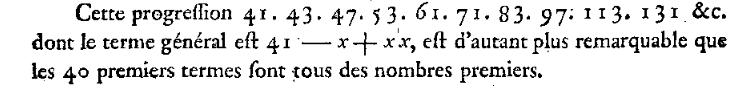
\includegraphics[width=12cm]{images/Euler_Prime.png}
\end{center}
Mit Mitteln der Zahlentheorie kann man zeigen, dass 
$p=41$ die größte Primzahl ist, für die das Polynom $X^2-X+p$ paarweise verschiedene Primzahlen für $X=1,\ldots,p-1$ liefert.
\item Das Polynom
\begin{align*}
f &= (k + 2) \bigg( 1  - [wz + h + j - q]^2  - [(gk + 2g + k + 1)(h + j) + h - z]^2 \\
& - [2n + p + q + z - e]^2  - [16(k + 1)^3(k + 2)(n + 1)^2 + 1 - f^2]^2 \\
&- [e^3(e + 2)(a + 1)^2 + 1 - o^2]^2 - [(a^2 - 1)y^2 + n - x^2]^2 \\
& - [16n^2y^4(a^2 - 1) + 1 - u^2]^2 \\
& - \bigg[ \bigg( (a + u^2(u^2 - a))^2 - 1 \bigg) (n + 4dy)^2 + 1 - (x + cu)^2 \bigg]^2 \\
& - [n + l + v - y]^2 - [(a^2 - 1)l^2 + 1 - m^2]^2  - [a + k + 1 - l - i]^2 \\
& - \bigg[ p + l(a - n - 1) + b (2an + 2a - n^2 - 2n - 2) - m \bigg]^2 \\
& - \bigg[ q + y(a - p - 1) + s (2ap + 2a - p^2 - 2p - 2) - x \bigg]^2 \\
& - \bigg[ z + pl(a - p) + t (2ap - p^2 - 1) - pm \bigg]^2 \bigg)
\end{align*}
aus dem Polynomring $\ZZ[a,b,\ldots,z]$ über $\ZZ$ in den 26 Variablen $a,b,\ldots,z$
hat die Eigenschaft, dass
\[
f(\NN^{26})\cap\NN=\PP
\]
ist, wobei $\PP$ die Menge aller Primzahlen ist\footnote{J. P. Jones, D. Sato, H. Wada and D. Wiens, Diophantine representation of the set of prime numbers, Amer. Math. Monthly, 83 (1976) 449-464}. Man beachte, dass das Polynom $f$ reduzibel ist. Schaut man sich den zweiten Faktor an, sieht man, dass die einzige Chance, einen positiven Wert zu erhalten,
darin besteht, dass alle Ausdrücke in eckigen Klammern Null werden. Man versuche mal, dass zu erreichen...
Der Nutzen dieses Polynoms ist eher überschaubar.
\end{enumerate}    
\end{bsp}

Im Folgenden wollen wir Polynome in einer Variablen besser verstehen.

\begin{defini}\label{def:grad_und_leitkoeffizient}
Sei $f = a_n X^n + a_{n-1} X^{n-1} + \cdots + a_1 X + a_0 \in R[X]$ mit $a_n \neq 0$. Dann heißt
\begin{itemize}
    \item $n$ der \defn{Grad} von $f$,
    \item $a_n$ der \defn{Leitkoeffizient} von $f$ .
\end{itemize}
Wir bezeichnen den Grad von $f$ mit $\deg(f)$ und den Leitkoeffizienten von $f$ mit $\ell(f)$.
Das Polynom $f$ heißt \defn{normiert}, falls $\ell(f) = 1$ gilt.
Zusätzlich setzen wir:
\[
\deg(0) := -\infty, \quad \ell(0) := 0.
\]
sowie
\[
R[X]_{< n} := \{ g \in R[X] \mid \deg(g) < n \}.
\]
\end{defini}

\begin{bem}\label{bem:eigenschaften_grad_und_leitkoeffizient}
Seien $f, g \in R[X]$. Dann gilt:
\begin{itemize}
    \item[(a)] $\ell(fg) = \ell(f) \ell(g)$, falls $\ell(f)$ oder $\ell(g)$ kein Nullteiler ist.
    \item[(b)] $\deg(fg) \leq \deg(f) + \deg(g)$, wobei Gleichheit gilt, falls $\ell(f)$ oder $\ell(g)$ kein Nullteiler ist.
    \item[(c)] $\deg(f+g) \leq \max(\deg(f), \deg(g))$, wobei Gleichheit gilt, falls $\deg(f) \neq \deg(g)$ ist.
\end{itemize}
\end{bem}

\begin{bem}\label{bem:eigenschaften_polynomring}
Es gilt:
\begin{itemize}
    \item[(a)] $R$ ist ein Integritätsring $\iff R[X_1, \dots, X_n]$ ist ein Integritätsring.
    \item[(b)] Ist $R$ ein Integritätsring, dann ist $R[X_1, \dots, X_n]^\times = R^\times$.
\end{itemize}
\end{bem}

\begin{proof}
Es genügt jeweils, (a) und (b) für $n = 1$ zu zeigen. Die Behauptung folgt dann in beiden Fällen per Induktion.

(a) Sei zunächst $R$ ein Integritätsring und seien $f, g \in R[X]$ mit $f, g \neq 0$. Es gilt $\deg(f), \deg(g) \geq 0$ und  deshalb nach \ref{bem:eigenschaften_grad_und_leitkoeffizient}:
    \[
    \deg(f g) = \deg(f) + \deg(g) \geq  0,
    \]
weswegen $fg\neq 0$ ist und damit $RX]$ ein Integritätsring. Die umgekehrte Implikation ergibt sich daraus, dass Unterringe von Integritätsringen wieder Integritätsringe sind.

(b) Sei $f \in R[X]^\times$. Dann existiert ein $g \in R[X]$ mit $f g = 1$. Aus 
\[0=\deg(f g)  = \deg(f) + \deg(g)\] folgt $\deg(f) = \deg(g) = 0$, also $f, g \in R$. Damit ist $f \in R^\times$. Umgekehrt ist jedes Element aus $R^\times$ auch ein Element von $R[X]^\times$.
\end{proof}

\begin{satz}\label{satz:polynomdivision}
Seien $f, g \in R[X]$ mit $\ell(f) \in R^\times$. Dann existieren eindeutig bestimmte Polynome $q, r \in R[X]$ mit
\[
g = q f + r \quad \text{und} \quad \deg(r) < \deg(f).
\]
\end{satz}

\begin{proof}
Der Beweis verläuft analog zu dem in der linearen Algebra für Körper geführten Beweis. Siehe auch das Skript zur Elementaren Zahlentheorie (EZT), Proposition 3.52.
\end{proof}

\begin{folgerung}\label{folgerung:polynomring-modul}
Sei $K$ ein Körper und $f \in K[X]\setminus\{0\}$ mit $\deg(f) = n$. Dann ist die $K$-Algebra $K[X]/(f)$ ein $K$-Vektorraum der Dimension $n$ mit Basis $(\overline{1}, \overline{X}, \dots, \overline{X}^{n-1})$\footnote{Über allgemeinem $R$ ist $R[X]/(f)$ für $f\in R[X]$
mit $\ell(f)\in R^\times$ ein freier $R$-Modul vom Rang $n$ mit Basis $(\overline{1}, \overline{X}, \dots, \overline{X}^{n-1})$. Der Beweis hierfür ist analog zum obigem.}.
\end{folgerung}

\begin{proof}
$K[X]/(f)$ wird zur $K$-Algebra über $K \hookrightarrow K[X] \to K[X]/(f)$ und dadurch auch zum $K$-Vektorraum. Aus Satz \ref{satz:polynomdivision} folgt die direkte Summen-Zerlegung von $K$-Vektorräumen
\[
K[X] = (f) \oplus K[X]_{<n},
\]
Die Projektion $K[X] \to K[X]/(f)$ induziert somit einen $K$-Vektorraumisomorphismus
\[
K[X]/(f) \cong K[X]_{<n}.
\]
Da $(1, X, \dots, X^{n-1})$ eine $K$-Basis von $K[X]_{<n}$ ist, folgt, dass $(\overline{1}, \overline{X}, \dots, \overline{X}^{n-1})$ eine $K$-Basis von $K[X]/(f)$ bildet.
\end{proof}

\begin{defini}\label{def:nullstelle}
Für $f \in R[X]$ heißt ein $a \in R$ eine \defn{Nullstelle} von $f$, falls $f(a) = 0$ gilt.
\end{defini}

\begin{bem}\label{bem:nullstellen-polynome}
Sei $f \in R[X]$. Dann sind äquivalent:
\begin{enumerate}[label=(\roman*)]
    \item $f(a) = 0$.
    \item Es existiert ein $q \in R[X]$ mit $f = (X - a)q$.
\end{enumerate}
Insbesondere gilt: Der Kern des Einsetzungshomomorphismus
\[
\Phi \colon R[X] \to R, \quad f \mapsto f(a)
\]
ist genau durch das Hauptideal $(X - a)$ gegeben. Da $\Phi$ surjektiv ist, induziert $\Phi$ einen Isomorphismus von $R$-Algebren
\[
R[X] / (X - a) \cong R.
\]
\end{bem}
\begin{proof}
"`(i) $\Rightarrow$ (ii)"': Nach Satz~\ref{satz:polynomdivision} existieren wegen $\ell(X - a) = 1 \in R^\times$ Polynome $q, r \in R[X]$ mit
\[
f = (X - a)q + r \quad \text{und} \quad \deg(r) < \deg(X - a) = 1.
\]
Also ist $r$ konstant. Durch Einsetzen von $a$ ergibt sich:
\[
f(a) = (a - a)q(a) + r(a) = r(a),
\]
d.h. $r = 0$.

"`(ii) $\Rightarrow$ (i)"': ist klar, wegen (ii) ist nämlich $f(a) = (a - a)q(a)=0$.
\end{proof}

\begin{defini}\label{def:nullstellenordnung}
Sei $a \in R$ und $f\in R[X]$. Dann definieren wir die \defn{Vielfachheit} der Nullstelle $a$ von $f$ (\defn{Nullstellenordnung}) als
\[
\ord_a(f) := \sup \{n \in \NN_0 \mid \text{Es existiert } g \in R[X] \text{ mit } f = (X - a)^n g \}.
\]
Ist $\operatorname{ord}_a(f) = 1$, so heißt $a$ eine \defn{einfache Nullstelle} von $f$.
Ist $\operatorname{ord}_a(f) > 1$, so heißt $a$ eine \defn{mehrfache Nullstelle} von $f$.
\end{defini}

\begin{anm}\label{anm:nullstellenordnung}
\begin{itemize}
    \item $f(a) = 0 \iff \operatorname{ord}_a(f) > 0$ (nach Bemerkung~\ref{bem:nullstellen-polynome}).
    \item Ist $f\neq0$, dann ist $\ord_a(f)\leq\deg(f)$, denn aus $f=(X-a)^ng$ folgt
    mit \ref{bem:eigenschaften_grad_und_leitkoeffizient}, dass $\deg(f)=n+\deg (g)$ ist.
    \item Ist $R$ ein Integritätsring, so ist $X-a$ ein Primelement in $R[X]$ wegen
    $R[X]/(X-a)\cong R$. Wir erhalten genau $\ord_a=v_{X-a}$ aus \ref{bsp:diskrete_bewertung}(b). Wegen der zuvor aufgelisteten Eigenschaft ist (a') aus \ref{bem:p-adische_bewertung} erfüllt. Es gilt also für alle $f,g\in R[X]$:
    \begin{align*}
        &\ord_a(f) = \infty \iff f=0 \\
        &\ord_a(fg) = \ord_a(f) + \ord_a(g), \\
        &\ord_a(f + g) \geq \min\{\ord_a(f), \ord_a(g)\}.
    \end{align*}
    Ohne die Voraussetzung, dass $R$ ein Integritätsring ist, ist dies im Allgemeinen falsch. Sei zum Beispiel \[R = \mathbb{Z}/8\mathbb{Z}, \quad f = X - \overline{1}, \quad g = X + \overline{1},\quad a = \overline{3}.\] Dann ist $\operatorname{ord}_a(f) = \operatorname{ord}_a(g) = 0$, aber $\operatorname{ord}_a(fg) = \operatorname{ord}_a(X^2 - \overline{1}) = 1$, da
    \[
    X^2 - \overline{1} = (X - \overline{3})(X + \overline{3}).
    \]
    Ist $R$ ein Integritätsring, setzt sich $\ord_a$ nach \ref{bem:p-adische_bewertung}
    nach zu einer diskreten Bewertung auf $\Quot(R[X])=\Quot(R)(X)$ fort. Wir erhalten dadurch Nullstellenordnung (und Polstellenordnung) für rationale Funktionen.
\end{itemize}
\end{anm}

\begin{bem}\label{bem:summe-nullstellenordnung}
Sei $R$ ein Integritätsring und $f\in R[X]\setminus\{0\}$. Dann besitzt $f$ höchstens $\deg(f)$ verschiedene Nullstellen in $R$, und es gilt:
\[
\sum_{a \in R} \ord_a(f) \leq \deg(f).
\]
\end{bem}
\begin{proof}
Übung
\end{proof}

\begin{defini}\label{def:zerfall_linear}
Sei $K$ ein Körper und $f \in K[X]\setminus\{0\}$ mit $\deg(f) = n$. Wir sagen, $f$ \defn{zerfällt in Linearfaktoren}, falls es $a_1, \dots, a_n \in R$ und $c \in R$ gibt mit
\[
f = c (X - a_1) \cdot\ldots\cdot (X - a_n).
\]
Der Körper $K$ heißt \defn{algebraisch abgeschlossen}, falls jedes Polynom aus $K[X] \setminus \{0\}$ in Linearfaktoren zerfällt. Dazu äquivalent ist die Bedingung, dass 
jedes nichtkonstante Polynom aus $K[X]$ eine Nullstelle in $K$ besitzt. 
\end{defini}

\begin{anm}\label{anm:linfakt_teiler}
Zerfällt ein Polynom $f\in K[X]\setminus\{0\}$ in Linearfaktoren, so gilt dies auch für jeden Teiler $g$ von $f$, 
\begin{denn}
Jeder Primteiler von $g$ ist auch ein Primteiler von $f$, und dafür kommen
nur Polynome der Form $X-a$ mit $a\in K$ in Betracht, da $f$ in Linearfaktoren zerfällt.
Da $K[X]$ faktoriell ist, zerfällt auch $g$ in Linearfaktoren.
\end{denn}
\end{anm}

\begin{satz}[Fundamentalsatz der Algebra]\label{satz:fundamentalsatz_algebra}
Der Körper $\CC$ ist algebraisch abgeschlossen.
\end{satz}

\begin{proof}
Der Beweis wird typischerweise in der Funktionentheorie-Vorlesung geführt. Siehe dort für Details.
\end{proof}

\begin{defini}\label{def:nullstelle_in_A}
Sei $A$ eine kommutative $R$-Algebra und $f \in R[X]$. Dann können wir den Polynomring $A[X]$ betrachten. Aus der universellen Eigenschaft von $R[X]$ erhalten wir den Einsetzungshomomorphismus
\[
\Phi \colon R[X] \to A[X] \quad \text{ mit }\Phi(X) = X,
\]
für den also \[\Phi\left(\sum_{i=0}^n r_i X^i\right) = \sum_{i=0}^n (r_i)_A X^i\] ist.
Für $f\in R[X]$ setzen wir $f_A:=\Phi(f)\in A[X]$.
Anstelle von "`$f_A$ hat die Eigenschaft ..."' sagen wir meist "`$f$ hat die Eigenschaft ...
über $A$"'. Anstelle von $f_A$ schreiben wir häufig wieder $f$.
\end{defini}

\begin{bsp}\label{bsp:polynom_zerfall}
Sei $f = X^2 + 1 \in \RR[X]$. $f$ besitzt keine Nullstelle in $\RR$ und zerfällt daher nicht in Linearfaktoren. Über $\CC$ zerfällt $f$ hingegen in Linearfaktoren:
    \[
    X^2 + 1 = (X - i)(X + i),
    \]
Die vorangegangene Definition erklärt, was hier formal gemeint ist: $\CC$ ist eine $\RR$-Algebra über die Inklusion $\RR\hookrightarrow\CC$. Wie oben beschrieben erhalten wir dadurch
einen Ringhomomorphismus
\[
\Phi\colon\RR[X]\to\CC[X], 
\]
der ein reelles Polynom $\sum_i r_iX^i\in\RR[X]$ auf das komplexe Polynom $\sum_i (r_i)_\CC X^i\in\CC[X]$ abbildet. Hierbei ist $(r_i)_\CC$ das Bild der reellen Zahl $r_i$ unter der Inklusion von $\RR$ nach $\CC$, also nichts weiter als die reelle Zahl $r_i$, aufgefasst als Element von $\CC$. Wenn wir sagen, dass $f$ über $\CC$ in Linearfaktoren zerfällt, so meinen wir damit formal, dass das Polynom $f_\CC=X^2+1\in\CC[X]$ in Linearfaktoren zerfällt.
\end{bsp}

\begin{defini}\label{def:formale_ableitung}
Sei $f = a_n X^n + \ldots + a_1 X + a_0 \in R[X]$. Dann definieren wir die \defn{formale Ableitung} von $f$ als
\[
f' := n a_n X^{n-1} + (n-1) a_{n-1} X^{n-2} + \ldots + a_1\in R[X].
\]
Wir setzen $f^{(0)}:=f$ und für $n\in\NN_0$ setzen wir induktiv $f^{(n+1)}:=(f^{(n)})'$.
\end{defini}

\begin{bsp}\label{bsp:ableitung_beispiele}
\begin{itemize}
    \item[(a)] Sei $f = X^3 - 7X^2 + 37 \in \QQ[X]$. Dann ist $f' = 3X^2 - 14X$.
    \item[(b)] Sei $f = X^4 + X^3 \in \FF_3[X]$. Dann ist $f' = \overline{4}X^3 + \overline{3}X^2 = X^3$.
    \item[(c)] Sei $f = X^6 + X^3 + 1 \in \FF_3[X]$. Dann ist $f' = 0$.
\end{itemize}
\end{bsp}


\begin{bem}\label{bem:formale_ableitung}
Es gilt:
\begin{itemize}
    \item[(a)] Die Abbildung $D \colon R[X] \to R[X], \; f \mapsto f'$, ist $R$-linear.
    \item[(b)] Für $f \in R[X]$ ist $f' \in R[X]$ das eindeutig bestimmte Polynom, für das in $R[X, \varepsilon]$ (mit $\varepsilon$ als zusätzlicher Polynomvariable) gilt:
    \[
    f(X + \varepsilon) \equiv f + \varepsilon f' \mod \varepsilon^2,
    \]
    bzw. äquivalent dazu:
    \[
    \frac{f(X + \varepsilon) - f(X)}{\varepsilon} \equiv f' \mod \varepsilon.
    \]    
    \item[(c)] (Produktregel) Für $f, g \in R[X]$ gilt:
    \[
    (f g)' = f' g + f g'.
    \]
    \item[(d)] (Taylorentwicklung) Sind $f\in R[X]$ und $a \in R$ und gilt $2,\ldots,n\in R^\times$, dann gilt
    \[
    f \equiv \sum_{k=0}^n \frac{f^{(k)}(a)}{k!} (X - a)^k \mod (X - a)^{n+1}.
    \]
    Insbesondere gilt:
    \[
    f\equiv f(a)+f'(a)(X-a) \mod (X-a)^2.
    \]
\end{itemize}
\end{bem}
\begin{proof}
Übung
\end{proof}

\begin{folgerung}\label{bem:nullstellen_und_ableitungen}
Sei $f \in R[X]$, $a \in R$, $n \in \NN$ mit $2,\ldots,n\in R^\times$.
Dann sind äquivalent:
\begin{enumerate}
\item [(i)] $\ord_a(f) > n$
\item [(ii)] $f(a) = f'(a) = \ldots = f^{(n)}(a) = 0$.
\end{enumerate}
Insbesondere gilt:
\[
a \text{ ist eine mehrfache Nullstelle von } f \iff a \text{ ist eine gemeinsame Nullstelle von } f \text{ und } f'.
\]
\end{folgerung}
\begin{proof}
Übung
\end{proof}

\section{Teilbarkeit in Polynomringen}

\begin{notation}
In diesem Abschnitt sei $R$ stets ein faktorieller Ring mit $\Quot(R) = K$. Es sei daran erinnert, dass wir für jedes Primelement $p\in R$ eine dazugehörige $p$-adische Bewertung $v_p$ auf $K$ haben, siehe \ref{bem:vp_diskrete_bewertung}. Wir fixieren ein Vertretersystem $\PP$ von Primelementen von $R$ modulo "`$\assoc$"'. Für den Ring $\ZZ$ nehmen wir dafür immer die Menge aller Primzahlen. 
\end{notation}

In diesem Abschnitt wollen wir zeigen, dass $R[X]$ faktoriell ist. Wir reduzieren dazu die Teilbarkeitstheorie von $R[X]$ auf die der beiden faktoriellen Ringe $R$ und $K[X]$.


\begin{bem}\label{bem:prim_element_in_R_auch_in_RX}
Sei $a\in R$. Dann induziert die koeffizientenweise Projektionsabbildung
\[
R[X] \to R / (a)[X], \quad f=\sum_{i=0}^n a_i X^i \mapsto f_{R/(a)}=\sum_{i=0}^n \overline{a_i} X^i
\]
einen Isomorphismus
\[
R[X]/(a) \cong R / (a)[X]
\]
Insbesondere gilt:
\[
a \text{ Primelement in } R \iff  a \text { Primelement in } R[X].
\]
\end{bem}

\begin{proof}
Die koeffizientenweise Projektionsabbildung ist surjektiv, und ihr Kern ist genau durch $(a)$
gegeben. Die erste Behauptung ergibt sich durch Anwendung des Homomorphiesatzes.
Wir erhalten
\begin{align*}
a\text{ Primelement in } R &\iff R / (a) \text{ Int.ring} \overset{\ref{bem:eigenschaften_polynomring}}{\iff} R / (a)[X] \text{ Int.ring} 
\iff R[X] / (a) \text{ Int.ring} \\
&\iff \text{$a$ Primelement in } R[X].
\end{align*}
\end{proof}

\begin{anm}
Die koeffizientenweise Projektionsabbildung ist ein Spezialfall der Konstruktion aus \ref{def:nullstelle_in_A}:
$A=R/(a)$ ist eine $R$-Algebra über die kanonische Projektion $R\to R/(a)$. Die Abbildung \[\Phi\colon R[X]\to A[X]=R/(a)[X], \quad f\mapsto f_A=f_{R/(a)}\]
aus \ref{def:nullstelle_in_A} ist genau durch
\[
\Phi(\sum_{i=0}^n r_i X^i) = \sum_{i=0}^n (r_i)_A X^i = \sum_{i=0}^n \overline{r_i} X^i
\]
gegeben.
\end{anm}

\begin{bem}\label{bem:diskrete_bewertung_polynome}
Sei $p \in R$ ein Primelement. Dann erfüllt die Abbildung
\begin{align*}
v_p\colon R[X]\to\NN_0\cup\{\infty\}, \quad f = a_n X^n + \ldots + a_0 \mapsto \sup \{ n \in \NN_0 \ \mid \ p^n \mid f \}
\end{align*}
die Eigenschaft (a') aus \ref{bem:p-adische_bewertung}, d.h. es gilt \[v_p(f) = \infty \iff f = 0.\]
Wir erhalten dadurch eine diskrete Bewertung auf $\Quot(R[X]) = K(X)$, die wir im Folgenden auf $K[X]\subseteq K(X)$ einschränken:
\[
v_p \colon K[X] \to \ZZ \cup \{\infty\}.
\]
Für $f = a_n X^n + \ldots + a_0 \in K[X]$ ist
\[
v_p(f) = \min \{ v_p(a_0), \ldots, v_p(a_n) \}.
\]
$v_p$ setzt die $p$-adische Bewertung auf $K$ fort, wir nennen sie die \defn{$p$-adische Bewertung} auf $K(X)$.
\end{bem}

\begin{proof}
Sei $f = a_n X^n + \ldots + a_0 \in R[X] \setminus \{0\}$. Dann gilt:
\[
p^n \mid f \iff p^n \mid a_0, \ldots, p^n \mid a_n.
\]
Daraus folgt $v_p(f) = \min \{ v_p(a_0), \ldots, v_p(a_n) \} < \infty$ und damit nach \ref{bem:p-adische_bewertung} die
Aussage über die Fortsetzbarkeit.
Ist $f=a_nX^n+\ldots+a_0\in K[X]$, so bringen wir die Koeffizienten von $f$ zunächst auf einen gemeinsamen Nenner, d.h. wir schreiben
\[
f=\frac{b_n}{d}X^n+\ldots+\frac{b_1}{d}X+\frac{b_0}{d}
\]
für $b_0,\ldots,b_n\in R$, $d\in R\setminus\{0\}$. Es ist dann
\[
f=\frac{b_n X^n + \ldots + b_0}{d}
\]
und deshalb
\begin{align*}
v_p(f)&=v_p(b_n X^n + \ldots + b_0)-v_p(d)= \min \{ v_p(b_0), \ldots, v_p(b_n) \} -v_p(d) \\
&= \min \{ v_p(b_0)-v_p(d), \ldots, v_p(b_n)-v_p(d) \} = \min \{ v_p(a_0), \ldots, v_p(a_n) \}
\end{align*}
\end{proof}

\begin{anm}
Besonders wichtig ist für uns im Folgenden die Eigenschaft
\[
v_p(fg)=v_p(f)+v_p(g)
\]
für alle $f,g\in K[X]$ (die zu den Eigenschaften einer diskreten Bewertung gehört und die in \ref{bem:p-adische_bewertung} in einem allgemeineren Kontext gezeigt wurde).   
\end{anm}

\begin{bsp}\label{bsp:bewertung_polynome}
$R = \ZZ$, $f = 15 T^2 + \frac{9}{4} T + \frac{27}{2} \in \QQ[T]$. Wir erhalten
\begin{align*}
v_2(f) &= \min \big\{ v_2(15), v_2\big(\frac{9}{ 4}\big), v_2\big(\frac{27}{2}\big) \big\} = \min \{0, -2, -1\} = -2,\\
v_3(f) &= \min \big\{ v_3(15), v_3\big(\frac{9}{4}\big), v_3\big(\frac{27}{2}\big) \big\} = \min \{1, 2, 3\} = 1,\\
v_p(f) &= 0 \quad \text{für alle Primzahlen } p \neq 2,3.
\end{align*}
\end{bsp}

\begin{bem}\label{bem:bewertung_von_polynomen}
Sei $f \in K[X] \setminus \{0\}$. Dann gilt:
\begin{enumerate}[label=(\alph*)]
    \item $v_p(f) = 0$ für fast alle $p \in \PP$.
    \item $f \in R[X] \iff v_p(f) \geq 0$ für alle $p \in \PP$.
\end{enumerate}
\end{bem}

\begin{proof}
(a) Es ist $v_p(f) \neq 0$ höchstens für die endlich vielen Primteiler von Zähler und Nenner der Koeffizienten in gekürzter Darstellung.

(b) Sei $f = a_n X^n + \ldots + a_0$. Dann gilt
\begin{align*}
f \in R[X] &\iff a_0, \ldots, a_n \in R \\
    &\iff v_p(a_0), \ldots, v_p(a_n) \geq 0 \quad \text{für alle } p \in \PP \\
    &\iff \min \{v_p(a_0), \ldots, v_p(a_n)\} \geq 0 \quad \text{für alle } p \in \PP \\
    &\iff v_p(f) \geq 0 \quad \text{für alle } p \in \PP.
\end{align*}
\end{proof}

\begin{defini}
Sei $f=a_nX^n+\ldots+a_0\in R[X]\setminus\{0\}$. Dann heißt das Polynom $f$ \defn{primitiv}, wenn $\ggT(a_0,a_1,\ldots,a_n)=1$ ist.    
\end{defini}

\begin{anm}\label{anm:primitive_polynome}
\begin{itemize}
\item Jedes normierte Polynom in $R[X]$ ist primitiv.
    \item Sei $f = a_n X^n + \ldots + a_0 \in R[X] \setminus \{0\}$. Dann ist
    \[
    \ggT(a_0, \ldots, a_n) \overset{\ref{bem:ggt_faktorieller_ring}}{=} \prod_{p \in \mathbb{P}} p^{\min\{v_p(a_0), \ldots, v_p(a_n)\}} = \prod_{p \in \mathbb{P}} p^{v_p(f)}
    \]
    Insbesondere ist $f$ ist genau dann primitiv, wenn $v_p(f) = 0$ für alle $p\in\PP$ ist.
\end{itemize}
\end{anm}

\begin{bem}\label{bem:primitiver_anteil}
Sei $f \in K[X] \setminus \{0\}$. Dann existieren ein Element $\cont(f)\in K^\times$ und 
ein primitives Polynom $\pp(f)\in R[X]$ mit
\[
f=\cont(f)\pp(f)
\]
Sowohl $\cont(f)$ als auch $\pp(f)$ sind eindeutig bis auf Multiplikation mit Elementen aus $R^\times$\footnote{In Fortsetzung der Schreibweise, die wir bereits für den $\ggT$ verwendet haben, schreiben wir im folgenden trotzdem immer "`$=$"', auch wenn häufig nur Gleichheit bis auf Multiplikation mit Elementen aus $R^\times$ besteht.}. Wir nennen $\cont(f)$ den \defn{Inhalt} von $f$ und $\pp(f)$ den \defn{primitiven Anteil} von $f$. Explizit ist
\[
\cont(f)=\prod_{p \in \mathbb{P}} p^{v_p(f)}\in K^\times.
\]
Es gilt:
\[
f\in R[X] \text{ und } f \text{ primitiv } \iff \cont(f)=1 \iff \pp(f)=f. 
\]
Für $f=a_nX^n+\ldots+a_0\in R[X]\setminus\{0\}$ ist
\[
\cont(f)=\ggT(a_0, \ldots, a_n)\in R.
\]
\end{bem}
\begin{proof}
Wir setzen
\[
\cont(f)=\prod_{p \in \mathbb{P}} p^{v_p(f)}\in K^\times, \quad \pp(f) := \frac{f}{\cont(f)} \in K[X].
\]
Für alle $p \in \mathbb{P}$ ist
\[
v_p(\pp(f)) = v_p\left(\frac{f}{\cont(f)}\right) \stackrel{\ref{bem:p-adische_bewertung}}{=} v_p(f) - v_p(\cont(f)) = v_p(f) - v_p(f) = 0.
\]
Wegen \ref{bem:bewertung_von_polynomen} liegt $\pp(f)$ in $R[X]$, und wegen \ref{anm:primitive_polynome} ist $\pp(f)$ primitiv.
Sei
\[
f = \cont(f) \cdot \pp(f) = c \cdot \tilde{f}
\]
mit $c \in K^\times$ und $\tilde{f} \in R[X]$ primitiv. Dann folgt
\[
v_p(\cont(f)) + v_p(\pp(f)) = v_p(c) + v_p(\tilde{f}).
\]
Daraus ergibt sich
\[
v_p(\cont(f)) - v_p(c) = 0 
\]
und deshalb $v_p\left(c^{-1}\cont(f)\right) = 0$.
Da dies für alle $p\in\PP$ gilt, erhalten wir aus \ref{bem:vp_diskrete_bewertung}, dass $c^{-1}\cont(f)$
in $R^\times$ liegt. Also ist $c \in \cont(f)R^\times$ und $\tilde{f} \in \pp(f)R^\times$. Die Charakterisierung
primitiver Polynome in $R[X]$ ergibt sich unmittelbar, und die Beschreibung des Inhalts von Polynomen aus $R[X]$ durch
den ggT der Koeffizienten folgt aus \ref{anm:primitive_polynome}.
\end{proof}

\begin{bsp}\label{bsp:inhalt_und_bewertung}
Sei $R = \ZZ$ und
\[
f = 15 T^2 + \frac{9}{4} T + \frac{27}{2} \in \QQ[T].
\]
Nach Beispiel \ref{bsp:bewertung_polynome} gilt:
\[
\cont(f) = 2^{-2} \cdot 3^1 = \frac{3}{4}.
\]
Es ist
\[
f = \frac{3}{4} \cdot \underbrace{(20T^2 + 3T + 18)}_{\pp(f)}
\]
und $\pp(f)$ ist ein primitives Polynom aus $\ZZ[X]$ wegen $\ggT(20, 3, 18) = 1$.
Da Primfaktorzerlegungen eher aufwendig zu berechnen sind, wäre es effizienter gewesen,
zur Bestimmung von $\cont(f)$ und $\pp(f)$ die Koeffizienten von $f$ zunächst auf einen gemeinsamen Nenner zu bringen und dann gemeinsame Faktoren herauszuziehen:
\[
f= 15 T^2 + \frac{9}{4} T + \frac{27}{2}=\frac{1}{4}(60T^2+9T+54)=\frac{3}{4}(20T^2+3T+18).
\]
\end{bsp}

\begin{satz}[Lemma von Gauß]\label{satz:gauss_lemma}
Seien $f, g \in K[X] \setminus \{0\}$. Dann gilt:
\begin{enumerate}[label=(\alph*)]
    \item $\cont(fg) = \cont(f) \cdot \cont(g)$.
    \item Sind $f, g$ in $R[X]$ und primitiv, dann ist $fg$ primitiv.
    \item $\pp(fg) = \pp(f) \cdot \pp(g)$.
\end{enumerate}
\end{satz}

\begin{proof}
(a) Es ist
    \begin{align*}
    \cont(fg) &= \prod_{p \in \mathbb{P}} p^{v_p(fg)} \stackrel{\text{\ref{bem:diskrete_bewertung_polynome}}}{=} \prod_{p \in \mathbb{P}} p^{v_p(f) + v_p(g)} = \left( \prod_{p \in \mathbb{P}} p^{v_p(f)} \right) \left( \prod_{p \in \mathbb{P}} p^{v_p(g)} \right) \\
    &= \cont(f) \cdot \cont(g).
    \end{align*}
(b) folgt aus (a).

(c) Für $f, g \in K[X] \setminus \{0\}$ ist
    \[
    \pp(fg) = \frac{fg}{\cont(fg)} \stackrel{\text{(a)}}{=} \frac{f}{\cont(f)} \cdot \frac{g}{\cont(g)} = \pp(f) \cdot \pp(g).
    \]
\end{proof}

\begin{folgerung}\label{folg:teilbarkeit_im_polring}
Seien $f, g \in R[X] \setminus \{0\}$. Dann sind äquivalent:
\begin{enumerate}[label=(\roman*)]
    \item $f\mid g$ in $R[X]$.
    \item $\cont(f) \mid \cont(g)$ in $R$ und $\pp(f) \mid \pp(g)$ in $R[X]$.
    \item $\cont(f) \mid \cont(g)$ in $R$ und $f\mid g$ in $K[X]$.
\end{enumerate}
Ist insbesondere $f$ primitiv, dann gilt:
\[
f\mid g \text{ in } R[X] \iff f\mid g \text{ in } K[X].
\]
\end{folgerung}

\begin{proof}
"`(i)$\Rightarrow$(ii)"': Aus $f\mid g \in R[X]$ folgt, dass es ein $h \in R[X]$ gibt mit $g = h \cdot f$. Nach Satz~\ref{satz:gauss_lemma} gilt
\[
\cont(g) = \cont(h) \cdot \cont(f),
\]
und
\[
\pp(g) = \pp(h) \cdot \pp(f),
\]
woraus sich (ii) ergibt.

"`(ii)$\Rightarrow$(i)"': Es gilt $g = \cont(g) \cdot \pp(g)$ und nach Voraussetzung $\cont(f) \mid \cont(g)$ sowie $\pp(f) \mid \pp(g)$. Daher folgt:
\[
f = \cont(f) \cdot \pp(f) \mid \cont(g) \cdot \pp(g) =g .
\]

Für den Nachweis der Äquivalenz von (ii) und (iii) bemerken wir zunächst, dass in $K[X]$ die Bedingung $f\mid g$ äquivalent zu $\pp(f)\mid\pp(g)$ ist, weil sich $f,\pp(f)$ bzw. $g,\pp(g)$ jeweils nur um eine Einheit in $K[X]$ unterscheiden.

"`(ii)$\Rightarrow$(iii)"' ist trivial.

"`(iii)$\Rightarrow$(ii)"': Wegen (iii) existiert ein $h \in K[X]$ mit $\pp(g) = h \cdot \pp(f)$. Damit erhalten wir
\[
1 = \cont(\pp(g)) = \cont(h \cdot \pp(f)) \stackrel{\text{\ref{satz:gauss_lemma}}}{=} \cont(h) \cdot \cont(\pp(f))
=\cont(h),\]
d.h. $h$ liegt nach \ref{bem:primitiver_anteil} in $R[X]$, womit (ii) gezeigt ist.
\end{proof}


\begin{bem}\label{bem:polynomringe_primelemente}
Sei $f \in R[X]$.
\begin{itemize}
    \item[(a)] Falls $f$ konstant ist, dann gilt:
    \[
    f \text{ Primelement in } R[X] \iff f \text{ Primelement in } R.
    \]
    \item[(b)] Falls $f$ nicht konstant ist, dann gilt:
    \[
    f \text{ Primelement in } R[X] \iff f \text{ primitiv und Primelement in } K[X].
    \]
\end{itemize}

\begin{proof}
(a) ist eine Wiederholung von \ref{bem:prim_element_in_R_auch_in_RX}.

(b) Sei $f$ nicht konstant.

"$\Rightarrow$"': Sei $f$ ein Primelement in $R[X]$. Wegen \ref{bem:primelement_irreduzibel} ist $f$ irreduzibel in $R[X]$ und damit $\cont(f)=1$, also $f$ primitiv. Seien $g,h\in K[X]$ mit $f\mid gh$ in K[X]. Dann gilt auch $f\mid\pp(gh)=\pp(g)\pp(h)$ in $K[X]$ und wegen
\ref{folg:teilbarkeit_im_polring} auch in $R[X]$. Da $f$ ein Primelement in $R[X]$ ist, folgt $f\mid\pp(g)$
oder $f\mid\pp(h)$ in $R[X]$ und damit $f\mid g$ oder $f\mid h$ in $K[X]$.

"$\Leftarrow$"': 
%Sei $f$ ein Primelement in $K[X]$ und primitiv. 
Seien $g,h\in R[X]$ mit $f\mid gh$.
Da $f$ Primelement in $K[X]$ ist, gilt in $K[X]$: $f\mid g$ oder $f\mid h$, ohne Einschränkung $f\mid g$. Da $f$ primitiv ist, folgt aus \ref{folg:teilbarkeit_im_polring}, dass $f\mid g$ auch in $R[X]$ gilt.
\end{proof}
\end{bem}

\begin{satz}\label{satz:polynomring_faktoriell}
$R[X]$ ist faktoriell. Ist $f \in R[X] \setminus \{0\}$, so setzt sich eine PFZ von $f$ zusammen aus einer PFZ von $\cont(f)$ in $R$ und einer PFZ von $\pp(f)$ in $K[X]$ mit primitiven Faktoren.
\end{satz}

\begin{proof}
Sei $f \in R[X] \setminus \{0\}$. Dann gilt:
\[
f = \cont(f) \pp(f).
\]
Da $\cont(f) \in R \setminus \{0\}$ ist und $R$ faktoriell ist, besitzt $\cont(f)$ eine PFZ in $R$. Diese ist wegen \ref{bem:polynomringe_primelemente} auch eine PFZ in $R[X]$.
Weil $K[X]$ euklidisch und daher faktoriell ist, besitzt $\pp(f)$ eine PFZ in $K[X]$, etwa
\[
\pp(f) = \prod_{i=1}^n p_i^{w_i}.
\]
Da $p_i, \pp(f_i)$ sich nur um Faktoren aus $R \setminus \{0\}$, also insbesondere nur um Einheiten aus $K^\times$, unterscheiden, ist
\[
\pp(f) = \prod_{i=1}^n \pp(p_i)^{w_i} \tag{*} \label{eq:PFZ_poly}
\]
auch eine PFZ von $\pp(f)$ in $K[X]$, wobei die $\pp(p_i)\in R[X]$ primitiv sind und Primelemente in $K[X]$. Damit sind die $\pp(p_i)$ nach \ref{bem:polynomringe_primelemente} Primelemente in $R[X]$ und \eqref{eq:PFZ_poly} ist eine PFZ von $\pp(f)$ in $R[X]$.
Insgesamt erhalten wir aus der PFZ von $\cont(f)$ und der PFZ von $\pp(f)$ eine PFZ von $f$
in $R[X]$.
\end{proof}

\begin{folgerung}\label{folgerung:polynomringe_mehrere_variablen}
$R[X_1, \dots, X_n]$ ist faktoriell.
\end{folgerung}

\begin{proof}
Dies folgt induktiv aus \ref{satz:polynomring_faktoriell}.
\end{proof}

\begin{anm}\label{anm:polynomringe_irreduzibel_vs_prim}
Da $R[X]$ faktoriell ist (genauso wie $R$ und $K[X]$), sind die Begriffe "`Primelement"' und "`irreduzibles Element"' in $R[X]$ nach \ref{folg:irreduzibel_prim_faktoriell} äquivalent. Man kann in \ref{bem:polynomringe_primelemente} auch jeweils „irreduzibel“ statt „Primelement“ schreiben. Für Polynome ist die Bezeichnung „irreduzibles Polynom“ gebräuchlich.
\end{anm}

\begin{bsp}\label{bsp:polynomring_kein_hjr}
$\ZZ[X]$ ist faktoriell (nach \ref{satz:polynomring_faktoriell}, da $\ZZ$ faktoriell), aber kein Hauptidealring. Das Ideal $(2, X)$ ist kein Hauptideal,
\begin{denn}
Die Elemente $2$ und $X$ sind beides Primelemente in $\ZZ[X]$ und sind nicht zueinander assoziiert. Damit ist $\ggT(2,X)=1$. Wäre $(2,X)$ ein Hauptideal, so wäre $(2,X)=(1)$ nach \ref{bem:ggT_hauptideal}, insbesondere würden $a,b\in\ZZ[X]$ mit $2a+Xb=1$ existieren. Setzen wir $X=0$, erhalten wir $2a(0)=1$, was zum Widerspruch führt.
\end{denn}
\end{bsp}

Wir erhalten aus dem Lemma von Gauß zwei weitere nützliche Aussagen, die wir so  
auch schon vor \ref{satz:polynomring_faktoriell} hätten beweisen können. 

\begin{bem}
Es sei $f\in R[X]$ normiert und es seien $g,h\in K[X]$ normiert mit $f=gh$.
Dann liegen $g,h$ beide in $R[X]$.
\end{bem}
\begin{proof}
Da $f\in R[X]$ normiert ist, ist $\cont(f)=1$. Außerdem ist
\[
1=\ell(g)=\ell(\cont(g)\pp(g))=\cont(g)\ell(pp(g)),
\]
analog für $h$. Insbesondere liegen $\cont(g)^{-1}$, $\cont(h)^{-1}$ beide in $R$. Wir erhalten
\[
1=(\cont(f))^{-1}=(\cont(gh))^{-1}\overset{\ref{satz:gauss_lemma}}{=}\cont(g)^{-1}\cont(h)^{-1},
\]
weswegen $\cont(g)^{-1},\cont(h)^{-1}$ und damit auch $\cont(g),\cont(h)$ beides Einheiten in $R$ sind (in unserer verkürzenden Notation: $\cont(g)=\cont(h)=1$). Wegen \ref{bem:primitiver_anteil} liegen $g,h$ beide in $R[X]$.
\end{proof}

Die Äquivalenz von (i) und (ii) in der nächsten Aussage könnten wir mittlerweile auch aus \ref{bem:polynomringe_primelemente} und \ref{anm:polynomringe_irreduzibel_vs_prim}
schließen, im nachfolgenden Beweis wird ein direktes Argument dafür gegeben.

\begin{bem}\label{bem:irreduzibilitaet_polynomringe}
Sei $f \in R[X]$ nichtkonstant. Dann sind äquivalent:
\begin{itemize}
    \item[(i)] $f$ ist irreduzibel in $K[X]$.
    \item[(ii)] $\pp(f)$ ist irreduzibel in $R[X]$.
    \item[(iii)] $f$ lässt sich nicht als Produkt zweier nichtkonstanter Polynome aus $R[X]$ schreiben.
\end{itemize}
\begin{proof}
"`(i)$\Rightarrow$(ii)"': Sei $\pp(f)=gh$ mit $g,h\in R[X]$. Mit $f$ ist auch $\pp(f)$ irreduzibel in $K[X]$, in $K[X]$ gilt also $\pp(f)\mid g$ oder $\pp(f)\mid h$.
Da $\pp(f)$ primitiv ist, gelten die Teilbarkeitsbeziehungen nach \ref{folg:teilbarkeit_im_polring} schon in $R[X]$,
und damit ist $\pp(f)$ irreduzibel in $R[X]$.

"`(ii)$\Rightarrow$(iii)"': Sei $f=gh$ mit $g,h\in R[X]$. Nach \ref{satz:gauss_lemma} ist
$\pp(f)=\pp(g)\pp(h)$, was wegen der Irreduzibilität von $\pp(f)$ direkt $\pp(f)\mid\pp(g)$ oder $\pp(f)\mid \pp(h)$ nach sich zieht. Damit ist eines der beiden Polynome $g,h$ nichtkonstant.

"`(iii)$\Rightarrow$(i)"': Sei $f=gh$ mit $g,h\in K[X]$. Nach \ref{satz:gauss_lemma} ist
$\pp(f)=\pp(g)\pp(h)$ und deshalb $f=\cont(f)\pp(g)\pp(h)$. Wegen (iii) ist eines der Polynome $\pp(g),\pp(h)$ konstant und damit eines der Polynome $g,h$ eine Einheit in $K[X]$,
weswegen $f$ irreduzibel in $K[X]$ ist. 
\end{proof}
\end{bem}

Im Folgenden wollen wir Irreduzibilitätskriterien für Polynome herleiten.
Wir schwächen für den Moment unsere Voraussetzungen an $R$ etwas ab und fordern nur noch, dass $R$ ein Integritätsring ist.

\begin{defini}\label{bem:eisenstein_polynom}
Seien $R$ ein Integritätsring, $\mathfrak{p} \subseteq R$ ein Primideal und $f = a_n X^n + \dots + a_0 \in R[X]$ ein Polynom vom Grad $n\geq 1$. Dann heißt $f$ ein \defn{$\mathfrak{p}$-Eisensteinpolynom}, falls gilt:
\[
a_n \notin \mathfrak{p}, \quad a_0, \dots, a_{n-1} \in \mathfrak{p}, \quad a_0 \notin \mathfrak{p}^2.
\]
\end{defini}

\begin{anm}\label{anm:p_eisenstein_polynom}
Ist $p \in R$ ein Primelement und $\mathfrak{p} = (p)$, dann sind die obigen Bedingungen äquivalent zu:
\[
p \nmid a_n, \quad p \mid a_0, \dots, a_{n-1}, \quad p^2 \nmid a_0.
\]
In diesem Fall spricht man auch von einem \defn{$p$-Eisensteinpolynom}.
\end{anm}


\begin{bsp}\label{bsp:eisenstein_2_3}
Sei $R = \ZZ$ und $f = 3X^4 + 4X^3 + 6X + 2$. Dann ist $f$ ein 2-Eisensteinpolynom, aber kein 3-Eisensteinpolynom.
\end{bsp}

\begin{bem}\label{bem:eisenstein_kriterium}
Seien $R$ ein Integritätsring, $\mathfrak{p} \subseteq R$ ein Primideal und $f = a_n X^n + \dots + a_0 \in R[X]$ ein Polynom vom Grad $n\geq1$. Wir setzen
\[
\overline{f} := f_{R/\mathfrak{p}}=\overline{a_n}X^n+\ldots+\overline{a_0} \in (R / \mathfrak{p})[X].
\]
Es gelte eine der folgenden Aussagen:
\begin{itemize}
    \item[(I)] $a_n \notin \mathfrak{p}$ und $\overline{f}$ lässt sich in $(R / \mathfrak{p})[X]$ nicht als Produkt zweier nichtkonstanter Polynome schreiben.
    \item[(II)] $f$ ist ein $\mathfrak{p}$-Eisensteinpolynom.
\end{itemize}
Dann lässt sich $f$ nicht als Produkt zweier nicht-konstanter Polynome aus $R[X]$ schreiben.
\end{bem}

\begin{proof}
Wir zeigen die Aussage per Kontraposition.
Seien $g, h \in R[X]$ nichtkonstant mit $f = gh$. Dann gilt:
\[
1 \leq \deg g, \deg h < n.
\]
Wir unterscheiden nun nach den beiden Fällen (I) und (II).

(I) Es ist $a_n = \ell(g) \ell(h)$, weil $R$ ein Integritätsring ist. Aufgrund von $a_n \notin \mathfrak{p}$ erhalten wir $\ell(g) \notin \mathfrak{p}$ und $\ell(h) \notin \mathfrak{p}$.
    % \[
    % \ell(g) \notin \mathfrak{p}, \quad \ell(h) \notin \mathfrak{p}.
    % \]
Es ergibt sich $\deg\overline{g}=\deg g$, $\deg\overline{h}=\deg h$, weswegen
$\overline{f}=\overline{g}\overline{h}$ eine Zerlegung von $\overline{f}$ in ein Produkt
zweier nichtkonstanter Polynome ist.

(II) Wir setzen $k := \Quot(R / \mathfrak{p})$ und nehmen im Folgenden an, dass $f$ ein $\mathfrak{p}$-Eisensteinpolynom ist. Wir erhalten in $(R / \mathfrak{p})[X]$ die Gleichung
\[
 \overline{g} \cdot \overline{h} = \overline{f} = \overline{a_n} X^n
\]
hat. Wir betrachten diese Gleichung in $k[X] \supseteq (R / \mathfrak{p})[X]$. Der Ring $k[X]$ ist ein Hauptidealring nach \ref{folg:polynomring_hir}. $X$ ist ein Primelement in $k[X]$ und der einzige Primteiler von $\overline{a_n}X^n$. Daher ist $X$ der einzige Primteiler von $\overline{g}$ und $\overline{h}$ in $k[X]$. Es existieren daher $B, C \in k$ sowie $r, s \in \NN_0$, sodass gilt:
\[
\overline{g} = B X^r, \quad \overline{h} = C X^s \quad \text{ und } r + s = n.
\]
Damit liegen die Koeffizienten $B$ und $C$ schon in $R / \mathfrak{p}$, das heißt, es gibt $b, c \in R$ mit $B = \overline{b}$ und $C = \overline{c}$. Wegen $\deg g,\deg h<n$ sind auch $\deg \overline{g},\deg \overline{h}<n$, d.h. $r, s \geq 1$. Somit ist $\overline{g}(0) = 0$ und $\overline{h}(0) = 0$. Daraus ergibt sich $g(0) \in \mathfrak{p}$ und $h(0) \in \mathfrak{p}$ und schließlich $a_0 = g(0) h(0) \in \mathfrak{p}^2$, was im Widerspruch dazu steht, dass $f$ ein $\mathfrak{p}$-Eisensteinpolynom ist. 
\end{proof}

\begin{satz}[Irreduzibilitätskriterien]\label{satz:irreduzibilitaetskriterien}
Sei $R$ ein faktorieller Ring, $K = \Quot(R)$ und $\mathfrak{p} \subseteq R$ ein Primideal. Sei $f = a_n X^n + \dots + a_0 \in R[X]$ ein Polynom vom Grad $n\geq 1$. Es gelte eine der beiden Aussagen:
\begin{itemize}
    \item[(I)] (\textit{Reduktionskriterium}) $a_n \notin \mathfrak{p}$ und $f$ ist irreduzibel in $(R / \mathfrak{p})[X]$.
    \item[(II)] (\textit{Eisensteinkriterium}) $f$ ist ein $\mathfrak{p}$-Eisensteinpolynom.
\end{itemize}
Dann ist $f$ irreduzibel in $K[X]$. Ist $f$ außerdem primitiv, so ist $f$ irreduzibel in $R[X]$.
\end{satz}

\begin{proof}
Falls (I) oder (II) gilt, lässt sich $f$ nach \ref{bem:eisenstein_kriterium} nicht als Produkt zweier nicht-konstanter Polynome in $R[X]$ schreiben. Aus \ref{bem:irreduzibilitaet_polynomringe} folgt, dass $f$ irreduzibel in $K[X]$ ist und dass $f$ irreduzibel in $R[X]$ ist, falls $f$ prim ist.
\end{proof}

\begin{anm}\label{anm:reduktionskriterium_hir}
\begin{itemize}
\item Das Reduktionskriterium wird häufig angewandt, wenn $R$ ein Hauptidealring und $p\in R$ ein Primelement ist. Dann ist $(p)$ ein maximales Ideal in $R$ nach \ref{folg:irreduzibel_primelement_maximal}, also ist $R / (p)$ ein Körper und damit $(R /(p))[X]$ faktoriell.
\item Eine weitere Anwendung des Reduktionskriteriums ist wie folgt gegeben. Sei $R = k[X_1, \dots, X_n]$, wobei $k$ ein Körper ist und sei $p = X_n$ (dies ist ein Primelement). Dann gilt: $R / (p) = k[X_1, \dots, X_{n-1}]$, das Problem ist um eine Variable reduziert.

\end{itemize}
\end{anm}

\begin{bsp}\label{bsp:irreduzibilitaet_polynome}
\begin{itemize}
    \item[(a)] Sei $R = \ZZ$, $f = X^3 + 7X^2 + 4X - 15 \in \ZZ[X]$. Dieses Polynom ist irreduzibel in $\ZZ[X]$ und in $\QQ[X]$,
    \begin{denn}
    Wir wenden das Reduktionskriterium mit $\mathfrak{p} = (2)$ an. Es ist \[\overline{f} = X^3 + X^2 + \overline{1} \in \mathbb{F}_2[X]\] irreduzibel. Andernfalls hätte $\overline{f}$ wegen $\deg(\overline{f}) = 3$ einen Teiler vom Grad 1, also eine Nullstelle in $\mathbb{F}_2$. Es ist jedoch $\overline{f}(0) = \overline{1}$ und $\overline{f}(1) = \overline{1}$. Da $f$ primitiv ist, folgt aus dem Reduktionskriterium die Behauptung. 
    \end{denn}
    \item[(b)] Sei $f = X^3 + 5X + 5 \in \ZZ[X]$. Dieses Polynom ist irreduzibel in $\ZZ[X]$ und $\QQ[X]$, da $f$ ein $5$-Eisensteinpolynom ist.

    \item[(c)] Sei $p$ eine Primzahl. Dann ist das Polynom
    \[
    \Phi_p = X^{p-1} + X^{p-2} + \dots + 1 = \frac{X^p - 1}{X - 1} \in \ZZ[X]
    \]
    (das im späteren Verlauf der Vorlesung eine Rolle spielen wird) irreduzibel in $\ZZ[X]$ und $\QQ[X]$.
    \begin{denn} Das Polynom $\Phi_p$ ist genau dann irreduzibel, wenn $\Phi_p(X+1)$ irreduzibel ist.
Es ist
\begin{align*}
\Phi_p(X+1) &= \frac{(X+1)^p - 1}{X} = \frac{X^p + \binom{p}{1} X^{p-1} + \dots + \binom{p}{p-2} X^2 + \binom{p}{p-1} X}{X}\\
&= X^{p-1} + \binom{p}{1} X^{p-2} + \dots + \binom{p}{p-2} X + \binom{p}{p-1}.
\end{align*}
Hierbei teilt $p$ jeden der Binomialkoeffizienten $\binom{p}{i}$ für $i = 1, \dots, p-1$, denn \[\binom{p}{i} = \frac{p \cdot (p-1) \cdot \dots \cdot (p-i+1)}{1 \cdot 2 \cdot \dots \cdot i} \in \NN\] und $p$ teilt jeweils den Zähler, aber nicht den Nenner.
Außerdem teilt $p$ nicht den Binomialkoeffizienten $\binom{p}{p-1}=p$.
Somit ist $\Phi_p(X+1)$ ein primitives $p$-Eisensteinpolynom und daher irreduzibel in $\ZZ[X]$ und $\QQ[X]$.
    \end{denn}
    \item[(d)] Sei $R$ ein faktorieller Ring und $p\in R$ ein Primelement.
    Dann ist das Polynom \[f=X^n-p\in R[X]\] aufgrund des Eisensteinkriteriums irreduzibel in $R[X]$ und in $\Quot(R)[X]$. Insbesondere ist für eine Primzahl $p$ das Polynom $X^n-p\in\ZZ[X]$ irreduzibel in $\QQ[X]$. Dies verschärft die Aussage aus \ref{bsp:diskrete_bewertung_auf_Q}(b), in der gezeigt wurde, dass es keine rationale Nullstelle besitzt. Ein weiterer Spezialfall ergibt sich, wenn $k$  
    ein Körper, $R = k[t]$ und \[f = X^n - t \in R[X]\]
    ist. Es ist $t$ ein Primelement in $R$, also ist $f$ irreduzibel in $R[X]$ und in $\Quot(R)[X] = k(t)[X]$.
\end{itemize}
\end{bsp}

\chapter{Algebraische Körpererweiterungen}
\setcounter{section}{7}
\section{Endliche und algebraische Körpererweiterungen}

\begin{defini}\label{def:erweiterungskörper}
Seien $L$ ein Körper und $K \subseteq L$ ein Teilkörper. Dann nennen wir $L$ einen \defn{Erweiterungskörper} von $K$ und $L|K$ eine \defn{Körpererweiterung}. Über die Inklusion $K\hookrightarrow L$ wird $L$ zu einer kommutativen $K$-Algebra. Die Dimension
\[[L : K] := \dim_K L \in \NN \cup \{\infty\}\] 
heißt der \defn{Grad} der Körpererweiterung $L|K$.
$L|K$ heißt \defn{endlich}, falls $[L : K] < \infty$ gilt.
\end{defini}

\begin{notation}
Für den Rest des Abschnitts sei $L|K$ eine Körpererweiterung.
\end{notation}

\begin{bsp}\label{bsp:koerpererweiterungen}
\begin{itemize}
    \item[(a)] $\CC|\RR$ ist eine Körpererweiterung mit $[\CC : \RR] = 2$.
    \item[(b)] $\RR|\QQ$ ist eine Körpererweiterung mit $[\RR : \QQ] = \infty$, denn wäre $[\RR : \QQ]=n \in \NN$, dann wäre $\RR\cong\QQ^n$ abzählbar, was ein Widerspruch ist.
    \item[(c)] Sei $K$ ein Körper, $R = K[X]$ und $K(X) = \Quot(K[X])$ (der Körper der rationalen Funktionen über $K$ in der Variablen $X$). Dann ist $K(X)|K$ eine Körpererweiterung mit $[K(X) : K] = \infty$, denn $(X^i)_{i \in \NN_0}$ ist eine unendliche $K$-linear unabhängige Familie von Elementen aus $K(X)$
\end{itemize}
\end{bsp}

\begin{bem}\label{bem:triviale_erweiterung}
Die folgenden Aussagen sind äquivalent:
\begin{itemize}
    \item[(i)] $[L : K] = 1$.
    \item[(ii)] $L = K$.
\end{itemize}
\begin{proof}
"`(i)"' $\Rightarrow$ (ii): Sei $x \in L$. Dann ist $(1, x)$ wegen $[L:K]=1$ linear abhängig über $K$. Somit existieren $a,b\in K$ mit $(a,b)\neq(0,0)$ und $a+bx=0$. Wäre $b=0$, dann würde $a=0$ folgen, was ein Widerspruch wäre. Also ist $b\neq0$ und deshalb
$x=-b^{-1}a\in K$.

"`(ii)"' $\Rightarrow$ (i): Dies ist trivial.
\end{proof}
\end{bem}

\begin{satz}[Gradsatz]\label{satz:gradsatz}
Sei $M|L|K$ eine Körpererweiterung ($L$ heißt dann auch ein \defn{Zwischenkörper} von $M|K$). Dann gilt:
\[
[M : K] = [M : L] \cdot [L : K].
\]
\end{satz}
\begin{proof}
Seien zunächst $M|L$ und $L|K$ endlich. Dann gilt:
    \[
    M \cong L^{[M:L]} \quad \text{als } L\text{-VR (also auch als $K$-VR)}, \quad L \cong K^{[L:K]} \quad \text{als } K\text{-VR}.
    \]
    Daher ergibt sich:
    \[
    M \cong \left(K^{[L:K]}\right)^{[M:L]} \cong K^{[L:K] \cdot [M:L]} \quad \text{als } K\text{-VR}.
    \]
    und daraus die Gradformel. Ist $[L : K] = \infty$, dann existieren unendlich viele $K$-linear unabhängige Elemente in $L$. Daher existieren auch in $M$ unendlich viele $K$-linear unabhängige Elemente. Somit ist $[M : K] = \infty$.
    Ist $[M : L] = \infty$, dann existieren unendlich viele $L$-linear unabhängige Elemente in $M$. Diese Elemente sind auch $K$-linear unabhängig. Somit ist $[M : K] = \infty$.
\end{proof}

\begin{anm}
Ist $(x_i)_{i\in I}$ eine Basis von $M$ als $L$-Vektorraum und $(y_j)_{j\in J}$ eine Basis von $L$ als $K$-Vektorraum,
dann ist $(x_iy_j)_{(i,j)\in I\times J}$ eine Basis von $M$ als $K$-Vektorraum.
\end{anm}

\begin{folgerung}\label{folgerung:primzahl_zwischenkörper}
Sei $M|L|K$ eine Körpererweiterung, wobei $[M : K]$ eine Primzahl ist. Dann gilt: $L = K$ oder $L = M$.
\end{folgerung}

\begin{proof}
Es gilt $[M : K] \overset{\ref{satz:gradsatz}}{=} [M : L] \cdot [L : K]$. Da $[M : K]$ eine Primzahl ist, folgt, dass entweder $[M : L] = 1$ oder $[L : K] = 1$. Im ersten Fall ist $M = L$, und im zweiten Fall ist $L = K$, jeweils wegen \ref{bem:triviale_erweiterung}.
\end{proof}

\begin{defini}\label{def:algebraisch_unabhängig}
Sei $\alpha\in L$. Das Element $\alpha$ heißt \defn{algebraisch über $K$}, falls $(\alpha)$ algebraisch abhängig über $K$ ist. Dies ist äquivalent dazu, dass eine der folgenden Bedingungen gilt (vgl. \ref {satz:ue_polynomrings}):
\begin{itemize}
    \item Es existiert ein $f \in K[X]$, $f \neq 0$ mit $f(\alpha) = 0$ .
    \item Der $K$-Algebrenhomomorphismus $\Phi_\alpha : K[X] \to L, \quad f \mapsto f(\alpha)$ ist nicht injektiv.
\end{itemize}
Andernfalls heißt $\alpha$ \defn{transzendent} über $K$.
\end{defini}

\begin{bsp}\label{bsp:algebraisch_transzendent}
\begin{itemize}
    \item[(a)] $\sqrt{2} \in \RR$ ist algebraisch über $\QQ$, denn für $f(X) = X^2 - 2 \in \QQ[X]$ ist $f(\sqrt{2})=0$.
    \item[(b)] $\pi$ ist transzendent über $\QQ$ (Satz von Lindemann, 1882).
    \item[(c)] $\pi$ ist algebraisch über $\RR$, denn für $f(X) = X - \pi \in \RR[X]$ ist $f(\pi)=0$.
\end{itemize}
\end{bsp}

\begin{defini}\label{def:algebraische_koerpererweiterung}
$L|K$ heißt \defn{algebraisch}, falls jedes Element aus $L$ algebraisch über $K$ ist.
\end{defini}

\begin{bsp}\label{bsp:algebraische_erweiterung}
\begin{itemize}
    \item[(a)] $\CC|\RR$ ist algebraisch, denn $\alpha = a + bi \in \CC$ mit $a, b \in \RR$ ist Nullstelle von $X^2-2aX+(a^2+b^2)\in\RR[X]$.
    \item[(b)] Es bezeichne $K(X)$ den Körper der rationalen Funktionen über $K$ in der Variablen $X$. Die Körpererweiterung $K(X)|K$ ist nicht algebraisch, da die Variable $X$ algebraisch unabhängig über $K$, also transzendent über $K$ ist.
\end{itemize}
\end{bsp}

\begin{defini}\label{def:erzeugte_unterkoerper}
Seien $\alpha_1, \dots, \alpha_n \in L$. Dann heißt
\[
K(\alpha_1, \dots, \alpha_n) := \Quot(K[\alpha_1, \dots, \alpha_n]) \subseteq L
\]
der \defn{von $\alpha_1, \dots, \alpha_n$ über $K$ erzeugte Teilkörper} von $L$ ("`\defn{$K$ adjungiert $\alpha_1,\ldots,\alpha_n)$}"'). Die Körpererweiterung $L|K$ heißt \defn{endlich erzeugt}, falls es $\beta_1, \dots, \beta_n \in L$ mit $L = K(\beta_1, \dots, \beta_n)$ gibt. Sie heißt \defn{einfach}, falls ein $\beta\in L$ mit $L = K(\beta)$ existiert.
\end{defini}

\begin{anm}
\begin{itemize}
\item Es ist
\begin{align*}
K[\alpha_1,\ldots,\alpha_n]&=\{f(\alpha_1,\ldots,\alpha_n)\mid f\in K[X_1,\ldots,X_n]\}\\
K(\alpha_1,\ldots,\alpha_n)&=\left\{\frac{f(\alpha_1,\ldots,\alpha_n)}{g(\alpha_1,\ldots,\alpha_n)} \mid f,g\in K[X_1,\ldots,X_n], g(\alpha_1,\ldots,\alpha_n)\neq 0\right\},
\end{align*}
insbesondere gilt für $\alpha\in L$:
    \[K[\alpha] = \{f(\alpha) \mid f \in K[X]\}, \quad K(\alpha) = \left\{\frac{f(\alpha)}{g(\alpha)} \mid f, g \in K[X], g(\alpha) \neq 0 \right\}.\]
    \item $K[\alpha_1, \dots, \alpha_n]$ ist der kleinste Unterring von $L$, der $K$ und $\alpha_1, \dots, \alpha_n$ enthält.
    \item $K(\alpha_1, \dots, \alpha_n)$ ist der kleinste Teilkörper von $L$, der $K$ und $\alpha_1, \dots, \alpha_n$ enthält.
\end{itemize}
\end{anm}

\begin{satz}\label{satz:minimalpolynom}
Sei $\alpha \in L$ algebraisch über $K$ und $\Phi_\alpha : K[X] \to L$, $f \mapsto f(\alpha)$. Dann gilt:
\begin{itemize}
    \item[(a)] Es gibt genau ein normiertes Polynom kleinsten Grades $\mipo_K\alpha \in K[X]$ mit $(\mipo_K\alpha)(\alpha) = 0$. Das Polynom $\mipo_K\alpha$ heißt das \defn{Minimalpolynom} von $\alpha$ über $K$
    \item[(b)] $\mipo_K\alpha$ ist irreduzibel.
     \item[(c)] $\ker \Phi_\alpha = (\mipo_K\alpha)$. Insbesondere gilt für $f\in K[X]$: 
     \[
     f(\alpha)=0\iff \mipo_k\alpha\mid f.
     \]
    \item[(d)] $\image \Phi_\alpha = K[\alpha]$.
    \item[(e)] $K[\alpha]$ ist ein Körper, d.h. $K[\alpha] = K(\alpha)$.
    \item[(f)] Es existiert ein eindeutig bestimmter $K$-Algebrenisomorphismus
    \[
    \overline{\Phi_\alpha}\colon K[X] / (\mipo_K\alpha) \to K(\alpha) \quad \text{mit } \overline{\Phi_\alpha}(\overline{X})=\alpha.
    \]
    \item[(g)] Die Familie $(1, \alpha, \alpha^2, \dots, \alpha^{\deg(\mipo_K\alpha)-1})$ ist eine $K$-Basis von $K(\alpha)$, insbesondere ist $K(\alpha)|K$ eine endliche Körpererweiterung. Ihr Grad $[K(\alpha) : K]=:\deg_K\alpha$ heißt der \defn{Grad von $\alpha$ über $K$}.
    \item[(h)] $\deg_K\alpha = \deg \mipo_K\alpha$.
\end{itemize}
\end{satz}

\begin{proof}
(a), (c) Da $\alpha$ algebraisch über $K$ ist, ist $\ker \Phi_\alpha \neq (0)$. Weil $K[X]$ ein Hauptidealring ist, existiert ein eindeutig bestimmtes normiertes Polynom $\mipo_K\alpha \in K[X]$ mit $\ker \Phi_\alpha = (\mipo_K\alpha)$. Unter allen normierten Polynomen in $\ker \Phi_\alpha$ ist $\mipo_K\alpha$ das eindeutig bestimmte Polynom kleinsten Grades.

(d) Dies folgt direkt aus der Definition.

(b), (e), (f): Nach der universellen Eigenschaft des Polynomrings ist $\Phi_\alpha: K[X] \to L$ der eindeutig bestimmte $K$-Algebrenhomomorphismus mit $\Phi_\alpha(X) = \alpha$. Daraus erhalten wir aus dem Homomorphiesatz einen eindeutig bestimmten $K$-Algebrenisomorphismus
\[
\overline{\Phi_\alpha}\colon K[X] / (f) \to K[\alpha] \quad \text{mit } \overline{\Phi_\alpha}(\overline{X}) = \alpha
\]

Da $K[\alpha]\subseteq L$ nullteilerfrei ist, ist $K[X] / (\mipo_K\alpha)$ nullteilerfrei. Somit ist $\mipo_K\alpha$ prim und daher irreduzibel. Weil $K[X]$ ein Hauptidealring ist, ist $(\mipo_K\alpha)$ wegen \ref{folg:irreduzibel_primelement_maximal} ein maximales Ideal, also $K[X] / (\mipo_K\alpha)$ ein Körper. Daher ist $K[\alpha]$ ein Körper und insbesondere gilt $K[\alpha] = K(\alpha)$.

(g), (h): Nach \ref{folgerung:polynomring-modul} ist $(\overline{1}, \overline{X}, \overline{X}^2, \dots, \overline{X}^{\deg(\mipo_K\alpha)-1})$ eine $K$-Basis von $K[X] / (\mipo_K\alpha)$. Somit ist \[(\Phi_\alpha(\overline{1}),\Phi_\alpha(\overline{X}),\ldots,\Phi_\alpha(\overline{X}^{\deg(\mipo_K\alpha)-1})) =(1,\alpha, \alpha^2, \dots, \alpha^{\deg(\mipo_K\alpha)-1})\] eine $K$-Basis von $K(\alpha)$. Daher folgt 
\[[K(\alpha) : K] = \dim_K K(\alpha) = \deg(\mipo_K\alpha).\]
\end{proof}

\begin{bem}\label{bem:minpol_char}
Sei $\alpha\in L$ algebraisch über $K$ und $f\in K[X]$ ein normiertes Polynom.
Dann sind äquivalent:
\begin{enumerate}[label=(\roman*)]
\item $f=\mipo_K(\alpha)$.
\item $f(\alpha)=0$ und $f$ ist irreduzibel.
\item $f(\alpha)=0$ und $\deg f=\deg_K\alpha$.
\end{enumerate}
\end{bem}
\begin{proof}
"`(i)$\Rightarrow$(ii)"' folgt aus \ref{satz:minimalpolynom}.

"`(ii)$\Rightarrow$(iii)"' Aus $f(\alpha)=0$ folgt mit \ref{satz:minimalpolynom}(c),
dass $\mipo_K\alpha\mid f$ gilt. Aus der Irreduzibilität von $f$ folgt $\deg(f)=\deg_K\alpha$.

"`(iii)$\Rightarrow$(i)"' Aus $f(\alpha)=0$ ergibt sich mit \ref{satz:minimalpolynom}(c),
dass $\mipo_K\alpha\mid f$ gilt. Da $f$ als normiertes Polynom vom Nullpolynom verschieden ist, erhalten wir
\[\deg_K\alpha=\deg\mipo_K\alpha\leq\deg f=\deg_K\alpha,\]
also $\deg f=\deg \mipo_K\alpha$. Da $f$ und $\mipo_K\alpha$ beide normiert sind, 
folgt $f=\mipo_K(\alpha)$.
\end{proof}

\begin{anm}
Das Minimalpolynom $\mipo_K \alpha$ stimmt mit dem Minimalpolynom (aus der linearen Algebra) des $K$-Vektorraum-Endomorphismus
\[
h: L \to L, \quad x \mapsto \alpha x
\]
überein.
\begin{denn}
Wegen $\mu_\alpha(1) = \alpha$ gilt 
\[
\mu_\alpha=0\iff \alpha=0
\]
und für $g \in K[X]$ ist $g(\mu_\alpha) = \mu_{g(\alpha)}$, und somit erhalten wir
\[
g(\mu_\alpha)=0\iff \mu_{g(\alpha)}=0 \iff g(\alpha)=0.
\]
\end{denn}
\end{anm}

\begin{bsp}\label{bsp:minimalpolynom_beispiel}
Es ist $\sqrt{3}\in\RR$ algebraisch über $\QQ$, denn es ist $f(\sqrt{3}) = 0$ für $f = X^2 - 3 \in \QQ[X]$.
Das Polynom $f$ ist irreduzibel nach dem Eisensteinkriterium, somit ist $f = \mipo_\QQ(\sqrt{3})$ wegen \ref{bem:minpol_char}.
Per Definition ist
\begin{align*}
\QQ[\sqrt{3}]&=\{g(\sqrt{3}) \ \ | \ g \in \QQ[X]\}, \\
\quad \QQ(\sqrt{3}) &= \left\{\frac{g(\sqrt{3})}{h(\sqrt{3})} \;\middle|\; g, h \in \QQ[X], h(\sqrt{3}) \neq 0 \right\}.
\end{align*}
Nach Satz \ref{satz:minimalpolynom} ist $\QQ[\sqrt{3}]=\QQ(\sqrt{3})$, $\QQ[\sqrt{3}]$ ist ein Körper und $(1, \sqrt{3})$ ist eine $\QQ$-Basis von $\QQ(\sqrt{3})$. Somit ist
\[
\QQ(\sqrt{3}) = \{a + b\sqrt{3} \mid a, b \in \QQ\}.
\]
Beispielsweise ist
\[\frac{1}{\sqrt{3}} = \frac{1}{3} \cdot \sqrt{3}.\]
Wegen Satz \ref{satz:minimalpolynom} ist $\QQ[X] / (X^2 - 3) \cong \QQ(\sqrt{3})$ als $\QQ$-Algebra.
\end{bsp}

\begin{bsp}\label{bsp:invers_koerpererweiterung}
Sei $\alpha \in L\setminus\{0\}$ algebraisch über $K$. Wie findet man $\alpha^{-1} \in K(\alpha)=K[\alpha]$?
Sei \[f = X^n + c_{n-1} X^{n-1} + \dots + c_0 \in K[X]\] das Minimalpolynom von $\alpha$ über $K$.
Für $n = 1$ ist $f = X + c_0$. Aus $f(\alpha) = 0$ folgt dann $\alpha + c_0 = 0$, also $\alpha = -c_0$ und deshalb \[\alpha^{-1} = -c_0^{-1} \in K \subseteq K[\alpha].\]
Im Fall $n \geq 2$ ist $c_0 \neq 0$, da $f$ irreduzibel ist (ist $c_0=0$ wäre $f$ durch $X$ teilbar). Dann ist
\[
0 = \alpha^{-1} f(\alpha) = \alpha^{-1} \big(\alpha^n + c_{n-1} \alpha^{n-1} + \dots + c_0 \big).
\]
Das ergibt
\[
-c_0 \alpha^{-1} = \alpha^{n-1} + c_{n-1} \alpha^{n-2} + \dots + c_1
\]
und schließlich
\[
\alpha^{-1} = -c_0^{-1} \big(\alpha^{n-1} + c_{n-1} \alpha^{n-2} + \dots + c_1\big) \in K[\alpha].
\]
\end{bsp}

\begin{satz}\label{satz:endl_erweiterung_aquivalenzen}
Es sind äquivalent:
\begin{itemize}
    \item[(i)] $L|K$ ist endlich.
    \item[(ii)] $L$ wird über $K$ von endlich vielen algebraischen Elementen erzeugt, d.h. es existieren Elemente $\alpha_1, \dots, \alpha_n \in L$, die algebraisch über $K$ sind, sodass $L = K(\alpha_1, \dots, \alpha_n)$ ist.
    \item[(iii)] $L|K$ ist eine endlich erzeugte algebraische Körpererweiterung, d.h. $L|K$ ist algebraisch und es existieren $\alpha_1, \dots, \alpha_n \in L$ mit $L = K(\alpha_1, \dots, \alpha_n)$.
\end{itemize}
Insbesondere ist jede endliche Körpererweiterung algebraisch. In diesem Fall ist $L = K[\alpha_1, \dots, \alpha_n]$ mit $\alpha_1, \dots, \alpha_n$ wie in (ii) oder (iii).
\end{satz}

\begin{proof}
"`(i) $\Rightarrow$ (iii)"': Sei $L|K$ endlich mit $n = [L : K]$ und sei $\alpha \in L$. Die $n+1$ Elemente $1, \alpha, \alpha^2, \dots, \alpha^n$ sind dann linear abhängig über $K$.
    Es existieren also $c_0, \dots, c_n \in K$, nicht alle gleich $0$, sodass
    \[
    c_n \alpha^n + \dots + c_1 \alpha + c_0 = 0
    \]
    ist. Daher ist $\alpha$ algebraisch über $K$. Somit ist $L|K$ algebraisch.
    Da $L|K$ endlich ist, existiert eine endliche $K$-Basis $(\alpha_1, \dots, \alpha_n)$ von $L$. Dann gilt:
    \[
    L = K\alpha_1 + \ldots + K\alpha_n \subseteq K(\alpha_1, \ldots, \alpha_n) \subseteq L,
    \]
    also $L = K(\alpha_1, \ldots, \alpha_n)$.

"`(iii) $\Rightarrow$ (ii)"': Sei $L|K$ algebraisch, und seien $\alpha_1, \dots, \alpha_n \in L$ mit $L = K(\alpha_1, \dots, \alpha_n)$. Daraus folgt, dass $\alpha_1, \dots, \alpha_n$ algebraisch über $K$ sind. 

"`(ii) $\Rightarrow$ (i)"':
Wir beweisen durch vollständige Induktion nach $n$ die folgende Aussage: Sind $\alpha_1, \dots, \alpha_n\in L$ algebraisch über $K$, dann ist $K(\alpha_1,\ldots,\alpha_n)=K[\alpha_1,\ldots,\alpha_n]$ und $K(\alpha_1, \dots, \alpha_n)|K$ endlich. Für $n = 1$ ergibt sich die Aussage aus Satz \ref{satz:minimalpolynom}. Es sei nun $n>1$.
Nach Induktionsvoraussetzung ist $K(\alpha_1, \dots, \alpha_{n-1})=K[\alpha_1, \dots, \alpha_{n-1}]$ und $K(\alpha_1, \dots, \alpha_{n-1}) | K$ ist endlich. Wir erhalten aus \ref{satz:minimalpolynom}, dass
\[
K[\alpha_1, \ldots, \alpha_n] = (K[\alpha_1, \ldots, \alpha_{n-1}])[\alpha_{n}]=K(\alpha_1,\ldots,\alpha_{n-1})[\alpha_n]
\]
ein Körper ist. Somit ist $K[\alpha_1, \ldots, \alpha_n]=K(\alpha_1, \ldots, \alpha_n)$ und 
$K(\alpha_1, \ldots, \alpha_n)|K(\alpha_1, \ldots, \alpha_{n-1})$ ist endlich. Nach \ref{satz:gradsatz} ist
\[
[K(\alpha_1, \dots, \alpha_n) : K] = [K(\alpha_1, \dots, \alpha_n) : K(\alpha_1, \dots, \alpha_{n-1})] \cdot [K(\alpha_1, \dots, \alpha_{n-1}) : K].
\]
Da beide Faktoren endlich sind, ist $K(\alpha_1, \dots, \alpha_n)|K$ endlich.
\end{proof}

\begin{anm}
Es gibt algebraische Körpererweiterungen, die nicht endlich sind (vgl. \ref{bsp:algebraischer_abschluss}).
\end{anm}

\begin{defini}\label{def:erweiterung_koerper_kleinst}
Sei $S \subseteq L$. Wir setzen
\[
K[S] := \{f(\alpha_1, \dots, \alpha_n) \mid n \in \NN, \alpha_1, \dots, \alpha_n \in S\}:=\bigcup_{n\in\NN,\alpha_1,\ldots,\alpha_n\in S}K[\alpha_1,\ldots,\alpha_n] \subseteq L
\]
und
\[
K(S) := \Quot(K[S]) \subseteq L
\]
\end{defini}

\begin{anm}
\begin{itemize}
\item $K[S]$ ist der kleinste Unterring von $L$, der $K$ und $S$ enthält.
\item $K(S)$ ist der kleinste Teilkörper von $L$, der $K$ und $S$ enthält.
\item Es ist
\[
K(S) = \bigcup_{T \subseteq S \text{ endlich}} K(T).
\]
\begin{denn}
Die Inklusion "`$\supseteq$"' ist klar. Zum Nachweis von "`$\subseteq$"' sei $x \in K(S)$. Dann existieren $m,n \in \NN$, $\alpha_1, \dots, \alpha_m \in S$, $\beta_1, \dots, \beta_n \in S$ sowie $f\in K[X_1, \dots, X_m]$, $g\in K[X_1, \dots, X_n]$ mit
\[
x = \frac{f(\alpha_1, \dots, \alpha_m)}{g(\beta_1, \dots, \beta_n)}.
\]
Somit gilt $x \in K(T)$ für die endliche Menge $T := \{\alpha_1, \dots, \alpha_m, \beta_1, \dots, \beta_n\}\subseteq S$.
\end{denn}
\end{itemize}
\end{anm}

\begin{satz}\label{satz:algebraische_erweiterung_äquivalenz}
Es sind äquivalent:
\begin{itemize}
    \item[(i)] $L|K$ ist algebraisch.
    \item[(ii)] $L$ wird über $K$ von algebraischen Elementen erzeugt, d.h. es existiert eine Teilmenge $S \subseteq L$, sodass $L = K(S)$ ist und alle Elemente aus $S$ algebraisch über $K$ sind.
    \item[(iii)] Jede endlich erzeugte Zwischenerweiterung $M|K$ von $L|K$ ist endlich.
\end{itemize}
\end{satz}

\begin{proof}
"`(i) $\Rightarrow$ (iii)"': Sei $M = K(\alpha_1, \dots, \alpha_n)$ mit $\alpha_1, \dots, \alpha_n \in L$. Da $L|K$ algebraisch ist, sind $\alpha_1,\ldots,\alpha_n$ algebraisch über $K$. Nach Satz \ref{satz:endl_erweiterung_aquivalenzen} ist $M|K$ endlich.

"`(iii) $\Rightarrow$ (ii)"': Es ist
\[L = K(L) = \bigcup_{T \subseteq L \text{ endlich}} K(T).
\]
Für jede endliche Teilmenge $T \subseteq L$ ist $K(T)|K$ endlich nach (iii), also algebraisch nach Satz \ref{satz:endl_erweiterung_aquivalenzen}.
Deshalb sind alle Elemente von $T$ algebraisch über $K$. Somit sind alle Elemente von $L$ algebraisch über $K$. Die Behauptung folgt, indem wir $S:=L$ setzen.

"`(ii) $\Rightarrow$ (i)"': Sei $S \subseteq L$ mit $L = K(S)$, sodass alle Elemente von $S$ algebraisch über $K$ sind. Dann ist
\[
L = \bigcup_{T \subseteq S \text{ endlich}} K(T).
\]
Für $T \subseteq S$ endlich ist $K(T)|K$ algebraisch nach Satz \ref{satz:endl_erweiterung_aquivalenzen},  also sind alle Elemente aus $K(T)$ algebraisch über $K$. Somit ist $L|K$ algebraisch.
\end{proof}

\begin{satz}\label{satz:alpha_algebraisch_ueber_k}
Sei $M|L|K$ eine Körpererweiterung und $\alpha \in M$. Dann gilt:
\begin{itemize}
    \item[(a)] Ist $\alpha$ algebraisch über $L$ und $L|K$ algebraisch, dann ist $\alpha$ algebraisch über $K$.
    \item[(b)] $M|K$ ist genau dann algebraisch, wenn $M|L$ und $L|K$ algebraisch sind.
\end{itemize}
\end{satz}

\begin{proof}
(a) Sei $\mipo_L \alpha = X^n + c_{n-1} X^{n-1} + \dots + c_0 \in L[X]$. Dann ist $\alpha$ algebraisch über $K(c_0, \ldots, c_{n-1})$, da $X^n + c_{n-1} X^{n-1} + \dots + c_0$ ein Polynom in $K(c_0, \dots, c_{n-1})[X]$ ist, das $\alpha$ als Nullstelle hat. Nach Satz \ref{satz:minimalpolynom} ist $K(c_0, \ldots, c_{n-1})(\alpha)|K(c_0,\ldots,c_{n-1})$ endlich, und nach Satz \ref{satz:endl_erweiterung_aquivalenzen}
ist $K(c_0,\ldots,c_{n-1})|K$ endlich. Aus dem Gradsatz \ref{satz:gradsatz} erhalten wir, dass dann auch
 $K(c_0, \dots, c_{n-1})(\alpha)|K$ endlich und damit nach \ref{satz:endl_erweiterung_aquivalenzen} algebraisch ist. Also ist $\alpha$ algebraisch über $K$.

(b) "`$\Rightarrow$"' Sei $M|K$ algebraisch. Dann ist jedes Element aus $M$ algebraisch über $K$. Daraus folgt, dass jedes Element aus $M$ algebraisch über $L$ ist, und jedes Element aus $L$ algebraisch über $K$ ist. Somit sind $M|L$ und $L|K$ algebraisch.

"`$\Leftarrow$"' Sei $M|L$ algebraisch, $L|K$ algebraisch, und $\alpha \in M$. Dann ist $\alpha$ algebraisch über $L$. Nach Teil (a) ist $\alpha$ dann auch algebraisch über $K$. Somit ist $M|K$ algebraisch.
\end{proof}

\begin{bem}\label{bem:rel_algebraischer_abschluss}
Wir setzen $M := \{\alpha \in L \mid \alpha \text{ ist algebraisch über } K\}$. Dann gilt:
\begin{itemize}
    \item[(a)] $M$ ist ein Teilkörper von $L$, der sogenannte \textbf{algebraische Abschluss} von $K$ in $L$.
    \item[(b)] $M|K$ ist algebraisch.
\end{itemize}
\end{bem}

\begin{proof}
(a) Seien $\alpha, \beta \in M$. Dann ist $K(\alpha, \beta)|K$ algebraisch nach \ref{satz:endl_erweiterung_aquivalenzen}, da $\alpha$ und $\beta$ algebraisch über $K$ sind. Insbesondere ist $\alpha - \beta \in K(\alpha, \beta)$ algebraisch über $K$, also ist $\alpha - \beta \in M$. Analog folgt $\alpha \cdot \beta^{-1} \in M$, falls $\beta \neq 0$ ist.

(b) ist klar, da alle Elemente von $M$ per Definition algebraisch über $K$ sind.
\end{proof}

\begin{bsp}\label{bsp:algebraischer_abschluss}
Seien $K = \QQ$ und $L = \CC$. Der algebraische Abschluss von $\QQ$ in $\CC$ ist
\[
\QQalg := \{\alpha \in \CC \mid \alpha \text{ algebraisch über } \QQ\}.
\]
$\QQalg|\QQ$ ist nach \ref{bem:rel_algebraischer_abschluss} eine algebraische Erweiterung.
$\QQalg$ heißt der \defn{Körper der algebraischen Zahlen}.
Es ist $[\QQalg : \QQ] = \infty$, 
\begin{denn}
Ist $n\in\NN$ und $p$ eine Primzahl, so ist $f:= X^n - p \in \QQ[X]$ irreduzibel vom Grad $n$ nach dem Eisensteinkriterium. Aufgrund des Fundamentalsatzes der Algebra existiert ein $\alpha \in \CC$ mit $f(\alpha) = 0$, also $\alpha \in \QQalg$
und $\QQ(\alpha)\subseteq\QQalg$. Wegen $[\QQ(\alpha) : \QQ] = \deg f=n$ folgt $[\QQalg : \QQ] \geq n$. Da $n$ beliebig gewählt war, folgt die Behauptung.
\end{denn}
$\QQalg$ ist abzählbar, 
\begin{denn} 
Die Menge
\[
P = \{f \in \QQ[X] \mid f \text{ irreduzibel und normiert}\}
\]
ist abzählbar, da $\QQ[X]$ abzählbar ist. $\QQalg$ ist als Menge aller Nullstellen in $\CC$ aller Polynome aus $\QQ[X]$
dann auch abzählbar.
\end{denn}
Insbesondere existieren in $\CC$ überabzählbar viele Elemente, die transzendent über $\QQ$ sind.
\end{bsp}

\begin{anm}
Sind $A,B$ $K$-Algebren, so bezeichnen wir im Folgenden die Menge der $K$-Homomorphismen von $A$ nach $B$ mit $\Hom_K(A, B)$ und die Menge der $K$-Endo- bzw. Automorphismen von $A$ mit $\End_K(A)$ bzw. $\Aut_K(A)$. Sind $L|K$ und $M|K$ Körpererweiterungen, dann ist
\[
\Hom_K(L, M) := \{\varphi \colon L \to M \mid \varphi \text{ ist ein Körperhomomorphismus mit } \varphi|_K = \operatorname{id}_K\},
\]
entsprechend für $\End_K(L)$ und $\Aut_K(L)$, vgl. \ref{bsp:algebrenhomomorphismus}.
\end{anm}

\begin{bem}\label{bem:k-algebra_homomorphismen}
Seien $A, B$ $K$-Algebren, $f \in K[X]$, $\varphi \in \Hom_K(A, B)$ und $\alpha \in A$. Dann gilt:
\begin{itemize}
    \item[(a)] $f(\varphi(\alpha)) = \varphi(f(\alpha))$.
    \item[(b)] $f(\alpha) = 0 \implies f(\varphi(\alpha)) = 0$.
\end{itemize}
Insbesondere operieren $\End_K(A)$ und $\Aut_K(A)$ auf der Menge der Nullstellen von $f$ in $A$ durch \[\varphi.\beta=\varphi(\beta).\]
\end{bem}

\begin{proof}
(a) ist ein Spezialfall einer Aussage aus \ref{anm:poly_r_alg_kom}. Aufgrund der Wichtigkeit der Aussage führen wir den Beweis dennoch durch. Sei $f=b_nX^n+\ldots+b_1X+b_0\in K[X]$. Da $\varphi$ ein $K$-Algebrenhomomorphismus ist, erhalten wir
\[
\varphi(f(\alpha))=\varphi(b_n\alpha^n+\ldots+b_1\alpha+b_0)=b_n\varphi(\alpha^n)+\ldots+
b_1\varphi(\alpha)+b_0=f(\varphi(\alpha)).
\]
(b) folgt direkt aus (a).
\end{proof}

\begin{defini}\label{def:konjugierte}
Es sei $\alpha\in L$ algebraisch über $K$ und es sei $A$ eine $K$-Algebra.
Wir setzen
\[
\Konj_A\alpha:=\{ \beta\in A \mid \mipo_K(\beta) = 0\}
\]
und nennen dies die Menge der $\defn{Konjugierten}$ von $\alpha$ in $A$.
\end{defini}

\begin{anm}\label{anm:konjugierte}
\begin{itemize}
\item Diese Definition von Konjugierten ist eine utilitaristische Vorlesungsdefinition, die man so in der Literatur nicht finden wird. Wir werden im weiteren Verlauf meist Zusatzbedingungen an $A$ stellen, um in einem konkreten Kontext gewinnbringende Informationen zu erhalten. Typischerweise wird bei uns eine Körpererweiterung gegeben sein, innerhalb derer wir uns Konjugierte ansehen.
\item Aufgrund von \ref{bem:k-algebra_homomorphismen} gibt es eine operieren $\End_K(A)$ und $\Aut_K(A)$ auf $\Konj_A\alpha$ durch
\[\varphi.\beta=\varphi(\beta).\]
\item Ist $\varphi\in\Hom_K(L,A)$, so ist $\varphi(\alpha)\in\Konj_A\alpha$ wegen \ref{bem:k-algebra_homomorphismen}. Insbesondere erhalten wir eine wohldefinierte Abbildung
\[
\Hom_K(L,A)\to \Konj_A\alpha, \quad \varphi\mapsto\varphi(\alpha).
\]
\end{itemize}
\end{anm}

\begin{bsp}\label{bsp:konjugierte}
Es bezeichne $\alpha=\sqrt[4]{2}\in\RR$ die eindeutig bestimmte positive reelle Zahl mit $\alpha^4=2$.
Es ist $\mipo_\QQ\alpha=X^4-2\in\QQ[X]$ wegen \ref{bem:minpol_char}, denn dieses Polynom ist als $2$-Eisensteinpolynom irreduzibel und hat $\alpha$ als Nullstelle. Über $\QQalg$ ist
\[
\mipo_\QQ\alpha=X^4-2=(X - \sqrt[4]{2})(X + \sqrt[4]{2})(X - i\sqrt[4]{2})(X + i\sqrt[4]{2}),
\]
d.h.
\[
\Konj_{\QQalg}\alpha=\{\sqrt[4]{2},-\sqrt[4]{2},i\sqrt[4]{2},-i\sqrt[4]{2}\}.
\]
Über $\RR$ ist hingegen
\[
\mipo_\QQ\alpha = (X - \sqrt[4]{2})(X + \sqrt[4]{2})(X^2+\sqrt{2}),
\]
wobei der Faktor $X^2+\sqrt{2}$ keine reelle Nullstelle hat, d.h.
\[
\Konj_{\RR}\alpha=\{\sqrt[4]{2},-\sqrt[4]{2}\}.
\]
\end{bsp}

\begin{bem}\label{bem:end_ist_aut}
Sei $L|K$ algebraisch. Dann gilt: $\End_K(L) = \Aut_K(L)$.
\end{bem}

\begin{proof}
Sei $\varphi \in \End_K(L)$. $\varphi$ ist injektiv, da $\varphi$ ein Körperhomomorphismus ist. Es bleibt zu zeigen, dass $\varphi$ auch surjektiv ist. Sei $\alpha \in L$. Dann ist $\alpha$ algebraisch über $K$. Aus \ref{anm:konjugierte} erhalten wir durch Einschränkung von $\varphi$ eine Abbildung
\[
\varphi\colon\Konj_L\alpha \to\Konj_L\alpha, \quad \beta\mapsto\varphi(\beta).
\]
Diese ist weiterhin injektiv, und da $\Konj_L\alpha$ endlich ist, ist sie auch surjektiv.
Also existiert ein $\beta \in \Konj_L\alpha\subseteq L$ mit $\varphi(\beta) = \alpha$.
\end{proof}

Die nachfolgende Aussage nennen wir die "`Universelle Eigenschaft des Minimalpolynoms"'.
Diese Bezeichnung macht streng genommen keinen Sinn, es fehlt uns aber die (kategorientheoretische) Sprache, um genau zu beschreiben, um was für eine universelle Eigenschaft es sich hier handelt.

\begin{satz}[Universelle Eigenschaft des Minimalpolynoms]\label{satz:minimalpolynom_universelle_eigenschaft}
Sei $L|K$ eine Körpererweiterung und $\alpha \in L$ algebraisch über $K$. Sei $A$ eine $K$-Algebra. Dann existiert für jedes $\beta \in\Konj_A\alpha$ ein eindeutig bestimmter $K$-Algebrenhomomorphismus $\varphi_\beta \colon K(\alpha) \to A$ mit $\varphi_\beta(\alpha) = \beta$. Insbesondere ist die Abbildung
\[
\Hom_K(K(\alpha), A) \to \Konj_A\alpha, \quad \varphi \mapsto \varphi(\alpha)
\]
bijektiv.
\end{satz}
\begin{proof}[Beweis]
Wir zeigen zunächst die Existenzaussage. Sei $\beta \in\Konj_A\alpha$. Nach der universellen Eigenschaft des Polynomrings existiert ein eindeutig bestimmter $K$-Algebrenhomomorphismus
\[
\Psi_\beta \colon K[X] \to A \quad \text{mit} \quad \Phi_\beta(X) = \beta.
\]
Aufgrund von $(\mipo_K\alpha)(\beta) = 0$ ist $\mipo_K \alpha \in \ker \Psi_\beta$ und daher
$(\mipo_K(\alpha))\subseteq\ker\Psi_\beta$. Es existiert daher ein eindeutig bestimmter $K$-Algebrenhomomorphismus
\[
\overline{\Psi_\beta} \colon K[X]/(\mipo_K \alpha) \to A \quad \text{mit} \quad \overline{\Psi_\beta}(\overline{X}) = \beta.
\]
Nach Satz \ref{satz:minimalpolynom}(f) existiert ein eindeutig bestimmter $K$-Algebrenisomorphismus
\[
\overline{\Phi_\alpha} \colon K[X]/(\mipo_K \alpha) \to K(\alpha) \quad \text{mit} \quad \overline{\Phi_\alpha}(\overline{X}) = \alpha.
\]
Wir setzen
\[\varphi_\beta := \overline{\Psi_\beta} \circ \overline{\Phi_\alpha}^{-1} \colon K(\alpha) \to A.\]
Dann ist $\varphi_\beta$ ein $K$-Algebrenhomomorphismus mit $\varphi_\beta(\alpha) = \beta$.

Es verbleibt der Nachweis der Eindeutigkeitsaussage. Diese ergibt sich daraus, dass ein $K$-Algebrenhomomorphismus $\varphi \colon K(\alpha) = K[\alpha] \to A$ durch $\varphi(\alpha)$ eindeutig bestimmt ist.
\end{proof}

\begin{anm}\label{anm:automorphismen_operation}
\begin{itemize}
\item Die Bijektion aus \ref{satz:minimalpolynom_universelle_eigenschaft}
\[
\Hom_K(K(\alpha), A) \to \Konj_A\alpha, \quad \varphi \mapsto \varphi(\alpha)
\] ist sogar ein Isomorphismus von $\End_K(A)$- und $Aut_K(A)$-Mengen, denn
für $\psi\in\End_K(A)$ bzw. $\psi\in\Aut_K(A)$, $\varphi\in\Hom_K(K(\alpha),A)$ ist
\[
\psi.(\varphi(\alpha))=\psi(\varphi(\alpha))=(\psi\circ\varphi)(\alpha)=(\psi.\varphi)(\alpha).
\]

\item $\Aut_K(K(\alpha))$ operiert nach \ref{anm:konjugierte} auf $\Konj_{K(\alpha)}\alpha$. Diese Operation ist transitiv,
\begin{denn}
Für $\beta, \gamma\in \Konj_{K(\alpha)}\alpha$ existieren
wegen \ref{satz:minimalpolynom_universelle_eigenschaft} $\varphi_\beta$, $\varphi_\gamma \in \End_K(K(\alpha)) \overset{\ref{bem:end_ist_aut}}{=} \Aut_K(K(\alpha))$ mit $\varphi_\beta(\alpha) = \beta$, $\varphi_\gamma(\alpha) = \gamma$. Somit gilt:
\[
(\varphi_\gamma \circ \varphi_\beta^{-1})(\beta) = \varphi_\gamma(\alpha) = \gamma.
\]
\end{denn}
\end{itemize}
\end{anm}

\begin{bsp}\label{bsp:ue-minpol}
Wir haben in \ref{bsp:konjugierte} gesehen, dass die reelle Zahl $\sqrt[4]{2}$
genau vier Konjugierte in $\QQalg$ hat:
\[
\Konj_{\QQalg}\sqrt[4]{2}=\{\sqrt[4]{2},-\sqrt[4]{2},i\sqrt[4]{2},-i\sqrt[4]{2}\}.
\]
Aufgrund von \ref{satz:minimalpolynom_universelle_eigenschaft} gibt es somit genau vier
$\QQ$-Algebrenhomomorphismen $\varphi_j\colon\QQ(\sqrt[4]{2})\to\QQalg$, $j=1,\ldots,4$. Diese sind eindeutig bestimmt durch das Bild von $\sqrt[4]{2}$:
\[
\varphi_1(\sqrt[4]{2})=\sqrt[4]{2}, \quad \varphi_2(\sqrt[4]{2})=-\sqrt[4]{2},\quad \varphi_3(\sqrt[4]{2})=i\sqrt[4]{2}, \quad\varphi_4(\sqrt[4]{2})=-i\sqrt[4]{2}.
\]
Wir werden künftig vergleichbare Homomorphismen meist dadurch beschreiben, dass wir angeben,
was sie auf Erzeugern machen. Dies erspart uns einiges an Schreibarbeit.
Exemplarisch rechnen wir aus, wie $\varphi_3$ explizit auf Elementen von $\QQ(\sqrt[4]{2})$ 
aussieht. Nach \ref{satz:minimalpolynom} ist eine $\QQ$-Basis $\QQ(\sqrt[4]{2})$ durch
$(1,\sqrt[4]{2},(\sqrt[4]{2})^2,(\sqrt[4]{2})^3)$ gegeben. Elemente $x$ von $\QQ(\sqrt[4]{2})$
sind dementsprechend explizit von der Form
\[
x=a+b\sqrt[4]{2}+c(\sqrt[4]{2})^2+d(\sqrt[4]{2})^3
\]
mit eindeutig bestimmten Elementen $a,b,c,d\in\QQ$. Da $\varphi_3$ ein $\QQ$-Algebrenhomomorphismus ist, erhalten wir
\begin{align*}
\varphi_3(x)&=\varphi_3(a+b\sqrt[4]{2}+c\sqrt[4]{2}^2+d\sqrt[4]{2}^3)
= a+b\varphi_3(\sqrt[4]{2})+c\varphi_3(\sqrt[4]{2}^2)+d\varphi_3(\sqrt[4]{2}^3) \\
&= a+b\varphi_3(\sqrt[4]{2})+c\varphi_3(\sqrt[4]{2})^2+d\varphi_3(\sqrt[4]{2})^3
=a+b(i\sqrt[4]{2})+c(i\sqrt[4]{2})^2+d(i\sqrt[4]{2})^3 \\
&=a+bi\sqrt[4]{2}-c\sqrt{2}-di(\sqrt[4]{2})^3.
\end{align*}


Da $\sqrt[4]{2}$ in $\RR$ nur die beiden Konjugierten $\sqrt[4]{2},-\sqrt[4]{2}$ hat, gibt es nur zwei $\QQ$-Algebrenhomomorphismen von $\QQ(\sqrt[4]{2})$ nach $\RR$
\end{bsp}

\begin{satz}[Fortsetzungssatz für algebraische Körpererweiterungen]\label{satz:fortsetzungssatz_algebraische_koerpererweiterungen}
Sei $L|K$ eine algebraische Körpererweiterung und $T \subseteq L$ mit $L = K(T)$. Sei $\Omega|K$ eine Körpererweiterung mit der Eigenschaft, dass das Minimalpolynom eines jeden Elements aus $T$ über $\Omega$ in Linearfaktoren zerfällt. Dann gilt:
\begin{itemize}
    \item[(a)] Für jeden Zwischenkörper $L|E|K$ lässt sich jeder $K$-Algebrenhomomorphismus $\tau \colon E \to \Omega$ zu einem $K$-Algebrenhomomorphismus $\tau' \colon L \to \Omega$ fortsetzen,
    \[
\xymatrix{
L \ar@{-}[dr] \ar@{-->}[rr]^{\tau'} & & \Omega \ar@{-}[dd] \\
 & E \ar[ur]_\tau \ar@{-}[dr] &  \\
 & & K
}
\]
d.h. die Abbildung
\[
\Hom_K(L,\Omega)\to\Hom_K(E,\Omega), \quad \tau'\mapsto \tau'|_E
\]
ist surjektiv.
    \item[(b)] Es existiert ein $K$-Algebrenhomomorphismus $\varphi \colon L \to \Omega$.
    \item[(c)] Ist $\alpha \in L$, so existiert für jedes $\beta \in \Konj_\Omega\alpha$ ein $K$-Algebrenhomomorphismus $\psi \colon L \to \Omega$ mit $\psi(\alpha) = \beta$, d.h.
    die Abbildung
    \[
    \Hom_K(L,\Omega)\to \Konj_\Omega\alpha, \quad \psi\mapsto\psi(\alpha)
    \]
    ist surjektiv.
\end{itemize}
\end{satz}

\begin{proof}
(a) Sei $E$ eine Zwischenerweiterung von $L|K$ und $\tau \colon E \to \Omega$ ein $K$-Al\-ge\-bren\-homo\-morphismus. Wir setzen
\[
\Sigma := \{(H, \sigma) \mid L|H|E \text{ Zwischenkörper, } \sigma \in \Hom_K(H, \Omega)\text{ mit } \sigma|_E = \tau\}.
\]
Es ist $\Sigma \neq \emptyset$ wegen $(E, \tau) \in \Sigma$.

\textbf{Schritt 1:}
Wir definieren eine Relation $\leq$ auf $\Sigma$ durch
\[
(H, \sigma) \leq (H', \sigma') \iff H \subseteq H' \text{ und } \sigma'|_H = \sigma.
\]
$\leq$ ist eine Ordnungsrelation auf $\Sigma$,
\begin{denn}
\begin{itemize}
\item $\leq$ ist reflexiv: Für $(H, \sigma) \in \Sigma$ ist $(H, \sigma) \leq (H, \sigma)$ wegen $H \subseteq H$ und $\sigma|_H = \sigma$.
\item $\leq$ ist transitiv: Seien $(H, \sigma), (H', \sigma'), (H'', \sigma'') \in \Sigma$ mit $(H, \sigma) \leq (H', \sigma')$ und $(H', \sigma') \leq (H'', \sigma'')$. Dann gilt $H \subseteq H' \subseteq H''$, und $\sigma''|_{H'} = \sigma'$ sowie $\sigma'|_H = \sigma$ implizieren $\sigma''|_H = \sigma$. Also ist $(H, \sigma) \leq (H'', \sigma'')$.
\item $\leq$ ist antisymmetrisch: Sei $(H, \sigma) \leq (H', \sigma')$ und $(H', \sigma') \leq (H, \sigma)$. 
Dann ist $H\subseteq H'$ und $\sigma'|H=\sigma$ sowie $H'\subseteq H$ und $\sigma|_{H'}=\sigma'$.
Wir erhalten $H = H'$ und $\sigma = \sigma'$, also $(H, \sigma) = (H', \sigma')$.
\end{itemize}
\end{denn}
\textbf{Schritt 2:}
Wir zeigen als nächstes, dass jede totalgeordnete Teilmenge von $\Sigma$ eine obere Schranke besitzt.
Sei 
\[\calX=\{(H_i, \sigma_i) \mid i \in I\} \subseteq \Sigma\]
eine totalgeordnete Teilmenge von $\Sigma$. Wir setzen
\[H := \bigcup_{i \in I} H_i.\]
Dann ist $H$ ein Zwischenkörper von $L|E$, 
\begin{denn}
Für $a, b \in H$ existieren $i,j\in I$ mit $a\in H_i$, $b\in H_j$. Da $\calX$ totalgeordnet ist, ist $(H_i, \sigma_i) \leq (H_j, \sigma_j)$ oder $(H_j, \sigma_j) \leq (H_i, \sigma_i)$. Ohne Einschränkung gelte $(H_i, \sigma_i) \leq (H_j, \sigma_j)$. Dann ist $H_i\subseteq H_j$, weswegen $a,b\in H_j$ und deshalb $a-b\in H_j\subseteq H$ gilt.
Analog ist $ab^{-1}\in H$ für $b\neq0$. 
\end{denn}
Wir definieren
\[
\sigma\colon H \to \Omega,\quad a\mapsto \sigma_i(a), \text{ falls }a \in H_i. 
\]
Dies ist wohldefiniert,
\begin{denn}
Für $a\in H$ mit $a \in H_i$ und $a \in H_j$ ist wie oben ohne Einschränkung  $H_i \subseteq H_j$ und $\sigma_j|_{H_i}=\sigma_i$, also $\sigma_i(a)=\sigma_j|_{H_i}(a)=\sigma_j(a)$.
\end{denn}
Es ist $\sigma\in\Hom_K(H,\Omega)$,
\begin{denn}
Für $a, b \in H$ existiert wie oben ein $j\in I$ mit $a,b\in H_j$. Es ist dann 
\[
\sigma(a+b)=\sigma_j(a+b)=\sigma_j(a)+\sigma_j(b)=\sigma(a)+\sigma(b),
\]
analog folgen die anderen Verträglichkeiten.
\end{denn}

Somit ist $(H, \sigma) \in \Sigma$. Ist $i\in I$, dann ist $H_i \subseteq H$ und $\sigma|_{H_i} = \sigma_i$ nach Konstruktion, d.h. $(H_i, \sigma_i) \leq (H, \sigma)$ und $(H, \sigma)$ ist eine obere Schranke von $\calX$ in $\Sigma$.

\textbf{Schritt 3:} Aus den Schritten 1 und 2 und dem Zornschen Lemma folgt, dass 
$\Sigma$ ein maximales Element $(M, \tau')$ besitzt. Hierbei ist $M$ ein Zwischenkörper von $L|E$ und $\tau' \colon M \to \Omega$ ein $K$-Algebrenhomomorphismus mit $\tau'|_E = \tau$. Insbesondere wird $\Omega$ zur $M$-Algebra via $\tau'$. Es ist $M = L$,
\begin{denn}
Wir nehmen an, dass $M\subsetneqq L=K(T)$ gilt. Dann existiert ein Element $\alpha\in T$ mit $\alpha\not\in M$.
Da $\alpha$ algebraisch über $K$ ist, ist $\alpha$ auch algebraisch über $M$ und es gilt $\mipo_M\alpha\mid\mipo_K\alpha$
in $M[X]$. Nach Voraussetzung zerfällt $\operatorname{mipo}_K(\alpha)$ über $\Omega$ in Linearfaktoren. 
Wegen \ref{anm:linfakt_teiler} zerfällt auch $\operatorname{mipo}_M(\alpha)$ über $\Omega$ in Linearfaktoren,
insbesondere hat $\operatorname{mipo}_M(\alpha)$ eine Nullstelle in $\Omega$. Aus der universellen Eigenschaft des Minimalpolynoms \ref{satz:minimalpolynom_universelle_eigenschaft} folgt die Existenz eines 
$M$-Algebrenhomomorphismus $\delta \colon M(\alpha) \to \Omega$, insbesondere ist $\delta|_{M}=\tau'$, und $\delta$
ist ein $K$-Algebrenhomomorphismus. Wir erhalten $(M,\tau')\leq(M(\alpha),\delta)$ und $(M,\tau')\neq(M(\alpha),\delta)$.
Dies steht im Widerspruch zur Maximalität von $(M,\tau')$.
\end{denn}
(b) folgt aus (a) mit $E = K$ und der Einbettung $\tau\colon K\hookrightarrow\Omega$.

(c) Sei $\alpha\in L$ und $\beta\in\Konj_\Omega\alpha$.
Aus der universellen Eigenschaft des Minimalpolynoms \ref{satz:minimalpolynom_universelle_eigenschaft} erhalten wir die Existenz eines $K$-Algebrenhomomorphismus $\tau\colon K(\alpha)\to\Omega$ mit $\tau(\alpha)=\beta$.
Wir wenden nun (a) auf $E=K(\alpha)$ an und erhalten einen $K$-Algebrenhomomorphismus $\psi \colon L \to \Omega$ mit $\psi|_{K(\alpha)} = \tau$, d.h. mit $\psi(\alpha) = \beta$.
\end{proof}

\section{Zerfällungskörper und algebraischer Abschluss}

\begin{notation}
In diesem Abschnitt sei $K$ stets ein Körper.  
\end{notation}

Sei $f \in K[X]$ nichtkonstant. Unser Ziel ist es im Folgenden, eine Körpererweiterung $L|K$ zu konstruieren, sodass $f$ eine Nullstelle in $L$ hat und $f$ bzw. über $L$ sogar in Linearfaktoren zerfällt. Dies wollen wir anschließend für Familien von Polynomen verallgemeinern.

\begin{satz}\label{satz:zerfall_poly}
Sei $f \in K[X]$ mit $\deg f \geq 1$. Dann existiert eine endliche Körpererweiterung $L|K$, sodass $f$ eine Nullstelle in $L$ hat.
\end{satz}

\begin{proof}
Ohne Einschränkung sei das Polynom $f$ irreduzibel und normiert. Wir setzen
$L:=K[X]/(f)$. Da $K[X]$ ein Hauptidealring ist und $f$ irreduzibel ist,  ist $(f)$ nach \ref{folg:irreduzibel_primelement_maximal} ein maximales Ideal und folglich $L$ ein Körper.
Wir betrachten den $K$-Algebrenhomomorphismus 
\[
\varphi \colon K\hookrightarrow K[X] \overset{\pi}{\to} K[X]/(f)=L, \quad a \mapsto a + (f),
\]
wobei $\pi$ die kanonische Projektion bezeichnet. Die Abbildung $\varphi$ ist injektiv, da sie ein Körperhomomorphismus ist. Dadurch wird $L$ zum Erweiterungskörper von $K$
mit $[L:K]\overset{\ref{folgerung:polynomring-modul}}{=}\deg f<\infty$. 
Wir setzen $\alpha := \pi(X) = \overline{X}\in L$. Dann gilt:
\[
f(\alpha) = f(\pi(X)) \overset{\ref{bem:k-algebra_homomorphismen}}{=} \pi(f(X)) = 0.
\]
\end{proof}

\begin{defini}\label{def:zerfall_koerper}
Sei $\calF = (f_i)_{i \in I}$ eine Familie von nichtkonstanten Polynomen aus $K[X]$. Ein Erweiterungskörper $Z$ von $K$ heißt \defn{Zerfällungskörper} von $\calF$ über $K$, wenn gilt:
\begin{itemize}
    \item[(Z1)] Jedes $f_i$ zerfällt über $Z$ in Linearfaktoren.
    \item[(Z2)] $Z|K$ wird von den Nullstellen der $f_i$, $i \in I$, in $Z$ erzeugt.
\end{itemize}
\end{defini}

\begin{anm}\label{anm:zerfkp_produkt}
\begin{itemize}
\item Wegen (Z2) und \ref{satz:algebraische_erweiterung_äquivalenz} ist $Z|K$ algebraisch. 
\item Ist $\calF$ eine endliche Familie, so ist $Z|K$ wegen \ref{satz:endl_erweiterung_aquivalenzen} endlich. 
\item Für $\calF = \{f_1, \dots, f_n\}$ endlich gilt: Jeder Zerfällungskörper von $f_1, \dots, f_n$ ist ein Zerfällungskörper von $f_1\cdot\ldots\cdot f_n$ und umgekehrt.
\end{itemize}
\end{anm}

\begin{bsp}\label{bsp:zerfall_koerper}
\begin{itemize}
    \item[(a)] $Z := \QQ(\sqrt{2}, \sqrt{3})$ ist ein Zerfällungskörper der Familie $(X^2-2, X^2-3)$ über $\QQ$, denn über $Z$ ist 
    \[
    X^2-2 = (X-\sqrt{2})(X+\sqrt{2}) \quad \text{und} \quad X^2-3 = (X-\sqrt{3})(X+\sqrt{3}),
    \]
    und es gilt $Z = \QQ(\sqrt{2}, \sqrt{3})=\QQ(\sqrt{2},-\sqrt{2},\sqrt{3},-\sqrt{3})$.
    \item[(b)] Der Teilkörper $\QQ(\sqrt[4]{2})$ von $\RR$ ist kein Zerfällungskörper von $X^4-2$ über $\QQ$, denn $X^4-2$ zerfällt über $\RR$ nicht in Linearfaktoren, also erst recht nicht über $\QQ(\sqrt[4]{2})$ (vgl. \ref{bsp:konjugierte}).
\end{itemize}
\end{bsp}

\begin{bem}\label{bem:realisierung_zerfall_koerper}
Sei $\calF=(f_i)_{i\in I}$ eine Familie nichtkonstanter Polynome aus $K[X]$ und $L|K$ eine Körpererweiterung, sodass alle Polynome aus $\calF$ über $L$ in Linearfaktoren zerfallen. Dann existiert genau ein Zwischenkörper $L|Z|K$, der ein Zerfällungskörper von $\calF$ ist, nämlich
\[
Z = K\big(\{\text{Nullstellen sämtlicher } f_i \text{ in } L\}\big).
\]
\end{bem}

\begin{proof}
Zum Nachweis der Existenz definieren wir $Z$ wie oben.  
Dann zerfallen alle $f_i$ über $L$ in Linearfaktoren, also auch über $Z$, da $Z$ alle Nullstellen der $f_i$ enthält. Außerdem wird $Z$ über $K$ von allen Nullstellen der $f_i$ erzeugt, also ist $Z$ ein Zerfällungskörper von $\calF$.

Um die Eindeutigkeit nachzuweisen, sei $L \mid E \mid K$ ein Zwischenkörper, so dass $E$ ein Zerfällungskörper von $\calF$ ist. Dann liegen alle Nullstellen der $f_i$ in $E$, also ist $Z \subseteq E$. Da $E$ von den Nullstellen der $f_i$ erzeugt wird, gilt auch $E \subseteq Z$. Somit ist $E = Z$.
\qed
\end{proof}

\begin{anm}\label{anm:zerfkoerper_realisiert_in_C}
Für $K = \QQ$ ist $L = \CC|\QQ$ eine Körpererweiterung, die die Voraussetzung aus \ref{bem:realisierung_zerfall_koerper} erfüllt, d.h. Zerfällungskörper von Polynomen aus $\QQ[X]$ können als Teilkörper von $\CC$ realisiert werden.  
Beispielsweise ist ein Zerfällungskörper von $X^4 - 2$ über $\QQ$ durch $\QQ(\sqrt[4]{2}, -\sqrt[4]{2}, i\sqrt[4]{2},-i\sqrt[4]{2}) = \QQ(\sqrt[4]{2}, i)$ gegeben. Wie sieht es für andere Grundkörper $K$ aus? Die Antwort wird in den nächsten beiden Sätzen gegeben.
\end{anm}

\begin{satz}\label{satz:zerfkoerper_n_polynome}
Seien $f_1,\dots,f_n \in K[X]$ nichtkonstant. Dann existiert ein Zerfällungskörper der endlichen Familie $\calF=(f_1,\dots,f_n)$.
\end{satz}
\begin{proof}
Wegen \ref{anm:zerfkp_produkt} können wir ohne Einschränkung $n=1$, $\calF=(f)$ annehmen. 
Aufgrund von \ref{bem:realisierung_zerfall_koerper} genügt es zu zeigen, dass es Körpererweiterung $L|K$ gibt, so dass $f$ über $L$ in Linearfaktoren zerfällt. Eine solche gibt es,
\begin{denn}
Dies zeigen wir durch Induktion nach $m = \deg f$. Für $m=1$ ist $f$ linear und $L=K$ erfüllt die Behauptung. Sei nun $m>1$. Aus \ref{satz:zerfall_poly} erhalten wir eine Körpererweiterung $E|K$, so dass $f$ eine Nullstelle $\alpha$ in $E$ besitzt.
Aufgrund von \ref{bem:nullstellen-polynome} existiert ein $g\in E[X]$ mit  $f = (X - \alpha)g$, insbesondere ist $\deg g = m-1$.
Nach Induktionsvoraussetzung existiert eine Körpererweiterung $L|E$, so dass $g$ über $L$ in Linearfaktoren zerfällt. Hieraus folgt, dass $f$ über $L$ in Linearfaktoren zerfällt.
\end{denn}
\end{proof}

\begin{satz}[Hauptsatz über Zerfällungskörper]\label{satz:zerfkoerper_familie}
Sei $\calF=(f_i)_{i \in I}$ eine Familie von nichtkonstanten Polynomen aus $K[X]$. Dann gilt:
\begin{enumerate}
\item[(a)] Es existiert ein Zerfällungskörper von $\calF$.
\item[(b)] Je zwei Zerfällungskörper von $\calF$ sind als $K$-Algebren (unkanonisch) isomorph.
\end{enumerate}
\end{satz}

\begin{proof}
(a) Wir können ohne Einschränkung annehmen, daß alle $f_i$ normiert sind.

\textbf{Schritt 1:} Es existiert eine kommutative Ringerweiterung $A|K$, über der jedes der $f_i$ in Linearfaktoren zerfällt,
\begin{denn}
Für jedes $i\in I$ setzen wir $n_i := \deg(f_i)$, führen $n_i$ Variablen $X_{i,1}, \ldots, X_{i,n_i}$ ein und betrachten den Polynomring
\[
F := K\bigl[(X_{i,k})_{i \in I,\,1 \leq k \leq n_i}\bigr].
\]

Sei $E \subseteq F$ die Menge der Koeffizienten der Polynome
\[
\tilde f_i := f_i - \prod_{k=1}^{n_i}(X - X_{i,k}) \in F[X], \quad i \in I.
\]
Es bezeichne $J=(E) \subseteq F$ das von $E$ erzeugte Ideal im Ring $F$. Wir setzen
\[
A := F/J.
\]
Dann ist $A$ eine kommutative $K$-Algebra mit der Eigenschaft, dass in $A[X]$ die Gleichung
\[
f_i = \prod_{k=1}^{n_i}(X - \overline{X}_{i,k}) \quad \text{für alle } i \in I,
\]
gilt, wobei $\overline{X}_{i,k}$ das Bild von $X_{i,k}$ unter der kanonischen Projektion $F \to A$ ist und wir das Bild von $f_i$ in $A[X]$ unter der koeffizientenweisen Projektionsabbildung wieder mit $f_i$ bezeichnen. Somit zerfallen über $A$ alle $f_i$ in Linearfaktoren.

Es ist $A \neq 0$, was wir im Folgenden per Widerspruch zeigen. Wir nehmen dazu an, dass $A=0$ ist. Dann ist $J=F$, also $1 \in J$. Folglich gibt es $g_1,\ldots,g_r \in E$ und $h_1,\ldots,h_r \in F$ mit
\[
1 = h_1g_1 + \cdots + h_rg_r.
\]
Für jedes $m=1,\ldots,r$ existiert ein Index $\lambda_m\in I$, so dass $g_m$ ein Koeffizient des Polynoms $\tilde f_{\lambda_m}$ ist. Wir setzen $\Lambda:=\{\lambda_1,\ldots,\lambda_r\}\subseteq I$. Aufgrund von \ref{satz:zerfkoerper_n_polynome} existiert ein Zerfällungskörper $L|K$ der endlichen Familie $(f_{\lambda_1},\ldots,f_{\lambda_r})$. Für $\lambda\in\Lambda$ seien $\alpha_{\lambda,1},\ldots,\alpha_{\lambda,n_\lambda}$ die Nullstellen von $f_\lambda$ in $L$. Aus der universellen Eigenschaft des Polynomrings $F$ erhalten wir einen eindeutig bestimmten $K$-Algebrenhomomorphismus
\[
\Phi \colon F= K\bigl[(X_{i,k})_{i \in I,\,1 \leq k \leq n_i}\bigr] \to L
\]
mit den Eigenschaften
\[
\Phi(X_{\lambda,k}) = \alpha_{\lambda,k} \quad \text{für alle } \lambda \in \Lambda,\, k=1,\ldots,n_\lambda
\]
und
\[
\Phi(X_{i,k}) = 0 \quad \text{für alle } i \in I \setminus \Lambda,\, k=1,\ldots,n_i.
\]
Insbesondere wird $L$ über $\Phi$ zu einer $F$-Algebra und $\Phi$ setzt sich zu einem eindeutig bestimmten $F$-Algebrenhomomorphismus $F[X]\to L[X]$ fort, der $X$ auf $X$ abbildet und den wir wieder mit $\Phi$ bezeichnen.
Wir erhalten für $m=1,\ldots,r$ die Gleichung
\[
\Phi(\tilde f_{\lambda_m})=\Phi(f_{\lambda_m}-\prod_{k=1}^{n_{\lambda_m}} (X - X_{\lambda_m,k}))= f_{\lambda_m}-\prod_{k=1}^{n_{\lambda_m}}(X-\alpha_{\lambda_m,k})=0.
\]
Da $g_m\in E\subseteq F$ ein Koeffizient von $\tilde{f}_{\lambda_m}$ ist, folgt $\Phi(g_m)=0$. Somit ist
\[
1 = \Phi(1) = \Phi(h_1g_1 + \cdots + h_rg_r) = \Phi(h_1)\Phi(g_1) + \cdots + \Phi(h_r)\Phi(g_r) = 0,
\]
was einen Widerspruch darstellt, denn es ist $L \neq 0$. Also ist $A \neq 0$.

Da $K$ ein Körper ist, ist der $K$-Algebrenhomomorphismus $K \hookrightarrow F\to F/J=A$ injektiv, so dass $A|K$ zu einer kommutativen Ringerweiterung wird.
\end{denn}
\textbf{Schritt 2:} Es existiert eine Körpererweiterung $\Omega|K$, über der jedes der Polynome $f_i$ in Linearfaktoren zerfällt,
\begin{denn}
Nach Satz \ref{satz:maximales_ideal_existiert} existiert in $A$ ein maximales Ideal $\mathfrak{m}$. Wir setzen
\[
\Omega := A/\mathfrak{m}.
\]
Da $K$ ein Körper ist, ist $K \hookrightarrow A \to A/\mathfrak{m} = \Omega$ injektiv, d.h. $\Omega$ ist ein Erweiterungskörper von $K$. Über $\Omega$ zerfallen alle $f_i$ in Linearfaktoren.
\end{denn}

\textbf{Schritt 3:} Wegen Schritt 2 folgt (a) aus \ref{bem:realisierung_zerfall_koerper}.

(b) Seien $Z_1, Z_2$ zwei Zerfällungskörper der Familie $\calF$.  
Da $Z_1$ von den Nullstellen der Polynome $f_i$ in $Z_1$ erzeugt wird und die $f_i$ über $Z_2$ in Linearfaktoren zerfallen, existiert nach dem Fortsetzungssatz \ref{satz:fortsetzungssatz_algebraische_koerpererweiterungen} ein $K$-Algebren\-homomorphismus
\[
\varphi \colon Z_1 \to Z_2.
\]
Analog existiert ein $K$-Algebren\-homomorphismus
\[
\psi \colon Z_2 \to Z_1.
\]
Es ist
\[
\psi \circ \varphi \in \operatorname{End}_K(Z_2) \overset{\ref{bem:end_ist_aut}}{=} \Aut_K(Z_2).
\]
Damit ist $\varphi$ surjektiv. Da $\varphi$ als Körperhomomorphismus injektiv ist,
ist $\varphi$ ein Isomorphismus.
\end{proof}

\begin{bem}\label{bem:algebraisch_abgeschlossen}
Die folgenden Aussagen sind äquivalent:
\begin{enumerate}[label=(\roman*)]
\item $K$ ist algebraisch abgeschlossen.
\item Jedes nichtkonstante Polynom aus $K[X]$ besitzt eine Nullstelle in $K$.
\item Jedes irreduzible Polynom aus $K[X]$ ist linear.
\item $K$ besitzt keine nichttriviale algebraische Körpererweiterung.
\item $K$ besitzt keine nichttriviale endliche Körpererweiterung.
\end{enumerate}
\end{bem}

\begin{proof}
"`(i)$\Rightarrow$(ii)"' ist klar.

"`(ii)$\Rightarrow$(iii)"':  
Wegen (ii) hat jedes Polynom aus $K[X]$ vom Grad $>1$ eine Nullstelle in $K$ und kann daher nicht irreduzibel sein.  

"`(iii)$\Rightarrow$(iv)"' (per Kontraposition):  
Angenommen, $L|K$ ist eine nichttriviale algebraische Körpererweiterung.  
Dann existiert ein Element $\alpha \in L \setminus K$. Dessen Minimalpolynom über $K$ ist irreduzibel und nichtlinear.

"`(iv)$\Rightarrow$(v)"' folgt daraus, dass nach \ref{satz:endl_erweiterung_aquivalenzen} jede endliche Körpererweiterung algebraisch ist.

"`(v)$\Rightarrow$(i)"': 
Sei $f \in K[X]$ ein nichtkonstantes Polynom. Aufgrund von \ref{satz:zerfkoerper_n_polynome} existiert ein Zerfällungskörper $Z$ von $f$ mit $Z|K$ endlich.  
Wegen (v) muss $Z = K$ gelten, somit zerfällt $f$ über $K$ in Linearfaktoren.
\end{proof}


\begin{bem}\label{bem:algebraischer_abschluss}
Sei $\Omega|K$ eine Körpererweiterung. Dann sind die folgenden Aussagen äquivalent:
\begin{enumerate}[label=(\roman*)]
\item $\Omega|K$ ist algebraisch und $\Omega$ ist algebraisch abgeschlossen.
\item $\Omega$ ist ein Zerfällungskörper der Familie aller nichtkonstanten Polynome aus $K[X]$.
\end{enumerate}
In diesem Fall heißt $\Omega$ ein \defn{algebraischer Abschluss} von $K$.
\end{bem}

\begin{proof}
"`(i)$\Rightarrow$(ii)"': Es sei $\calF$ die Familie aller nichtkonstanten Polynome aus
$K[X]$. Da $\Omega$ nach Voraussetzung algebraisch abgeschlossen ist, zerfällt jedes Polynom aus $\calF$ über $\Omega$ in Linearfaktoren. Es ist
\[
\Omega=\{\text{Nullstellen von Polynomen aus }\calF\text{ in }\Omega\}, 
\]
denn jedes $\alpha\in\Omega$ ist Nullstelle von $\mipo_K\alpha\in\calF$.
Wegen $\Omega=K(\Omega)$ ist $\Omega$ ein Zerfällungskörper von $\calF$.

"`(ii)$\Rightarrow$(i)"':  
Ist $\Omega$ ein Zerfällungskörper der Familie aller nichtkonstanten Polynome aus $K[X]$, so ist $\Omega|K$ algebraisch nach \ref{anm:zerfkp_produkt}.
Außerdem ist $\Omega$ algebraisch abgeschlossen,
\begin{denn}
Sei $L|\Omega$ algebraisch. Da $\Omega|K$ algebraisch ist, ist nach \ref{satz:alpha_algebraisch_ueber_k} auch $L|K$ algebraisch.
Damit ist jedes Element $\alpha\in L$ Nullstelle eines Polynoms aus $K[X]$; dieses zerfällt jedoch über $\Omega$ in Linearfaktoren, weswegen $\alpha\in\Omega$ ist. Somit ist $L=\Omega$ und damit $\Omega$ algebraisch abgeschlossen nach \ref{bem:algebraisch_abgeschlossen}.
\end{denn}
\end{proof}

\begin{satz}[Hauptsatz über algebraische Abschlüsse]\label{satz:hauptsatz_alg_abschluesse}
Es gilt:
\begin{enumerate}[label=(\alph*)]
\item Es existiert ein algebraischer Abschluss von $K$.
\item Je zwei algebraische Abschlüsse von $K$ sind (unkanonisch) isomorph als $K$-Algebren.
\end{enumerate}
\end{satz}

\begin{proof}
(a) Aufgrund von \ref{satz:zerfkoerper_familie}(a) existiert ein Zerfällungskörper $\Omega$ der Familie aller nichtkonstanten Polynome aus $K[X]$, dieser ist nach \ref{bem:algebraischer_abschluss} ein algebraischer Abschluss von $K$.

(b) Folgt aus Bemerkung \ref{bem:algebraischer_abschluss} in Verbindung mit Satz \ref{satz:zerfkoerper_familie}(b).
\end{proof}

\begin{anm}\label{anm:einbettung_alg_abschluss}
\begin{itemize}
\item Bei uns ergibt sich Satz \ref{satz:hauptsatz_alg_abschluesse} im Wesentlichen aus Satz \ref{satz:zerfkoerper_familie}. In der Literatur wird meist andersherum verfahren: Man zeigt erst Satz \ref{satz:hauptsatz_alg_abschluesse} und folgert daraus Satz \ref{satz:zerfkoerper_familie} (siehe Bosch, §3.4, §3.5 oder Algebra 1, WS17/18).
\item Ist $L|K$ eine algebraische Erweiterung und $\Omega$ ein algebraischer Abschluss von $L$, so ist $\Omega$ auch ein algebraischer Abschluss von $K$. Dies ergibt sich aus \ref{bem:algebraischer_abschluss}(i) zusammen mit der Tatsache, dass $\Omega|K$ wegen \ref{satz:alpha_algebraisch_ueber_k} weiterhin algebraisch ist. 
\item Ist $L|K$ eine algebraische Erweiterung und $\Omega$ ein algebraischer Abschluss von $K$, so existiert wegen des Fortsetzungssatzes \ref{satz:fortsetzungssatz_algebraische_koerpererweiterungen} ein $K$-Algebrenhomomorphismus
$L\to\Omega$. Indem wir $L$ mit seinem Bild in $\Omega$ identifizieren, können wir
$\Omega$ als Erweiterungskörper von $L$ auffassen. Als solcher ist $\Omega$ wegen \ref{bem:algebraischer_abschluss} auch ein algebraischer Abschluss von $L$, denn $\Omega|L$ ist algebraisch wegen \ref{satz:alpha_algebraisch_ueber_k}. Man beachte, dass wir in diesem Prozess eine Auswahl eines $K$-Algebrenhomomorphismus $L\to\Omega$ vornehmen müssen. 
Es wird in der Regel mehrere von diesen geben, und keiner ist vor den anderen ausgezeichnet.
\end{itemize}
\end{anm}

\begin{bem}\label{bem:einbettung_alg_abschluss}
Sei $L$ ein algebraisch abgeschlossener Erweiterungskörper von $K$. Dann existiert genau ein Zwischenkörper $L|E|K$, der ein algebraischer Abschluss von $K$ ist, nämlich der algebraische Abschluss von $K$ in $L$.
\end{bem}

\begin{proof}
Nach Satz \ref{bem:realisierung_zerfall_koerper} existiert genau ein Zwischenkörper $L|E|K$ derart, dass $E$ ein Zerfällungskörper der Familie aller nichtkonstanten Polynome aus $K[X]$ ist. Nach Bemerkung \ref{bem:algebraischer_abschluss} ist diese Eigenschaft von $E$ äquivalent dazu, dass $E$ ein algebraischer Abschluss von $K$ ist. 
Sei $F$ der algebraische Abschluss von $K$ in $L$. Dann ist $F|K$ algebraisch und $F$ ist algebraisch abgeschlossen nach \ref{bem:algebraisch_abgeschlossen}, denn ist $M|F$
eine algebraische Erweiterung, dann ist auch $M|K$ algebraisch und damit $M\subseteq F$,
also $M=F$. Damit ist $F$ aufgrund von \ref{bem:algebraischer_abschluss} ein algebraischer Abschluss von $K$, also gilt $F=E$.
\end{proof}

\begin{bsp}\label{bsp:kp_alg_zahlen_in_C}
Der Körper $\mathbb{C}$ ist aufgrund des Fundamentalsatzes der Algebra algebraisch abgeschlossen. Aus \ref{bem:einbettung_alg_abschluss} erhalten wir, dass   
\[\QQalg = \{\alpha \in \mathbb{C} \mid \alpha \text{ ist algebraisch über } \QQ\}\] (vgl. \ref{bsp:algebraischer_abschluss}) ein algebraischer Abschluss von $\QQ$ ist. Man beachte, dass $\CC$
kein algebraischer Abschluss von $\QQ$ ist: Die Erweiterung $\CC|\QQ$ ist nicht algebraisch.
\end{bsp}

\noindent\textbf{Ausblick:} In der Galoistheorie werden wir für sogenannte \emph{endliche Galoiserweiterungen} $L|K$ eine Korrespondenz zwischen der Menge der Zwischenkörper von $L|K$ und der Menge der Untergruppen von $\Aut_K(L)$ etablieren. Endliche Galoiserweiterungen $L|K$ erfüllen die Gleichung $[L:K] = |\Aut_K(L)|$, endliche algebraische Erweiterungen im Allgemeinen jedoch nicht.
Für einen algebraischen Abschluss $\overline{K}$ und eine endliche Körpererweiterung $L|K$ kann man zeigen:
\[
|\Aut_K(L)| \; \leq \; |\Hom_K(L,\overline{K})| \; \leq \; [L:K].
\]

Bei der ersten Ungleichung besteht Gleichheit für normale Körpererweiterungen,
bei der zweiten Ungleichung besteht Gleichheit für separable Körpererweiterungen. Galoiserweiterungen sind Körpererweiterungen, die normal und separabel sind.

\section{Normale Körpererweiterungen}

\begin{defini}\label{def:normale_koerpererw}
Sei $L|K$ eine Körpererweiterung und $\alpha \in L$. Das Element $\alpha$ heißt \defn{normal in $L|K$}, wenn
$\alpha$ algebraisch über $K$ ist und $\mipo_K\alpha$ über $L$ in Linearfaktoren zerfällt.
Die Erweiterung $L|K$ heißt \defn{normal}, wenn jedes Element aus $L$ normal in $L|K$ ist.
\end{defini}

\begin{anm}
\begin{itemize}
\item Ist $L|K$ normal, so ist $L|K$ auch algebraisch.
\item Der Begriff von in $L|K$ normalen Elementen ist eine Vorlesungsnotation. In der Literatur ist dieser Begriff so nicht zu finden.
\end{itemize}
\end{anm}

\begin{bsp}\label{bsp:normalitaet_haengt_von_L_ab}
Die Eigenschaft von Elementen, normal in $L|K$ zu sein, hängt von $L$ ab:

Es bezeichne $\alpha=\sqrt[4]{2}\in\RR$ die eindeutig bestimmte positive reelle Zahl mit $\alpha^4=2$. Wie in \ref{bsp:konjugierte} ist  $\mipo_\QQ\alpha=X^4-2$.
Über $\QQalg$ ist
\[
\mipo_\QQ\alpha = (X - \sqrt[4]{2})(X + \sqrt[4]{2})(X - i\sqrt[4]{2})(X + i\sqrt[4]{2}),
\]
d.\,h. $\alpha$ ist normal in $\QQalg|\QQ$. Über $\QQ(\sqrt[4]{2})$ zerfällt $\mipo_\QQ\alpha$ jedoch nicht in Linearfaktoren, denn $\QQ(\sqrt[4]{2}) \subseteq \mathbb{R}$ und über $\RR$ ist
\[
\mipo_\QQ\alpha = (X - \sqrt[4]{2})(X + \sqrt[4]{2})(X^2+\sqrt{2}),
\]
wobei der Faktor $X^2+\sqrt{2}$ nicht in Linearfaktoren zerfällt, da er keine reelle Nullstelle hat.
Somit ist $\alpha$ nicht normal in $\QQ(\sqrt[4]{2})|\QQ$ und die Erweiterung $\QQ(\sqrt[4]{2})|\QQ$ ist nicht normal.
\end{bsp}

\begin{satz}\label{satz:normal_aequiv}
Sei $L|K$ eine Körpererweiterung. Dann sind die folgenden Aussagen äquivalent:
\begin{enumerate}
\item[(i)] $L|K$ ist normal.
\item[(ii)] $L$ wird über $K$ von einer Menge von in $L|K$ normalen Elementen erzeugt, d.\,h. es existiert eine Menge $T \subseteq L$, so dass alle Elemente aus $T$ normal in $L|K$ sind und $L = K(T)$ gilt.
\item[(iii)] $L|K$ ist algebraisch und jedes irreduzible Polynom aus $K[X]$, das in $L$ eine Nullstelle hat, zerfällt über $L$ in Linearfaktoren.
\item[(iv)] Es existiert eine Familie $\calF$ nichtkonstanter Polynome aus $K[X]$, so dass $L$ ein Zerfällungskörper von $\calF$ ist.
\end{enumerate}
\end{satz}

\begin{proof}
"`(i)$\Rightarrow$(ii)"': Wir setzen $T:=L$.

"`(ii)$\Rightarrow$(iii)"': Sei $L = K(T)$, wobei alle Elemente aus $T$ normal in $L|K$ sind.
Damit sind alle Elemente aus $T$ algebraisch über $K$ und $L|K$ ist algebraisch nach \ref{satz:algebraische_erweiterung_äquivalenz}. Sei $f \in K[X]$ irreduzibel und habe eine Nullstelle $\alpha \in L$. Insbesondere ist $f = c\mipo_K\alpha$ für ein $c\in K$ wegen \ref{bem:minpol_char}. Aufgrund von \ref{bem:nullstellen-polynome} existiert ein Polynom $g \in L[X]$ mit $f = (X-\alpha)g$. Ist $g$ konstant, sind wir fertig. Im Folgenden sei das Polynom $g$ nichtkonstant. Sei $Z$ ein Zerfällungskörper von $f$ über $L$ und sei $\beta\in Z$ eine
Nullstelle von $g$. Das Minimalpolynom eines jeden Elements aus $T$ zerfällt über $L$ und damit auch über $Z$ in Linearfaktoren. Nach dem Fortsetzungssatz \ref{satz:fortsetzungssatz_algebraische_koerpererweiterungen} existiert ein $K$-Algebren\-homomorphismus $\varphi \colon L \to Z$ mit $\varphi(\alpha) = \beta$.
Es ist $\varphi(L) \subseteq L$,
\begin{denn}
Wegen $L = K(T)$ genügt es zu zeigen, dass $\varphi(T) \subseteq L$ gilt.  
Sei $\vartheta \in T$ und $h = \mipo_K\vartheta$. Wegen \ref{bem:k-algebra_homomorphismen} ist $\varphi(\vartheta)$ eine Nullstelle von $h$ in $Z$. Da $\vartheta$ normal in $L|K$ ist, zerfällt $h$ über $L$ in Linearfaktoren, somit ist $\varphi(\vartheta) \in L$.    
\end{denn}
Wir erhalten $\beta = \varphi(\alpha) \in L$, d.h. $f$ zerfällt über $L$ in Linearfaktoren.

"`(iii)$\Rightarrow$(i)"':  
Sei $\alpha \in L$. Das irreduzible Polynom $\mipo_K\alpha$ besitzt in $L$ eine Nullstelle, also zerfällt es nach (ii) über $L$ in Linearfaktoren. Folglich ist $\alpha$ normal in $L|K$.

"`(ii)$\Rightarrow$(iv)"':  
Sei $L=K(T)$, wobei alle Elemente aus $T$ normal in $L|K$ seien.  
Dann ist $L$ ein Zerfällungskörper der Familie $(\mipo_K\alpha)_{\alpha \in T}$, da jedes dieser Minimalpolynome über $L$ in Linearfaktoren zerfällt.

"`(iv)$\Rightarrow$(ii)"':  
Sei $L$ ein Zerfällungskörper der Familie $\calF=(f_i)_{i \in I}$.  
Wir setzen \[T := \{\text{Nullstellen von } f_i \text{ in } L \mid i\in I\}.\] Dann ist $L = K(T)$ und alle Elemente aus $T$ sind normal in $L|K$, da die $f_i$ über $L$ in Linearfaktoren zerfallen.
\end{proof}

\begin{bsp}\label{bsp:normale_erweiterungen}
\begin{enumerate}[label=(\alph*)]
\item $\QQ(\sqrt{2})|\QQ$ ist normal, da $\sqrt{2}$ normal in $\QQ(\sqrt{2})|\QQ$ ist.
Über $\QQ(\sqrt{2})$ ist nämlich 
\[
\mipo_\QQ\sqrt{2}=X^2-2=(X-\sqrt{2})(X+\sqrt{2}).
\]
\item $\QQ(\sqrt[4]{2})|\QQ$ ist nicht normal, denn das Polynom $f=X^4-2\in\QQ[X]$ hat eine Nullstelle in $\QQ(\sqrt[4]{2})$, zerfällt über $\QQ(\sqrt[4]{2})$ jedoch nicht in Linearfaktoren (vgl. \ref{bsp:normalitaet_haengt_von_L_ab}). 
\item $\QQ(\sqrt[4]{2},i)|\QQ$ ist normal, da $\QQ(\sqrt[4]{2},i)$ ein Zerfällungskörper
des Polynoms $X^4-2\in\QQ[X]$ ist (vgl. \ref{anm:zerfkoerper_realisiert_in_C}).
\item Ist $L|K$ eine Körpererweiterung mit $[L:K] = 2$, so ist $L|K$ normal,
\begin{denn}
Als endliche Erweiterung ist $L|K$ ist nach \ref{satz:endl_erweiterung_aquivalenzen} algebraisch.  
Sei $\alpha \in L$. In $L[X]$ ist $\mipo_K\alpha=(X-\alpha)g$ mit $\deg g \leq 1$,  
also zerfällt $\mipo_K\alpha$ über $L$ in Linearfaktoren. Damit ist $\alpha$ normal in $L|K$. 
\end{denn}

\item Ist $\Omega$ ein algebraischer Abschluß von $K$, so ist $\Omega|K$ normal,  
da $\Omega$ ein Zerfällungskörper der Familie aller nichtkonstanten Polynome aus $K[X]$ ist.
\end{enumerate}
\end{bsp}

\begin{bsp}\label{bsp:normalitaet_nicht_transitiv}
Normalität ist nicht transitiv in Körpertürmen $M|L|K$: 
Es ist $\QQ(\sqrt[4]{2})|\QQ$ nicht normal (vgl. \ref{bsp:normalitaet_haengt_von_L_ab}) und es ist $[\QQ(\sqrt[4]{2}):\QQ]=4$. Außerdem ist $\sqrt{2} = (\sqrt[4]{2})^2\in \QQ(\sqrt[4]{2})$ und $[\QQ(\sqrt{2}):\QQ] = 2$.  Aus dem Gradsatz \ref{satz:gradsatz} erhalten wir
\[4=[\QQ(\sqrt[4]{2}):\QQ] = \underbrace{[\QQ(\sqrt[4]{2}):\QQ(\sqrt{2})]}_{=2}\underbrace{[\QQ(\sqrt{2}):\QQ]}_{=2}.\]
Aufgrund von \ref{bsp:normale_erweiterungen})b) sind die beiden Erweiterungen $\QQ(\sqrt[4]{2})|\QQ(\sqrt{2})$ und $\QQ(\sqrt{2})|\QQ$  normal, aber $\QQ(\sqrt[4]{2})|\QQ$ ist es nicht.
\end{bsp}

\begin{bem}\label{bem:normale_huelle}
Sei $L|K$ eine algebraische Körpererweiterung und $N|L$ eine Körpererweiterung. Dann sind die folgenden Aussagen äquivalent:
\begin{enumerate}[label=(\roman*)]
\item $N$ ist ein Zerfällungskörper über $K$ der Familie der irreduziblen Polynome aus $K[X]$, die in $L$ eine Nullstelle haben.
\item Für jede Teilmenge $T \subseteq L$ mit $L=K(T)$ ist $N$ ein Zerfällungskörper der Familie der Minimalpolynome über $K$ von Elementen aus $T$.
\item Es gibt eine Teilmenge $T \subseteq L$ mit $L=K(T)$, für die $N$ ein Zerfällungskörper der Familie der Minimalpolynome über $K$ von Elementen aus $T$ ist.
\item $N|K$ ist normal und es gibt keinen Zwischenkörper $N|E|L$ mit $N\neq E$, sodass $E|K$ normal ist.
\end{enumerate}

In diesem Fall heißt $N|L|K$ eine \defn{normale Hülle} von $L|K$.
\end{bem}

\begin{proof}
"`(ii)$\Rightarrow$(iii)"': ist klar, wobei man beachte, dass es tatsächlich eine
Teilmenge $T\subseteq L$ mit $L=K(T)$ gibt, nämlich $T=L$.

"`(iii)$\Rightarrow$(iv)"':  
Aus (iii) folgt mit \ref{satz:normal_aequiv} dass $N|K$ normal ist, da $N$ ein Zerfällungskörper ist.  
Sei $N|E|L$ ein Zwischenkörper mit der Eigenschaft, dass $E|K$ normal ist. Dann zerfallen die Minimalpolynome über $K$ der Elemente aus $T$ über $E$ in Linearfaktoren. Weil $N$ wegen (iii) von den Nullstellen dieser Polynome erzeugt wird, ist $N=E$.

"`(iv)$\Rightarrow$(ii)"':  
Sei $T \subseteq L$ mit $L=K(T)$.  
Da $N|K$ normal ist, zerfallen die Minimalpolynome über $K$ von Elementen aus $T$ über $N$ in Linearfaktoren.
Aufgrund von \ref{bem:realisierung_zerfall_koerper} existiert ein Zwischenkörper $N|Z|K$, der ein Zerfällungskörper dieser Minimalpolynome ist. Da $Z \supseteq T$ gilt, folgt $Z \supseteq L$. Wegen (iv) muss dann $Z = N$ sein.  

Zur Anbindung von (i) bemerken wir, dass die Familie der normierten irreduziblen Polynome aus $K[X]$, die in $L$ eine Nullstelle haben, genau mit der Menge der Minimalpolynome über $K$ von Elementen aus $L$ übereinstimmt. Die Implikationen "`(ii)$\Rightarrow$(i)"' und
"`(i)$\Rightarrow$(iii)"' folgen dann jeweils, indem wir $T=L$ wählen.
\end{proof}


\begin{satz}\label{satz:normale_huelle_existenz}
Sei $L|K$ eine algebraische Körpererweiterung. Dann gilt:
\begin{enumerate}[label=(\alph*)]
\item Es existiert eine normale Hülle von $L|K$.
\item Je zwei normale Hüllen von $L|K$ sind als $K$-Algebren (unkanonisch) isomorph.
\item Ist $N|L|K$ eine normale Hülle von $L|K$, dann gilt: \[N|K \text{ ist endlich } \iff L|K \text{ ist endlich.}\]
\end{enumerate}
\end{satz}

\begin{proof}
(a) und (b) folgen wegen \ref{bem:normale_huelle}(i) aus dem  Hauptsatz über Zerfällungskörper \ref{satz:zerfkoerper_familie}. Bei Aussage (c) ist die Implikation "`$\Rightarrow$"' klar. Zum Nachweis der
Implikation "`$\Leftarrow$"' sei $L|K$ endlich. Dann existiert nach \ref{satz:endl_erweiterung_aquivalenzen} eine endliche Teilmenge $T \subseteq L$ von über $K$ algebraischen Elementen mit $L=K(T)$. Aufgrund von \ref{bem:normale_huelle} ist $N$ ein Zerfällungskörper der endlich vielen Minimalpolynome über $K$ von Elementen aus $T$, insbesondere ist $N|K$ endlich.
\end{proof}

\begin{anm}\label{anm:normale_huelle_realisierung}
Ist $L=K(T)|K$ eine algebraische Körpererweiterung und $\Omega$ ein algebraischer Abschluss von $K$, dann können wir $\Omega$ wie in \ref{anm:einbettung_alg_abschluss} als Erweiterungskörper von $L$ auffassen. $\Omega$ enthält eine normale Hülle $N|L|K$ von $L|K$, nämlich 
\[
N=K(\{\text{Nullstellen in }\Omega \text{ der Minimalpolynome sämtlicher Elemente aus } T\}). 
\]
\end{anm}

\begin{bsp}\label{bsp:normale_huelle}
Die Erweiterung $\QQ(\sqrt[4]{2})|\QQ$ ist nach \ref{bsp:normalitaet_haengt_von_L_ab}
nicht normal. Eine normale Hülle von $\QQ(\sqrt[4]{2})|\QQ$ ist durch $\QQ(\sqrt[4]{2},i)|\QQ(\sqrt[4]{2})|\QQ$ gegeben, denn $\QQ(\sqrt[4]{2},i)|$ ist ein Zerfällungskörper des Minimalpolynoms $X^4-2\in\QQ[X]$ von $\sqrt[4]{2}$ über $\QQ$, siehe \ref{anm:zerfkoerper_realisiert_in_C}. 
\end{bsp}

\begin{anm}\label{anm:normalitaet_schreibweise}
Ist $M|L|K$ eine Körpererweiterung und $\iota\colon L\to M$ die Inklusion, so erhalten wir eine natürliche Injektion
\[
\End_K(L) \hookrightarrow \Hom_K(L,M), \quad \varphi \mapsto \iota\circ\varphi.
\]
Diese ist genau dann bijektiv, wenn sich jeder $K$-Algebrenhomomorphismus $L \to M$ zu einem $K$-Algebrenendomorphismus
von $L$ einschränkt. In diesem Fall schreiben wir (in missbräuchlicher Notation)
\[
\End_K(L) = \Hom_K(L,M).
\]
\end{anm}

\begin{satz}\label{satz:normale_erw_char}
Sei $L|K$ eine algebraische Körpererweiterung und $\Omega$ ein algebraischer Abschluss von $K$. Dann sind die folgenden Aussagen äquivalent:
\begin{enumerate}
\item[(i)] $L|K$ ist normal.
\item[(ii)] $\Aut_K(L) = \Hom_K(L,\Omega)$.
\item[(iii)] Für jede Körpererweiterung $M|L$ ist $\Aut_K(L) = \Hom_K(L,M)$.
\end{enumerate}
\end{satz}

\begin{proof}
"`(i)$\Rightarrow$(iii)"':  
Sei $M|L$ eine Körpererweiterung und $\varphi \in \Hom_K(L,M)$.  
Es sei $\alpha \in L$. Wegen \ref{anm:konjugierte} ist $\varphi(\alpha)\in\Konj_M(\alpha)$. 
Da $L|K$ normal ist, zerfällt $\mipo_K\alpha$ bereits über $L$ in Linearfaktoren, woraus sich
$\Konj_M(\alpha)=\Konj_L(\alpha)$ und damit $\varphi(\alpha) \in L$ ergibt.  
Somit ist $\varphi(L) \subseteq L$, d.\,h. $\varphi \in \Hom_K(L,L) \overset{\ref{bem:end_ist_aut}}{=} \Aut_K(L)$.

"`(iii)$\Rightarrow$(ii)"':  
$\Omega$ wird zum Erweiterungskörper von $L$ wie in \ref{anm:normale_huelle_realisierung} beschrieben.

"`(ii)$\Rightarrow$(i)"':  
Sei $\alpha \in L$. Über $\Omega$ zerfällt $\mipo_K\alpha$ in Linearfaktoren. 
Für jede Nullstelle $\beta \in \Omega$ von $\mipo_K\alpha$ existiert nach dem Fortsetzungssatz \ref{satz:fortsetzungssatz_algebraische_koerpererweiterungen} ein $K$-Algebrenhomomorphismus $\varphi\colon L \to \Omega$ mit $\varphi(\alpha)=\beta$. Wegen (ii) ist $\beta \in L$, d.\,h. $\mipo_K\alpha$ zerfällt über $L$ in Linearfaktoren. Also ist $\alpha$ normal in $L|K$ und somit $L|K$ normal.
\end{proof}

\begin{satz}\label{satz:trans_op_normale_Erw}
Sei $L|K$ eine algebraische Körpererweiterung und $N|K$ eine normale Körpererweiterung mit $\Hom_K(L,N)\neq\varnothing$.  
Dann operiert $\Aut_K(N)$ transitiv auf $\Hom_K(L,N)$ durch $\sigma.\varphi=\sigma\circ\varphi$.  
\end{satz}

\begin{proof}
Seien $\varphi, \psi \in \Hom_K(L,N)$. Wir können $N$ via $\varphi$ als Erweiterungskörper von $L$ auffassen.
Das $N|K$ normal ist, zerfällt das Minimalpolynom über $K$ eines jeden Elements aus $L$ über $N$ in Linearfaktoren,
und wir können den Fortsetzungssatz \ref{satz:fortsetzungssatz_algebraische_koerpererweiterungen} anwenden.
    \[
\xymatrix{
N \ar@{-}[dr]_\varphi \ar@{-->}[rr]^{\sigma} & & N \ar@{-}[dd] \\
 & L \ar[ur]_\psi \ar@{-}[dr] &  \\
 & & K
}
\]
Nach diesem existiert ein $\sigma \in \Hom_K(N,N)\overset{\ref{bem:end_ist_aut}}{=}\Aut_K(N)$ mit $\sigma \circ \varphi = \psi$, also mit $\sigma.\varphi=\psi$.
\end{proof}

\begin{folgerung}\label{folg:transitivity_on_roots}
Sei $N|K$ eine normale Körpererweiterung und $\alpha \in N$.  
Dann operiert $\Aut_K(N)$ transitiv auf $\Konj_N\alpha$ durch $\sigma.\beta=\sigma(\beta)$.
\end{folgerung}

\begin{proof}
Die Existenz der Operation haben wir bereits in \ref{anm:konjugierte} festgestellt.
Die universelle Eigenschaft des Minimalpolynoms \ref{satz:minimalpolynom_universelle_eigenschaft} liefert uns wegen
\ref{anm:automorphismen_operation} einen Isomorphismus von $\Aut_K(N)$-Mengen
\[
\Hom_K(K(\alpha),N) \to \Konj_N\alpha.
\]
Die Behauptung folgt, da $\Aut_K(N)$ wegen Satz \ref{satz:trans_op_normale_Erw} transitiv auf $\Hom_K(K(\alpha),N)$ operiert .
\end{proof}



\begin{satz}\label{satz:normale_erw_operation}
Sei $N|L|K$ eine algebraische Körpererweiterung und $N|K$ normal. Dann gilt:
\begin{enumerate}
\item[(a)] Die Einschränkungabbildung $\Aut_K(N) \to \Hom_K(L,N)$ induziert einen Isomorphismus von $\Aut_K(N)$-Mengen
\footnote{Wie in \ref{anm:linksnebenkl_op} bezeichnet $\Aut_K(N)/\Aut_L(N)$ die Menge der Linksnebenklassen von $\Aut_L(N)$ in $\Aut_K(N)$}
\[
\Aut_K(N)/\Aut_L(N) \cong \Hom_K(L,N).
\]
\item[(b)] Ist $L|K$ normal, so ist $\Aut_L(N) \trianglelefteq \Aut_K(N)$ und die Einschränkungsabbildung
$\Aut_K(N)\to\Aut_K(L)$ induziert einen Gruppenisomorphismus
\[
\Aut_K(N)/\Aut_L(N) \cong \Aut_K(L).
\]
\end{enumerate}
\end{satz}

\begin{proof}
(a) $\Aut_K(N)$ operiert transitiv auf $\Hom_K(L,N)$ wie in Satz \ref{satz:trans_op_normale_Erw}.  
Sei $\iota\colon L \to N$ die Inklusion. Dann ist
\[
\Stab_{\Aut_K(N)}(\iota) = \{\sigma \in \Aut_K(N) \mid \sigma \circ \iota = \iota\} 
= \{\sigma \in \Aut_K(N) \mid \sigma|_L=\ident_L\} = \Aut_L(N).
\]
und wegen \ref{satz:trans_op_normale_Erw}
\[
\Orb_{\Aut_K(N)}\iota=\Hom_K(L,N).
\]
Aus \ref{folg:isom_orbit} erhalten wir einen Isomorphismus von $\Aut_K(N)$-Mengen
\[
\Psi\colon\Aut_K(N)/\Aut_L(N) \to \Hom_K(L,N), \quad \sigma \Aut_L(N)\mapsto \sigma.\iota=\sigma \circ \iota=\sigma|_L.
\]

(b) Ist $L|K$ normal, so gilt $\Hom_K(L,N) = \Aut_K(L)$ wegen \ref{satz:normale_erw_char}.  
Die Abbildung
\[
\Phi: \Aut_K(N) \twoheadrightarrow \Aut_K(N)/\Aut_L(N) \xrightarrow[\cong]{\Psi} \Aut_K(L), \quad \sigma \mapsto \sigma|_L
\]
ist surjektiv und ein Gruppenhomomorphismus mit Kern $\Phi = \Aut_L(N)$.
\end{proof}

\section{Separable Körpererweiterungen}

\begin{defini}\label{def:separabilitaetsgrad}
Sei $L|K$ eine algebraische Körpererweiterung und $\Omega$ ein algebraischer Abschluss von $K$.  
Wir setzen
\[
[L:K]_s := |\Hom_K(L,\Omega)| \in \NN \cup \{\infty\}
\]
und nennen $[L:K]_s$ den \defn{Separabilitätsgrad} von $L|K$.

Falls $L|K$ endlich ist, heißt
\[
[L:K]_i :=\frac{[L:K]}{[L:K]_s}
\]
der \defn{Inseparabilitätsgrad} von $L|K$.
\end{defini}

\begin{anm}\label{anm:separabilitaetsgrad}
\begin{itemize}
\item $[L:K]_s$ ist unabhängig von der Wahl von $\Omega$, da je zwei algebraische Abschlüsse von $K$ als $K$-Algebren isomorph sind.
\item Nach dem Fortsetzungssatz existiert ein $K$-Algebrenhomomorphismus $L \to \Omega$, insbesondere ist $[L:K]_s \neq 0$.
\item Die Definition von $[L:K]_s$ ist zunächst ad hoc. Wir werden später sehen: Für $\charact(K)=0$ gilt $[L:K]_i = 1$, und für $\charact(K)=p>0$ ist $[L:K]_i$ eine $p$-Potenz. Insbesondere ist $[L:K]_i \in \NN$.
\end{itemize}
\end{anm}


\textbf{Ziel:} Wir möchten $[L:K]_s$ präziser bestimmen. Der Fortsetzungssatz sichert zwar die Existenz von $K$-Algebrenhomomorphismen $L \to \Omega$, macht aber keine Aussage über deren Anzahl. Wir werden zeigen, dass stets $[L:K]_s \mid [L:K]$ gilt, mit Gleichheit, falls $L|K$ eine sogenannte separable Erweiterung ist.

\begin{satz}\label{satz:sepgrad}
Sei $L|E|K$ eine algebraische Körpererweiterung und $\Omega$ ein algebraischer Abschluss von $K$. Dann gilt:
\begin{enumerate}
\item[(a)] Jeder $K$-Algebrenhomomorphismus $E \to \Omega$ besitzt genau $[L:E]_s$ 
Fortsetzungen nach $L$.
\item[(b)] $[L:K]_s = [L:E]_s \cdot [E:K]_s$.
\item[(c)] Ist $L|K$ endlich, dann ist $[L:K]_i = [L:E]_i \cdot [E:K]_i$.
\end{enumerate}
\end{satz}
\begin{proof}
(a) Aufgrund des Fortsetzungssatzes \ref{satz:fortsetzungssatz_algebraische_koerpererweiterungen} sind
$\Hom_K(E,\Omega)$ und auf $\Hom_K(L,\Omega)$ beide nichtleer.
Nach Satz \ref{satz:trans_op_normale_Erw} operiert $\Aut_K(\Omega)$ transitiv auf $\Hom_K(E,\Omega)$ und auf $\Hom_K(L,\Omega)$, da $\Omega|K$ wegen \ref{bsp:normale_erweiterungen} normal ist. Die Einschränkungsabbildung
\[
\res: \Hom_K(L,\Omega) \to \Hom_K(E,\Omega), \quad \tau \mapsto \tau|_E.
\]
ist ein Homomorphismus von $\operatorname{Aut}_K(\Omega)$-Mengen, denn für $\sigma\in\Aut_K(\Omega)$, $\tau\in\Hom_K(L,\Omega)$ ist
\[
\sigma.\res(\tau)=\sigma\circ(\tau|_E)=(\sigma\circ\tau)|_E=\res(\sigma.\tau).
\]
Aufgrund von Aufgabe 4(b) auf Blatt 5 hat jedes Element aus $\Hom_K(E,\Omega)$ gleich viele Urbilder unter $\res$, also gleich viele Fortsetzungen nach $L$. 
Wir wählen nun einen K-Algebrenhomomorphismus $\psi\colon E\to\Omega$ aus. Dadurch wird insbesondere $\Omega$ zur $E$-Algebra. Die Fortsetzungen von $\psi$ nach $L$ sind dann genau die Elemente von $\Hom_E(L,\Omega)$. Da wir $\Omega$ nach \ref{anm:einbettung_alg_abschluss} auch als algebraischen Abschluss von $E$ ansehen können, ist
\[
[L:E]_s=|\Hom_E(L,\Omega)|.
\]
Also hat jedes Element aus $\Hom_K(E,\Omega)$ genau $[L:E]_s$ viele Fortsetzungen nach $L$.

(b) Wir betrachten erneut
\[
\res: \Hom_K(L,\Omega) \to \Hom_K(E,\Omega), \quad \tau \mapsto \tau|_E.
\]
Nach (a) hat jede Faser von $\mathrm{res}$ genau $[L:E]_s$ Elemente. Somit gilt:
\[
[L:K]_s = |\Hom_K(L,\Omega)| = [L:E]_s \cdot |\Hom_K(E,\Omega)| = [L:E]_s [E:K]_s.
\]

(c) Ist $L|K$ endlich, so erhalten wir
\[
[L:K]_i=\frac{[L:K]}{[L:K]_s}=\frac{[L:E][E:K]}{}
\]
Dann folgt unmittelbar aus (b) die Gleichung $[L:K]_s = [L:E]_s [E:K]_s$.
\end{proof}

\textbf{Zwischenziel:} Wir wollen den Separabilitätsgrad für einfache algebraische Körpererweiterungen bestimmen.

\begin{bem}\label{bem:zerfallen_von_xn-a}
Sei $R$ ein Integritätsring, $n \in \NN$ und $a \in R\setminus\{0\}$.  
Das Polynom $X^n - a \in R[X]$ zerfalle über $R$ in Linearfaktoren. Dann gilt:
\begin{enumerate}
\item[(a)] Gilt $\charact(R)\nmid n$, so besitzt $a$ genau $n$ verschiedene $n$-te Wurzeln in $R$.
\item[(b)] Gilt $\charact(R)=p>0$ und $n = mp^r$ für $m,r\in\NN_0$, $m>1$ mit $p \nmid m$,  
so besitzt $a$ genau $m$ verschiedene $n$-te Wurzeln in $R$.
\item[(c)] Gilt $\charact(R)=p>0$ und $n = p^r$ für ein $r \in \NN$, so besitzt $a$ genau eine $n=p^r$-te Wurzel in $R$. Diese bezeichnen wir mit $\sqrt[p^n]{a}$.
\end{enumerate}
\end{bem}
\begin{proof}
Übung.
\end{proof}

\begin{defini}\label{def:separabel_polynom}
Sei $K$ ein Körper und $f \in K[X]$ ein nichtkonstantes Polynom. Sei $Z|K$ ein Zerfällungskörper von $f$.  
Dann heißt $f$ \defn{separabel}, falls $f$ genau $\deg(f)$ verschiedene Nullstellen in $Z$ hat. Äquivalent dazu ist, dass $f$ keine mehrfachen Nullstellen in $Z$ besitzt.  
Andernfalls heißt $f$ \defn{inseparabel}.

\begin{anm}
Der Separabilitätsbegriff für Polynome ist wohldefiniert, da je zwei Zerfällungskörper von $f$ als $K$-Algebren isomorph sind.
\end{anm}
\end{defini}

\begin{bem}\label{bem:inseparabilitaet_char_p}
Sei $K$ ein Körper und $f \in K[X]$ irreduzibel. Dann sind folgende Aussagen äquivalent:
\begin{enumerate}
\item[(i)] $f$ ist inseparabel.
\item[(ii)] $f' = 0$.
\item[(iii)] $\operatorname{char}(K)=p>0$ und es existiert ein $g \in K[X]$ mit $f = g(X^p)$, d.h. $f$ ist von der Form
\[
f = \sum_{k=0}^n a_{pk} X^{p k} \quad \text{ mit } a_i \in K.
\]
\end{enumerate}
\end{bem}

\begin{proof}
Sei $Z|K$ ein Zerfällungskörper von $f$.

"`(i)$\Rightarrow$(ii)"': (per Kontraposition)  
Sei $f' \neq 0$ und $\alpha \in Z$ eine Nullstelle von $f$. Da $f$ irreduzibel ist, stimmt $f$ nach \ref{bem:minpol_char}
bis auf einen skalaren Vorfaktor mit $\mipo_K\alpha$ überein. Wegen $\deg f'<\deg f$ ist $f'(\alpha)\neq0$
und daher $\alpha$ keine mehrfache Nullstelle von $f$ aufgrund von \ref{bem:nullstellen_und_ableitungen}. Somit ist $f$ inseparabel.

"`(ii)$\Rightarrow$(i)"':  
Da $f$ irreduzibel ist, ist $\deg f \geq 1$, also hat $f$ mindestens eine Nullstelle $\alpha \in Z$. Wegen $f' = 0$ ist $\alpha$ eine gemeinsame Nullstelle von $f$ und $f'$ und damit nach \ref{bem:nullstellen_und_ableitungen} eine mehrfache Nullstelle von $f$. Deshalb ist $f$ inseparabel.

"`(ii)$\Leftrightarrow$(iii)"':  
Sei $f=\sum_{k=0}^mb_kX^k$. Dann ist
\[
f'=\sum_{k=1}^m kb_kX^{k-1}.
\]
Aufgrund der Nullteilerfreiheit von $K$ erhalten wir
\begin{align*}
f'=0 & \iff \text{ Für jedes }k\in\{1,\ldots,m\}\text{ ist }k=0\text{ in }K\text{ oder }b_k=0\\
& \iff \charact(K)=p>0\text{ und für }k=1,\ldots,m\text{ gilt: }b_k\neq0\Rightarrow p\mid k\\
& \iff \charact(K)=p>0\text{ und }f =\sum_{k=0}^n a_{pk} X^{p k} \quad \text{ mit } a_i \in K.\\
& \iff \charact(K)=p>0\text{ und } f=g(X^p) \text{ für ein geeignetes } g \in K[X]
\end{align*}
\end{proof}

\begin{bsp}\label{bsp:separabilitaet_über_Q}
\begin{enumerate}
\item[(a)] Über $\mathbb{Q}$ ist jedes irreduzible Polynom separabel, da $\operatorname{char}(\mathbb{Q})=0$ ist.

\item[(b)] Ist $p$ eine Primzahl und $f = X^p - t \in \FF_p(t)[X]$, so ist $f$ ist irreduzibel, da es ein Eisensteinpolynom ist (vgl. \ref{bsp:irreduzibilitaet_polynome}(d)) und inseparabel, da $f'=0$ ist.
\end{enumerate}
\end{bsp}

\begin{bem}\label{bem:separabilisierung}
Sei $K$ ein Körper und $f \in K[X]$ irreduzibel. Dann gilt:
\begin{enumerate}
\item[(a)] Ist $\charact(K)=p>0$, so existieren ein eindeutig bestimmtes separables Polynom $f^{\sep} \in K[X]$ und ein eindeutig bestimmtes $r\in\NN_0$ mit \[f = f^{\sep}(X^{p^r}).\]
Es ist 
\[
r = \max\{m \in \mathbb{N} \mid \text{ Es existiert ein } g \in K[X]\setminus\{0\} \text{ mit } f=g(X^{p^m})\}.
\]

\item[(b)] Ist $\charact(K)=0$, dann ist $f$ separabel. Wir setzen $f^{\sep} := f$.
\end{enumerate}
Wir nennen $f^{\sep}$ die \defn{Separabilisierung} von $f$.  
Die Zahl $\deg^s f:=\deg(f^{\sep})$ heißt der \defn{Separabilitätsgrad} von $f$ und die Zahl
\[
\deg^i f:=
\begin{cases}
p^r &\text{ falls } \charact K=p>0\\
1   & \text{ falls } \charact K = 0
\end{cases}
\]
heißt der \defn{Inseparabilitätsgrad} von $f$.
\end{bem}

\begin{proof}
(b) folgt aus Bemerkung \ref{bem:inseparabilitaet_char_p}.

(a) Wir zeigen zunächst die Existenzaussage. Dazu definieren wir $r$ wie oben. Dann existiert ein Polynom $g \in K[X]$ mit $f = g(X^{p^r})$. Wäre $g$ nicht separabel, so würde aufgrund von \ref{bem:inseparabilitaet_char_p} ein Polynom $h \in K[X]$ mit $g = h(X^p)$ existieren. Dann wäre aber $f = h(X^{p^{r+1}})$, im Widerspruch zur Maximalität von $r$. Somit ist $g$ separabel. Es verbleibt der Nachweis der Eindeutigkeit. Seien dazu $\tilde{f} \in K[X]$ separabel und $s \in \NN_0$ mit $f = \tilde{f}(X^{p^{s}})$. Aufgrund der Separabilität von $\tilde f$ folgt mit \ref{bem:inseparabilitaet_char_p}, dass es kein Polynom $h\in K[X]$ mit $\tilde f=h(X^p)$ gibt, d.h. mit $f=h(X^{p^{s+1}})$. Daher ist
\[
s = \max \{m \in \NN \mid \text{ Es existiert ein } g \in K[X] \text{ mit } f = g(X^{p^n})\} = r.
\]
Der Einsetzungshomomorphismus $K[X] \to K[X]$, $f \mapsto f(X^{p^r})$, ist injektiv. Daraus folgt, dass $g$ eindeutig bestimmt ist.
\end{proof}

\begin{bsp}\label{bsp:beispiel_separabel}
Sei $f = X^5 - t \in \FF_5(t)[X]$. Dann gilt:
\[
f^{\sep} = X - t, \quad f = f^{\sep}(X^5), \quad \deg^s f = 1, \quad \deg^s f = 5.
\]
\end{bsp}

\begin{bem}\label{bem:zerfall_separabel}
Sei $K$ ein Körper, $f \in K[X]$ irreduzibel, und $Z|K$ ein Zerfällungskörper von $f$. Dann gilt:
\begin{itemize}
    \item[(a)] $f^{\sep}$ ist irreduzibel.
    \item[(b)] $f^{\sep}$ zerfällt über $Z$ in Linearfaktoren und die Nullstellen von $f$ in $Z$ sind genau die $\deg^i f$-ten Wurzeln der Nullstellen von $f^{\sep}$.
    \item[(c)] $\deg^s f$ ist die Anzahl der verschiedenen Nullstellen von $f$ in $Z$ und $\deg^i f$ ist die Vielfachheit einer jeden Nullstelle von $f$ in $Z$.
    \item[(d)] $\deg f = \deg^s f \cdot \deg^i f$.
\end{itemize}
\end{bem}

\begin{proof}
Die Aussagen sind nach \ref{bem:inseparabilitaet_char_p} klar für $\charact K = 0$, denn dann ist $f^{\sep}=f$,
$\deg^s f=\deg f$, $\deg^i f = 1$. Im Folgenden $\charact K = p > 0$ und $\deg^i f = p^r$.

(a) Der Einsetzungshomomorphismus $K[X] \to K[X]$, $f \mapsto f(X^{p^r})$ bildet Nichteinheiten auf Nichteinheiten und reduzible Elemente auf reduzible Elemente ab. Wäre $f^{\sep}$ reduzibel, so wäre auch $f=f^{\sep}(X^{p^r})$ reduzibel, was im Widerspruch zur Voraussetzung steht.

(b), (c) Sei $M|Z$ ein Zerfällungskörper von $f^{\sep}$ über $Z$. 
Es seien $\alpha_1,\ldots,\alpha_n\in M$ die Nullstellen von $f^{\sep}$. Insbesondere ist $n=\deg^s f$.
Wir erhalten
\[
f = f^{\sep}(X^{p^r}) = c \prod_{i=1}^n (X^{p^r} - \alpha_i)
\]
für ein $c\in K$. Die Nullstellen von $f$ in $Z$ sind genau durch die (nach \ref{bem:zerfallen_von_xn-a} eindeutig bestimmten) $p^r$-ten Wurzeln der $\alpha_i$ gegeben:
\[
\beta_1 := \sqrt[p^r]{\alpha_1}, \ldots, \beta_n:=\sqrt[p^r]{\alpha_n}.
\]
Damit sind
\[
\alpha_1=\beta_1^{p^r},\ldots,\alpha_n=\beta_n^{p^r}\in Z
\]
und
\[
f=c\prod_{i=1}^n (X^{p^r} - \beta_i^{p^r})\overset{\ref{bem:frobenius_ringhom}}{=}c\prod_{i=1}^n (X - \beta_i)^{p^r}
\]
Somit hat $f$ genau $\deg^s f = n$ verschiedene Nullstellen, jede davon mit Vielfachheit $\deg^i f = p^r$.

(d) Wegen $f=f^{\sep}(X^{p^r})$ ist $\deg f = p^r \deg f^{\sep} = \deg^s f \cdot \deg^i f$.
\end{proof}

\begin{defini}\label{def:el_sepgrad_insepgrad}
Sei $L|K$ eine Körpererweiterung und $\alpha \in L$ algebraisch über $K$.
\begin{itemize}
    \item $\deg^s_K \alpha := \deg^s \mipo_K \alpha$ heißt der \defn{Separabilitätsgrad} von $\alpha$ über $K$.
    \item $\deg^i_K \alpha := \deg^i \mipo_K \alpha$ heißt der \defn{Inseparabilitätsgrad} von $\alpha$ über $K$.
    \item $\alpha$ heißt \defn{separabel} über $K$ , falls $\mipo_K \alpha$ separabel ist. Jeweils äquivalent dazu sind die Bedingungen $\deg^s_K \alpha = \deg_K \alpha$ bzw. $\deg^i_K \alpha =1$. 
\end{itemize}
\end{defini}

\begin{anm}\label{anm:inseparabilitaet_nur_pos_char}
\begin{itemize}
\item Falls $\charact K = 0$ ist, so ist $\mipo_K \alpha$ separabel aufgrund von \ref{bem:inseparabilitaet_char_p}
und somit $\alpha$ separabel über $K$. Inseparable Elemente gibt es also nur in positiver Charakteristik.
\item Sei $L|E|K$ eine Körpererweiterung und $\alpha \in L$ separabel über $K$. Dann ist $\alpha$ auch separabel über $E$,
\begin{denn}
Sei $Z|E$ ein Zerfällungskörper von $\mipo_K \alpha$ über $E$. Es gilt $\mipo_E \alpha \mid \mipo_K \alpha$ in $E[X]$, und $\mipo_K \alpha$ zerfällt über $Z$ in paarweise verschiedene Linearfaktoren, da es separabel ist. Also zerfällt auch $\mipo_E \alpha$ über $Z$ in paarweise verschiedene Linearfaktoren und ist somit ebenfalls separabel.
\end{denn}
\end{itemize}
\end{anm}

\begin{bem}\label{bem:separabilitaet_grad}
Sei $L|K$ eine Körpererweiterung und $\alpha \in L$ algebraisch über $K$. Dann gilt:
\begin{enumerate}
\item[(a)] $[K(\alpha) : K]_s = \deg^s_K \alpha$,
\item[(b)] $[K(\alpha) : K]_i = \deg^i_K \alpha$.
\end{enumerate}
\end{bem}
\begin{proof}
(a) Sei $\Omega$ ein algebraischer Abschluss von $K$. Dann wird $\Omega$ wie in \ref{anm:einbettung_alg_abschluss}
zum Erweiterungskörper $K(\alpha)$.  Wir erhalten
\begin{align*}
\deg^s_K \alpha &= \deg^s \mipo_K \alpha \overset{\ref{bem:zerfall_separabel}}{=} |\{ \text{Nullstellen von } \mipo_K^ \alpha \text{ in } \Omega \}| =|\Konj_\Omega\alpha|\\
&\overset{\ref{satz:minimalpolynom_universelle_eigenschaft}}{=}|\Hom_K(K(\alpha),\Omega)| 
=[K(\alpha) : K]_s.
\end{align*}
(b) Es gilt
\[
\deg^i_K \alpha = \deg^i\mipo_K\alpha\overset{\ref{bem:zerfall_separabel}}=\frac{\deg \mipo_K \alpha}{\deg^s \mipo_K \alpha}=\frac{\deg_K\alpha}{\deg^s_K\alpha} \overset{\text{(a)}}{=} \frac{[K(\alpha):K]}{[K(\alpha):K]_s}=[K(\alpha):K]_i.
\]
\end{proof}

\begin{bem}\label{bem:sep_und_insep_grad}
Seien $L|K$ eine endliche Körpererweiterung und $\alpha_1, \dots, \alpha_n \in L$ mit $L = K(\alpha_1, \dots, \alpha_n)$. Dann gilt:
\begin{enumerate}
    \item[(a)] ($[L : K]_s = [L : K]$ und $[L:K]_i=1$) $\iff$ $\alpha_1, \dots, \alpha_n$ separabel über $K$
    \item[(b)] Ist $\charact K = 0$, so ist $[L : K] = [L : K]_s$ und $[L : K]_i = 1$.
    \item[(c)] Ist $\charact K = p > 0$, so existiert ein $r \in \NN_0$ mit $[L : K]_i = p^r$.
\end{enumerate}
Insbesondere sind $[L : K]_s$ und $[L:K]_i$ beides natürliche Zahlen und Teiler von $[L : K]$.
\end{bem}

\begin{proof}
Wir setzen $K_j := K(\alpha_1, \dots, \alpha_j)$ für $j = 0, \dots, n$ und erhalten einen Körperturm $L=K_n|K_{n-1}|\ldots|K_1|K_0=K$ mit $K_j=K_{j-1}(\alpha_j)$ für $j=1,\ldots,n$. Es ist
\begin{align*}
[L : K] & \overset{\ref{satz:gradsatz}}{=} \prod_{j=1}^n [K_j : K_{j-1}] = \prod_{j=1}^n \deg^s_{K_{j-1}} \alpha_j, \\
[L : K]_s & \overset{\ref{satz:sepgrad}}{=} \prod_{j=1}^n [K_j : K_{j-1}]_s \overset{\ref{bem:separabilitaet_grad}}{=} \prod_{j=1}^n \deg^s_{K_{j-1}} \alpha_j,\\
[L : K]_i & \overset{\ref{satz:sepgrad}}{=} \prod_{j=1}^n [K_j : K_{j-1}]_i \overset{\ref{bem:separabilitaet_grad}}{=} \prod_{j=1}^n \deg^i_{K_{j-1}} \alpha_j.
\end{align*}
(c) Ist $\charact K = p > 0$, so sind $\deg_{K_{j-1}} \alpha_j$ alle $p$-Potenzen. Damit ist auch $[L : K]_i$ eine $p$-Potenz.

(a) "`$\Rightarrow$"' (per Kontraposition): Sei eines der $\alpha_j$ inseparabel über $K$, ohne Einschränkung etwa $\alpha_1$. Aufgrund von \ref{anm:inseparabilitaet_nur_pos_char} ist dann
\[
[K(\alpha_1):K]_s=\deg_K^s\alpha_1<\deg_K\alpha_1=[K(\alpha_1):K].
\]
Es ergibt sich
\[
[L : K]_s = [L : K(\alpha_1)]_s[K(\alpha_1) : K]_s < [L : K(\alpha_1)][K(\alpha_1) : K] = [L:K].
\]
"`$\Leftarrow$"': Seien $\alpha_1, \dots, \alpha_n$ separabel über $K$. Wegen \ref{anm:inseparabilitaet_nur_pos_char} 
ist jeweils $\alpha_j$ separabel über $K_{j-1}$ für $j=1,\ldots,n$. Wir erhalten 
\[
[L : K]_s = \prod_{j=1}^n \deg^s_{K_{j-1}} \alpha_j = \prod_{j=1}^n \deg_{K_{j-1}} \alpha_j = [L:K].
\]

(b) folgt aus (a), da dann $\alpha_1,\ldots,\alpha_n$ separabel über $K$ sind.
\end{proof}

\begin{defini}\label{def:separabel_vollkommen}
Sei $L|K$ eine algebraische Körpererweiterung.
\begin{itemize}
    \item $L|K$ heißt \defn{separabel}, falls jedes Element von $L$ separabel über $K$ ist. Andernfalls heißt $L|K$ \defn{inseparabel}.
    \item $K$ heißt \defn{vollkommen}, falls jede algebraische Körpererweiterung $M|K$ separabel ist.
\end{itemize}
\end{defini}

\begin{anm}\label{anm:vollkommenheit_charakteristik}
Nach \ref{anm:inseparabilitaet_nur_pos_char} gilt: Ist $\charact K = 0$, so ist jede algebraische Körpererweiterung von $K$ separabel, d.h. $K$ ist vollkommen. Inseparabilität ist ein Phänomen positiver Charakteristik.
\end{anm}

\begin{satz}\label{satz:char_endl_separabel}
Sei $L|K$ eine algebraische Körpererweiterung. Dann sind äquivalent:
\begin{enumerate}
    \item[(i)] $L|K$ ist endlich und separabel.
    \item[(ii)] Es existieren ein $n \in \NN_0$ und über $K$ separable Elemente $\alpha_1, \dots, \alpha_n \in L$ mit $L = K(\alpha_1, \dots, \alpha_n)$.
    \item[(iii)] $L|K$ ist endlich und $[L : K]_s = [L : K]$ (bzw. $[L : K]_i = 1$).
    \item[(iv)] (Satz vom primitiven Element) Es existiert ein über $K$ separables Element $\alpha \in L$ mit $L = K(\alpha)$.
\end{enumerate}
\end{satz}

\begin{proof}
"`(i) $\Rightarrow$ (ii)"' folgt aus \ref{satz:endl_erweiterung_aquivalenzen}.

"`(ii) $\Rightarrow$ (iii)"' folgt aus \ref{satz:endl_erweiterung_aquivalenzen} und \ref{bem:sep_und_insep_grad}.

"`(iii) $\Rightarrow$ (i)"' (per Kontraposition): Sei $L|K$ endlich und inseparabel. Dann existiert ein $\alpha \in L$, das über $K$ inseparabel ist. Aufgrund von \ref{satz:sepgrad} und \ref{bem:sep_und_insep_grad} ist dann
\[
[L : K]_s = [L:K(\alpha)]_s[K(\alpha):K]_s<[L:K(\alpha)][K(\alpha):K]=[L:K].
\]

"`(iv) $\Rightarrow$ (ii)"' ist klar.

"`(i) $\Rightarrow$ (iv)"' Wir unterscheiden zwei Fälle.
\begin{itemize}
\item{1. Fall: $K$ ist endlich.} Wir werden später sehen, dass $L^\times$ zyklisch ist. Sei $\alpha \in L^\times$ ein Erzeuger von $L^\times$. Dann gilt $L = K(\alpha)$.

\item{2. Fall: $K$ ist unendlich.} Wegen $L|K$ endlich existieren nach \ref{satz:endl_erweiterung_aquivalenzen} Elemente $\alpha_1, \dots, \alpha_m \in L$ mit $L = K(\alpha_1, \dots, \alpha_m)$. Es genügt, den Fall $m = 2$ zu betrachten, d.h.
ohne Einschränkung sei $L = K(\alpha, \beta)$ mit $\alpha, \beta \in L$. Sei $n = [L : K]_s \overset{\text{(iii)}}{=} [L : K]$ und $\Omega$ ein algebraischer Abschluss von $K$. $\Omega$ wird wie in \ref{anm:einbettung_alg_abschluss} zum 
Erweiterungskörper von $K$. Es sei
\[
  \Hom_K(L, \Omega) = \{\sigma_1, \dots, \sigma_n\}.
\]
Wir setzen
\[
P := \prod_{i,j=1\ldots,n, i\neq j} \left(\sigma_i(\alpha) - \sigma_j(\alpha)\right) + \left(\sigma_i(\beta) - \sigma_j(\beta)\right) X \in \Omega[X].
\]
Für $i \neq j$ ist $\sigma_i(\alpha) \neq \sigma_j(\alpha)$ oder $\sigma_i(\beta) \neq \sigma_j(\beta)$, andernfalls wäre $\sigma_i = \sigma_j$ wegen $L = K(\alpha, \beta)$. Somit ist keiner der Faktoren in obigem Produkt gleich Null
und damit $P\neq0$. Da $|K| = \infty$ ist, existiert ein $\lambda \in K$ mit $P(\lambda) \neq 0$. Für $i \neq j$ ist
\[
\sigma_i(\alpha)-\sigma_j(\alpha)+\left(\sigma_i(\beta)-\sigma_j(\beta)\right)\lambda\neq 0
\]
und deshalb
\[
\sigma_i(\alpha + \lambda \beta) \neq \sigma_j(\alpha + \lambda \beta).
\]
Aufgrund von \ref{bem:k-algebra_homomorphismen} sind $\sigma_1(\alpha + \lambda \beta), \dots, \sigma_n(\alpha + \lambda \beta)$ deshalb paarweise verschiedene Nullstellen von $\mipo_K(\alpha + \lambda \beta)$ in $\Omega$. Wir erhalten
\[
[K(\alpha + \lambda \beta) : K]=\deg \mipo_K(\alpha + \lambda \beta)\geq n=[L:K]. 
\]
Weil das Element $\alpha+\lambda\beta$ in $L$ liegt, ist $L = K(\alpha + \lambda \beta)$.
\end{itemize}
\end{proof}

\begin{folgerung}\label{folg:charakteristik_separabel}
Sei $L|K$ eine endliche Körpererweiterung mit $\charact(K) \nmid [L : K]$. Dann ist $L|K$ separabel.
\end{folgerung}
\begin{proof}
Die Aussage ist klar für $\charact(K)=0$. Im Folgenden sei $\charact(K)=p>0$.
Nach Voraussetzung gilt $p \nmid [L : K] = [L : K]_s \cdot [L : K]_i$, woraus $p \nmid [L : K]_i$ folgt.
Wegen \ref{bem:sep_und_insep_grad} ist dann $[L : K]_i = 1$, also ist $L|K$ nach \ref{satz:char_endl_separabel} separabel.
\end{proof}

\begin{folgerung}\label{folg:automorphismen_endlicher_erweiterungen}
Sei $L|K$ eine endliche Körpererweiterung. Dann gilt:
\begin{enumerate}
    \item[(a)] $| \Aut_K(L) | \leq [L : K]_s \leq [L : K]$,
    \item[(b)] $L|K$ ist normal $\iff |\Aut_K(L)| = [L : K]_s$,
    \item[(c)] $L|K$ ist separabel $\iff [L : K]_s = [L : K]$.
\end{enumerate}
\end{folgerung}
\begin{proof}
(a) Sei $\Omega$ ein algebraischer Abschluss von $K$. Aufgrund des Fortsetzungssatzes \ref{satz:fortsetzungssatz_algebraische_koerpererweiterungen} existiert ein $K$-Algebrenhomomorphismus
$\psi\colon L\hookrightarrow\Omega$ und somit eine Injektion
\[
\Aut_K(L) \hookrightarrow \Hom_K(L, \Omega), \quad \varphi\mapsto \psi\circ\varphi.
\]
Es folgt
\[
|\Aut_K(L)| \leq |\Hom_K(L, \Omega)| = [L : K]_s \underset{\ref{bem:sep_und_insep_grad}}{\leq} [L : K].
\]
(b) Es gilt
\[
L|K \text{ normal} \overset{\ref{satz:normale_erw_char}}{\iff} \Aut_K(L) = \Hom_K(L, \Omega) \iff |\Aut_K(L)| = [L : K]_s.
\]    
(c) ergibt sich aus der Äquivalenz \ref{satz:char_endl_separabel} (i)$\Leftrightarrow$(ii).
\end{proof}

\begin{bem}\label{bem:separabel_transitiv}
Seien $L|E|K$ algebraische Körpererweiterungen. Dann sind die folgenden Aussagen äquivalent:
\begin{enumerate}
    \item[(i)] $L|E$ ist separabel und $E|K$ ist separabel,
    \item[(ii)] $L|K$ ist separabel.
\end{enumerate}
\end{bem}
\begin{proof}
"`(ii)$\Rightarrow$(i)"': Sei $L|K$ separabel. Nach Definition ist dann auch $E|K$ separabel und wegen
\ref{anm:inseparabilitaet_nur_pos_char} ist auch $L|E$ separabel.

"`(i)$\Rightarrow$(ii)"': Sei $\alpha \in L$ mit $\mipo_E(\alpha) = \sum_{i=0}^n b_i X^i \in E[X]$. 
Wir setzen $M := K(b_0, \dots, b_n) \subseteq E$. Es ist $\mipo_M(\alpha)$ irreduzibel in $E[X]$ und 
daher auch irreduzibel in $M[X]$. Es folgt $\mipo_E(\alpha) = \mipo_M(\alpha)$. 
Da $\alpha$ separabel über $E$ ist, ist $\mipo_E(\alpha)=\mipo_M(\alpha)$ separabel und damit $\alpha$ auch separabel über $M$. Nach "`(ii) $\Rightarrow$ (i)"' ist $M|K$ separabel, da $E|K$ separabel ist. Wir erhalten
\[
[M(\alpha):K]_s=[M(\alpha):M]_s[M:K]_s=[M(\alpha):M][M:K]=[M(\alpha):K],
\]
weswegen $M(\alpha)|K$ separabel ist. Damit ist $\alpha$ separabel über $K$ und somit $L|K$ separabel.
\end{proof}

\begin{satz}\label{satz:separabel_eigenschaften}
Sei $L|K$ eine algebraische Körpererweiterung. Dann sind äquivalent:
\begin{enumerate}
    \item[(i)] $L|K$ ist separabel.
    \item[(ii)] Es existiert eine Teilmenge $T \subseteq L$ von über $K$ separablen Elementen mit $L = K(T)$.
    \item[(iii)] Für jede Zwischenerweiterung $L|E|K$ mit $E|K$ endlich ist $E|K$ separabel.
\end{enumerate}
\end{satz}

\begin{proof}
"`(i) $\Rightarrow$ (ii)"': Wir setzen $T := L$.

"`(ii) $\Rightarrow$ (iii)"': Sei $L|E|K$ eine Zwischenerweiterung mit $E|K$ endlich. Dann existieren $\alpha_1, \dots, \alpha_n \in L$ mit $E = K(\alpha_1, \dots, \alpha_n)$. Für jedes $i = 1, \dots, n$ existiert eine endliche Teilmenge $S_i \subseteq T$ mit $\alpha_i \in K(S_i)$. Wir setzen 
\[
S := \bigcup_{i=1}^n S_i\subseteq T
\]
erhalten
\[
E = K(\alpha_1, \dots, \alpha_n) \subseteq K\left(\bigcup_{i=1}^n S_i\right)=K(S).
\]
Da alle Elemente aus der endlichen Menge $S$ separabel über $K$ sind, ist $K(S)|K$ separabel nach \ref{satz:char_endl_separabel}. Damit ist $E|K$ separabel.

"`(iii) $\Rightarrow$ (i)"': Sei $\alpha \in L$. Dann ist $\alpha \in K(\alpha)$ und $L|K(\alpha)|K$ ist eine Zwischenerweiterung mit $K(\alpha)|K$ endlich, weswegen nach (iii) die Erweiterung $K(\alpha)|K$ separabel ist. Also ist $\alpha$ separabel über $K$.
\end{proof}

\begin{bem}\label{bem:separabler_abschluss}
Sei $L|K$ eine algebraische Körpererweiterung. Dann gilt:
\[
K^{\sep, L} := \{\alpha \in L \mid \alpha \text{ separabel über } K\}
\]
ist ein Zwischenkörper von $L|K$, der \defn{separable Abschluss von $K$ in $L$}. Die Erweiterung $K^{\sep, L}|K$ ist separabel.
\end{bem}
\begin{proof}
Es gilt 
\[
K(K^{\sep, L}) \underset{\ref{satz:separabel_eigenschaften}}{\subseteq} K^{\sep, L}\subseteq K(K^{\sep, L})
\]
und damit
\[
K(K^{\sep, L}) = K^{\sep, L},
\]
weswegen $K^{\sep, L}$ ein Zwischenkörper von $L|K$ ist. Nach Konstruktion ist $K^{\sep, L}|K$ separabel.
\end{proof}

\begin{anm}
\begin{itemize}
\item Ist $L$ ein algebraischer Abschluss von $K$, so nennt man $K^{\sep,\Omega}$ einen \defn{separablen Abschluss von $K$}.

\item Man kann zeigen: Ist $L|K$ eine endliche Körpererweiterung, dann gilt:
\[
[L : K]_s = [K^{\sep, L} : K], \quad [L : K^{\sep, L}]_s = 1, \quad [L : K]_i = [L : K^{\sep, L}].
\]
\end{itemize}
\end{anm}

\end{document}

